%% LyX 2.3.7 created this file.  For more info, see http://www.lyx.org/.
%% Do not edit unless you really know what you are doing.
\documentclass[12pt,english]{article}
\usepackage[T1]{fontenc}
\usepackage[latin9]{inputenc}
\usepackage{geometry}
\geometry{verbose,tmargin=1cm,bmargin=2cm,lmargin=3cm,rmargin=3cm,headheight=3cm,headsep=3cm,footskip=1.2cm,columnsep=1.2cm}
\usepackage{array}
\usepackage{float}
\usepackage{mathrsfs}
\usepackage{multirow}
\usepackage{amsmath}
\usepackage{amsthm}
\usepackage{amssymb}
\usepackage{graphicx}
\usepackage{setspace}
\PassOptionsToPackage{normalem}{ulem}
\usepackage{ulem}
\onehalfspacing

\makeatletter

%%%%%%%%%%%%%%%%%%%%%%%%%%%%%% LyX specific LaTeX commands.
%% Because html converters don't know tabularnewline
\providecommand{\tabularnewline}{\\}

%%%%%%%%%%%%%%%%%%%%%%%%%%%%%% Textclass specific LaTeX commands.
\theoremstyle{plain}
    \ifx\thechapter\undefined
      \newtheorem{assumption}{\protect\assumptionname}
    \else
      \newtheorem{assumption}{\protect\assumptionname}[chapter]
    \fi
\theoremstyle{plain}
\newtheorem*{thm*}{\protect\theoremname}

%%%%%%%%%%%%%%%%%%%%%%%%%%%%%% User specified LaTeX commands.
\usepackage{mathtools}
\usepackage{amsmath}
\usepackage{xparse}
\usepackage{lscape}
\usepackage[section]{placeins}

%\usepackage{biblatex}
\usepackage{natbib}
\usepackage{titlesec}
\usepackage{bbm}


\usepackage{longtable}
\usepackage{booktabs}
\usepackage{sectsty}
\tolerance=1
\emergencystretch=\maxdimen
\hyphenpenalty=10000
\hbadness=10000

\usepackage{color, colortbl}
\usepackage[first=0,last=9]{lcg}
\usepackage[left,modulo]{lineno}


\usepackage{soul}
\usepackage{color}

\usepackage[absolute]{textpos}

\newcommand{\hlc}[1]{{\sethlcolor{LightCyan}\hl{#1}}}
\newcommand{\hly}[1]{{\sethlcolor{LightYellow}\hl{#1}}}
\newcommand{\hlw}[1]{{\sethlcolor{White}\hl{#1}}}
\newcommand{\hlg}[1]{{\sethlcolor{LightGreen}\hl{#1}}}

\definecolor{Gray}{gray}{0.9}
\definecolor{LightCyan}{rgb}{0.88,1,1}
\definecolor{LightYellow}{RGB}{255,255,200}
\definecolor{LightGreen}{RGB}{204,255,204}
\definecolor{White}{RGB}{255,255,255}
\newcommand{\ra}{\rand0.\arabic{rand}}

%citation style
\setcitestyle{authoryear,open={((},close={))}} 

\makeatletter
\@addtoreset{section}{part}
\def\@part[#1]#2{%
    \ifnum \c@secnumdepth >\m@ne
      \refstepcounter{part}%
      \addcontentsline{toc}{part}{\thepart\hspace{1em}#1}%
    \else
      \addcontentsline{toc}{part}{#1}%
    \fi
    {\parindent \z@ \raggedright
     \interlinepenalty \@M
     \normalfont\centering
     \ifnum \c@secnumdepth >\m@ne
       \large\bfseries \partname\nobreakspace\thepart
       \par\nobreak
     \fi
     \huge \bfseries #2%
     \markboth{}{}\par}%
    \nobreak
    \vskip 3ex
    \@afterheading}
\renewcommand\partname{Topic}
\makeatother

\makeatother

\usepackage{babel}
\providecommand{\assumptionname}{Assumption}
\providecommand{\theoremname}{Theorem}

\begin{document}
\pagenumbering{gobble}
\partfont{\fontsize{20}{22}\selectfont\centering} 
\part*{\centering{Essays on the Role of Income Inequalities in Aspirational Consumption}}

\rule{1\columnwidth}{1pt}

\begin{textblock*}{7.8in}(3.0cm,4.1cm) % (column-position,row-position) 
\begin{minipage}{0.72\textwidth} 
\begin{center}{\textbf{Summary} }\end{center}

The aspirational consumption in base of pyramid countries - which
constitute the poorer two-thirds of the world's population - has recorded
a significant increase in recent years. The consumption continues
to rise for the base of pyramid consumers while it already remains
proportionately higher in comparison to the consumers of richer economies.
To help answer whether such a rise may be subject to a leveling effect
seen in developed economies or not, we examine the determinants of
aspirational consumption amidst wealth inequalities in sub-Saharan
Africa. 

We emphasise the need for \hlc{ reports on rise in aspirational consumption
in the developing economies to factor in the limited outreach of high
quality products which are restricted to richer sections of the society
and the limitations to notions of wastefulness associated with aspirational
consumption given that much of the consumption may be becoming a necessity
for consumers in the developing economies}. The presented thesis
focus on two instances of consumption - food quality and education
- exploring the role of household incomes and regional inequalities
in two sub-Saharan African economies. The first two empirical chapters
investigate food quality and education expenses using consumer survey
data from Tanzania and Nigeria - while a final theoretical chapter
comments on whether the aspirational consumption may continue to rise
with income gap in the developing economies or not. The three chapters
draw a set of independent conclusions on the role of wealth and social
factors for consumption in developing economies. The first empirical
chapter observes that household wealth does influence food quality
in Tanzania and that \hlc{permanent income}, alongside with availability
of electricity in the country, may have a segregating effect on food
quality. The next empirical chapter revisits the significance of effects
of \hlc{permanent income }and finds that while educations expenses
are significantly influenced by household income and regional asset
levels. A theoretical exploration in the third chapter of the effect
of income differences on consumption \hlc{as investments into future}
considers an intertemporal framework where status goals of the consumer
are treated the same as her economic goals. Factoring in the probabilistic
returns in a setting of a hierarchy of positions that consumers are
able to move between, the conditions for a long-term equilibrium described
in the chapter reveal that the positional contests can become uncompetitive
as the income inequality rises.

\end{minipage}
\end{textblock*}%

\newpage

\tableofcontents{}

\newpage

%%%%%%%%%%%%%%%%%%%%%%%%%%%%%%%%%%%%%%%%%%%%%%%%%%%%%%%%%%%%%%%%%%%%%%%%%%%%%%%%%%%%%%%%%%%%%%%%%%%%%%%%%%%%%%%%%%%%%%%%%%%%%%%%%%%%%%%%%%%%%%%%%%%%%%%%%%
%%%%%%%================================== PASTE ALL CHAPTERS BELOW ==============================================
%%%%%%%%%%%%%%%%%%%%%%%%%%%%%%%%%%%%%%%%%%%%%%%%%%%%%%%%%%%%%%%%%%%%%%%%%%%%%%%%%%%%%%%%%%%%%%%%%%%%%%%%%%%%%%%%%%%%%%%%%%%%%%%%%%%%%%%%%%%%%%%%%%%%%%%%%%

\pagenumbering{arabic}

\section{Preface}

%[PITCH] : We talk about how consumption can be necessary. Food quality is merely more meats. Education is just urbanisation and development. Whether it is necessary or not - is important because literature says it's just the waste based on social differences and taste-transfer. Instead of relying on tropes, we depend on income differences.

%[Question and Findings]

%We make no attempts to declare a higher quality in any particular consumption to be for signaling purposes - which treat as a social psychological concern that cannot be commented on without a direct survey of subjective well-being in the particular economy.
% We don't make

\noindent

\hlc{At a time when developing economies strive to improve per-capita
life-standards, studies have also highlighted an increasing role of
aspirational consumption }(\cite{TimothyBurkeLifebuoyMen1996,SrivastavaMukherjee2020aspcon,MoavNeeman2012savingandpoverty})\hlc{.
The role played by aspirational consumption remains relatively less
understood in the developing economies - where it has been argued
both that aspirational consumption are a pathway to a brighter future
}(\cite{SrivastavaMukherjee2020aspcon,jaikumar2018showoff,BanerjeeDufloPoorEcon})
\hlc{and that consumers may stretch their budgets on basic needs
to address compensatory aspirational consumption }(\cite{ZahraIndia,KausSA})\hlc{.
The empirical studies in sub-Saharan Africa (SSA) and elsewhere seem
less concerned with why certain items are to be treated as aspirational.
The expenditure on education - for instance - is often treated as
necessities but the literature also finds rent-seeking from educational
degrees and notes certain downsides of a notion of eliteness associated
with education in SSA }(\cite{MinnisNonformalEducation2006})\hlc{.
Similarly, while higher quality in clothing or personal products are
commonly interpreted as wasteful consumption (}\cite{KausSA,ZahraIndia}\hlc{),
the literature also finds evidence of such consumption improving the
subjective well-being of individuals (}\cite{linssen2011subjectivewellbeingIndia,guillen2011referencecons}\hlc{).
The consumer goals from aspirational consumption are considered less
often in the discussions of higher aspirational consumption within
certain communities and of its projected rise in developing economies
}(\cite{SrivastavaMukherjee2020aspcon}). \hlc{The presented study
thus focuses on the extent to which higher consumption in sub-Saharan
Africa could be considered necessary by surveying its variation with
respect to permanent income differences and regional inequalities
in the economy. It then discusses long-term implications of the reported
rise in demand for aspirational items in the economies of SSA (}\cite{SrivastavaMukherjee2020aspcon}).

%[Why is the question important: MACRO EFFECTS]

\hlc{We find that a clarity on the notion of necessities is of extreme
importance in the context of countries in SSA - due to several observations
that have been made on social issues exerting influence on the macroeconomy.
More particularly, the empirical literature attributes compensatory
consumption to the long-term power differences among social classes
in the region (}\cite{rucker2008desiretoacquire,bekir2013luxurystrategy}\hlc{)
and argues that such consumption - amounting often to a taste-transfer
from advanced economies - has implications for the macroeconomy(}\cite{langdon1975multinationaltastetransfer,cobbe2019MiningLDC}\hlc{).
Instead of focusing on social indicators alone (}\cite{ZahraIndia,KausSA,OmoriSmithVisRace}\hlc{),
the presented study explores the role of income and long-term asset
ownership - following an approach suggested by} \cite{nieftagodien2007blacksconsumption,Burger2015SAMiddleClass}
\hlc{who explain the role of race in conspicuous consumption using
asset level differences retained in the South African economy. We
also investigate the role of extreme regional differences in SSA -
in light of issues with urban-rural classification that have been
highlighted in the literature (}\cite{WigginsProctorRuralUrban2001,AbayYoungRuralEconomy2021}\hlc{).
Finally, we use a theoretical study to discuss implications of long-term
socio-economic differences for aspirational consumption}.

%[FINDINGS]

\hlc{Our main finding has been that while high expenditure for certain
items may be limited to those with higher permanent income, the urbanisation-related
changes have an effect of reducing the role of permanent income on
expenditure for some items. More specifically, we find that high quality
is influenced by higher income for food in Tanzania. But comparing
education expenses between two economies Tanzania and Nigeria, the
role of permanent income is found weaker in the more urbanised economy.
This seems related with the phenomenon of snob items becoming bandwagon
items that has been discussed in the literature (}\cite{bekir2013luxurystrategy}\hlc{).
We remark also that urbanisation effects are not without the role
of extreme regional differences - which also arise due to urbanisation.
Using a theoretical approach, we then comment on how long-term socio-economic
differences may limit competitions for status in an economy}.

\newpage
\partfont{\fontsize{14}{16}\selectfont\centering} 

\part{\centering{Demand for Food Quality in Tanzania}}
%\subsection*{\centering{\textit{A case study in Tanzania}}}

\vspace{2in}

\begin{abstract}
At a time when aspirational consumption can be seen increasing in
sub-Saharan Africa, the nutritional diversity in food remains poor
overall and varies significantly across households in the region.
\hlc{Examining the role of permanent income } in demand for food
quality in Tanzania, we focus on demand substitution in quality across
food commodities in the economy. Comparing effects of permanent income
and that of prices of food commodities, we find a higher price-based
quality in meats and fruits to be aligned with the income disparities
as well as with the availability of electricity in Tanzania - suggesting
that the access to urban amenities also significantly influences consumption
of higher quality food items in the economy.
\end{abstract}
\onecolumn

\newpage

\section{Introduction}

\noindent

%## WHY QUALITY - Does a higher total expenditure imply a demand for better food quality in Tanzania? Notice that the research is about causes of aspirational consumption - not results of aspirational consumption.

\hlc{ Given the long-term health implications of diversity in food
consumed in early stages of life (}\cite{MirmiranAzadbakhtDD2004,DDNutrtiionaGhana2011,KhamisDDInfluence2019,MotbainorStuntingFooddiversity2015,MoursiArimondDDVMadagascar2008,RahChildstuntingBangladesh2010}\hlc{),
food policy in the developing economies is often concerned with the
observed link between lower household socioeconomic status (SES) \footnote{SES has often been measured using assets or durable goods owned by
the household in such studies.} and poor dietary diversity }(\cite{HatloyFoodVarietySESMali2000,HoddinottDDFoodSec2002,ArimondDDNutrition2004,ModjadjiDDSA2020,HailuDDPregnantEthiopia2019,OBAYELUNigeriaDDLowIncome,RuelDDMethods2003,StuntingAgriBio2017})\hlc{.
While richer consumers tend to avail better dietary diversity, the
link between poverty and poorer dietary diversity isn't explained
by lower permanent income alone. This is primarily because dietary
diversity isn't about insufficiency of food for the consumer. In the
context of SSA, it is in fact the poverty status of the household
- rather than insufficiency of food - that has been linked with poorer
dietary diversity }(\cite{CrushFoodCrisisAfricanCities2012}).\hlc{
To better understand the effects of income differences on consumption,
we consider the role of other factors such as urban-rural disparities
along with permanent income and set out to survey how a price-based
quality in food varies for consumers in Tanzania. We then suggest
implications of permanent income effects for recent trends noted in
aspirational consumption }(\cite{SrivastavaMukherjee2020aspcon}).

% The poverty status of households can influence dietary diversity through several channels - the most important of which are negative externalities from being in poor communities (leading to poorer access to better food markets) and a lack of awareness of cheaper or healthier alternatives. The constraints that limit variety in food may vary greatly across economies - but there are two basic  ...

%[THE IDEA IS THAT PERMANENT INCOME EFFECTS ARE NEEDED. NECESSITY BIT IS TO BE HIGHLIGHTED. THEN WE'RE SAYING IT'S A GIVEN THAT HIGH QUALITY CAN BE NECESSITIES. TO WHAT EXTENT IS WHAT WE'RE TRYING TO ASSESS WITH FAO.]

\hlc{A fundamental contention that we maintain for implications of
permanent income effects on food demand and rise in consumption is
that higher quality in any given food category may not be an instance
of excessive consumption. Firstly, this is because the notion of food-related
basic needs spans more than the minimal calorific intake required
for survival }(\cite{DoyalGoughNeeds1991})\hlc{- allowing for consumption
of quality at the cost of its quantity for any particular food category
to comprise of basic necessities. Secondly, even if consumers are
compelled to increase quality in certain food categories rather than
others (for reasons unobserved), it must require specific normative
criteria to treat the quality substitution in a particular food category
with that in another as excessive consumption. Instead of determining
whether the quality consumed is excessive or not, our focus in the
chapter remains on assessing whether consumption of higher quality
is narrowed down to specific food categories relevant for food diversity
or not and on explaining what that may imply for consumption trends.
While we do use the FAO-specified nutrition categories (}\cite{KennedyBallardFantaFAO2011}\hlc{)
to help assess the extent to which higher quality in specific categories
may be aligned with recommended food diversity, the FAO-categories
are used only to provide a qualitative view of variation in quality
while avoiding any particular judgment on what is considered necessary
for the consumer. The empirical goal of the chapter is thus limited
to testing whether higher permanent income results in a higher demand
for quality across FAO-provided food categories in Tanzania or not.
The chapter discusses the implications for aspirational consumption
of factors other than permanent income - such as the role of availability
of basic amenities and urbanisation. It argues that while high quality
consumption may rise in future, a segregation of food demand based
on high or low permanent income may depend on how newer food items
are introduced in the market.}

The analysis of variation in food quality relies on a robust framework
for quality in demand - where a measure for quality across commodities
(such as fruits, fat, meats-proteins etc.) upholds the theoretical
restrictions imposed by aggregation of demand across various goods
(such as coconut, mango etc. that may be classified within a commodity:fruits)
that are part of a commodity group (such as fruits). More specifically,
the method follows the restrictions implied due to the Hick's commodity
theorem (\cite{Hicksvaluecapital1946,DeatonEconConsumer,NelsonQualityQuantity})
which requires the physical quantities of goods consumed to be weighted
by unchanging (relative) prices of the constituent goods before the
quantities can be aggregated into the demand for group whose quality
is measured. Thus, the quality of fruits as commodity - for example
- can be evaluated only as long as the goods - coconut, mango etc.
that may constitute the fruits commodity - exhibit a stable relative
price-structure. To avoid confusion in the terminology associated
goods and quality, we use the nomenclature provided by \cite{CramerIncomePrice1973}
where ``goods'' or ``items'' are variants with different quality
that all fall under a certain ``commodity'' (\cite{CoxWohlgenant1986}).

The particular theoretical approach is important for our analysis
of demand for quality due to two reasons. First, the approach is preferable
over an arbitrary or intuitive aggregation of quality from groups
that does not follow the aggregation restrictions in a demand equation.
Such restrictions may limit our ability to talk about substitution
in quality across commodity groups - \hlw{which is the core part
of our assessment of how quality availed of certain food categories
may be higher than others}. Second, a robust aggregation based on
market-prices also helps circumvent problems with unavailability of
detailed prices of each good (by relying on the prices of one good
in each commodity group) and the measurement issues arising out of
use of unit-prices(\cite{GibsonKimQualityBog2019}). 

The primary criterion of grouping the demand from goods consumed into
a commodity group using the approach is a stable relative price-structure
of market prices that are available in the consumption survey\footnote{The prices observed in local markets are those in the district where
the household - whose consumption is recorded for budget shares and
quality measures - is located.}. A classification of food items into commodities for which quality
metrics are calculated is thus undertaken using past observed-market
prices of all goods available in the survey alone - where a quality
metric is associated with each food commodity such that the constituent
goods of every commodity (which quality is calculated for) move together
in terms of their annual prices\footnote{A locally observed price associated with an item is one that is observed
for the item in the district where the household is located.} from 2008 to 2014. \hlw{This is a departure from the unit-value
approaches where average expenditure itself is considered as a price-control.
It needs to be emphasised also that the groups of food-commodities
over which quality is evaluated are determined based on a similar
change in prices (rather than the prices themselves i.e. the classification
does not place all high-price items in one group and low-price groups
in another). } The condition of a stable relative prices structure
(due to Hicks Commodity Theorem) drives a clustering of relative price
changes across all goods for food in the survey that we describe in
\ref{subsec:ClassificationGoods}. \hlw{ The FAO categories are then
used as the nutritional basis upon which we assess how the food demand
may have higher quality in certain commodity groups vs others. Thus,
the commodity groups obtained from the clustering are further divided
based on the twelve FAO (Food and Agriculture Organization of the
United Nations) categories - (i) cereals, (ii) vegetables, (iii) fruits,
(iv) meat, (v) eggs (vi) fish and other sea foods (vii) legumes, nuts
and seeds, (viii) milk and milk products (ix) oil and fats, (x) sweets
(xi) spices, condiments and beverages and (xii) tubers and roots }(\cite{KennedyBallardFantaFAO2011})
\hlw{in order to provide a perspective from dietary diversity in
quality}. The resultant commodities for which quality is evaluated
are fat, meats-proteins, cereals, vegetables, milk, starches, complements\footnote{Complements include miscellaneous items such as tea, sugar, coffee,
spices and salt - that are not considered in other categories.}, tubers, fruits, fish and chicken - steps that are further described
in Section \ref{subsec:ClassificationGoods}. The direct use of market-observed
prices also has the advantage that it avoids using unit-values (price-deflator)
as price controls in our analysis. More specifically, the market-prices
- used as controls in the analyses - avoid the measurement errors
that arise with the use of unit-values (which approximate the price
of an item with the average of item expenditure divided by its quantity
consumed). 

It is worth highlighting inferring qualities for commodity-groups
- based on an arbitrary or intuitive grouping criteria - may not follow
separability in demand or other restrictions of demand analysis either
(\cite{DeatonEconConsumer}). As \cite{NelsonQualityQuantity} points
out, an approach to consider a simple sum of quantities consumed from
across items (or goods) within a commodity group (\cite{DeatonQualityQuantityVariation})
may only make sense if one imposes severe restrictions on consumer
preferences. The quality measure based on Hick's commodity theorem
that relies on market-observed prices remedies such issues without
imposing restricting assumptions on consumer demand (\cite{Hicksvaluecapital1946,NelsonQualityQuantity}).
The measure also avoids intuitive grouping of goods into commodities
- thus avoiding the use researcher's own judgment of substitution
within commodity-groups.

\hlw{The effects of income on the variation in food quality that
we explore using the quality framework in the presented chapter is
of a particular relevance }for countries in SSA - due to the recent
changes in dietary patterns and food prices that have followed trends
of urbanisation and a movement away from subsistence farming in the
region (\cite{PiugaliSunderReviewNutritionDD2017,WenbanTNZFoodSecurityUrbanisation2016}).
The nutritional concerns - such as consumption of higher quantities
(and thus lower price-based quality) of starch or fatty foods in some
SSA regions (\cite{OgechiChilezieDDNigeria2017,AagadaIgbokweDDRuralNigeria2015})
- motivate the specific exploration of substitution in quality across
food categories in the current study. With a recent urbanisation and
an incomplete transition away from subsistence farming\footnote{Despite 70 \% of the mainland population of Tanzania being rural,
the instances of urban agriculture are common (\cite{WenbanTNZFoodSecurityUrbanisation2016}).}, Tanzania serves as an appropriate case-study for the discussion
of quality in food commodities could vary across incomes and urbanisation
levels.

Other than using the stable relative price-structure associated with
a commodity (fat, cereals etc.), the quality metric for every household
depends on the measurement of quantities of high vs low-price variants
(goods) consumed within a food commodity (e.g. the quantities consumed
of wheat, rice, maize for quality in cereals commodity). Considering
a commodity-group of cereals comprising of rice, maize and wheat,
for example, maize would contribute to lower quality of cereals-commodity
than wheat and rice if the prices (per-kg) of wheat and rice are higher
than that of maize. Other than the quality metric thus calculated
for every food commodity (such as cereals), the budget shares per
household for each of these commodities are used as dependent variables
in the system of equations used for an AIDS estimation. In order to
provide a comparison with a disaggregated view of goods consumed (\cite{HeienWessellsAIDSCensored1990})
without any grouping into commodities, we also provide the results
from estimation of price elasticities for a disaggregated set of goods
consumed (see Appendix II).

The econometric method uses an AIDS formulation with both quality
metrics and budget shares as dependent variables (see \cite{DeatonMuellbauerAIDS}
). This is the ``Unrestricted Method'' AIDS formulation used by
\cite{McKelveyQuality2011,AndalonGibsonSoda2017} - with the total
household expenditure - interpreted as permanent income - as the main
explanatory variable in the regression. The base-prices - used as
controls - are market prices directly observed in the survey - rather
than unit-prices which the empirical quality assessments are often
compelled to rely upon (despite issues with measurement errors - see
\cite{GibsonKimQualityBog2019}). The interpretation of household's
total expenditure as the permanent income measure in the study - is
common in the literature and relies on the standard consumption theory
(see \cite{modiglianiutility1954,FriedmanConsumption1957}). To highlight
the effect of wealth, we also present results from an alternative
formulation where the logarithm of reported value of total assets
owned by the households is used as the main explanatory variable.
The use of owned assets (land, house, furniture, vehicles, electronics
etc.) in wealth indices is also common in the health and consumption
studies (\cite{HoweHargreavesWealthIndices2008,HoweHargreavesWealthIndexComparison2010,McKenzie2005,BooysenVanderbergAssetIndex2008}).

\hlw{The results indicate that higher permanent income (measured
as total expenditure) is associated with higher demand for meat-related
proteins and fruits in particular. Further, the effect is made stronger
due to regional inequalities relating to variations in urbanisation
levels in Tanzania. More specifically, electricity being sparsely
available in the urban areas of Tanzania suggests strong effects of
both electricity availability and urbanisation levels on price-based
quality (meats and fruits in particular) \footnote{Since the prices of all items in the commodity move together, only
the base-price i.e. the minimum price in the commodity is used as
a control. This is detailed further Section \ref{tab:PriceBasedGroups}. }- despite controlling for permanent income (total expenditure). This
seems aligned with other studies on effects of resource availability
on food diversity in the region (see } \cite{HailuDDPregnantEthiopia2019}
\hlw{who explore the role of water availability on food diversity)}.

%[Contributions]

The presented chapter contributes to the literature in a few \hlw{
different ways. First, it establishes that the effect on permanent
income on quality is not uniform across food categories. Second, it
investigates income effects on higher quality and asymmetries in quality
demand using a more thorough as well as robust quality measure than
the more commonly used measures - such as the overall diversity measures
or intuitive item classifications. Third, it provides and employs
a feasible method to include food prices as controls in the discussion
of regional variation in quality without relying on detailed market
prices of every item.} 

In the sections that follow, the Section \ref{sec:LiteratureSurvey}
surveys the literature on quality of consumption, food diversity and
the relevance of often overlooked market prices in measurement of
quality. The approach to view quality across various commodities are
presented in Section \ref{sec:Model}. The details of the data used
in the study are provided in Section \ref{sec:Data} and a discussion
of the distribution of quality for food follows in Section \ref{sec:Results}.

\newpage

\section{Literature Survey {\normalsize{}\label{sec:LiteratureSurvey}}}

\noindent

One of the earliest approaches for measurement of quality had been
to treat it as a separate good (\cite{HouthakkerQuality1952}) - thus
decomposing the quality price elasticity of demand (quantity purchased)
into a quantity price elasticity of expenditure on quality and an
income elasticity of quality measure. The treatment of quality as
a separate good has been widely used ever since (\cite{DeatonEconConsumer}).
A common example of the approach is a simple repackaging method (\cite{FisherShell1968})
- which interprets demand for a high-quality good as multiples of
lower quality goods. More specifically, the demand for goods with
a certain price using the repackaging approach is viewed in terms
of a base-price and a quality parameter - the implicit assumption
being that the variants in every category are perfect substitutes. 

For most empirical studies, however, the perfect substitution turns
out to be a stringent requirement since the variation in quality among
goods within a commodity may be often extreme. As an example, even
though quality consumed of electricity under energy commodity may
be higher than that of kerosene, the substitution between electricity
and kerosene may in fact be little - thus making it difficult to justify
a view of a demand for electricity in terms of the units of kerosene
consumed\footnote{While one may address this issue with use of an energy-budget (calories),
the unavailability of quantities consumed or prices in the consumption
data limit wider applications of such an approach.}. Nevertheless, simple-repackaging does turn out to be appropriate
in the context of cost-of-living index problems where a substitution
is implied (\cite{FisherShell1968}).

%[Quality-Quantity metric details]

Some constraints on either consumer preferences or prices are needed
- when perfect substitution isn't possible - so as to measure the
quality using both quantities consumed and prices of goods within
a commodity. As such, the problem of measuring quality of a commodity
comprising of multiple goods is that of assigning a quality metric
to the entire commodity group using the a combination of quantities
consumed of the goods within the commodity group at prices known for
every good. As \cite{NelsonQualityQuantity} explains, the approach
to measurement of food quality in such a manner must either assume
weakly separable preferences with homothetic within-group preferences
(\cite{CoxWohlgenant1986,DeatonQualityQuantityVariation}) or a stable
price-structure in a commodity group with a base-price associated
with the commodity. The current chapter opts for the latter approach
since it not only imposes fewer restrictions on the consumer preferences
but also makes use of the market prices rather than the unit-prices\footnote{The unit-prices are the total expenditure divided by quantities consumed
that are used prices as controls in a regression with budget, quantity
or quality as dependent variables.}. It is worth emphasising that the homotheticity of within-group preferences
presents\textbf{ }an implausible constraint on the demand - since
it implies either that the within-group income expansion path would
be a straight line through the origin or that the group composition
would remain independent of income - conditions. Such a restriction
on preferences would mean - for example - that the ratio of electricity
consumed to the kerosene consumed must be the same for both rich and
poor consumers - a constraint that is unlikely to hold empirically.

More formally, consider that in a generic sense, a quality-metric
associated with a certain commodity (e.g. cereals, fat etc.) depends
on a grouping of items - which the commodity comprises of - subject
to certain homogeneity restrictions. Given the quantity consumed $\{q_{i}\}_{i\in[1,n]}=\{q_{1},q_{2},...,q_{n}\}$
and respective prices $\{p_{i}\}_{i\in[1,n]}=\{p_{1},p_{2},...,p_{n}\}$
food $1\le i\le n$ goods, the quality-metric solves a problem equivalent
to the following disaggregated optimisation problem (\cite{NelsonQualityQuantity})
for a direct utility $U(q_{1},q_{2},...)$ 

\begin{gather}
\max U(q_{1},q_{2},...q_{n})\nonumber \\
\sum_{i=1}^{n}p_{i}q_{i}=x\label{eq:disaggregated_problem}
\end{gather}

The quality metric problem is that of grouping the items $1\le i\le n$
into groups $1\le G\le M$ and assigning group-commodity price $P_{G}$
so that the solution of the problem in Equation \ref{eq:disaggregated_problem}
is equivalent to that of the problem in Equation \ref{eq:quality_groups_problem}

\begin{gather}
\max U(Q_{1},Q_{2},...Q_{M})\nonumber \\
\sum_{G=1}^{M}P_{G}Q_{G}=x\label{eq:quality_groups_problem}
\end{gather}

Such an aggregation requires that the $M$ groups (commodities) are
separable and that the demand for items within each group is a homogenous
function of the goods it contains (\cite{NelsonQualityQuantity}).
The approach followed by \cite{DeatonQualityQuantityVariation} -
using the sum of physical quantities as measure of demand - requires
that the homogeneity restriction is put on the household preferences
while assuming that the within-group preferences are homothetic. However,
the approach from \cite{DeatonQualityQuantityVariation} (as well
as that from \cite{CoxWohlgenant1986}) does not use the homogenous
commodities assumption and in fact permits heterogeneity in its use
of sums of physical quantities as the measure of demand (\cite{NelsonQualityQuantity}).
The Hick's commodity theorem-based approach - which imposes a restriction
only on prices of goods - does not suffer with the issue as it does
not impose the stringent homotheticity assumption on preferences. 

Simply put, the approach we adopt in the current chapter prevents
considering chicken and eggs into one commodity unless the relative
price structure for the two items (chicken and eggs) does not change.
No other criteria - arbitrary or otherwise - is followed to group
the goods into commodities. Subject to the restriction, the notion
of quality is set to a price-weighted quantity (made possible due
the availability of market prices) so that given the same expenditure,
a lower quantity of the composite good (i.e. $Q_{G}$ for the composite
good $G$) corresponds to a higher quality and vice versa (see Section
\ref{sec:Model} for further details). The commodity groups thus selected
are obtained by clustering goods into commodity groups based on similar
price-changes over the years 2008, 2010, 2012 and 2014. A further
step sub-divides the clusters thus obtained based on the FAO provided
categories to assist interpretations from a DD perspective\footnote{The FAO provided categories are (i) cereals, (ii) vegetables, (iii)
fruits, (iv) meat, (v) eggs (vi) fish and other sea foods (vii) legumes,
nuts and seeds, (viii) milk and milk products (ix) oil and fats, (x)
sweets (xi) spices, condiments and beverages and (xii) tubers and
roots.}. 

The issue of unavailability of market prices - often sidelined in
many empirical studies - has recently gathered some attention (see
\cite{McKelveyQuality2011,GibsonKimQualityBog2019}). As such the
measurement of quality is often performed without available market
prices - by simply averaging over the expenditures (recorded costs)
of a particular item in a given region (or over the entire population
of households). This so-called unit-value (or price-deflator) method
uses the average expenditure divided by quantity consumer for all
the consumers as prices in the empirical analyses (see \cite{LazaridisMeatDemand2003,TafereTaffesseEthiopia2010}
for a recent implementation). While using unit-values as prices may
be appropriate for certain empirical concerns, the measurement errors
introduced by their can be severe and difficult to ignore for finer
conclusions relating to price and income elasticities. More specifically,
the quantity consumed appearing both in the dependent variable (as
budget share's numerator) and in the control variable (as the denominator
for unit-value used as price) cannot be always mitigated (see \cite{McKelveyQuality2011,GibsonKimQualityBog2019}). 

The approaches such as the RDMP (``real'' deviations from regional/quarterly
mean prices) proposed by \cite{CoxWohlgenant1986} that are implemented
without using locally observed market prices also suffer with the
same issue\footnote{For situations where market-prices are not available to such detail,
there have been a few techniques to address the measurement errors
arising from the use of price-deflators. \cite{DeatonQualityQuantityVariation}
- for instance - uses cluster-average fitted budget shares and unit-values
in a cross-sectional analysis - an approach that has been elaborated
by \cite{McKelveyQuality2011} for panel data analyses.}. The availability of detailed market-observed prices in the survey
- therefore not only helps with the fulfillment of Hick's Commodity
theorem through stable relative structure of prices - but also mitigates
the measurement errors that would be implied with the use of unit-values.

The econometric for the price-based quality metric uses the ``Unrestricted
Method'' for the AIDS model (\cite{DeatonMuellbauerAIDS,AndalonGibsonSoda2017,GibsonKimQualityBog2019}).
Based on PIGL approaches originally popularised by \cite{BartenPreferences},
\cite{GormanPreference} and \cite{MuellbauerAggConsum}, the AIDS
model readily conforms to the demand function restrictions and can
be extended for other panel data scenarios. For instance, the structural
changes in the parameters over time are addressed with a dynamic AIDS
formulation (see \cite{AndersonBlundellAIDSTest1983,AndersonBlundellDynEqn1982}
for a first-order dynamic model) and the demographic variables are
accommodated using a ``demographic translation'' approach (\cite{PollockWalesDemand})
. With prices $p_{j}$ for commodities $1\le j\le n$ , total expenditure
$x$, coefficients $\gamma_{ij}$ , $\beta_{i}$ for commodities $1\le i\le n$
and the price-index $P$, the demographic translation for the linear
AIDS formulation uses the following $\alpha_{i}$ intercept in AIDS
regression equation

\begin{align}
\alpha_{i} & =\rho_{io}+\sum_{k=1}^{s}\rho_{ik}d_{k}\label{eq:intercept_demographic_translation}
\end{align}

Specifically, the above intercept $\alpha_{i}$ for $1\le i\le n$
goods , $d_{k}$ are demographic variables and constants $\rho_{io}$
, $\rho_{ik}$ are used in the following AIDS regression where $w_{i}$
is the budget-share for the item $i$

\begin{align}
w_{i} & =\alpha_{i}+\sum_{j=1}^{n}\gamma_{ij}ln(p_{j})+\beta_{i}ln(\frac{x}{P})\label{eq:AIDS_linear}
\end{align}
 

Compared with the measurement of elasticities for every individual
good, the advantage with the aggregation over commodity groups is
that the latter does not present the issue of non-consumption of high-quality
goods. More specifically, if one were to calculate the price elasticities
for individual goods, an obvious issue that arises is that certain
items (particularly those with high-quality) might not be consumed
at all for a significant part of the population. \cite{HeienWessellsAIDSCensored1990}
address this issue by correcting for non-consumption using the inverse
Mills ratio as instrument into the AIDS regressions. The Heien-Wells
(HW) approach effectively treats the consumption on high quality goods
``truncated'' for a significant part of the population\footnote{\cite{HeienWessellsAIDSCensored1990} also use the unit-values instead
of (unavailable) market prices. Further, the unit-values obtained
from the households using a good are used as prices for those who
don't consume the good.}. While HW approach may be well-suited for comparison of elasticities
for specific goods (see Appendix II for empirical results using the
approach), the comparison of quality across multiple commodities is
a more appropriate interpretation for the overview of quality we seek
in the current chapter. Since it is much less likely for no goods
to be consumed within a broader commodity group (fruits-veg, protein
etc.) over which the quality measure is calculated, the approach with
quality aggregated over broader commodity groups also circumvents
the issue of non-consumption. No correction related to non-consumption
- as used in HW method - is therefore used with our approach that
aggregates quality over groups classified with homogeneity restrictions
(see Section \ref{subsec:ClassificationGoods}).

%[Nutrition and SES]

The variation in quality across multiple food sub-categories is examined
using the estimated income elasticities for quality using total household
expenditure as the main explanatory variable and urban-amenities as
key controls. (\cite{KennedyBallardFantaFAO2011}). The empirical
analysis we pursue in the chapter thus addresses the concerns related
with SES effects on food diversity that have been remarked by many
empirical studies (\cite{RuelDDMethods2003,HatloyFoodVarietySESMali2000}).
In particular, a lower within-country SES measure - whether it be
in developed or developing economies - often corresponds to less healthy
diets (\cite{ManyangaTremblaySESDiets2017}). In a broad survey across
low and middle-income economies, \cite{MayenSESDDlowmidIncomeCountries2014}
also find that with the exception of fruits in diet, the residents
of urban areas - particularly with higher SES - have more calorie
intakes as well as consumption of protein, fats and vitamins relative
to starchy items. The exploration of variation in quality in the current
chapter is aimed at addressing many such concerns.

Some empirical studies also find a relevance of the availability of
amenities such as clean water on dietary diversity (\cite{MekuriaWubnehDDFactorsEthiopia2017}).
A control for amenities such as electricity are also used - other
than total expenditure as our main explanatory variable - in the current
chapter to examine the variation in food quality across Tanzania.
In its particular context, rapid urbanisation seems to have brought
challenges to food security for the lower-income households in the
towns and cities within Tanzania - even though the country has managed
to maintain a broad self-sufficiency in basic food items (\cite{WenbanTNZFoodSecurityUrbanisation2016}
). The agricultural policy has also focused on a transition from subsistence
farming to more efficient large-scale rural farming since urban farming
seems common in the country (\cite{WenbanTNZFoodSecurityUrbanisation2016}
). As such, a significant number of households dependent on self-farming
in reportedly rural settings may obfuscate the relationship between
urban and rural food demand that may be apparent from the conventional
models for urban-rural migration (\cite{HarrisTodaro1970}). The control
for urban-rural disparities is thus an important one for our survey
of food quality in the Tanzanian economy.

\section{Econometric Model\label{sec:Model}}

\noindent

The measure of quality used in the current chapter for each food commodity
group (such as fat, cereals etc.) comprising of multiple items (maize,
rice, wheat etc. for cereals etc.) relies on higher weights to high-priced
items (rice given higher weight than maize based solely on price etc.)
within each commodity group. The commodity groups over which the quality
is calculated are based on the price-structure restrictions implied
by the Hicks Commodity Theorem ( more details to follow in Section
\ref{subsec:ClassificationGoods}). A further sub-classification -
which does not disrupt the commodities identified based on similarity
of price structure - is used to assist interpretation from a DD perspective
and is guided by FAO categories recommended for food diversity. It
is worth highlighting that instead of measuring an overall food quality
across all of the food items consumed, we inspect quality only for
different commodity groups whose constituents satisfy the Hick's commodity
theorem. The quality across food can thus be seen as a vector associated
with the set of food commodities. As we detail in the Section \ref{subsec:ClassificationGoods},
the quality vector $\{V_{fat},$ $V_{meats-proteins}$, $V_{cereals}$
, $V_{vegetables}$,$V_{milk}$,$V_{starches}$, $V_{complements}$,$V_{tubers}$,$V_{fruits}$,$V_{fish}\}$
is based on price-correlation requirement from the Hicks Commodity
Theorem - while the groups based on movements are further subdivided
based on FAO categories to assist interpretations from a DD perspective. 

The data used for the classification as well as the inputs towards
estimation are described in Section \ref{sec:Data}.

\subsection{\label{subsec:ClassificationGoods}Classification in commodity groups }

% market_prices_2008 <- ll@load_market_prices(year = 2008, dirprefix = "../",fu = fu, ln=lsms_normalizer)
% market_prices_2010 <- ll@load_market_prices(year = 2010, dirprefix = "../",fu = fu, ln=lsms_normalizer)
% market_prices_2012 <- ll@load_market_prices(year = 2012, dirprefix = "../",fu = fu, ln=lsms_normalizer)
% market_prices_2014 <- ll@load_market_prices(year = 2014, dirprefix = "../",fu = fu, ln=lsms_normalizer)
% market_prices_national2008 <- ddply(market_prices_2008,.(shortname),summarise,price=median(median_price))
% market_prices_national2010 <- ddply(market_prices_2010,.(shortname),summarise,price=median(median_price))
% market_prices_national2012 <- ddply(market_prices_2012,.(shortname),summarise,price=median(median_price))
% market_prices_national2014 <- ddply(market_prices_2014,.(shortname),summarise,price=median(median_price))
%f1=fu()@rbind_xy(x = market_prices_national2008,y = market_prices_national2010, tagx=2008, tagy=2010)   
% f2=fu()@rbind_xy(x = f1,y = market_prices_national2012, tagy=2012)   
%f3=fu()@rbind_xy(x = f2,y = market_prices_national2014, tagy=2014)   
% 

\noindent

The main criterion of grouping of food items into commodity groups
is the co-movement of prices. The prices - shown in Figure \ref{fig:LSMSMarketPrices}
- are taken from the wave corresponding to years 2008, 2010, 2012
and 2014 in the survey. An unsupervised k-means clustering is then
used to group the items into commodities based on price changes -
so that the items within every commodity group identified have ``similar''
relative price-changes. The groups based strictly on price-movements
thus obtained are then split into further categories aligned with
the FAO recommended categories i.e. (i) cereals, (ii) vegetables,
(iii) fruits, (iv) meat, (v) eggs (vi) fish and other sea foods (vii)
legumes, nuts and seeds, (viii) milk and milk products (ix) oil and
fats, (x) sweets (xi) spices, condiments and beverages and (xii) tubers
and roots. More specifically, the k-means clustering is performed
on the relative price-changes from available prices. Considering beef
as an example good, the prices for beef in the years 2008, 2010, 2012,
2014 (see Figure \ref{fig:LSMSMarketPrices}) are $p_{beef}=\{3500.0,4000.0,5000.0,6000.0\}$
- which correspond to a relative price-change vector $r_{beef}=\{\frac{4000}{3500},\frac{5000}{4000},\frac{6000}{5000}\}=\{1.14,1.25,1.2\}$.
The relative price-change vectors for all the items (beef, goat, fresh\_milk
etc.) thus obtained are clustered using the k-means method - where
the number of selected clusters is guided by the within-cluster sum
of squared errors - an approach commonly used in k-means applications
(\cite{Pollard1982CLTKmeans}). The classification we use as the basis
for commodity groups are arrived at by setting the number of clusters
to 5 which is when the within-cluster sum of squared errors drops
to less than unity\footnote{A higher number of clusters does not significantly reduce the within-cluster
sum of squared error.}. The classification of items based on these FAO-categories and the
correlated-price-movement is presented in Table \ref{tab:GroupsModified}.

It is worth emphasising that the partition of commodity groups identified
from the unsupervised k-means clustering into further sub-groups based
on FAO categories does not pick goods from disparate clusters into
a new sub-group. Instead, the further partition into sub-groups based
on FAO categories is based on the observation that that the price-changes
of goods within sub-groups formed by splitting a particular group
identified by clustering would also be correlated with each other.
The groups obtained by the classification based on correlation prices
(shown in Table \ref{tab:PriceBasedGroups}) are thus split into further
sub-groups aligned with the FAO groups in Table \ref{tab:GroupsModified}.
More specifically, the commodity cereals-milk-greens is split into
milk, veg and cereals, fruits-fish is split into fruits and fish,
startches-fats-complements is split into starches, fats and complements
while the categories tubers and meatsproteins are retained. The resulting
categories are therefore i) cereals ii) veg iii) fruits iv) meats-proteins
v) fish vi) milk vii)fat viii) complements ix) tubers x) chicken and
xi) starches whose constituents are shown in Table \ref{tab:GroupsModified}. 

\begin{table}
\begin{centering}
\begin{tabular}{|>{\raggedright}p{3cm}|>{\raggedright}p{7cm}|}
\hline 
food group & \multirow{1}{7cm}{food items}\tabularnewline
\hline 
\hline 
fat & cooking\_oil, eggs\tabularnewline
\hline 
meats-proteins & beef, goat, pork, pulses, onion, salt, canned\_milk, wild\_birds,
wild\_meat\tabularnewline
\hline 
cereals & rice\_husked, maize\_green, maize\_grain , wheat, maize\_flour\tabularnewline
\hline 
vegetables & greens, othervegstarch\tabularnewline
\hline 
milk & fresh\_milk, milk\_products\tabularnewline
\hline 
starches & sugarcane, millet\_grain, rice\_paddy, potatoes, canned\_drink, sweet\_potato,
bread\tabularnewline
\hline 
chicken & chicken\tabularnewline
\hline 
complements & sugar, tea, coffee, sweet, miscdrinkpowder, readymade\_tea\_coffee,
honey, spices\tabularnewline
\hline 
tubers & yam, millet\_flour, banana\_green, cassava\_flour\tabularnewline
\hline 
fruits & banana\_ripe, cassava\_fresh, peanuts, citrus, coconut, cashew\_almonds,dried\_canned\_veg,
nut\_products, mangoes\tabularnewline
\hline 
fish & dried\_canned\_fish, fish\_seafood, packaged\_fish\tabularnewline
\hline 
\end{tabular}
\par\end{centering}
\caption{\label{tab:GroupsModified}Food items classified into commodity groups
after considering both price-movements and FAO categories}
\end{table}

\begin{table}
\begin{centering}
\begin{tabular}{|>{\raggedright}p{2.2cm}|>{\raggedright}p{7cm}|}
\hline 
food group & \multirow{1}{7cm}{food items}\tabularnewline
\hline 
\hline 
meats-proteins & beef, goat, pork, pulses, onion, salt canned\_milk, wild\_birds, wild\_meat\tabularnewline
\hline 
cereals-milk-greens & rice\_husked, greens , othervegstarch, maize\_green, maize\_grain
, wheat, maize\_flour , fresh\_milk, milk\_products\tabularnewline
\hline 
starches-fats-complements & cooking\_oil, eggs, sugar, tea, sweet, sugarcane, coffee, chicken,
bread, potatoes, sweet\_potato, canned\_drink, miscdrinkpowder, readymade\_tea\_coffee,
honey, spices, millet\_grain, rice\_paddy\tabularnewline
\hline 
tubers & cassava\_flour, yam, millet\_flour, banana\_green,\tabularnewline
\hline 
fruits-fish & banana\_ripe, cassava\_fresh, peanuts, citrus, coconut, mangoes, dried\_canned\_veg,
dried\_canned\_fish, cashew\_almonds, nut\_products, fish\_seafood\tabularnewline
\hline 
\end{tabular}
\par\end{centering}
\caption{\label{tab:PriceBasedGroups}Food items classified into commodity
groups based on price-movements (without splitting into FAO-based
categories)}
\end{table}

As explained before, the basis for the quality metric associated for
every commodity $G$ (corresponding to the left side of the Table
\ref{tab:GroupsModified}) is the Hick's commodity theorem (\cite{Hicksvaluecapital1946})
which states that a group of goods behave as if they were a single
commodity so long as the the prices of the group of goods changes
in the same proportion. Simply put, a constant relative price structure
allows us to factor out the quantity of the composite commodity consumed
from the demand function for the variants (goods) within the commodity
- allowing the price of quality to be interpreted in terms of a composite
price $P_{G}$ for the commodity aggregate $G$ and the price-structure
$p_{G}^{*}$ from $n$ goods with prices $p_{G}=\{p_{i,G}\}_{i\in[1,n]}$.
With $E_{G}$ as the total expenditure on group $G$, the constant
relative price-structure permits us to write the commodity-aggregate
specific demand function $g(E_{G},p_{G})$ in terms of the price-structure
$p_{G}^{*}$ as follows

\begin{alignat}{1}
g(E_{G},p_{G}) & \equiv g(\frac{E_{G}}{P_{G}},p_{G}^{*})=g(Q_{G},p_{G}^{*})\label{eq:demand_function_quality}
\end{alignat}

The formulation in Equation \ref{eq:demand_function_quality} depends
both on the quantity $Q_{G}\equiv\frac{E_{G}}{P_{G}}$ and a quality
variable $V_{G}$\footnote{The income elasticity of composite quantity $Q_{G}$ is the sum of
income elasticity of quality $V_{G}$ and the income elasticity of
physical quantity $q_{G}$. This is further explained in Section \ref{subsec:QualityMeasure}
(see \cite{NelsonQualityQuantity} for more details). }. The essential appeal of aggregation is the simplified view of demand
across all items. Consider for example, if we were to represent demands
for items \{wheat, rice, yam,coconut, eggs, beef, chicken, fish, goat,
honey\}. As such these items would each correspond to a demand function
so that 10 functions describe the demand for all the 10 items. The
aggregated view allows us to view demands for commodities \{carb,
protein and complements\} - where the 10 goods are encompassed in
just 3 respective functions for the 3 commodity groups. A key requirement
for the validity of such a quality metric - however - is that the
prices of goods within the commodity group have a constant relative
price-structure i.e. a relative prices ratio that can be factored
out of the observed prices (see \cite{DeatonQualityQuantityVariation,NelsonQualityQuantity,GibsonKimQualityBog2019}).
This condition - due to the Hicks commodity theorem - drives the k-means
grouping of items described above.

In summary, the commodity aggregates used in the study are based on
a \textit{price-movement} sense (based on the Hick's commodity theorem)
- while a further splitting of groups is guided by a \textit{functional}
sense implied by FAO categories. Every commodity aggregate on the
left side of Table \ref{tab:GroupsModified} has goods with a similar
price-movement \textit{and }the same functional significance while
every commodity aggregate $G$ on the left side of Table \ref{tab:PriceBasedGroups}
has items that have only a similar price-movement\footnote{A similar analysis of rice varieties is conducted by \cite{McKelveyQuality2011}
.} . To explain with particular example goods, consider two pairs of
items with similar price-movements - with sugar and tea being the
first pair that have similar price changes (see Table \ref{tab:PriceBasedGroups}).
Let the second pair be rice and cooking-oil - who also have price
changes similar to each other (see Table \ref{tab:PriceBasedGroups}).
Notice however that not only do sugar and tea have similar price changes,
they also have a similar functional sense implied by FAO categories.
Therefore, they are classified in a group \textit{complements} in
the Table \ref{tab:GroupsModified}. Rice and cooking-oil on the other
hand are split into two categories based on the different functional
sense implied by FAO-categories (see Table \ref{tab:GroupsModified}).
Other categories such as meatsproteins, fruits etc. are similarly
based foremost on price-movement correlations before considering the
functional sense implied by FAO categories for interpretation from
a DD perspective.

\subsection{\label{subsec:QualityMeasure}Price-based quality}

\noindent

The vector of quality for every household comprises of the quality
$\nu_{G\in\mathscr{G}}$ associated with the commodity group $G\in\mathscr{G}$
where $\mathscr{G}$ is the set of all commodities relevant for the
household $\mathscr{G}$$=$$\{cereals$, $veg$, $fruits$ , $meats\_proteins$,
$fish$ , $milk$, $fat$, $complements$, $tubers$, $starches$\}.
Based on the local market-observed prices of the goods within the
commodity group $G\in\mathscr{G}$ (such as cereals, fat etc.), the
quality metric for the household ensures that a household who buys
more of the high-priced good within a commodity group is viewed as
one consuming higher quality of the commodity $G$. This is why no
quality is considered for chicken, the only good within its own commodity
group. As we've explained in Section \ref{subsec:ClassificationGoods},
the k-means clustering interprets the restriction that there is a
constant relative price structure on the constituent items of commodity
group (the Hicks aggregation condition).

To calculate the quality associated with a group $G\in\mathscr{G}$
(such as the items : beet and goat in the commodity: meatsproteins)
that have a constant within-group relative price-structure, a base-price
$P_{G}$ for the group $G$ (meatsproteins) is selected as the minimum
price of the items among the commodity aggregate constituents (e.g.
among beef and goat). This is based on the approach suggested by \cite{NelsonQualityQuantity}.
The base-price $P_{G}$ is then used to assign i) an aggregate-quantity
of a composite good (for meatsproteins) comprising of quantities consumed
of the items constituted in $G$ (beef, goat) and ii) a quality metric
corresponding to $G$ ( based on the proportion of goat and beef consumed).
In other words, with the quantities consumed for beef and goat under
meatsproteins commodity available to us, a quantity of ``meatsproteins''
is associated with the particular set of quantities consumed for beef
and goat. The aggregate-quantity of ``meatsproteins'' is then calculated
by relative-prices-weighed averages of beef and goat consumed (see
details below). If beef per unit-weight is cheaper than goat-per-unit-weight,
then this quality metric would evidently be lower when more beef is
consumed for the same expenditure. This notion of higher-quality is
thus based solely on price alone so that a more expensive item within
the commodity group contribute to higher quality of the commodity.

In more formal terms, quantity-price tuples $(q_{1},p_{1}),(q_{2},p_{2}),(q_{3},p_{3})...$
within a commodity thus correspond to a quantity and quality pair
$(Q_{G},P_{G})$ as well as a quality metric $V_{G}$. We define the
total physical sum of quantities consumed $q_{G}$ as follows

\begin{align*}
q_{G} & =\sum_{j\in G}q_{j,G}
\end{align*}
 

Further, with $p_{i,G}$ as the prices for good $i$ in commodity
group $G$ observed in the market, we represent the price-structure
ratios for the the good $i$ in a group $G$ as $p_{i,G}^{*}$ . The
ratio $p_{i,G}^{*}$ is effectively a price-multiple with respect
to the base-price $P_{G}$ (the price of the base-commodity in the
group $G$ with respect to which the quality in $G$ is being considered)
so that the observed prices $p_{i,G}$ of the items within the group
$G$ bear the following relationship:

\begin{alignat}{1}
p_{i,G} & =(P_{G}\times p_{i,G}^{*})\forall i\in G\label{eq:base_price_structure}
\end{alignat}

The quality metric $V_{G}$ then corresponds to the a sum of quantities
consumed $q_{i,G}$ weighted by the price-structure ($p_{i,G}^{*})$
for the commodity aggregate $G$ as follows

\begin{alignat}{1}
V_{G} & =\sum_{i\in G}(\frac{q_{i,G}p_{i,G}^{*}}{q_{G}})\label{eq:quality_def}
\end{alignat}

Following \cite{NelsonQualityQuantity}, we reject the use of sum
of physical quantities $q_{G}=\sum_{i\in G}q_{i}$ itself as $Q_{G}$
(as used by \cite{DeatonQualityQuantityVariation} - see Equations
\ref{eq:quality_groups_problem} and \ref{eq:demand_function_quality})
in favour of the above relative-price-weighted sum of expenditure
per physical unit (within the commodity $G$)\footnote{\cite{NelsonQualityQuantity} argues that the composite good quantity
$Q_{G}$ can be equivalent to the sum of physical quantities $q_{G}$
(i.e. $Q_{G}=q_{G}$ ) only if the quality effects are absent. With
$U_{G}=\frac{E_{G}}{q_{G}}$ as the unit quantity consumed this is
implied due to $Q_{G}=q_{G}\Rightarrow\frac{E_{G}}{P_{G}}=\frac{E_{G}}{U_{G}}\Rightarrow P_{G}=U_{G}$
. }. 

Let's consider an example to illustrate how the measure of quality
would relate with the total expenditure $E_{G}$ in the group $G$
and the group aggregate price $P_{G}$ (see \cite{NelsonQualityQuantity}
for a more detailed theoretical discussion). Let's say we observe
the consumption on goat and beef within a meatsproteins commodity
with prices observed as 20�, 10� (resp.) and the quantities consumed
by the household are 1.5 kg and 2 kg (resp.). One approach is to the
treat the physical sum of quantities i.e. 3.5 kg as the quantity of
the composite good ``meatsproteins''. However, it is more difficult
to argue that the households optimise the weight of the composite
good - rather than comparing the disparate quantities of goods (see
\cite{NelsonQualityQuantity} for details of this argument). Since
quality is to be priced in the market, a quality-adjusted quantity
is the more appropriate formulation where we consider a price-structured
weighted quantity as the quality-adjusted quantity and express the
pair i.e. $\{(p_{goat},q_{goat}),(p_{beef},q_{beef})\}$$=\{(20,1.5),(10,2)\}$
as $(10,5(=2\times1.5+1\times2))$ , $(0,1.43$ $=\frac{5}{1.5+2})$
or $\{(P_{meats},Q_{meats}),$$(0,V_{meats})\}$ $=\{(10,5),(0,1.43)\}$.
Here, $P_{G}$ (or $P_{meats}$) is simply the minimum of $20,10$
i.e. the prices of goat and beef respectively - corresponding to the
price-structure $p_{G}^{*}$ is (2,1) for \{goat, beef\}. In other
words, consuming 1.5 kg of goat ($q_{goat}=1.5$ ) is equivalent to
consuming 3 units of commodity: meats-proteins ($Q_{meats}=2\times1.5$
) with quality of 2 ($Q_{meats}=\frac{2\times1.5}{1.5}=2$) since
the price of goat is twice that of base good: beef.
\begin{center}
\begin{table}[H]
\begin{centering}
\begin{tabular}{>{\centering}p{0.7in}|>{\centering}p{0.7in}|>{\centering}p{0.7in}}
\textit{Good} & \textit{Prices} & \textit{Quantity}\tabularnewline
\hline 
Goat\\
 & \multirow{1}{0.7in}{$p_{goat}$\\
=20�} & 1.5\\
\tabularnewline
\hline 
Beef & $p_{beef}$\\
=10� & 2.0\\
\tabularnewline
\end{tabular}$\rightarrow$%
\begin{tabular}{>{\centering}p{0.5in}|>{\centering}p{1.5in}}
\textit{$P_{meats}$} & $Q_{meats}$ and $V_{meats}$\tabularnewline
\hline 
10\\
 & $Q_{meats}=5$\\
$(=2\cdot1.5+1\cdot2)$\\
$V_{meats}=$$1.43$\\
$(=\frac{5}{1.5+2})$\tabularnewline
\end{tabular}
\par\end{centering}
\caption{Quality Measurement in Illus. 1 (prices not representative of observed
prices)}
\end{table}
\par\end{center}

Comparing the $V_{meats}=1.43$ above with another case where household
consumes 0$.5$ kg of goat and 3 kg of beef so that the prices and
quantities are $\{(20,0.5),(10,3)\}$ respectively for goat and beef,
we have the same expenditure as before since $E_{G}=P_{G}Q_{G}=\sum_{G}p_{i}q_{i}=40$.
However, as shown in the table below, the quantity $Q_{G}$ and quality
$V_{G}$ now corresponds to $(10,4(=2\times0.5+1\times3))$ and $(0,1.14=\frac{4}{3.5})$
respectively. The quality is lower for the latter household even though
the sum of physical quantities - rather than quality-adjusted $Q_{G}$
- is the same.
\begin{center}
\begin{table}[H]
\begin{centering}
\begin{tabular}{>{\centering}p{0.7in}|>{\centering}p{0.7in}|>{\centering}p{0.7in}}
\textit{Good} & \textit{Prices} & \textit{Quantity}\tabularnewline
\hline 
Goat\\
 & $p_{goat}$\\
=20� & 0.5\\
\tabularnewline
\hline 
Beef & $p_{beef}$=10� & 3.0\tabularnewline
\end{tabular}$\rightarrow$%
\begin{tabular}{>{\centering}p{0.5in}|>{\centering}p{1.5in}}
\textit{$P_{meats}$} & $Q_{meats}$ and $V_{meats}$\tabularnewline
\hline 
10\\
 & $Q_{meats}=4$\\
$(=2\cdot0.5+1\cdot3)$\\
$V_{meats}=$$1.14$\\
$(=\frac{4}{3.5})$\tabularnewline
\end{tabular}
\par\end{centering}
\caption{Quality Measurement in Illus. 2 (prices not representative of observed
prices)}
\end{table}
\par\end{center}

\subsection{\label{subsec:Econometric-Method}Econometric Method}

\noindent

The goal of the comparison of quality metrics across commodity groups
defined in Section \ref{subsec:QualityMeasure} is to measure how
the demand for the diversity-based quality is distributed across the
population and varies across prices, household needs, wealth and other
household characteristics in the cross-section.

In the ``Unrestricted method'' of AIDS system of equations (see
\cite{McKelveyQuality2011} and \cite{AndalonGibsonSoda2017,GibsonKimQualityBog2019}),
each composite commodity group - unless it consists of just one good/item
- corresponds to both a budget equation and a quality metric dependent
variable. The income and price elasticities are calculated with the
total-expenditure $x$ and base-price $P_{G}$ using the AIDS implementation
for food categories defined in Table \ref{tab:GroupsModified}. As
described earlier, the base-prices correspond to every category in
the classification defined in Table \ref{tab:GroupsModified} (based
on prices shown in Figure \ref{fig:LSMSMarketPrices}). We use two
formulations with the total household expenditure logarithm used as
the main explanatory in the first formulation and the logarithm of
the household assets value as the explanatory variable in the second
formulation. An indicator variable is also used as control for energy
- specifying whether the household uses electricity or not.

With each of the two explanatory variables, we use both the quality-metric
$ln\ V_{G}$ and the budget share $w_{G}$ as dependent variables
(for a food commodity $G$) in the AIDS system of equations. Thus
with intercepts $\rho_{1,G}$, $\rho_{2,G}$ for budget-share and
quality dependent variables equations (respectively) for given commodity
group $G$ among $n$ commodity groups and coefficients $\rho_{1,Gk},\rho_{2,Gk}$
for $s$ demographic characteristics $\{d_{k}\}_{k\in[1,s]}$ , $\beta_{G,1},\beta_{G,2}$
, $ln(x)$ as logarithm of total expenditure and coefficient $\gamma_{1,Gj}$,
$\gamma_{2,Gj}$ for the base-prices corresponding to $n$ commodity
groups $\{P_{j}\}_{j\in[1,n]}$, we have the following system of equations
(for each commodity group $G$)

\begin{alignat}{1}
w_{G} & =\rho_{1,G}+\sum_{k=1}^{s}\rho_{1,Gk}d_{k}+\sum_{j=1}^{n}\gamma_{1,Gj}ln(P_{j})+\beta_{G,1}ln(x)+\epsilon_{G,1}\label{eq:AIDS_quality_w}
\end{alignat}

\begin{alignat}{1}
ln\ V_{G} & =\rho_{2,G}+\sum_{k=1}^{s}\rho_{2,Gk}d_{k}+\sum_{j=1}^{n}\gamma_{2,Gj}ln(P_{j})+\beta_{G,2}ln(x)+\epsilon_{G,2}\label{eq:AIDS_quality_lnV}
\end{alignat}

Equivalently, with $ln(A)$ as the explanatory variable, we have the
following system of equations 

\begin{alignat}{1}
w_{G} & =\rho'_{1,G}+\sum_{k=1}^{s}\rho'_{1,Gk}d_{k}+\sum_{j=1}^{n}\gamma'_{1,Gj}ln(P_{j})+\beta'_{G,1}ln(A)+\epsilon'_{G,1}\label{eq:AIDS_quality_w-1}
\end{alignat}

\begin{alignat}{1}
ln\ V_{G} & =\rho'_{2,G}+\sum_{k=1}^{s}\rho'_{2,Gk}d_{k}+\sum_{j=1}^{n}\gamma'_{2,Gj}ln(P_{j})+\beta'_{G,2}ln(A)+\epsilon'_{G,2}\label{eq:AIDS_quality_lnV-1}
\end{alignat}

Once again, the intercepts $\rho_{1,G}'$, $\rho_{2,G}'$ corresponding
to a commodity group $G$ (of which there are $n$ in number) are
for budget-share $w_{G}$ and quality metric $ln\ V_{G}$ dependent
variable equations (respectively) while the coefficients $\rho_{1,Gk}',\rho_{2,Gk}'$
are defined for $s$ demographic characteristics :$\{d_{k}\}_{k\in[1,s]}$
. Similarly, $\beta_{G,1}',\beta_{G,2}'$ are coefficients of $ln(A)$
- the logarithm of total assets value and the coefficients $\gamma_{1,Gj}'$,
$\gamma_{2,Gj}'$ are for the base-prices corresponding to $n$ commodity
groups $\{P_{j}\}_{j\in[1,n]}$. Notice that the $s$ demographic
variables in Equations \ref{eq:AIDS_quality_w} and \ref{eq:AIDS_quality_lnV}
include the indicator variables related to access to electricity as
well. Further, since the price for quality is not required, the price-coefficients
in the $ln\ V$ equations are not subject to any restrictions - unlike
the budget-share estimation equations where the constraints of symmetry
are applied. More specifically, the symmetry conditions are imposed
with $\gamma_{1,Gj}=\gamma_{1,jG}$ for all $j,G$ in the equations
for budget-share equations (and equivalently $\gamma_{1,Gj}'=\gamma_{1,jG}'$
for all $j,G$ ).

The homogeneity and adding-up restrictions mean that the sum of all
expenditure shares in the AIDS model is unity - thus leading to the
residuals variance-covariance matrix becoming singular (\cite{BartenMLESystemEq1969,AndersonBlundellDynEqn1982,FujiiHotelTourism1985,AscheSalmonDemandAIDS1996,LiGangTourismdemand2004}).
As a solution to this well-known estimation problem, it is common
to delete one of the equations to estimate and recover its coefficients
through the adding-up restrictions (\cite{ParisCaraccioloTestingAIDSAddingUp2014,LiGangTourismdemand2004}).
Notice that the adding-up restrictions require that $\sum_{G}^{n}\rho_{1,G}=1$
, $\sum_{G}^{n}\beta_{G,1}=0$ and $\sum_{G}^{n}\gamma_{1,Gj}=1$
(for all $j$) while the homogeneity restrictions require that and
$\sum_{j}^{n}\gamma_{1,Gj}=0$ (for all $G$). Thus one of the commodity
group (chicken) - which does not correspond to a quality is ignored
from the estimation. The coefficients in the budget-share equation
for chicken can be recovered as $\rho_{chicken}=1-\sum_{G\ne chicken}^{n}\rho_{1,G}$
and $\gamma_{1,chicken,j}=-\sum_{G\ne chicken}^{n}\gamma_{1,Gj}$
respectively.

In order to describe an exact equation set to be estimated, we consider
the commodity $G=meatsproteins$ along with the demographic variables
$d_{h}$ (number of household members), $d_{\tau}$ (age of the household-head),
$d_{\chi}$ (urban residence) and $d_{\xi}$ (electricity-access).
There are two equations for budget-share and quality of the meats-proteins
commodity (which we name \texttt{qmeatsproteins} and \texttt{qVmeatsproteins}
respectively - for reference purposes) :

\begin{multline*}
qmeatsproteins:\\
w_{meatsproteins}=\rho_{1,meatsproteins}+\rho_{1,meatsproteins,h}d_{h}+\rho_{1,meatsproteins,\tau}d_{\tau}\\
+\rho_{1,meatsproteins,\chi}d_{\chi}+\rho_{1,meatsproteins,\xi}d_{\xi}+\gamma_{1,meatsproteins,fat}ln(P_{fat})\\
+\gamma_{1,meatsproteins,meatsproteins}ln(P_{meatsproteins})+\gamma_{1,meatsproteins,cereals}ln(P_{cereals})\\
+\gamma_{1,meatsproteins,veg}ln(P_{veg})+\gamma_{1,meatsproteins,milk}ln(P_{milk})\\
+\gamma_{1,meatsproteins,starches}ln(P_{starches})+\gamma_{1,meatsproteins,complements}ln(P_{complements})\\
+\gamma_{1,meatsproteins,tubers}ln(P_{tubers})+\gamma_{1,meatsproteins,fruits}ln(P_{fruits})\\
+\gamma_{1,meatsproteins,fish}ln(P_{fish})+\beta_{meatsproteins,1}ln(x)+\epsilon_{meatsproteins,1}
\end{multline*}

\begin{multline*}
qVmeatsproteins:\\
\ ln\ V_{meatsproteins}=\rho_{2,meatsproteins}+\rho_{2,meatsproteins,h}d_{h}+\rho_{2,meatsproteins,\tau}d_{\tau}\\
+\rho_{2,meatsproteins,\chi}d_{\chi}+\rho_{2,meatsproteins,\xi}d_{\xi}+\gamma_{2,meatsproteins,fat}ln(P_{fat})\\
+\gamma_{2,meatsproteins,meatsproteins}ln(P_{meatsproteins})+\gamma_{2,meatsproteins,cereals}ln(P_{cereals})\\
+\gamma_{2,meatsproteins,veg}ln(P_{veg})+\gamma_{2,meatsproteins,milk}ln(P_{milk})\\
+\gamma_{2,meatsproteins,starches}ln(P_{starches})+\gamma_{2,meatsproteins,complements}ln(P_{complements})\\
+\gamma_{2,meatsproteins,tubers}ln(P_{tubers})+\gamma_{2,meatsproteins,fruits}ln(P_{fruits})\\
+\gamma_{2,meatsproteins,fish}ln(P_{fish})+\beta_{meatsproteins,2}ln(x)+\epsilon_{meatsproteins,2}
\end{multline*}

For symmetry, the following restrictions are applied. Notice that
$\gamma_{1,fat,meatsproteins}$ corresponds to the equation for fat
( \texttt{qfat}). 

\begin{gather*}
\gamma_{1,meatsproteins,fat}=\gamma_{1,fat,meatsproteins}\\
\gamma_{1,meatsproteins,cereals}=\gamma_{1,cereals,meatsproteins}\\
\gamma_{1,meatsproteins,veg}=\gamma_{1,veg,meatsproteins}\\
\gamma_{1,meatsproteins,milk}=\gamma_{1,milk,meatsproteins}\\
\gamma_{1,meatsproteins,starches}=\gamma_{1,starches,meatsproteins}\\
\gamma_{1,meatsproteins,complements}=\gamma_{1,tubers,complements}\\
\gamma_{1,meatsproteins,tubers}=\gamma_{1,tubers,meatsproteins}\\
\gamma_{1,meatsproteins,fruits}=\gamma_{1,fruits,meatsproteins}\\
\gamma_{1,meatsproteins,fish}=\gamma_{1,fish,meatsproteins}
\end{gather*}

These conditions are repeated in the estimation for every other $G\in\{fat,cereals,veg,milk,meatsproteins,starches,complements,tubers,fruits,fish\}$
i.e. 10 commodities in total. The system of equation is thus used
to observe the variation of measures of quality across the total expenditure
and household characteristics in Tanzania. The entire set of equations
consists of two equations for each commodity (10) - where one equation
(per commodity) has budget-share as the dependent variable and another
equation has quality-metric as the dependent variable. These $10\times2=20$
equations with respective constraints are listed in Appendix IV. The
AIDS estimation for the system of equations that accommodates the
constraints uses a 3SLS method (instead of SUR - which requires at
least one regressor not used in other equations).

\begin{figure}[H]
\noindent \begin{centering}

\includegraphics[angle=90,origin=c,width=6.6in,height=7in]{C:/local_files/research/consumption/lsms/allnatprices}
\par\end{centering}
\caption{\label{fig:LSMSMarketPrices}Market Prices recorded in 2008, 2010,
2012 and 2014 surveys}
\end{figure}

%\newpage

\section{{\normalsize{}\label{sec:Data}}Data}

\noindent

\begin{onehalfspace}
The data used for our analysis has been obtained from the Living Standard
Measurement Study (LSMS) - conducted by the World Bank - for the year
2014 - which is the last wave in the survey. The survey has been designed
to assist in the understanding of links between asset ownership, community
access (to market, schools), food prices and agriculture activities.
The data in the surveys from multiple countries is largely uniform
in its data-model (fields) and is often geo-referenced with a sufficiently
wide-coverage in the country to allow a study of spatial variation
in the observed variables. The years used for the analyses are the
most recent years in the survey for Tanzania (2014) i.e. the last
wave available in the survey at the time of writing this chapter.
The price-data which we used in the classification described in Section
\ref{subsec:ClassificationGoods} is based on prices for waves (years)
2008, 2010, 2012 and 2014. 
\end{onehalfspace}

%[Food-data]

The LSMS survey records past expenditure with diary and recall methods.
The diary method is used for food items while other purchases are
recorded as weekly, monthly and yearly recalls. The expenditures on
food are recorded with a greater level of detail than other expenditures.
The demographic variables from survey that we use in our a cross-sectional
analysis are based on the current locality and the number of members
in the family. 

The consumption microdata for the year (2014) - used for budget shares
and quality measures - is combined from across the recall and weekly
diaries - merging the weekly data with yearly data by multiplying
the past week's consumption into the number of weeks in the year.
The details of this process are described in Appendix I. Once combined,
the market prices for the goods consumed by a household are matched
with the reported consumed quantities of the food items \footnote{The absence of a good in the recall record for a household as the
good is not to be interpreted as evidence of non-usage of the good.
With the case of electricity, for example, the field for ``main lighting
fuel'' is more reliable for the test of electricity usage than the
last expenditure on electricity.}. 

The prices relevant for a household are marked as those that are available
as market prices in the district where the household is located. Since
the market-observed prices in the survey are recorded at every district
level or at finer levels, we match these prices with every household
in the survey based on the district the household is located in. This
is necessitated also because not all wards and enumerated-areas(EAs)
within every district in the survey have prices recorded for all relevant
food items. Further, as price observations at the district level are
recorded in different quantities (grams, kilograms for weight and
litres, mls for fluids etc.), we infer the price at the district level
using a regression over price records for the good in the district.
This is only a means to standardise the prices in a standard unit
such as a kilogram or a litre from the prices that are recorded in
several units. Since the price per unit of any item declines with
the increase in quantity purchase, the price data from across different
recorded quantities are assimilated using a regression to obtain the
price corresponding to a standard unit-quantity of an good (kg, litres
etc.). A simple quadratic expression $\frac{m}{q}=\beta\frac{1}{q^{2}}+c$
to used to approximate the inverse proportionality of price-per-unit
with the quantity purchase. Thus, observed marked-prices $m$ are
regressed against the quantities $q$ they're recorded in where $\beta$
is the coefficient and $c$ is a constant . The price of any arbitrary
quantity $\underline{q}$ of a good is thus simply $\frac{\beta}{\underline{q}^{2}}+c$
and for the price of unit-quantity that we use for base-prices and
relative price structures, the price is simply $\beta+c$ (for $\underline{q}=1$
).

\begin{table}[h]
\begin{centering}
\begin{tabular}{l|l}
\textit{asset} & \textit{type}\tabularnewline
\hline 
bike & transport\tabularnewline
\hline 
motorbike & transport\tabularnewline
\hline 
car & transport\tabularnewline
\hline 
sewingmachine & household\tabularnewline
\hline 
bed & household\tabularnewline
\hline 
watch & household\tabularnewline
\hline 
chair & household\tabularnewline
\hline 
table & household\tabularnewline
\hline 
cupboard & household\tabularnewline
\hline 
sofa & household\tabularnewline
\hline 
sports\_hobby & household\tabularnewline
\hline 
mobile & electric\tabularnewline
\hline 
waterheater & electric\tabularnewline
\hline 
camera & electric\tabularnewline
\hline 
phone & electric\tabularnewline
\hline 
musicplayer & electric\tabularnewline
\hline 
videoplayer & electric\tabularnewline
\hline 
musicsystem & electric\tabularnewline
\hline 
ac\_fan & electric\tabularnewline
\hline 
waterpump & electric\tabularnewline
\hline 
tv & electric\tabularnewline
\hline 
dishtv & electric\tabularnewline
\hline 
computer & electric\tabularnewline
\hline 
refrigerator & electric\tabularnewline
\hline 
land & household\tabularnewline
\hline 
housing & household\tabularnewline
\end{tabular}
\par\end{centering}
\caption{\label{tab:Long-term-assets}Long-term assets in the LSMS}
\end{table}

The values of assets owned by the household that we use as a measure
for wealth are obtained from the record of durable goods in the survey.
The durable goods in the LSMS data range from short-term durable items
such as mobile phones to the expensive and long-term assets such as
land or housing. Of these, we are interested only in the transferable
long-term owned assets (see Table \ref{tab:Long-term-assets}). The
exclusion of short-term assets or the items that are not transferred
over a generation is based on consideration of intergenerational wealth
whose relevance is sought as an SES measure. The empirical studies
often prefer the data on ownership of assets (\cite{FilmerPritchettWealthEffectonEduc1999,FilmerPritchettWealthEffectonEduc2001})
for SES effects since the inter-generational transfers of wealth are
what make a break in the inequality gap (i.e. mobility through reduction
of wealth differences) difficult (\cite{ObasuyiEducationInequality2019}).
Another reason why the income data has not been used directly in the
current study is that it is available only for around 30\% of the
households that we have the diary data for.

The assets transferred over a generation that we use for SES measures
can be readily verified by inspecting households in the data that
are split when a young member of the unsplit family starts a new household
- treating the assets except land and house that are more expensive
than the bed (furniture) as those that contribute to the long-term
asset-values. The details of the records of asset-ownership in the
LSMS data include the number $n_{t}$ of durable goods owned by the
household, the reported cost $C_{t}$ at which the durable good was
purchased and the reported price $\Pi_{t}$ which the household expects
by selling the durable good in the current market at the time of survey.
We use the reported price $\Pi_{t}$ of the durable goods - rather
than reported cost $C_{t}$ - to infer the asset-values in the area
surrounding the household for two reasons. First, $\Pi_{t}$ is not
susceptible to the errors associated with the recall of the purchase
value which varies over years in the panel data for the household
and item. Second, $\Pi_{t}$ also encapsulates the perceived depreciation
of the durable good over time - making it more appropriate for a comparison
against non-durable consumption at a given time $t$. The total cost
of the assets of a household is thus obtained simply as a product
of the number of assets $n_{t}$ reported by the household and the
price $\Pi_{t}$.\\

% with(subset(o2012, !is.na(age)  & household_status==1 & isrural==T),mean(age))

%with(subset(o2012 , household_status==1 & !is.na(roomsnum)),mean(roomsnum))

% dat <- subset(o2012,household_status==1); sum(subset(ddply(dat,.(education_rank),summarise,n=length(hhid)),education_rank>2)$n)/nrow(dat)

% with(subset(ng$df2012, isrural==T), mean(exp(logx)))

\begin{table}[H]
\begin{centering}
\begin{tabular}{>{\raggedright}p{5cm}|>{\raggedleft}p{1.5cm}|>{\raggedleft}p{1.5cm}|>{\raggedleft}p{1.5cm}}
 & All & Rural & Urban\tabularnewline
\hline 
Mean (SD) Household size & 4.97

(2.91) & 5.39

(3.06) & 4.12

(2.39)\tabularnewline
\hline 
Mean (SD) age of household head & 44.87

(16.05) & 46.46

(16.56) & 42.01

(14.69)\tabularnewline
\hline 
Mean (SD) number of rooms per household & 3.28

(2.06) & 3.56

(2.14) & 2.79

(1.81)\tabularnewline
\hline 
Mean (SD) Total Expenditure (Tanzanian Shillings) & 2004450

(2004450) & 1495100

(1236870) & 3017537

(2102633)\tabularnewline
\hline 
Percentage with household head educated secondary or higher & 21.31 & 14.64 & 33.30\tabularnewline
\hline 
Percentage of household heads employed in Agriculture & 55.63 & 66.37 & 10.74\tabularnewline
\hline 
Total Number of Households & 4068 & 2707 & 1361\tabularnewline
\end{tabular}
\par\end{centering}
\caption{\label{fig:Descriptive-statistics-LSMS-2010}Descriptive statistics
for LSMS Tanzania 2014}
\end{table}

%idat=(subset(unique(tn$df2014[,c("hhid2014","ypay","hh_occupation","hh_occupation_rank")])%>% mutate(year=2014),!is.na(ypay)))
%j <- ddply(idat,.(hh_occupation,hh_occupation_rank),summarise,m=median(ypay))
%j[order(j$m),]

%idat2014=(subset(unique(tn$df2014[,c("hhid2014","ypay","hh_occupation","hh_occupation_rank")])%>% mutate(year=2014),!is.na(ypay)))
%idat2012=(subset(unique(tn$df2012[,c("hhid2012","ypay","hh_occupation","hh_occupation_rank")])%>% mutate(year=2012),!is.na(ypay))) 
%idat2010=(subset(unique(tn$df2010[,c("hhid2010","ypay","hh_occupation","hh_occupation_rank")])%>% mutate(year=2010),!is.na(ypay)))
%j2010 <- ddply(idat2010,.(hh_occupation,hh_occupation_rank),summarise,m=median(ypay), n=length(hhid2010))
%j2012 <- ddply(idat2012,.(hh_occupation,hh_occupation_rank),summarise,m=median(ypay), n=length(hhid2012))
%j2014 <- ddply(idat2014,.(hh_occupation,hh_occupation_rank),summarise,m=median(ypay), n=length(hhid2014))
%j <- rbind(j2014 %>% mutate(year=2014), rbind(j2010 %>% mutate(year=2010),j2012 %>% mutate(year=2012)))
%j1 <- ddply(j,.(hh_occupation,hh_occupation_rank),summarise,m=mean(m),n=sum(n))

%hdds2014 <- get_hhds_for_consumption_data(ln = lsms_normalizer,cdat = c2014)
%asset_mtms_2014 = asset_mtms(a2014,"bed","2014")      
%assetslog2014 <- ddply(asset_mtms_2014,.(hhid2014),summarise,lnA0=log(sum(number.2014*mtm.2014)+1e-7),A0=sum(number.2014*mtm.2014))
%hddsassets2014<- merge(plyr::rename(assetslog2014,c("hhid2014"="hhid")),hdds2014,by=c("hhid"))

% DECILE PLOT
% j <- quantile(hddsassets2014$lnA0,seq(10)/10)
% mm <- hddsassets2014%>% mutate( lnA0q = sapply(hddsassets2014$lnA0,function(x) { as.numeric(j[j>=x][1])}))
% m <- mm[,c("lnA0","lnA0q","hhid","hdds")]
% mb <- ddply(m,.(lnA0q),summarise,mean_hdds=mean(hdds))
% barplot(mb$mean_hdds,names.arg=seq(10)/10,las=1,xlab='log-asset worth decile',ylab='mean HDDS')

\section{Empirical Analysis \label{sec:Results}}

\subsection{\label{subsec:Descriptive-Statistics}Descriptive Statistics}

\noindent

The summary statistics from the LSMS microdata for 2014 are presented
in the Table \ref{fig:Descriptive-statistics-LSMS-2010}. \hlw{Tanzania
appears to be a relatively young economy with a relatively large family
size }- given the average household member being nearly 5 and the
average age of the family-head being 45 years. Also remarkable is
that a significantly higher number of household heads in the rural
areas are employed in agriculture.

%The variation in market prices of food items across the districts in Tanzania are shown in Figure [fig:LSMSMarketPrices] (used in the classification of commodities as described in Section [subsec:ClassificationGoods]).

A quick survey of food diversity scores shows that the dietary diversity
varies significantly across Tanzania (see Figure \ref{fig:Diversity-Scores}).
However, they do not indicate an extreme segmentation based on assets
as is reported for many economies in the region (\cite{DDNutrtiionaGhana2011,HailuDDPregnantEthiopia2019}).
It is worth emphasising that FAO standards do not prescribe what's
considered a low dietary diversity status and it is common for studies
to therefore consider empirically validated thresholds for the analysis
of diversity. \cite{McDonaldMcLeanDDFoodInsecurityCambodia2015} ,
for example, set this threshold to 3. Considering the threshold diversity
score of 3, the diversity scores in Tanzania do not appear too low
(see Figure \ref{fig:Diversity-Scores}).

% Call: combine_group_collect_into_quality_df which seems to depend on get_group_collect_for_year.

%TODO: change descriptive statistics to show 2014 data 

\begin{figure}
\begin{centering}
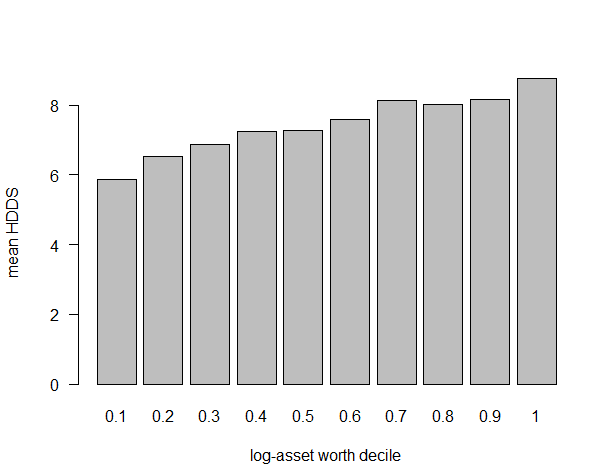
\includegraphics[width=3in]{subchapters/figures/hdds_by_lnA0}
\par\end{centering}
\caption{\label{fig:Diversity-Scores}Diversity Score changes by log asset
deciles}
\end{figure}

\begin{figure}[H]
\begin{centering}
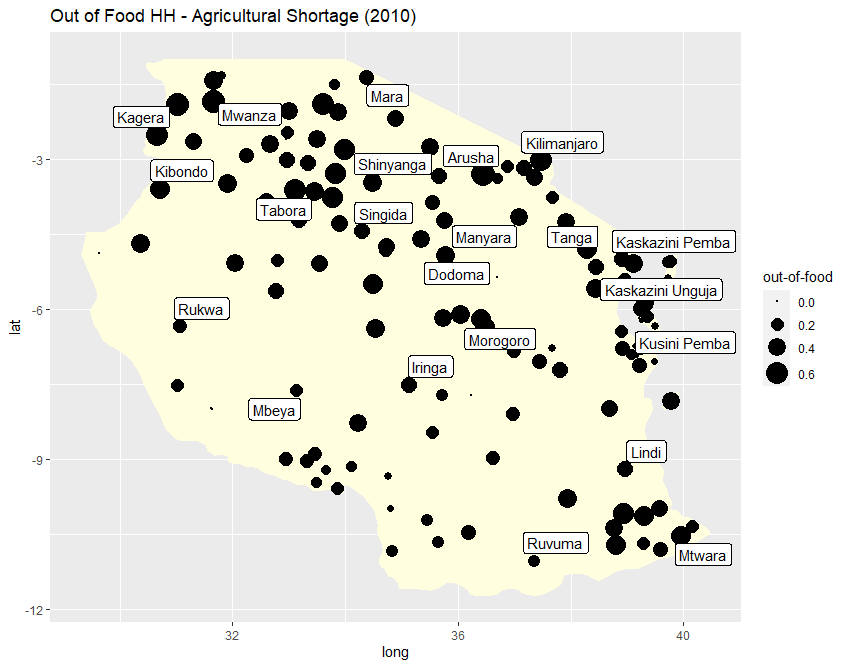
\includegraphics[width=4in]{subchapters/figures/tnz_out_food_due_to_agri_households2010}
\par\end{centering}
\caption{\label{fig:FractionAgInp}Fraction of households having run of food
due to agricultural inputs in the past year (2010)}
\end{figure}

\begin{figure}[H]
\begin{centering}
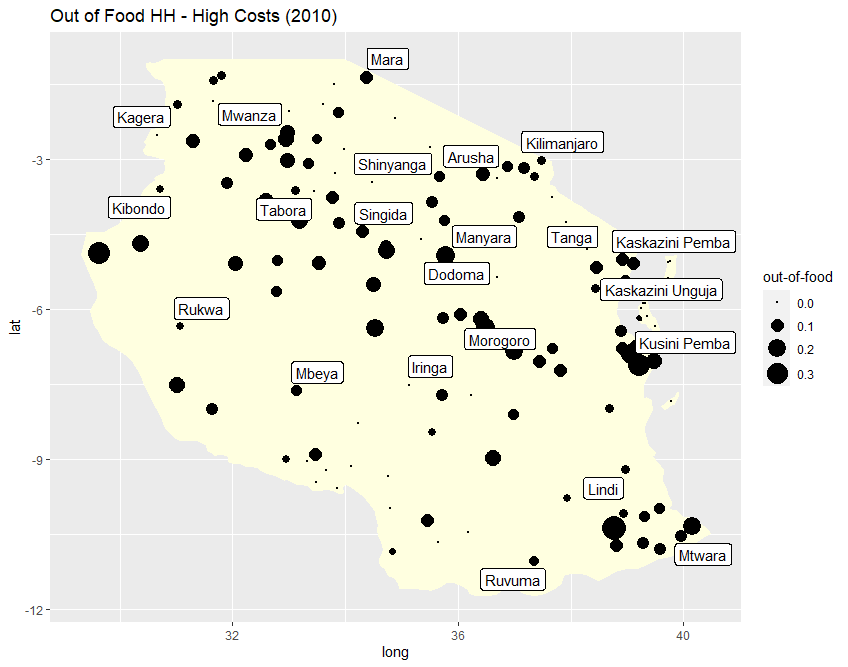
\includegraphics[width=4in]{subchapters/figures/tnz_out_food_due_to_costs_households2010}
\par\end{centering}
\caption{\label{fig:FractionHiCost}Fraction of households having run of food
due to costs in the past year (2010)}
\end{figure}

The spatial distribution of food insecurity provides us an overview
of regional disparities in the country. To survey food insecurity,
we use the directly observed food deprivation in the survey to compare
the fraction of households having run out of food (either due to lack
of agricultural inputs or high prices) in the past year across urban
and rural areas (see Figures \ref{fig:FractionAgInp} and \ref{fig:FractionHiCost}).
While the figures do suggest a significant proportion of households
running out of food in urban areas (due to high costs), the overall
hunger instances remain proportionately lower in the urban areas (when
compared to the households having run out of food due to agricultural
reasons- see Figure \ref{fig:FractionHiCost}). While the food insecurity
does not seem significantly stronger in either urban or rural areas,
the extremity of urban-rural or regional differences seems evident
from a comparison of assets and occupations. As a non-parametric view
of occupations\footnote{The variable \texttt{occupation\_rank} shown in the figure is defined
as an ordered variable indicating an income-based rank inferred from
the occupation of the head-household using the available income data
(see Table\textbf{ }Appendix III for mapping of occupations to occupation-ranks).} and value of assets-owned show (Figure \ref{fig:occupations_r_tn}),
the higher-paid occupations seems severely to urban - particularly
eastern coastal - areas in Tanzania.

\begin{figure}[h]
\begin{centering}
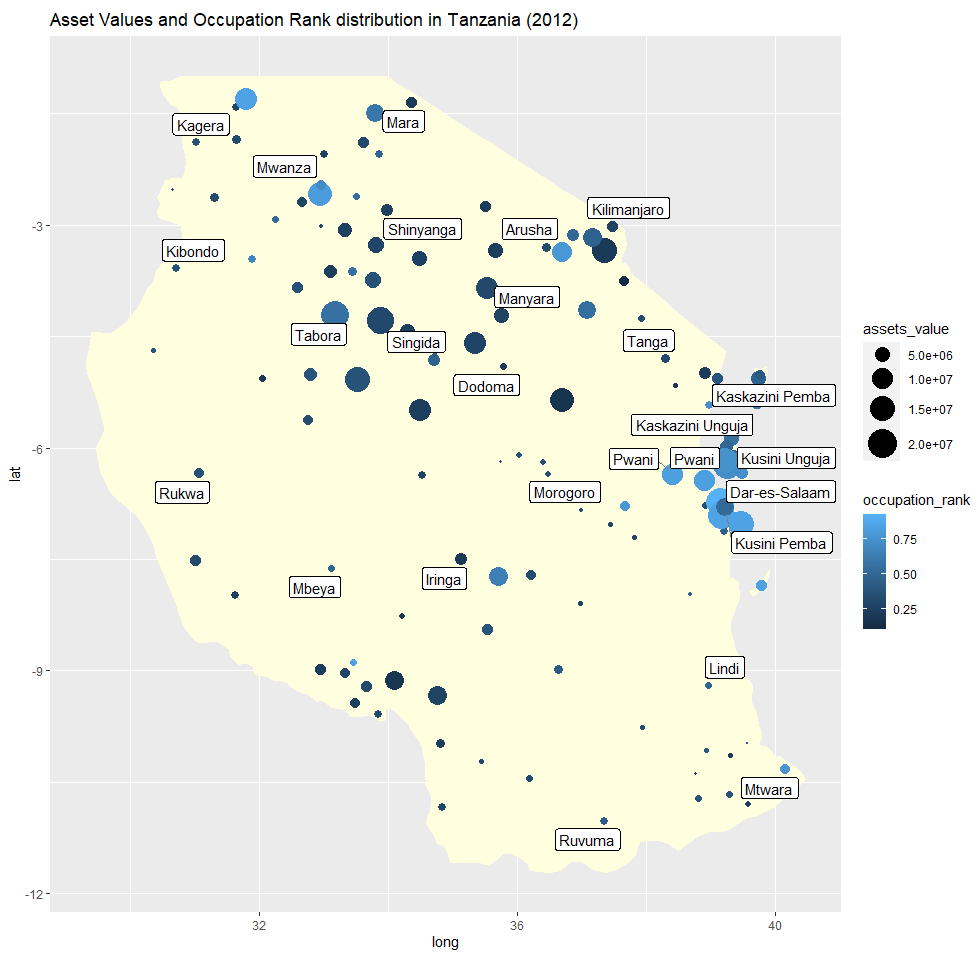
\includegraphics[width=4.5in]{subchapters/tnz_assets_occuprank_distribution_2012}
\par\end{centering}
\caption{\label{fig:occupations_r_tn}Occupations and consumer-owned assets
in Tanzania}
\end{figure}


\subsection{Results}

\noindent

The key goal of our empirical analysis is to test whether \hlw{the
effects of permanent income (as well as asset-ownership) result in
higher quality overall or if the effects are limited to specific food-categories
in Tanzania}. The disaggregated view of quality into commodities
based on FAO categories allows us to relate the choice for quality
in high-level commodity groups with the \hlw{effects of permanent
income - while also controlling with local prices in an AIDS framework.
The effect of permanent income measures seems significant on food
quality with respect to the meats-proteins commodity }. We also find
that access to higher food quality is higher in localities with access
to electricity.
\begin{center}
\begin{table}[H]
\begin{centering}
\begin{tabular}{>{\raggedright}p{2in}|>{\raggedright}p{3.5in}}
\hline 
Variable & Description\tabularnewline
\hline 
\texttt{ln\_tot\_exp} & logarithm of per-head total expenditure $x_{t}$ per household \tabularnewline
\hline 
\texttt{\small{}lp-} & base-prices for various commodities\tabularnewline
\hline 
\texttt{hsize} & number of members in a household\tabularnewline
\hline 
\texttt{age} & age of the household-head\tabularnewline
\hline 
\texttt{logA} & logarithm of sum of reported market-price of assets owned by the household\tabularnewline
\hline 
\texttt{isurban} & indicator variable specifying if the region is Dar-es-Salaam, Mbeya,
Mwanza or Magharibi Unguja(Zanzibar)\tabularnewline
\hline 
\texttt{has\_electric} & indicator variable specifying if the household uses electricity or
not\tabularnewline
\end{tabular}
\par\end{centering}
\caption{\label{tab:Control-Variables}Control Variables}
\end{table}
\par\end{center}

%[Systematic introduction of control variables]

The estimation results from the AIDS formulation - which we have specified
in Equations \ref{eq:AIDS_quality_w} and \ref{eq:AIDS_quality_lnV}
- are presented in Tables \ref{results_has_electric_2014} and \ref{results_elecassets_2014}.
The logarithm of the total expenditure \texttt{\footnotesize{}ln\_tot\_exp}
is used as the main explanatory variable in the results presented
in Table \ref{results_has_electric_2014} . In an alternative formulation
for which the results presented in Table \ref{results_elecassets_2014},
the logarithm of total household owned (long-term) assets \texttt{logA}
is used as the main explanatory variable. An important set of controls
are the prices corresponding to the food commodities - which are listed
in Table \ref{tab:GroupsModified}. As described in Section \ref{subsec:Econometric-Method},
the AIDS formulation in Equations \ref{eq:AIDS_quality_w} and \ref{eq:AIDS_quality_lnV}
use the logarithm of base-prices of food categories (commodities)
as price-controls. These are represented as the variables starting
with the prefix \texttt{\footnotesize{}lp}- (e.g. \texttt{lpdensefoods,
lpnonfresh, lpprotein }etc.) in the results presented in Tables \ref{results_has_electric_2014}
and \ref{results_elecassets_2014}. Recall that the base-price $P_{G}$
for every commodity $G$ in the Equation \ref{eq:base_price_structure}
is simply the minimum price of the goods within the commodity group
that is derived from the locally observed market prices (at the district
level) rather than the unit-values (estimated by averaging expenditure
over a locality) for goods within a commodity. Every composite commodity
in the AIDS regression (see Equations \ref{eq:AIDS_quality_w} and
\ref{eq:AIDS_quality_lnV}) thus corresponds to an \texttt{\footnotesize{}lp-}
variable. It is worth remarking that the prices of other items in
the commodity are incorporated in the price-structure that is considered
in the measurement of quality. Other important controls used for results
in Tables \ref{results_has_electric_2014} and \ref{results_elecassets_2014}
are listed in Table \ref{tab:Control-Variables}. 

Of the controls in Table \ref{tab:Control-Variables}, the indicator
variable \texttt{has\_electric }- specifies whether the household
uses electricity (used in both Tables \ref{results_has_electric_2014}
and \ref{results_elecassets_2014}) and is inferred from the field
for source of energy for lighting in the survey. Two further household
characteristics which we explore the effects of are \texttt{hsize}
(number of household members ) and \texttt{age} (age of the household-head).
Whether the households reside in urban areas or not are considered
with a indicator variable \texttt{isurban} ( indicator variable for
densely populated urban areas).
\begin{center}
\begin{table}[H]
\begin{centering}
\begin{tabular}{>{\raggedright}p{2in}|>{\raggedright}p{3.5in}}
\hline 
Variable & Description\tabularnewline
\hline 
\texttt{qcereals} & budget share for the entire commodity: cereals\tabularnewline
\hline 
\texttt{qVcereals} & quality metric for the entire commodity: cereals\tabularnewline
\hline 
\texttt{qcomplements} & budget share for the entire commodity: complements\tabularnewline
\hline 
\texttt{qVcomplements} & quality metric for the entire commodity: complements\tabularnewline
\hline 
\texttt{qfat} & budget share for the entire commodity: fat\tabularnewline
\hline 
\texttt{qVfat} & quality metric for the entire commodity: fat\tabularnewline
\hline 
\texttt{qfish} & budget share for the entire commodity: fish\tabularnewline
\hline 
\texttt{qVfish} & quality metric for the entire commodity: fish\tabularnewline
\hline 
\texttt{qfruits} & budget share for the entire commodity: fruits\tabularnewline
\hline 
\texttt{qVfruits} & quality metric for the entire commodity: fruits\tabularnewline
\hline 
\texttt{qmeatsproteins} & budget share for the entire commodity: meats-proteins\tabularnewline
\hline 
\texttt{qVmeatsproteins} & quality metric for the entire commodity: meats-proteins\tabularnewline
\hline 
\texttt{qmilk} & budget share for the entire commodity: milk\tabularnewline
\hline 
\texttt{qVmilk} & quality metric for the entire commodity: milk\tabularnewline
\hline 
\texttt{qstarches} & budget share for the entire commodity: starches\tabularnewline
\hline 
\texttt{qVstarches} & quality metric for the entire commodity: starches\tabularnewline
\hline 
\texttt{qtubers} & budget share for the entire commodity: tubers\tabularnewline
\hline 
\texttt{qVtubers} & quality metric for the entire commodity: tubers\tabularnewline
\hline 
\texttt{qveg} & budget share for the entire commodity: vegetables\tabularnewline
\hline 
\texttt{qVveg} & quality metric for the entire commodity: vegetables\tabularnewline
\end{tabular}
\par\end{centering}
\caption{\label{tab:Dependent-Variables}Dependent Variables}
\end{table}
\par\end{center}

The dependent variables of the AIDS regressions in the columns of
Tables \ref{results_has_electric_2014} and \ref{results_elecassets_2014}-
starting either with \texttt{\footnotesize{}q}- or with \texttt{\footnotesize{}qV}
- indicate the budget-share and quality metric respectively. The columns
starting with \texttt{\footnotesize{}q-} indicate the budget shares
that are used as the dependent variables in AIDS regressions (see
Equation \ref{eq:AIDS_quality_w} ) while the columns starting with
\texttt{\footnotesize{}qV- }indicate the logarithm of the quality
metric as the dependent variable (i.e. $ln\ V$ in the Equation \ref{eq:AIDS_quality_lnV}).
The list of all dependent variables are presented in Table \ref{tab:Dependent-Variables}.
Recall that the classification of items - which is based on prices-correlation
- results in the commodities and constituents good listed in Table
\ref{tab:GroupsModified}. The total number of equations (the Equations
\ref{eq:AIDS_quality_w} and \ref{eq:AIDS_quality_lnV} specified
in Section \ref{subsec:Econometric-Method}) for the estimation is
therefore $10\times2=20$ (see Appendix IV for the entire list of
estimation equations). The estimation uses a three-stage least-squares
method for systems of equations (see \cite{Zellner3SLS1992}) for
the Equations \ref{eq:AIDS_quality_w} and \ref{eq:AIDS_quality_lnV}
and with symmetry constraints specified in Section \ref{subsec:Econometric-Method}.

\subsection*{Discussion}

\noindent

%[Significance of has_electric, assets and ln_tot_exp]

The results obtained from the AIDS regression shown in Tables \ref{results_has_electric_2014}
and \ref{results_elecassets_2014} suggest a relevance of permanent
income (measured with total expenditure) and ownership of assets -
along with access to electricity - on the demand for quality in food.
While there is a some heteroskedasticity in the results (tested for
with Breush-Pagan statistic), the effects of household expenditure
and total assets owned appear significant for quality.

%[Effect of ln_tot_exp]

In Table \ref{results_has_electric_2014}, the effect of permanent
income (\texttt{ln\_tot\_exp} ) is positive on quality across all
food commodities i.e. the income-elasticities are positive for quality
within food categories (commodities). This does not seem surprising
since the income-elasticities for quality are expected to be positive
so long as a higher total expenditure \texttt{ln\_tot\_exp} is spent
on the more expensive variants (goods) within a food category (commodity).
The negative income elasticities for budget-share of some food commodities
are also predictable - if we consider that certain goods are preferred
for higher (price-based) quality and therefore lower quantity (budget
share). Of particular attention is how the budget shares show a decline
with total expenditure logarithm for commodities \texttt{fat }and
\texttt{meatsproteins} (see coefficients of \texttt{ln\_tot\_exp}
under \texttt{qfat} and \texttt{qmeatsproteins} in Table \ref{results_has_electric_2014})
. More specifically, the increase in food expenditure is associated
with less quantity (at the cost of higher quality) of \texttt{fats
}and \texttt{meatsproteins} - while quality consumed for both fats
and meats-proteins rises with higher total expenditure logarithm (see
coefficients of \texttt{ln\_tot\_exp} under \texttt{qVfat} and \texttt{qVmeatsproteins}
in Table \ref{results_has_electric_2014}). With cereals, on the other
hand, we see that the budget shares rise with higher total expenditure
logarithm (see coefficient of \texttt{ln\_tot\_exp} under \texttt{qcereals}
in Table \ref{results_has_electric_2014}) while the cereals-quality
also increases with higher total expenditure logarithm (see coefficient
of \texttt{ln\_tot\_exp} under \texttt{qVcereals} in Table \ref{results_has_electric_2014}).
The demand for quality (price-based) for meat is unlike that for cereals
in the sense that higher-income households increase both price-based
quality and quantity (budget-shares) for cereals whereas they seem
increase quality without increasing quantity (budget shares) for meats.

%[has_electric in ln_tot_exp table and the endogeneity]

Looking at the effect of access to electricity ( \texttt{has\_electric}
) in Table \ref{results_has_electric_2014}, we see a higher quality
across food categories - an effect similar to that of total expenditure
logarithm \texttt{ln\_tot\_exp }(except for fats where quality is
not significantly higher for consumers with access to electricity).
It could be argued that having access to electricity is endogenous
with higher prosperity. Thus it may simply be that those with higher
income are the one with access to electricity and have a better access
to quality through ownership of electric appliances. However, the
correlation of having access to electricity with prosperity is more
likely through being in the urban area rather through income. This
is because the indicator variable \texttt{has\_electric }used for
access to electricity is based only on the usage of electricity as
the primary source of lighting at home. The basic usage of electricity
hardly reflects the income of the household - and is more strongly
correlated with being in an area (more often urban) where electricity
is available (particularly given the sparse distribution of electricity
in Tanzania). Since availability of refrigeration facilities in a
market may improve the availability of fruits and meats in a wider
area, the positive externality through being in richer areas - one
that includes access to electricity - is more likely to be the cause
for higher quality in food categories.

%[ln_tot_exp table - hsize ]

The effects of \texttt{hsize} on quality are also worth noting - as
larger families (higher \texttt{hsize} ) corresponds to lower quality
(particularly in protein and fruits-veg) but lower their budget-share
for consumption. This suggests a pressure to maintain high quality
in larger families with children.

%[ln_tot_exp table - prices]

% g <- merge((subset(o2014,household_status==1))[,c("hhid","isurbanp","lightingfuel")],g2014,by=c("hhid"))
% g$has_electric  <- with(g,as.integer(is.element(lightingfuel,c(1,8))))
% ddply(subset(g,category=="meatsproteins"),.(isurbanp),summarise,n=median(tot_categ_exp/lp_min_price))
% fdf <- get_fao_quality_agg_df()
% fdf$logA <- log(fdf$all_assets_mtm+1e-7)
% gf <- (subset(merge(fdf[,c("hhid","logA")],g,by=c("hhid"))))
% k <- subset(gf,isurbanp==T & category=="meatsproteins") ; plot(k$logA, with(k,tot_categ_exp/lp_min_price),xlim=c(2,3.2)) 
% the asset dependence does not change - this is not apparent from the descriptive statistics

A key advantage of using the proposed framework of quality is that
it allows us to examine the effect of prices of commodities on quality.
Looking at the effect of (base-)prices (variables \texttt{lp-}) in
both Tables \ref{results_has_electric_2014} and \ref{results_elecassets_2014},
we see with \texttt{lpmeatsproteins} - for example - that the high
base-price of meats-proteins (the cheapest meat-protein available
in the district) corresponds to higher quality in \texttt{fruits}
and \texttt{veg}. Thus, the households in districts where base-price
of \texttt{meatsproteins }(price of cheapest meat-protein) is high
also avail higher quality of fruits and veg - an indication of how
meat consumption may be associated with higher income in Tanzania. 

The results in Table \ref{results_has_electric_2014} also suggest
certain substitutions in quality across some food commodities. For
example, with a rise in prices of cereals (\texttt{lpcereals}), the
quality in meats-proteins (see coefficient of \texttt{lpcereals} under
\texttt{qVmeatsproteins} in Table \ref{results_has_electric_2014})
increases but the quality in starches (see coefficient of \texttt{lpcereals}
under \texttt{qVstarches} in Table \ref{results_has_electric_2014})
and vegetables (see coefficient of \texttt{lpcereals} under \texttt{qVveg
}in Table \ref{results_has_electric_2014} ) declines - indicating
that the consumers tend to increase quality in meat-consumption while
reducing the quality for starches and veg. In other words, with higher
prices of (cheapest) meat, the consumer is more likely to increase
quality elsewhere (e.g. in fruits and vegetables) - indicating once
again how meat consumption rises with higher income.

On similar lines, we see that the quality in starches seems to drop
with rise in prices of fruits (see coefficient of \texttt{lpfruits}
under \texttt{qVstarches} in Table \ref{results_has_electric_2014})
whereas the quality in fruits does not rise with the base-price of
starches (see coefficient of \texttt{lpstarches} under \texttt{qVfruits}
in Table \ref{results_has_electric_2014}). In other words, when (cheapest)
fruit is more expensive, starch quality is also lower for consumers
whereas (cheapest) starch being more expensive does not raise the
quality of fruits for consumers. It is more often thus that the consumers
spend higher on quality in starches when the fruits become expensive
(rather than spending higher on quality in fruits when starch becomes
more expensive). A similar relation is not seen between tubers and
starches whose consumption of quality seem to move together.

The observation from the budget shares that the expenditure on \texttt{veg}
and \texttt{meatsproteins} is higher - particularly for \texttt{meatsproteins}
- in urban areas can also be verified with a simple calculation of
total expenditure divided by the commodity base-price. Estimating
the effective quantity of \texttt{meatsproteins} consumed as the \texttt{meatsproteins}
expenditure divided by its base-price, the urban areas seem to consume
about 1.61 times more \texttt{meatsproteins} and spend 1.63 times
more (comparing just expenditure) - not as much for the expenditure
on \texttt{chicken} or \texttt{fish}. With effective quantity of \texttt{veg},
the urban areas consume about 1.1 times more \texttt{meatsproteins}
and spend also about 1.1 times more than the rural areas. Looking
at the expenditures in urban and rural areas for \texttt{cereals},
we see that unlike with \texttt{meatsproteins}, the differences in
expenditure (or in effective quantity) for \texttt{cereals} across
urban and rural areas and are not wide. The expenditures also suggest
that while the consumption of \texttt{veg} rises with total expenditure
logarithm \texttt{ln\_tot\_exp} , it does not rise as much as \texttt{meatsproteins}
in urban areas and does not differ a lot from the expenditures in
rural areas.

%[assets-table]

In Table \ref{results_elecassets_2014} - where total assets logarithm
\texttt{logA} is used as the main explanatory variable instead of
total expenditure \texttt{ln\_tot\_exp} - the coefficient of total
assets logarithm is positive for meatsproteins (dependent variable:
\texttt{qmeatsproteins}) - suggesting that those with lower assets
do consume less \texttt{meatsproteins }overall. In other words, the
lower quantity of \texttt{meatsproteins }for those with low-assets-ownership
does not mean a higher quality in \texttt{meatsproteins }(compare
signs under \texttt{qmeatsproteins} of the coefficients for \texttt{logA}
and \texttt{ln\_tot\_exp} in Tables \ref{results_has_electric_2014}
and \ref{results_elecassets_2014} ). The quality consumed for meats-proteins
does rise with higher total assets logarithm as well. Comparing with
cereals, on the other hand, we see that the budget shares are lower
for those with higher total assets - even though the quality consumed
is higher.

The access to electricity ( \texttt{has\_electric} ) indicates a higher
quality across food categories in Table \ref{results_elecassets_2014}
as well. The budget shares rise for fruits and milk in Table \ref{results_elecassets_2014}
whereas they fall for fat (\texttt{qfat}) and meatsproteins (\texttt{qmeatsproteins})
- even though the quality metrics rise (both \texttt{qVfat} and \texttt{qVmeatsproteins})
for the consumers having electricity. This may be due to refrigeration
storage facilities available in certain localities. The consumption
of fish (budget shares \texttt{qfish}) is not affected by the \texttt{has\_electric
}variable as much as \texttt{meatsproteins} - suggesting a higher
local consumption for fish (likely less dependent on refrigeration
facilities overall). For fruits and milk on the other hand, both the
quality consumed and budget-share are higher for consumers with access
to electricity (see Table \ref{results_elecassets_2014}).

%[Both Tables - isurban and hsize]

In both Tables \ref{results_has_electric_2014} and \ref{results_elecassets_2014},
we see that the effect of \texttt{isurban} (apart from the base-price
$P_{G}$) on quality is significant on quality across all food categories.
This could be an indication of higher income occupations concentrated
in the eastern coast and centre of Tanzania. More specifically, quality
for meatsproteins ( \texttt{qVmeatsproteins} ) is slightly lower in
urban areas (compare coefficients of \texttt{isurban} under \texttt{qVmeatsproteins}
and \texttt{qVfruits} in both Tables \ref{results_has_electric_2014}
and \ref{results_elecassets_2014}) and is better with access to electricity.
In other words, those with no access to electricity in the urban areas
are less likely to spend higher on quality of meats-proteins compared
to the consumers in rural areas. The effects of both total expenditure
and assets-ownership are significant in the quality of consumption
for food. The access to electricity in urban environment creates clear
differences in lifestyle choices as well as dependence on higher budgets
- an effect that remains significant for access to quality in nutrition.
In summary, even though there may be some positive externality with
being in the urban areas, the differences in quality of consumption
associated with \hlw{high permanent income as well as } assets possession
remain significant. 

\hlw{While the question of whether higher quality for food can be
considered aspirational or not could be answered only after surveys
of subjective well-being of consumers, there are two observations
pertaining to determinants of aspirational consumption that we can
make from the above results. First, the demand for quality is strong
for specific food items (rather than across wider nutritional categories).
Second, the role of regional identity is likely to be strong towards
aspirational consumption due to the extreme life-style differences
between urban and rural areas. The observations seem to be supported
by the presence of a strong positive externality with rich surroundings
in the data on subjective-welfare in LSMS survey in Tanzania as well}(\cite{AstebiCarbonell2019}).

%The consumption such as food, where a higher quality may be always in the market, it is always difficult and therefore the processes of snob becoming a bandwagon is less of a concern.

%[Robustness]

\subsection*{Robustness Checks}

\noindent

As a test of the robustness of results, we calculate the food-quality
using the market-provided prices and instead of the expenditure reported
by the household. More specifically, in the results shown in Tables
\ref{results_has_electric_2014} and \ref{results_elecassets_2014},
we have used diary-costs on goods as reported by the household - costs
that are recorded by the LSMS for the goods that were consumed from
purchases in the last week. If a household didn't purchase anything
in the past week, there would only be quantities consumed (not costs)
that would be reported for the household in the diary. Since we have
the market-prices available, another way to calculate costs, budget-shares
and quality would be to infer costs as the multiple of market-prices
from the quantities consumed in the past week (which is reported for
all households regardless of whether they had purchased something
in the last week or not). Recalculating quality and budget shares
still shows us the same economic and statistical significance (results
available on request) of electricity and household assets in quality
of food categories (commodities).

% The education rank is set to 1 for all pre-primary levels, to rank 2 for until the completion of primary education, to rank 3 for up to the secondary education level and to 4 for all higher education levels (higher-secondary, university etc.). For instance, the primary school leaving exam is taken at D7 in Tanzania and corresponds to the education rank 2 ; all standards above D7 correspond to the education rank 3 and so forth. The complete mapping is provided in Table \ref{education_rank_tnz}. The argument for using the education-ranks as instruments is simply that a higher food quality in food is unlikely to be favoured by differences in education levels. In other words, while quality - in general - could be constrained due to occupational structures in the economy, there are few reasons to think that purchases of food could be influenced by one's education level except through the permanent income measure.

% Add - \rowcolor{Gray} after \\ 

\begin{landscape}
\begin{table}
\caption{\label{results_has_electric_2014}reg3 results with electricity usage indicator control (2014)} 
\resizebox{\columnwidth}{!}{

\def\sym#1{\ifmmode^{#1}\else\(^{#1}\)\fi} \begin{tabular}{l*{21}{c}} \hline\hline  & \multicolumn{1}{c}{} & \multicolumn{1}{c}{(1)} & \multicolumn{1}{c}{(2)} & \multicolumn{1}{c}{(3)} & \multicolumn{1}{c}{(4)} & \multicolumn{1}{c}{(5)} & \multicolumn{1}{c}{(6)} & \multicolumn{1}{c}{(7)} & \multicolumn{1}{c}{(8)} & \multicolumn{1}{c}{(9)} & \multicolumn{1}{c}{(10)} & \multicolumn{1}{c}{(11)} & \multicolumn{1}{c}{(12)} & \multicolumn{1}{c}{(13)} & \multicolumn{1}{c}{(14)} & \multicolumn{1}{c}{(15)} & \multicolumn{1}{c}{(16)} & \multicolumn{1}{c}{(17)} & \multicolumn{1}{c}{(18)} & \multicolumn{1}{c}{(19)} & \multicolumn{1}{c}{(20)} \\ & \multicolumn{1}{c}{} & \multicolumn{1}{c}{qcereals} & \multicolumn{1}{c}{qcomplements} & \multicolumn{1}{c}{qfat} & \multicolumn{1}{c}{qfish} & \multicolumn{1}{c}{qfruits} & \multicolumn{1}{c}{qmeatsproteins} & \multicolumn{1}{c}{qmilk} & \multicolumn{1}{c}{qstarches} & \multicolumn{1}{c}{qtubers} & \multicolumn{1}{c}{qVcereals} & \multicolumn{1}{c}{qVcomplements} & \multicolumn{1}{c}{qveg} & \multicolumn{1}{c}{qVfat} & \multicolumn{1}{c}{qVfish} & \multicolumn{1}{c}{qVfruits} & \multicolumn{1}{c}{qVmeatsproteins} & \multicolumn{1}{c}{qVmilk} & \multicolumn{1}{c}{qVstarches} & \multicolumn{1}{c}{qVtubers} & \multicolumn{1}{c}{qVveg}\\ \hline
\\ \rowcolor{Gray}  & isurban & -0.0317$^{***}$ & -0.0170$^{***}$ & 0.0002 & 0.0197$^{***}$ & 0.0094$^{*}$ & 0.0118 & -0.0041$^{*}$ & 0.0074$^{**}$ & -0.0039 & -0.1542$^{**}$ & 0.0360 & 0.0055$^{*}$ & -0.8281 & 0.0484$^{*}$ & 0.1402$^{**}$ & -0.4567$^{***}$ & -0.0581$^{***}$ & 0.0190 & 0.0577 & 0.1297$^{***}$\\ \rowcolor{Gray} &  & (0.000) & (0.000) & (0.964) & (0.000) & (0.020) & (0.120) & (0.043) & (0.007) & (0.260) & (0.004) & (0.104) & (0.021) & (0.283) & (0.011) & (0.003) & (0.000) & (0.000) & (0.764) & (0.121) & (0.000)
\\ & has\_electric & -0.0641$^{***}$ & -0.0095$^{*}$ & 0.0019 & -0.0050 & 0.0253$^{***}$ & 0.0296$^{***}$ & 0.0066$^{**}$ & 0.0175$^{***}$ & -0.0041 & 0.0828 & 0.0294 & -0.0008 & -1.4587 & 0.0367 & 0.2107$^{***}$ & 0.4544$^{***}$ & 0.0939$^{***}$ & 0.5391$^{***}$ & 0.1254$^{**}$ & 0.1341$^{***}$\\ &  & (0.000) & (0.029) & (0.653) & (0.398) & (0.000) & (0.000) & (0.002) & (0.000) & (0.278) & (0.136) & (0.206) & (0.767) & (0.071) & (0.069) & (0.000) & (0.000) & (0.000) & (0.000) & (0.001) & (0.000)
\\ \rowcolor{Gray} & hh\_age & 0.0002 & 0.0002 & -0.0003$^{**}$ & 0.0004$^{*}$ & -0.0002$^{*}$ & 0.0002 & -0.0000 & -0.0001 & -0.0002$^{*}$ & 0.0023 & 0.0008 & 0.0000 & -0.0081 & -0.0005 & -0.0027$^{*}$ & 0.0044$^{**}$ & -0.0003 & -0.0019 & -0.0024$^{*}$ & -0.0013$^{**}$\\ \rowcolor{Gray} &  & (0.407) & (0.057) & (0.009) & (0.015) & (0.020) & (0.274) & (0.560) & (0.301) & (0.044) & (0.100) & (0.180) & (0.883) & (0.688) & (0.321) & (0.028) & (0.003) & (0.403) & (0.253) & (0.015) & (0.004)\\ & hsize & -0.0035$^{**}$ & 0.0042$^{***}$ & 0.0026$^{***}$ & 0.0038$^{***}$ & -0.0018$^{**}$ & -0.0003 & -0.0014$^{***}$ & -0.0009$^{*}$ & -0.0004 & -0.0887$^{***}$ & -0.0310$^{***}$ & -0.0009$^{*}$ & 0.2308$^{*}$ & 0.0000 & -0.0484$^{***}$ & -0.0574$^{***}$ & -0.0141$^{***}$ & -0.0294$^{**}$ & -0.0228$^{***}$ & -0.0208$^{***}$\\ &  & (0.004) & (0.000) & (0.000) & (0.000) & (0.003) & (0.808) & (0.000) & (0.029) & (0.478) & (0.000) & (0.000) & (0.011) & (0.049) & (0.994) & (0.000) & (0.000) & (0.000) & (0.002) & (0.000) & (0.000)\\ \rowcolor{Gray} & ln\_tot\_exp & 0.0641$^{***}$ & -0.0091$^{***}$ & -0.0326$^{***}$ & -0.0052$^{*}$ & 0.0095$^{***}$ & -0.0532$^{***}$ & 0.0042$^{***}$ & 0.0112$^{***}$ & 0.0049$^{**}$ & 0.6292$^{***}$ & 0.2089$^{***}$ & -0.0002 & 0.6893$^{*}$ & 0.1220$^{***}$ & 0.3857$^{***}$ & 0.5941$^{***}$ & 0.0799$^{***}$ & 0.4104$^{***}$ & 0.1870$^{***}$ & 0.1455$^{***}$\\ \rowcolor{Gray} &  & (0.000) & (0.000) & (0.000) & (0.025) & (0.000) & (0.000) & (0.000) & (0.000) & (0.001) & (0.000) & (0.000) & (0.855) & (0.032) & (0.000) & (0.000) & (0.000) & (0.000) & (0.000) & (0.000) & (0.000)\\ & lpcereals & -0.0060 & 0.0001 & -0.0014 & 0.0031 & 0.0166$^{***}$ & -0.0166$^{***}$ & -0.0011 & 0.0023 & 0.0049$^{**}$ & -1.5037$^{***}$ & 0.0516$^{**}$ & -0.0018 & 0.6404 & 0.0194 & 0.0237 & 0.3641$^{***}$ & -0.0228$^{*}$ & -0.1978$^{***}$ & -0.0431 & -0.0503$^{***}$\\ &  & (0.253) & (0.970) & (0.397) & (0.187) & (0.000) & (0.000) & (0.252) & (0.133) & (0.002) & (0.000) & (0.001) & (0.217) & (0.247) & (0.100) & (0.477) & (0.000) & (0.012) & (0.000) & (0.088) & (0.000)\\ \rowcolor{Gray} & lpcomplements & 0.0001 & 0.0019 & 0.0003 & -0.0012 & 0.0016 & 0.0060 & -0.0005 & 0.0015 & -0.0066$^{***}$ & 1.5261$^{***}$ & -0.0461 & -0.0031 & 4.4315$^{**}$ & -0.0882$^{**}$ & 0.0245 & 1.7650$^{***}$ & 0.0163 & 0.4861$^{***}$ & 0.0484 & -0.1422$^{***}$\\\rowcolor{Gray}  &  & (0.970) & (0.805) & (0.768) & (0.429) & (0.615) & (0.273) & (0.522) & (0.263) & (0.000) & (0.000) & (0.260) & (0.058) & (0.002) & (0.001) & (0.767) & (0.000) & (0.419) & (0.000) & (0.440) & (0.000)\\ & lpfat & -0.0014 & 0.0003 & 0.0002 & 0.0013 & -0.0020$^{*}$ & 0.0032 & -0.0008 & -0.0019$^{**}$ & 0.0013 & -0.0110 & -0.0236$^{***}$ & -0.0002 & -8.8267$^{***}$ & 0.0064 & 0.0098 & -0.0016 & -0.0028 & -0.1016$^{***}$ & 0.0115 & -0.0025\\ &  & (0.397) & (0.768) & (0.850) & (0.202) & (0.044) & (0.075) & (0.077) & (0.003) & (0.065) & (0.419) & (0.000) & (0.714) & (0.000) & (0.156) & (0.426) & (0.916) & (0.423) & (0.000) & (0.224) & (0.590)\\ \rowcolor{Gray} & lpfish & 0.0031 & -0.0012 & 0.0013 & 0.0052$^{*}$ & -0.0027 & -0.0041 & -0.0023$^{***}$ & -0.0015 & 0.0030$^{**}$ & 0.0100 & -0.0214$^{*}$ & -0.0007 & -0.4615 & 0.0413$^{***}$ & 0.0326 & -0.0128 & -0.0078 & 0.0209 & 0.0306$^{*}$ & 0.0004\\ \rowcolor{Gray} &  & (0.187) & (0.429) & (0.202) & (0.013) & (0.059) & (0.110) & (0.000) & (0.104) & (0.003) & (0.606) & (0.011) & (0.382) & (0.111) & (0.000) & (0.063) & (0.542) & (0.116) & (0.374) & (0.023) & (0.946)\\ & lpfruits & 0.0166$^{***}$ & 0.0016 & -0.0020$^{*}$ & -0.0027 & 0.0079$^{*}$ & -0.0243$^{***}$ & 0.0015$^{*}$ & 0.0023$^{*}$ & 0.0005 & 0.0458 & -0.0046 & -0.0013 & -0.9906 & -0.0084 & -0.3593$^{***}$ & -0.0227 & -0.0027 & -0.1496$^{**}$ & -0.0263 & -0.0169\\ &  & (0.000) & (0.615) & (0.044) & (0.059) & (0.010) & (0.000) & (0.028) & (0.043) & (0.632) & (0.259) & (0.795) & (0.301) & (0.112) & (0.498) & (0.000) & (0.601) & (0.773) & (0.002) & (0.343) & (0.195)\\ \rowcolor{Gray} & lpmeatsproteins & -0.0166$^{***}$ & 0.0060 & 0.0032 & -0.0041 & -0.0243$^{***}$ & 0.0382$^{***}$ & 0.0017 & -0.0054$^{**}$ & -0.0044$^{*}$ & -0.0368 & 0.0432 & 0.0058$^{**}$ & 8.0136$^{***}$ & 0.0343 & 0.1864$^{**}$ & -2.2568$^{***}$ & 0.0109 & -0.0440 & -0.0364 & 0.1751$^{***}$\\ \rowcolor{Gray} &  & (0.000) & (0.273) & (0.075) & (0.110) & (0.000) & (0.000) & (0.153) & (0.003) & (0.012) & (0.593) & (0.153) & (0.002) & (0.000) & (0.104) & (0.003) & (0.000) & (0.486) & (0.597) & (0.438) & (0.000)\\ & lpmilk & -0.0011 & -0.0005 & -0.0008 & -0.0023$^{***}$ & 0.0015$^{*}$ & 0.0017 & 0.0019$^{***}$ & 0.0001 & -0.0014$^{**}$ & 0.0094 & -0.0048 & 0.0009$^{*}$ & -0.2357 & -0.0076$^{*}$ & 0.0283$^{**}$ & -0.0062 & 0.0176$^{***}$ & 0.0107 & 0.0017 & 0.0032\\ &  & (0.252) & (0.522) & (0.077) & (0.000) & (0.028) & (0.153) & (0.000) & (0.752) & (0.001) & (0.333) & (0.257) & (0.023) & (0.109) & (0.016) & (0.001) & (0.554) & (0.000) & (0.369) & (0.806) & (0.330)\\\rowcolor{Gray}  & lpstarches & 0.0023 & 0.0015 & -0.0019$^{**}$ & -0.0015 & 0.0023$^{*}$ & -0.0054$^{**}$ & 0.0001 & 0.0032$^{**}$ & -0.0002 & 0.0228 & 0.0239$^{**}$ & -0.0003 & -0.2865 & 0.0002 & 0.0124 & 0.0015 & -0.0043 & -0.0307 & -0.0022 & -0.0020\\ \rowcolor{Gray} &  & (0.133) & (0.263) & (0.003) & (0.104) & (0.043) & (0.003) & (0.752) & (0.001) & (0.699) & (0.173) & (0.001) & (0.598) & (0.260) & (0.962) & (0.415) & (0.936) & (0.293) & (0.145) & (0.852) & (0.715)\\ & lptubers & 0.0049$^{**}$ & -0.0066$^{***}$ & 0.0013 & 0.0030$^{**}$ & 0.0005 & -0.0044$^{*}$ & -0.0014$^{**}$ & -0.0002 & 0.0037$^{***}$ & -0.0097 & 0.0020 & -0.0007 & -0.6671$^{**}$ & 0.0180$^{***}$ & -0.0171 & 0.0468$^{**}$ & -0.0108$^{**}$ & -0.0172 & 0.0179 & 0.0015\\ &  & (0.002) & (0.000) & (0.065) & (0.003) & (0.632) & (0.012) & (0.001) & (0.699) & (0.000) & (0.479) & (0.730) & (0.234) & (0.001) & (0.000) & (0.169) & (0.002) & (0.002) & (0.303) & (0.073) & (0.753)
\\ \rowcolor{Gray} & lpveg & -0.0018$^{***}$ & -0.0031$^{***}$ & -0.0002$^{***}$ & -0.0007$^{***}$ & -0.0013 & 0.0058$^{***}$ & 0.0009$^{*}$ & -0.0003$^{***}$ & -0.0007 & -0.0530$^{***}$ & -0.0202$^{***}$ & 0.0014$^{**}$ & -1.6173 & -0.0154$^{***}$ & 0.0586$^{***}$ & 0.1228$^{***}$ & 0.0062$^{***}$ & 0.0231$^{***}$ & -0.0021$^{***}$ & 0.0337$^{***}$
\\ \rowcolor{Gray} &  & (0.217) & (0.058) & (0.714) & (0.382) & (0.301) & (0.002) & (0.023) & (0.598) & (0.234) & (0.011) & (0.028) & (0.157) & (0.000) & (0.017) & (0.002) & (0.000) & (0.205) & (0.365) & (0.886) & (0.000)
\\ & \_cons & -0.6042$^{***}$ & 0.1824$^{***}$ & 0.5310$^{***}$ & 0.1178$^{***}$ & -0.0430 & 0.9945$^{***}$ & -0.0289$^{*}$ & -0.1060$^{***}$ & -0.0190 & -8.3633$^{***}$ & -1.7428$^{***}$ & 0.0398$^{**}$ & -2.3817 & -1.0892$^{***}$ & -4.0316$^{***}$ & -6.9911$^{***}$ & -0.8506$^{***}$ & -5.2349$^{***}$ & -2.0281$^{***}$ & -1.2673$^{***}$\\ &  & (0.000) & (0.000) & (0.000) & (0.000) & (0.068) & (0.000) & (0.012) & (0.000) & (0.347) & (0.000) & (0.000) & (0.004) & (0.623) & (0.000) & (0.000) & (0.000) & (0.000) & (0.000) & (0.000) & (0.000)

\\ \hline\hline  \multicolumn{2}{l}{\footnotesize \textit{p}-values in parentheses}\\ \multicolumn{2}{l}{\footnotesize \sym{*} \(p<0.05\), \sym{**} \(p<0.01\), \sym{***} \(p<0.001\)}\\ \end{tabular}

}
\end{table} \end{landscape} 


\begin{landscape}
\begin{table}
\caption{\label{results_elecassets_2014}reg3 results with total assets (logarithm) and electricity usage indicator control  (2014)}
\resizebox{\columnwidth}{!}{

\def\sym#1{\ifmmode^{#1}\else\(^{#1}\)\fi} \begin{tabular}{l*{21}{c}} \hline\hline  & \multicolumn{1}{c}{} & \multicolumn{1}{c}{(1)} & \multicolumn{1}{c}{(2)} & \multicolumn{1}{c}{(3)} & \multicolumn{1}{c}{(4)} & \multicolumn{1}{c}{(5)} & \multicolumn{1}{c}{(6)} & \multicolumn{1}{c}{(7)} & \multicolumn{1}{c}{(8)} & \multicolumn{1}{c}{(9)} & \multicolumn{1}{c}{(10)} & \multicolumn{1}{c}{(11)} & \multicolumn{1}{c}{(12)} & \multicolumn{1}{c}{(13)} & \multicolumn{1}{c}{(14)} & \multicolumn{1}{c}{(15)} & \multicolumn{1}{c}{(16)} & \multicolumn{1}{c}{(17)} & \multicolumn{1}{c}{(18)} & \multicolumn{1}{c}{(19)} & \multicolumn{1}{c}{(20)} \\ & \multicolumn{1}{c}{} & \multicolumn{1}{c}{qcereals} & \multicolumn{1}{c}{qcomplements} & \multicolumn{1}{c}{qfat} & \multicolumn{1}{c}{qfish} & \multicolumn{1}{c}{qfruits} & \multicolumn{1}{c}{qmeatsproteins} & \multicolumn{1}{c}{qmilk} & \multicolumn{1}{c}{qstarches} & \multicolumn{1}{c}{qtubers} & \multicolumn{1}{c}{qVcereals} & \multicolumn{1}{c}{qVcomplements} & \multicolumn{1}{c}{qveg} & \multicolumn{1}{c}{qVfat} & \multicolumn{1}{c}{qVfish} & \multicolumn{1}{c}{qVfruits} & \multicolumn{1}{c}{qVmeatsproteins} & \multicolumn{1}{c}{qVmilk} & \multicolumn{1}{c}{qVstarches} & \multicolumn{1}{c}{qVtubers} & \multicolumn{1}{c}{qVveg}\\ \hline

\\ \rowcolor{Gray} & isurban & -0.0134 & -0.0197$^{***}$ & -0.0062 & 0.0194$^{***}$ & 0.0104$^{**}$ & -0.0028 & -0.0040$^{*}$ & 0.0079$^{**}$ & -0.0024 & -0.0367 & 0.0658$^{**}$ & 0.0058$^{*}$ & -0.7816 & 0.0705$^{***}$ & 0.2010$^{***}$ & -0.3775$^{***}$ & -0.0484$^{**}$ & 0.0675 & 0.0893$^{*}$ & 0.1544$^{***}$\\ \rowcolor{Gray} &  & (0.111) & (0.000) & (0.133) & (0.000) & (0.009) & (0.724) & (0.044) & (0.004) & (0.484) & (0.526) & (0.005) & (0.015) & (0.310) & (0.000) & (0.000) & (0.000) & (0.001) & (0.295) & (0.018) & (0.000)\\ & has\_electric & -0.0047 & -0.0210$^{***}$ & -0.0211$^{***}$ & -0.0043 & 0.0298$^{***}$ & -0.0172$^{*}$ & 0.0078$^{***}$ & 0.0217$^{***}$ & 0.0018 & 0.4745$^{***}$ & 0.1259$^{***}$ & 0.0003 & -1.3344 & 0.1183$^{***}$ & 0.4277$^{***}$ & 0.7374$^{***}$ & 0.1332$^{***}$ & 0.7203$^{***}$ & 0.2375$^{***}$ & 0.2203$^{***}$\\ &  & (0.594) & (0.000) & (0.000) & (0.457) & (0.000) & (0.034) & (0.000) & (0.000) & (0.635) & (0.000) & (0.000) & (0.911) & (0.094) & (0.000) & (0.000) & (0.000) & (0.000) & (0.000) & (0.000) & (0.000)\\ \rowcolor{Gray} & logA & -0.0077$^{***}$ & 0.0042$^{***}$ & -0.0016 & -0.0043$^{***}$ & 0.0021$^{*}$ & 0.0045$^{**}$ & 0.0014$^{**}$ & 0.0031$^{***}$ & -0.0019$^{*}$ & 0.0633$^{***}$ & 0.0464$^{***}$ & -0.0010$^{*}$ & 0.2649 & 0.0042 & 0.0521$^{***}$ & 0.1156$^{***}$ & 0.0146$^{***}$ & 0.0958$^{***}$ & 0.0191$^{*}$ & 0.0156$^{***}$\\ \rowcolor{Gray} &  & (0.000) & (0.000) & (0.084) & (0.000) & (0.013) & (0.008) & (0.001) & (0.000) & (0.015) & (0.000) & (0.000) & (0.049) & (0.105) & (0.316) & (0.000) & (0.000) & (0.000) & (0.000) & (0.018) & (0.000)\\ & hh\_age & -0.0001 & 0.0002 & -0.0000 & 0.0005$^{**}$ & -0.0004$^{**}$ & 0.0005$^{*}$ & -0.0001 & -0.0002$^{**}$ & -0.0002 & -0.0036$^{*}$ & -0.0018$^{**}$ & 0.0000 & -0.0196 & -0.0015$^{**}$ & -0.0067$^{***}$ & -0.0027 & -0.0012$^{**}$ & -0.0071$^{***}$ & -0.0042$^{***}$ & -0.0027$^{***}$\\ &  & (0.775) & (0.123) & (0.910) & (0.001) & (0.001) & (0.026) & (0.077) & (0.002) & (0.062) & (0.019) & (0.003) & (0.584) & (0.339) & (0.006) & (0.000) & (0.096) & (0.002) & (0.000) & (0.000) & (0.000)\\ \rowcolor{Gray} & hsize & 0.0036$^{**}$ & 0.0024$^{***}$ & 0.0003 & 0.0045$^{***}$ & -0.0016$^{*}$ & -0.0058$^{***}$ & -0.0014$^{***}$ & -0.0008 & 0.0005 & -0.0519$^{***}$ & -0.0249$^{***}$ & -0.0007 & 0.2275 & 0.0094$^{**}$ & -0.0289$^{***}$ & -0.0355$^{***}$ & -0.0109$^{***}$ & -0.0187 & -0.0117 & -0.0124$^{***}$\\ \rowcolor{Gray} &  & (0.008) & (0.000) & (0.673) & (0.000) & (0.015) & (0.000) & (0.000) & (0.091) & (0.387) & (0.000) & (0.000) & (0.071) & (0.061) & (0.003) & (0.000) & (0.000) & (0.000) & (0.067) & (0.052) & (0.000)\\ & lpcereals & 0.0015 & -0.0017 & -0.0082$^{***}$ & 0.0024 & 0.0189$^{***}$ & -0.0221$^{***}$ & 0.0001 & 0.0056$^{***}$ & 0.0057$^{***}$ & -1.4272$^{***}$ & 0.0747$^{***}$ & -0.0021 & 0.6073 & 0.0339$^{**}$ & 0.0758$^{*}$ & 0.4352$^{***}$ & -0.0096 & -0.1343$^{**}$ & -0.0203 & -0.0341$^{**}$\\ &  & (0.788) & (0.560) & (0.000) & (0.324) & (0.000) & (0.000) & (0.913) & (0.000) & (0.000) & (0.000) & (0.000) & (0.163) & (0.272) & (0.006) & (0.028) & (0.000) & (0.299) & (0.003) & (0.430) & (0.008)\\ \rowcolor{Gray} & lpcomplements & -0.0017 & 0.0030 & 0.0017 & -0.0008 & 0.0001 & 0.0076 & -0.0009 & 0.0004 & -0.0066$^{***}$ & 1.3209$^{***}$ & -0.1476$^{**}$ & -0.0028 & 3.5007$^{*}$ & -0.1468$^{***}$ & -0.1352 & 1.4214$^{***}$ & -0.0148 & 0.3250$^{**}$ & -0.0329 & -0.2106$^{***}$\\ \rowcolor{Gray} &  & (0.560) & (0.692) & (0.124) & (0.587) & (0.962) & (0.165) & (0.262) & (0.756) & (0.000) & (0.000) & (0.001) & (0.079) & (0.013) & (0.000) & (0.112) & (0.000) & (0.472) & (0.004) & (0.603) & (0.000)\\ & lpfat & -0.0082$^{***}$ & 0.0017 & 0.0038$^{***}$ & 0.0013 & -0.0030$^{**}$ & 0.0088$^{***}$ & -0.0013$^{**}$ & -0.0033$^{***}$ & 0.0005 & -0.0690$^{***}$ & -0.0407$^{***}$ & -0.0003 & -8.8596$^{***}$ & -0.0059 & -0.0261$^{*}$ & -0.0518$^{**}$ & -0.0109$^{**}$ & -0.1391$^{***}$ & -0.0064 & -0.0160$^{**}$\\ &  & (0.000) & (0.124) & (0.000) & (0.197) & (0.002) & (0.000) & (0.002) & (0.000) & (0.484) & (0.000) & (0.000) & (0.589) & (0.000) & (0.204) & (0.040) & (0.001) & (0.002) & (0.000) & (0.500) & (0.001)\\ \rowcolor{Gray} & lpfish & 0.0024 & -0.0008 & 0.0013 & 0.0047$^{*}$ & -0.0024 & -0.0034 & -0.0023$^{***}$ & -0.0013 & 0.0027$^{**}$ & 0.0141 & -0.0179$^{*}$ & -0.0009 & -0.4367 & 0.0412$^{***}$ & 0.0364$^{*}$ & -0.0039 & -0.0072 & 0.0279 & 0.0314$^{*}$ & 0.0011\\ \rowcolor{Gray} &  & (0.324) & (0.587) & (0.197) & (0.023) & (0.086) & (0.191) & (0.000) & (0.158) & (0.006) & (0.497) & (0.042) & (0.296) & (0.132) & (0.000) & (0.045) & (0.864) & (0.157) & (0.245) & (0.022) & (0.868)\\ & lpfruits & 0.0189$^{***}$ & 0.0001 & -0.0030$^{**}$ & -0.0024 & 0.0082$^{**}$ & -0.0260$^{***}$ & 0.0017$^{*}$ & 0.0028$^{*}$ & 0.0008 & 0.0937$^{*}$ & 0.0149 & -0.0012 & -0.8222 & 0.0065 & -0.3217$^{***}$ & 0.0516 & 0.0053 & -0.1163$^{*}$ & -0.0070 & -0.0003\\ &  & (0.000) & (0.962) & (0.002) & (0.086) & (0.008) & (0.000) & (0.012) & (0.013) & (0.409) & (0.027) & (0.423) & (0.357) & (0.188) & (0.615) & (0.000) & (0.281) & (0.578) & (0.020) & (0.805) & (0.983)\\ \rowcolor{Gray} & lpmeatsproteins & -0.0221$^{***}$ & 0.0076 & 0.0088$^{***}$ & -0.0034 & -0.0260$^{***}$ & 0.0423$^{***}$ & 0.0005 & -0.0086$^{***}$ & -0.0051$^{**}$ & 0.0170 & 0.0843$^{**}$ & 0.0060$^{**}$ & 8.6268$^{***}$ & 0.0567$^{*}$ & 0.2325$^{***}$ & -2.1152$^{***}$ & 0.0163 & -0.0114 & -0.0076 & 0.2018$^{***}$\\ \rowcolor{Gray} &  & (0.000) & (0.165) & (0.000) & (0.191) & (0.000) & (0.000) & (0.689) & (0.000) & (0.004) & (0.813) & (0.008) & (0.002) & (0.000) & (0.010) & (0.000) & (0.000) & (0.310) & (0.893) & (0.872) & (0.000)\\ & lpmilk & 0.0001 & -0.0009 & -0.0013$^{**}$ & -0.0023$^{***}$ & 0.0017$^{*}$ & 0.0005 & 0.0020$^{***}$ & 0.0005 & -0.0012$^{**}$ & 0.0279$^{**}$ & 0.0021 & 0.0009$^{*}$ & -0.1894 & -0.0029 & 0.0411$^{***}$ & 0.0164 & 0.0204$^{***}$ & 0.0241$^{*}$ & 0.0082 & 0.0084$^{*}$\\ &  & (0.913) & (0.262) & (0.002) & (0.000) & (0.012) & (0.689) & (0.000) & (0.256) & (0.003) & (0.007) & (0.629) & (0.021) & (0.198) & (0.379) & (0.000) & (0.152) & (0.000) & (0.045) & (0.231) & (0.015)\\ \rowcolor{Gray}  & lpstarches & 0.0056$^{***}$ & 0.0004 & -0.0033$^{***}$ & -0.0013 & 0.0028$^{*}$ & -0.0086$^{***}$ & 0.0005 & 0.0040$^{***}$ & 0.0002 & 0.0770$^{***}$ & 0.0452$^{***}$ & -0.0002 & -0.1288 & 0.0148$^{**}$ & 0.0509$^{**}$ & 0.0721$^{***}$ & 0.0040 & 0.0087 & 0.0177 & 0.0142$^{*}$\\ \rowcolor{Gray} &  & (0.000) & (0.756) & (0.000) & (0.158) & (0.013) & (0.000) & (0.256) & (0.000) & (0.788) & (0.000) & (0.000) & (0.704) & (0.610) & (0.007) & (0.001) & (0.000) & (0.325) & (0.681) & (0.126) & (0.015)\\ & lptubers & 0.0057$^{***}$ & -0.0066$^{***}$ & 0.0005 & 0.0027$^{**}$ & 0.0008 & -0.0051$^{**}$ & -0.0012$^{**}$ & 0.0002 & 0.0037$^{***}$ & 0.0020 & 0.0065 & -0.0008 & -0.6590$^{**}$ & 0.0197$^{***}$ & -0.0094 & 0.0583$^{***}$ & -0.0090$^{*}$ & -0.0069 & 0.0209$^{*}$ & 0.0037\\ &  & (0.000) & (0.000) & (0.484) & (0.006) & (0.409) & (0.004) & (0.003) & (0.788) & (0.000) & (0.892) & (0.292) & (0.184) & (0.001) & (0.000) & (0.463) & (0.000) & (0.011) & (0.684) & (0.040) & (0.452)
\\ \rowcolor{Gray} & lpveg & -0.0021$^{***}$ & -0.0028 & -0.0003$^{***}$ & -0.0009$^{***}$ & -0.0012$^{***}$ & 0.0060$^{***}$ & 0.0009 & -0.0002 & -0.0008$^{***}$ & -0.0564$^{**}$ & -0.0215$^{***}$ & 0.0013$^{***}$ & -1.6391 & -0.0172$^{***}$ & 0.0558$^{***}$ & 0.1160 & 0.0056 & 0.0223$^{**}$ & -0.0040$^{*}$ & 0.0317$^{***}$
\\ \rowcolor{Gray}  &  & (0.163) & (0.079) & (0.589) & (0.296) & (0.357) & (0.002) & (0.021) & (0.704) & (0.184) & (0.010) & (0.026) & (0.188) & (0.000) & (0.011) & (0.005) & (0.000) & (0.264) & (0.391) & (0.784) & (0.000)
\\ & \_cons & 0.3323$^{***}$ & 0.0112 & 0.1167$^{***}$ & 0.0995$^{***}$ & 0.0596$^{***}$ & 0.2383$^{***}$ & 0.0104 & 0.0083 & 0.0677$^{***}$ & -0.5637$^{**}$ & 0.5892$^{***}$ & 0.0489$^{***}$ & 4.6900 & 0.5407$^{***}$ & 0.6369$^{***}$ & -0.1000 & 0.0720 & -0.7448$^{**}$ & 0.3107$^{*}$ & 0.5505$^{***}$\\ &  & (0.000) & (0.441) & (0.000) & (0.000) & (0.000) & (0.000) & (0.080) & (0.323) & (0.000) & (0.004) & (0.000) & (0.000) & (0.084) & (0.000) & (0.000) & (0.636) & (0.136) & (0.001) & (0.017) & (0.000)
\\ \hline\hline  \multicolumn{2}{l}{\footnotesize \textit{p}-values in parentheses}
\\ \multicolumn{2}{l}{\footnotesize \sym{*} \(p<0.05\), \sym{**} \(p<0.01\), \sym{***} \(p<0.001\)}\\ \end{tabular}

}
\end{table} \end{landscape}

\section{Conclusions}

\noindent 

%1- is quality variation strong for some items - 2. is that meaningful for aspcon 3- what's gonna happen in future? 

The availability of market-prices and the details on household characteristics
as well as owned assets allow us to understand the extent to which
quality may be segregated by differences in income and urbanisation
levels. Given the disparate consumer baskets for the urban and rural
households as well as the disparity in household incomes, the differences
in expenditure on quality is hardly surprising - but differences in
quality for meat and fresh goods esp for urban households with access
to electricity indicates a peculiar environmental difference in areas
where urban amenities are available. Whether we use the income measure
based on the total expenditure or the measure of intergenerational
wealth, the relatively affluent households appear to avail significantly
higher quality and diversity in food - particular in the meats-proteins
category. Further, the apparent demand for higher quality of meats-proteins
- seems a consequence of increasing urbanisation and availability
of appliances (as well as storage facilities in urban areas) - a trend
that may not be aligned with improvements in nutritional diversity.
\hlw{ Thus, the consideration of life-style changes arising out of
urbanisation is essential for treating specific consumption as aspirational.
In other words, the rise in consumption - when considering quality
in food items - may be largely a result of increasing urbanisation
in the context of SSA.}

Our results also fit in with the observation on the role of positive
externality identified by studies on subjective welfare in Tanzania.
More specifically, while poor relative incomes are meant to be strongly
related with the general happiness and future outlook of a consumer,
the evidence from the LSMS data suggests that the positive externalities
from being in a richer area significantly influence the consumer's
happiness levels recorded in the survey as well (\cite{AstebiCarbonell2019}
). The improvements in food quality indicate a particular channel
of how positive externalities from being in richer areas might influence
the quality of life and the subjective welfare of the resident consumers.

\hlw{ In summary, while it is difficult to treat the rise in food
quality with income as aspirational, the effects of both urbanisation
and income on quality suggest that such consumption is on a path to
rise with improvements in household incomes as well as urban development.
With food being the most basic of needs and one where higher price-based
quality seems easy to achieve for markets, the positive effects of
income on quality seem likely to remain.}

\newpage

\section*{\centering{APPENDIX I}} 
\begin{singlespace}

\subsection*{Data Preparation Steps}
\end{singlespace}

\noindent

Following steps were performed towards the combining of LSMS data
on Tanzania. The files referred to are for year 2010:
\begin{enumerate}
\begin{singlespace}
\item \label{enu:diary_scaling}Read weekly diary data from Section K (a
table of goods with the quantities consumed and cost associated with
the item for every household).


\end{singlespace}\begin{enumerate}
\begin{singlespace}
\item All goods that had no cost associated with them were \uline{ignored}
(not included in total consumption) 
\item Gift quantities were \uline{ignored} for consumption ( median ratio
of gift to total diary consumption was zero - only 132/3828 households
had this ratio 1\% or higher )
\item Weekly diary data was multiplied by 52 (to \uline{estimate} annual
consumption)


\end{singlespace}\begin{enumerate}
\begin{singlespace}
\item Weekly recall goods were also multiplied by 52 (to \uline{estimate}
annual consumption)
\end{singlespace}
\end{enumerate}
\begin{singlespace}
\item Monthly recall goods were multiplied by 12 (to \uline{estimate}
annual consumption) - except for repair related cost which we only
multiplied by 2 (assuming that repair frequency is \textasciitilde 6
months for all goods to be repaired)
\item All expenditure from (c)-(d) above were summed up as total expenditure
\end{singlespace}
\end{enumerate}
\item Read Assets from Section N (for year: 2010) and calculated asset scores
\begin{singlespace}
\item Obtained Personal Data from Section A,B,C and J files


\end{singlespace}\begin{enumerate}
\begin{singlespace}
\item Section C\_CB was read to obtain market facilitycode and gauge the
accessibility of a market in every district. The closest accessible
market could be either within the district or outside the district
at a given distance. If a market was within the district or less than
\uline{10 kms away} it was deemed ``accessible''. Urban/rural
classifications based on population density could be inserted at this
stage (population density in not available in LSMS). 
\item Read section B and C files
\item Calculated age of member by subtracting YOB (year-of-birth) from 2010
(survey year) 
\item Read section J for housing data (total house rent, number of primary/secondary
rooms)
\end{singlespace}
\end{enumerate}
\begin{singlespace}
\item Obtained income data from Section E (currently ignored for analysis
for it being sparse). Here, the recorded pay frequency was in hours,
days, weeks, months, fortnights, months, quarter, half year or year
- while the mandatory fields corresponding to all of these units were
i) number of hours worked per week ii) number of weeks worked per
month and iii) number of months worked in an year .


\end{singlespace}\begin{enumerate}
\begin{singlespace}
\item When pay was on a per-hour basis, the number of hours worked per week
(provided) was multiplied with the number of weeks worked per month
(provided). This product was then multiplied with the number of months
worked per year (provided) to estimate the annual income.
\item When pay was per-day, a \uline{10 hour working day} was assumed
to obtain the effective number of work-days per week (based on the
number of hours worked per week). This was then multiplied with the
number of weeks worked per month in the year and then further multiplied
with the number of months worked in an year to obtain the estimated
annual income.
\item When pay was per week, the number of weeks worked per month was multiplied
with the number of months worked per year.
\item When pay was in fortnights, then twice the number of months worked
in an year was used to calculate the total income received over the
year.
\item When pay was per-month, then the multiplication factor was just the
number of months worked per year 
\item When pay was per-quarter, then the effective number of quarters were
inferred from the number of months worked per year (number\_of\_months/3)
and multiplied with the number of months worked per year to obtain
the estimated annual income.
\item For self-employed income, the work-months in an year was similarly
used to compute total income from self-employment in the year
\item All members less than 5 year old were \uline{ignored} from the
income data 
\item For wage workers:


\end{singlespace}\begin{enumerate}
\begin{singlespace}
\item summed up wages into column yearly pay 
\item summed up values under ``other forms of payment''
\item sum up values as secondary of payment (for wage-workers) 
\item only primary job was used to identify the employer type of the individual
\item added other wages from secondary job by summing up yearly-income from
all sources into the yearly income
\end{singlespace}
\end{enumerate}
\end{enumerate}
\begin{singlespace}
\item Ignored bad data and extreme outliers


\end{singlespace}\begin{enumerate}
\begin{singlespace}
\item Ignored 5 households with exceedingly high expenditure on marriage
(more than reported annual income)
\item Ignored households in the income table but with zero income (number
of households with income data thus ignored were under 2\%)
\end{singlespace}
\item Ignored data with more than 30 times the median cost (ensuring that
no more than 3\% of the data is ignored)
\item Ignore goods that are consumed by 10 or less households (goods - mortgage,
rice\_paddy, nut\_products, wild\_birds, packaged\_fish, miscdrinkpowder,
readymade\_tea\_coffee and winespirits were thus ignored in the analyses)
\end{enumerate}
\begin{singlespace}
\item Merged all data


\end{singlespace}\begin{enumerate}
\begin{singlespace}
\item Set education expense of houses with education expenses= NA as zero
\item Summed up educational expense and total house rent from personal data
into total expenditure (both weren't a part of diary data)
\item Obtained personids of the house-heads and the following variables
for household-head: education-level, age, years in community, language,
occupation
\item Obtained visible expenditure by summing up expenditure on visible
goods
\item Merged all data into one table
\end{singlespace}
\end{enumerate}
\end{enumerate}
\begin{singlespace}
While we extrapolate weekly diary to annual expense in Step \ref{enu:diary_scaling},
we must also consider that with a large size of families (40\% of
households have size 5 or higher), it may be common to stock goods
for consumption. The LSMS survey records the quantities for food goods
- even if they were not purchased in the past week. But for other
non-food goods (such as soap, skin creams whose quantities are not
recorded in the survey) are likely to be purchased in bulk in large
families as well. Since the frequency of purchases would be lower
when the quantity of bulk purchases increases- this may cause us to
overestimate consumption. To verify that this not a significant issue,
we first test if such stocking (quantities purchased) may be uniform
in all region in the country. We then test the significance of household
factors that may affect long-term storage (e.g. household size or
distance from market) of the purchased item. Observing the quantity
purchased on the item $e$, the total expenditure on all goods $x$
and the distance from the market $d$, we use a difference-in-means
analysis to confirm the low effect of travel-costs on the ratio $log(\frac{e}{x})$
and conclude that stockpiling is not significant. It turns out that
the number of family members is a far more significant factor for
large purchases.
\end{singlespace}

For non-food categories, where the data is less detailed, some further
adjustments were made for the classification of non-durable consumption
into the wide categories of energy and household consumption. For
example, repairs and maintenance costs - which are provided in the
weekly diary - were not simply extrapolated to annual consumption
(multiplication of a factor of 12) - but instead an assumption on
the average life of the item being repaired or maintained was considered
to perform the extrapolation to the annual expenditure.

% A lot of goods in the year 2008 were recorded with the unit as pieces/"idadi" (e.g. 5 pieces of chicken or 4 pieces of banana etc.). For year 2008, there are 588 observations that record prices in terms of pieces. Since it is difficult to associate a physical measure to a piece, the year 2008 was removed from our analysis. These goods were : maize_green, bread, bunscakes, pasta, cassava_fresh, cassava_flour, sweet_potato, yam, potatoes, banana_green, othervegstarch, pulses, peanuts, coconut, onion, greens, dried_canned_veg, banana_ripe, citrus, mangoes, sugarcane, goat, beef, chicken, eggs, fish_seafood, dried_canned_fish, fresh_milk, canned_milk, firewood, cooking_oil, salt, brews, kerosene and charcoal. The use of pieces, however, has been discouraged since 2008. For 2010, we only see the prices on bread, banana_ripe, goat, beef, chicken, eggs and fresh_milk goods where they are recorded in pieces. These price recording are ignored for our analysis. In 2012, the goods where pieces are used are limited to - bunscakes, goat, chicken, eggs and fish_seafood. With the asset ownership details not being available for 2008, the year being too far back to use the 2010 household and transport CPI baskets and it being difficult to find prices of electricity for the year, the year 2008 offers very little to be included in our analysis. That said, we do use the 2008 prices for when the units recorded are not "pieces", in order to determine the price-structure that aids the classification of food groups (with similar price-structure). See Figure  for the prices observed from 2008 to 2014.
% A few outlier price observations (<5%) are rejected. 

\newpage

\section*{\centering{APPENDIX II}} 

\subsection*{Cross-sectional AIDS with adjustment for non-consumption}

\noindent

The use of Hick's commodity theorem for classification of items implies
that a substitution between two goods is possible only if they belong
to the same commodity group. The functional criteria of separability
combined with the Hick's commodity theorem restriction is however
a view adopted by the researcher rather than a claim on household's
behaviour (see \cite{NelsonQualityQuantity} for substantiation of
this argument). To provide a comparison with a disaggregated approach,
we provide the provide the results from item-wised view of elasticities
suggested by \cite{HeienWessellsAIDSCensored1990}.

\subsubsection*{Model}

\noindent

The first-stage of the Heien-Wells (HW) method is the following probit
where the dependent variable $Y_{ih}$ is an indicator variable denoting
whether the household $h$ consumes the item $i$ from $n$ goods
or not. Given $s$ demographic variables $d_{jh}$ for $j\in[1,s]$,
prices $p_{kh}$ for $k\in[1,n]$ and household-income $m_{h}$, the
inverse mills is calculated for the following:

\begin{alignat}{1}
Y_{ih} & =f(p_{1h},p_{2h},...,p_{nh},m_{h},d_{1h},d_{2h},...d_{sh})\label{eq:wessells_probit}
\end{alignat}

Notice that the inverse mills ratio $R_{ih}$ is calculated for every
household using the probit regression (Equation \ref{eq:wessells_probit})

\begin{alignat}{1}
R_{ih} & =\begin{cases}
\frac{\phi(p_{h},m_{h},d_{h})}{\Phi(p_{h},m_{h},d_{h})} & q_{ih}>0\\
\frac{\phi(p_{h},m_{h},d_{h})}{1-\Phi(p_{h},m_{h},d_{h})} & q_{ih}=0
\end{cases}\label{eq:invmills}
\end{alignat}
 

$R_{ih}$ is then used as an instrument in the following estimation
equation

\begin{alignat}{1}
w_{i} & =\rho_{io}+\sum_{k=1}^{s}\rho_{ik}d_{kh}+\sum_{j=1}^{n}\gamma_{ij}ln(p_{jh})+\beta_{i}ln(\frac{x_{h}}{P})+\delta_{i}R_{ih}\label{eq:wessells_aids}
\end{alignat}

Typically one uses the following formulation for $ln(P)$

\begin{alignat*}{1}
ln(P) & =\alpha_{0}+\sum_{i=1}^{n}\alpha_{i}ln(p_{i})+\frac{1}{2}\sum_{i=1}^{n}\sum_{j=1}^{n}\gamma_{ij}ln(p_{i})ln(p_{j})
\end{alignat*}
 

But a simpler linear-AIDS formulation $P=\sum_{i=1}^{n}w_{i}ln(p_{ih})$
is also often used (Stone's index). Notice that the inverse-mills
instrument must also comply with the symmetry and homogeneity-restrictions
and thus one must ensure that $\sum_{i=0}^{n}\delta_{i}R_{ih}=0$
in addition to $\sum\alpha_{i}=0$, $\sum_{i=1}^{n}\gamma_{ij}=0\forall j\in[1,n]$
, $\sum_{j=1}^{n}\beta_{i}=0$ and $\gamma_{ij}=\gamma_{ji}$. \cite{HeienWessellsAIDSCensored1990}
choose a more general approach for the instrument variable by adding
an equation to the system with term $\delta_{i}R_{ih}$ replaced by
$-\sum_{i=0}^{n-1}\delta_{i}R_{ih}$so that the additivity condition
is always met.

\subsubsection*{Implementation and Results}

\noindent

The first step with the selection approach is a probit where the dependent
variable is an indicator variable that is unity when the item is consumed
and zero otherwise. The control variables used in the first-stage
probit are the prices of the item and market-characteristics (region
etc. - see Equation \ref{eq:wessells_probit}) . The inverse-mills
ratio calculated from the probit (as explained with the Equation \ref{eq:invmills}
- see \cite{HeienWessellsAIDSCensored1990}) is then used as an instrument
in the AIDS regressions(see Equation \ref{eq:wessells_aids}). Notice
that the instrument is calculated for every household and every item
- and is part of the additivity constraint that is used for estimation.

The constraints of symmetry, additivity and homogeneity are essential
in facilitating a discussion of the effect of cross-elasticities on
demand (measured as budget shares). The results thus obtained with
a seemingly-unrelated regression (SUR) after imposing the constraints
are presented in the Table \ref{resultsProbit1}, \ref{resultsProbit2}
and \ref{resultsProbit3}. The own-price and cross-price elasticities
presented in the results provide us an overview of the demand across
rare and commonly consumed goods. 

The main control variables are \texttt{consu} (family size adjusted
based on the age of the member), \texttt{educrank} (education rank
interpreted from the highest education level of head of every household),
\texttt{invmills} (inverse-mills ratio), \texttt{lntotexp} (log of
the total expenditure) and \texttt{occupationrank} (occupation rank
- an ordered variable derived from the occupation of the head of the
household). The other control variables starting with lp- are logarithm
of price corresponding to every commodity in the second-stage AIDS
regression (see Equation \ref{eq:wessells_aids}). The columns in
the table (names starting with q) indicate the budget shares that
are used as the dependent variables in the second-stage regression
(see Equation \ref{eq:wessells_aids}). 

The above item-wise analysis suggests a split between the goods that
are consumed in rural households (where the greens and fruits seem
more abundant) against those consumed in urban households (where beef,
charcoal and beer are more readily available). The elasticities against
income and education show that the goods available in the industrialised
regions of the Tanzania seem to have positive elasticities for income
and education rank whereas the goods of agrarian production seem to
matter less to the highly educated, middle-age populations huddled
in the urban areas. Similarly, how households respond to changes in
kerosene and electricity prices indicates the limited availability
of industrial goods. A contrast between the goods that are influenced
by electricity prices and those that are influenced by kerosene prices
demonstrates this urban-rural split as well (demand for goods such
as rice, beef is less sensitive to electricity than it is to kerosene).
It isn't simply that the households with electricity are more likely
to consume the more expensive goods (due to their higher incomes)
but that a certain goods become less relevant in the urban settings
or are simply unavailable in the rural settings.

Going further, the signs of the coefficients suggest that mangoes
(less consumed) and rice (commonly consumed) to be substitutes while
fish appears as a complement to cassava-flour ({[}qfish\_seafood{]}lpcassava\_flour
<0 etc.) rice. Similarly, fresh milk is a complement to beef, beer,
cassava\_flour ({[}qcassava\_flour{]}lpfresh\_milk = -0.001) and greens
- while it is a substitute to bread and mangoes respectively. The
substitution and complementarity thus observed are hardly an indicator
of the overall quality since the reported cross-price elasticities
do not consider the functional separation. More specifically, one
cannot make much out of the cross-elasticities of kerosene with respect
to buns or cassava unless without imposing strict separability assumptions
\cite{DeatonUnderstandingConsumption} or model restrictions (such
as more buns would means less cooking in the household etc.). An aggregated
view of the basket is thus preferred given our interest in the choice
of quality exercised by the household when faced with multiple varieties
of several qualities and price.


\begin{table}
\caption{\label{resultsProbit1}Estimation for all goods after the first-stage non-consumption probit (1/3)} 
\resizebox{\columnwidth}{!}{\def\sym#1{\ifmmode^{#1}\else\(^{#1}\)\fi} \begin{tabular}{l*{9}{c}} \hline\hline  & \multicolumn{1}{c}{} & \multicolumn{1}{c}{(1)} & \multicolumn{1}{c}{(2)} & \multicolumn{1}{c}{(3)} & \multicolumn{1}{c}{(4)} & \multicolumn{1}{c}{(5)} & \multicolumn{1}{c}{(6)} & \multicolumn{1}{c}{(7)} & \multicolumn{1}{c}{(8)} \\ & \multicolumn{1}{c}{} & \multicolumn{1}{c}{qbeef} & \multicolumn{1}{c}{qbeer} & \multicolumn{1}{c}{qbread} & \multicolumn{1}{c}{qbunscakes} & \multicolumn{1}{c}{qcassavaflour} & \multicolumn{1}{c}{qcassavafresh} & \multicolumn{1}{c}{qcharcoal} & \multicolumn{1}{c}{qcoconut}\\ \hline\\ & age &  0.0005 &  0.0000 &  0.0001 & -0.0002 & -0.0001 &  0.0001 & -0.0002 & -0.0001\\ &  & ( 0.0000$^{***}$ ) & ( 0.0020$^{**}$ ) & ( 0.0000$^{***}$ ) & ( 0.0000$^{***}$ ) & ( 0.0000$^{***}$ ) & ( 0.0000$^{***}$ ) & ( 0.0000$^{***}$ ) & ( 0.0000$^{***}$ )\\ & cons & -0.3348 & -0.0985 & -0.0514 & -0.0326 &  0.0639 & -0.0334 & -0.0831 & -0.0495\\ &  & ( 0.0000$^{***}$ ) & ( 0.0000$^{***}$ ) & ( 0.0000$^{***}$ ) & ( 0.0000$^{***}$ ) & ( 0.0000$^{***}$ ) & ( 0.0000$^{***}$ ) & ( 0.0000$^{***}$ ) & ( 0.0000$^{***}$ )\\ & consu & -0.0033 & -0.0002 & -0.0001 &  0.0005 &  0.0003 & -0.0001 & -0.0006 &  0.0000\\ &  & ( 0.0000$^{***}$ ) & ( 0.0000$^{***}$ ) & ( 0.0040$^{**}$ ) & ( 0.0000$^{***}$ ) & ( 0.0000$^{***}$ ) & ( 0.0000$^{***}$ ) & ( 0.0000$^{***}$ ) & ( 0.7610 )\\ & educrank &  0.0174 &  0.0018 &  0.0230 & -0.0686 & -0.0127 & -0.0073 & -0.0249 & -0.0169\\ &  & ( 0.0000$^{***}$ ) & ( 0.0600 ) & ( 0.0000$^{***}$ ) & ( 0.0000$^{***}$ ) & ( 0.0000$^{***}$ ) & ( 0.0000$^{***}$ ) & ( 0.0000$^{***}$ ) & ( 0.0000$^{***}$ )\\ & invmills &  0.0001 &  0.0011 &  0.0003 & -0.0032 &  0.0007 &  0.0013 & -0.0005 & -0.0007\\ &  & ( 0.9140 ) & ( 0.0000$^{***}$ ) & ( 0.0560 ) & ( 0.0000$^{***}$ ) & ( 0.0250$^{*}$ ) & ( 0.0000$^{***}$ ) & ( 0.1260 ) & ( 0.0010$^{**}$ )\\ & lntotexp &  0.0285 &  0.0065 &  0.0046 &  0.0073 & -0.0044 &  0.0021 &  0.0114 &  0.0056\\ &  & ( 0.0000$^{***}$ ) & ( 0.0000$^{***}$ ) & ( 0.0000$^{***}$ ) & ( 0.0000$^{***}$ ) & ( 0.0000$^{***}$ ) & ( 0.0000$^{***}$ ) & ( 0.0000$^{***}$ ) & ( 0.0000$^{***}$ )\\ & lpbeef & -0.0548 & -0.0074 &  0.0161 &  0.0080 &  0.0025 & -0.0015 & -0.0089 &  0.0337\\ &  & ( 0.0000$^{***}$ ) & ( 0.0000$^{***}$ ) & ( 0.0000$^{***}$ ) & ( 0.0000$^{***}$ ) & ( 0.0000$^{***}$ ) & ( 0.0000$^{***}$ ) & ( 0.0000$^{***}$ ) & ( 0.0000$^{***}$ )\\ & lpbeer & -0.0074 & -0.0023 &  0.0024 & -0.0021 &  0.0019 & -0.0017 &  0.0034 & -0.0027\\ &  & ( 0.0000$^{***}$ ) & ( 0.0000$^{***}$ ) & ( 0.0000$^{***}$ ) & ( 0.0000$^{***}$ ) & ( 0.0000$^{***}$ ) & ( 0.0000$^{***}$ ) & ( 0.0000$^{***}$ ) & ( 0.0000$^{***}$ )\\ & lpbread &  0.0161 &  0.0024 &  0.0008 & -0.0029 &  0.0071 & -0.0028 &  0.0001 &  0.0042\\ &  & ( 0.0000$^{***}$ ) & ( 0.0000$^{***}$ ) & ( 0.0010$^{**}$ ) & ( 0.0000$^{***}$ ) & ( 0.0000$^{***}$ ) & ( 0.0000$^{***}$ ) & ( 0.7670 ) & ( 0.0000$^{***}$ )\\ & lpbunscakes &  0.0080 & -0.0021 & -0.0029 & -0.0118 & -0.0043 &  0.0016 &  0.0060 & -0.0040\\ &  & ( 0.0000$^{***}$ ) & ( 0.0000$^{***}$ ) & ( 0.0000$^{***}$ ) & ( 0.0000$^{***}$ ) & ( 0.0000$^{***}$ ) & ( 0.0000$^{***}$ ) & ( 0.0000$^{***}$ ) & ( 0.0000$^{***}$ )\\ & lpcassavaflour &  0.0025 &  0.0019 &  0.0071 & -0.0043 &  0.0001 & -0.0016 &  0.0062 &  0.0032\\ &  & ( 0.0000$^{***}$ ) & ( 0.0000$^{***}$ ) & ( 0.0000$^{***}$ ) & ( 0.0000$^{***}$ ) & ( 0.8650 ) & ( 0.0000$^{***}$ ) & ( 0.0000$^{***}$ ) & ( 0.0000$^{***}$ )\\ & lpcassavafresh & -0.0015 & -0.0017 & -0.0028 &  0.0016 & -0.0016 &  0.0008 & -0.0021 & -0.0036\\ &  & ( 0.0000$^{***}$ ) & ( 0.0000$^{***}$ ) & ( 0.0000$^{***}$ ) & ( 0.0000$^{***}$ ) & ( 0.0000$^{***}$ ) & ( 0.0000$^{***}$ ) & ( 0.0000$^{***}$ ) & ( 0.0000$^{***}$ )\\ & lpcharcoal & -0.0089 &  0.0034 &  0.0001 &  0.0060 &  0.0062 & -0.0021 &  0.0227 &  0.0032\\ &  & ( 0.0000$^{***}$ ) & ( 0.0000$^{***}$ ) & ( 0.7670 ) & ( 0.0000$^{***}$ ) & ( 0.0000$^{***}$ ) & ( 0.0000$^{***}$ ) & ( 0.0000$^{***}$ ) & ( 0.0000$^{***}$ )\\ & lpcoconut &  0.0337 & -0.0027 &  0.0042 & -0.0040 &  0.0032 & -0.0036 &  0.0032 & -0.0078\\ &  & ( 0.0000$^{***}$ ) & ( 0.0000$^{***}$ ) & ( 0.0000$^{***}$ ) & ( 0.0000$^{***}$ ) & ( 0.0000$^{***}$ ) & ( 0.0000$^{***}$ ) & ( 0.0000$^{***}$ ) & ( 0.0000$^{***}$ )\\ & lpcookingoil & -0.0057 &  0.0009 & -0.0010 &  0.0014 &  0.0005 &  0.0053 & -0.0225 &  0.0055\\ &  & ( 0.0000$^{***}$ ) & ( 0.0060$^{**}$ ) & ( 0.0020$^{**}$ ) & ( 0.0040$^{**}$ ) & ( 0.1230 ) & ( 0.0000$^{***}$ ) & ( 0.0000$^{***}$ ) & ( 0.0000$^{***}$ )\\ & lpdriedcannedfish &  0.0038 & -0.0016 & -0.0023 &  0.0032 & -0.0070 & -0.0009 &  0.0015 & -0.0007\\ &  & ( 0.0000$^{***}$ ) & ( 0.0000$^{***}$ ) & ( 0.0000$^{***}$ ) & ( 0.0000$^{***}$ ) & ( 0.0000$^{***}$ ) & ( 0.0000$^{***}$ ) & ( 0.0000$^{***}$ ) & ( 0.0010$^{**}$ )\\ & lpelectricity &  0.0006 &  0.0022 & -0.0039 & -0.0028 &  0.0059 & -0.0007 &  0.0078 & -0.0056\\ &  & ( 0.5150 ) & ( 0.0000$^{***}$ ) & ( 0.0000$^{***}$ ) & ( 0.0000$^{***}$ ) & ( 0.0000$^{***}$ ) & ( 0.0240$^{*}$ ) & ( 0.0000$^{***}$ ) & ( 0.0000$^{***}$ )\\ & lpfishseafood &  0.0051 &  0.0041 &  0.0001 & -0.0039 & -0.0005 &  0.0031 &  0.0049 & -0.0099\\ &  & ( 0.0000$^{***}$ ) & ( 0.0000$^{***}$ ) & ( 0.7470 ) & ( 0.0000$^{***}$ ) & ( 0.0760 ) & ( 0.0000$^{***}$ ) & ( 0.0000$^{***}$ ) & ( 0.0000$^{***}$ )\\ & lpfreshmilk & -0.0018 & -0.0022 &  0.0043 &  0.0018 & -0.0006 & -0.0028 &  0.0111 &  0.0083\\ &  & ( 0.0010$^{**}$ ) & ( 0.0000$^{***}$ ) & ( 0.0000$^{***}$ ) & ( 0.0000$^{***}$ ) & ( 0.0070$^{**}$ ) & ( 0.0000$^{***}$ ) & ( 0.0000$^{***}$ ) & ( 0.0000$^{***}$ )\\ & lpgreens & -0.0060 &  0.0010 &  0.0016 & -0.0027 &  0.0022 &  0.0004 & -0.0069 &  0.0074\\ &  & ( 0.0000$^{***}$ ) & ( 0.0000$^{***}$ ) & ( 0.0000$^{***}$ ) & ( 0.0000$^{***}$ ) & ( 0.0000$^{***}$ ) & ( 0.0010$^{**}$ ) & ( 0.0000$^{***}$ ) & ( 0.0000$^{***}$ )\\ & lpkerosene & -0.0140 &  0.0029 & -0.0056 &  0.0033 &  0.0054 & -0.0013 & -0.0027 &  0.0020\\ &  & ( 0.0000$^{***}$ ) & ( 0.0000$^{***}$ ) & ( 0.0000$^{***}$ ) & ( 0.0000$^{***}$ ) & ( 0.0000$^{***}$ ) & ( 0.0000$^{***}$ ) & ( 0.0000$^{***}$ ) & ( 0.0000$^{***}$ )\\ & lpmangoes & -0.0036 & -0.0017 &  0.0003 & -0.0017 & -0.0006 & -0.0005 &  0.0038 &  0.0038\\ &  & ( 0.0000$^{***}$ ) & ( 0.0000$^{***}$ ) & ( 0.0260$^{*}$ ) & ( 0.0000$^{***}$ ) & ( 0.0000$^{***}$ ) & ( 0.0000$^{***}$ ) & ( 0.0000$^{***}$ ) & ( 0.0000$^{***}$ )\\ & lponion & -0.0052 & -0.0037 &  0.0007 &  0.0042 &  0.0019 &  0.0028 &  0.0028 &  0.0008\\ &  & ( 0.0000$^{***}$ ) & ( 0.0000$^{***}$ ) & ( 0.0030$^{**}$ ) & ( 0.0000$^{***}$ ) & ( 0.0000$^{***}$ ) & ( 0.0000$^{***}$ ) & ( 0.0000$^{***}$ ) & ( 0.0030$^{**}$ )\\ & lppeanuts & -0.0032 & -0.0005 & -0.0025 & -0.0027 & -0.0008 &  0.0006 &  0.0013 & -0.0004\\ &  & ( 0.0000$^{***}$ ) & ( 0.0010$^{**}$ ) & ( 0.0000$^{***}$ ) & ( 0.0000$^{***}$ ) & ( 0.0000$^{***}$ ) & ( 0.0000$^{***}$ ) & ( 0.0000$^{***}$ ) & ( 0.0220$^{*}$ )\\ & lppotatoes &  0.0092 & -0.0020 & -0.0001 &  0.0009 &  0.0002 &  0.0001 & -0.0030 &  0.0017\\ &  & ( 0.0000$^{***}$ ) & ( 0.0000$^{***}$ ) & ( 0.4210 ) & ( 0.0000$^{***}$ ) & ( 0.2440 ) & ( 0.2530 ) & ( 0.0000$^{***}$ ) & ( 0.0000$^{***}$ )\\ & lppulses &  0.0000 & -0.0002 & -0.0023 &  0.0020 & -0.0073 & -0.0005 &  0.0041 & -0.0057\\ &  & ( 0.9880 ) & ( 0.5550 ) & ( 0.0000$^{***}$ ) & ( 0.0000$^{***}$ ) & ( 0.0000$^{***}$ ) & ( 0.0460$^{*}$ ) & ( 0.0000$^{***}$ ) & ( 0.0000$^{***}$ )\\ & lpricehusked &  0.0503 & -0.0013 & -0.0050 &  0.0004 & -0.0092 & -0.0008 & -0.0139 & -0.0080\\ &  & ( 0.0000$^{***}$ ) & ( 0.0080$^{**}$ ) & ( 0.0000$^{***}$ ) & ( 0.5770 ) & ( 0.0000$^{***}$ ) & ( 0.0390$^{*}$ ) & ( 0.0000$^{***}$ ) & ( 0.0000$^{***}$ )\\ & lpsalt & -0.0081 &  0.0016 & -0.0007 & -0.0013 & -0.0002 &  0.0013 & -0.0022 & -0.0009\\ &  & ( 0.0000$^{***}$ ) & ( 0.0000$^{***}$ ) & ( 0.0000$^{***}$ ) & ( 0.0000$^{***}$ ) & ( 0.1760 ) & ( 0.0000$^{***}$ ) & ( 0.0000$^{***}$ ) & ( 0.0000$^{***}$ )\\ & lpsugar & -0.0003 &  0.0094 & -0.0071 &  0.0073 & -0.0045 &  0.0048 & -0.0190 & -0.0236\\ &  & ( 0.7210 ) & ( 0.0000$^{***}$ ) & ( 0.0000$^{***}$ ) & ( 0.0000$^{***}$ ) & ( 0.0000$^{***}$ ) & ( 0.0000$^{***}$ ) & ( 0.0000$^{***}$ ) & ( 0.0000$^{***}$ )\\ & lpsweetpotato & -0.0090 & -0.0005 & -0.0014 &  0.0002 & -0.0004 & -0.0001 &  0.0026 & -0.0007\\ &  & ( 0.0000$^{***}$ ) & ( 0.0020$^{**}$ ) & ( 0.0000$^{***}$ ) & ( 0.3670 ) & ( 0.0270$^{*}$ ) & ( 0.3110 ) & ( 0.0000$^{***}$ ) & ( 0.0000$^{***}$ )\\ & occupationrank & -0.0015 & -0.0003 &  0.0011 &  0.0011 & -0.0005 &  0.0015 &  0.0139 &  0.0034\\ &  & ( 0.0000$^{***}$ ) & ( 0.0010$^{**}$ ) & ( 0.0000$^{***}$ ) & ( 0.0000$^{***}$ ) & ( 0.0020$^{**}$ ) & ( 0.0000$^{***}$ ) & ( 0.0000$^{***}$ ) & ( 0.0000$^{***}$ )\\ \hline\hline  \multicolumn{2}{l}{\footnotesize \textit{p}-values in parentheses}\\ \multicolumn{2}{l}{\footnotesize \sym{*} \(p<0.05\), \sym{**} \(p<0.01\), \sym{***} \(p<0.001\)}\\ \end{tabular}} 

\end{table}

\begin{table}
\caption{\label{resultsProbit2}Estimation for all goods after the first-stage non-consumption probit (2/3)} 

\resizebox{\columnwidth}{!}{\def\sym#1{\ifmmode^{#1}\else\(^{#1}\)\fi} \begin{tabular}{l*{9}{c}} \hline\hline  & \multicolumn{1}{c}{} & \multicolumn{1}{c}{(1)} & \multicolumn{1}{c}{(2)} & \multicolumn{1}{c}{(3)} & \multicolumn{1}{c}{(4)} & \multicolumn{1}{c}{(5)} & \multicolumn{1}{c}{(6)} & \multicolumn{1}{c}{(7)} & \multicolumn{1}{c}{(8)} \\ & \multicolumn{1}{c}{} & \multicolumn{1}{c}{qcookingoil} & \multicolumn{1}{c}{qdriedcannedfish} & \multicolumn{1}{c}{qelectricity} & \multicolumn{1}{c}{qfishseafood} & \multicolumn{1}{c}{qfreshmilk} & \multicolumn{1}{c}{qgreens} & \multicolumn{1}{c}{qkerosene} & \multicolumn{1}{c}{qmangoes}\\ \hline\\ & age & -0.0002 & -0.0002 &  0.0001 &  0.0001 &  0.0000 & -0.0001 &  0.0004 & -0.0001\\ &  & ( 0.0000$^{***}$ ) & ( 0.0000$^{***}$ ) & ( 0.0000$^{***}$ ) & ( 0.0000$^{***}$ ) & ( 0.0000$^{***}$ ) & ( 0.0000$^{***}$ ) & ( 0.0000$^{***}$ ) & ( 0.0000$^{***}$ )\\ & cons &  0.3757 &  0.1711 & -0.1125 &  0.0766 & -0.0623 &  0.0536 &  0.5433 & -0.0182\\ &  & ( 0.0000$^{***}$ ) & ( 0.0000$^{***}$ ) & ( 0.0000$^{***}$ ) & ( 0.0000$^{***}$ ) & ( 0.0000$^{***}$ ) & ( 0.0000$^{***}$ ) & ( 0.0000$^{***}$ ) & ( 0.0000$^{***}$ )\\ & consu &  0.0014 &  0.0014 & -0.0009 &  0.0003 & -0.0004 & -0.0004 &  0.0013 & -0.0003\\ &  & ( 0.0000$^{***}$ ) & ( 0.0000$^{***}$ ) & ( 0.0000$^{***}$ ) & ( 0.0000$^{***}$ ) & ( 0.0000$^{***}$ ) & ( 0.0000$^{***}$ ) & ( 0.0000$^{***}$ ) & ( 0.0000$^{***}$ )\\ & educrank &  0.0120 & -0.0022 &  0.0735 &  0.0331 &  0.0215 & -0.0146 &  0.0243 &  0.0004\\ &  & ( 0.0000$^{***}$ ) & ( 0.2630 ) & ( 0.0000$^{***}$ ) & ( 0.0000$^{***}$ ) & ( 0.0000$^{***}$ ) & ( 0.0000$^{***}$ ) & ( 0.0000$^{***}$ ) & ( 0.4690 )\\ & invmills & -0.0053 & -0.0001 &  0.0067 & -0.0032 &  0.0019 & -0.0009 &  0.0008 &  0.0011\\ &  & ( 0.0000$^{***}$ ) & ( 0.7150 ) & ( 0.0000$^{***}$ ) & ( 0.0000$^{***}$ ) & ( 0.0000$^{***}$ ) & ( 0.0000$^{***}$ ) & ( 0.0310$^{*}$ ) & ( 0.0000$^{***}$ )\\ & lntotexp & -0.0217 & -0.0107 &  0.0008 & -0.0027 &  0.0035 &  0.0007 & -0.0335 &  0.0010\\ &  & ( 0.0000$^{***}$ ) & ( 0.0000$^{***}$ ) & ( 0.0010$^{**}$ ) & ( 0.0000$^{***}$ ) & ( 0.0000$^{***}$ ) & ( 0.0000$^{***}$ ) & ( 0.0000$^{***}$ ) & ( 0.0000$^{***}$ )\\ & lpbeef & -0.0057 &  0.0038 &  0.0006 &  0.0051 & -0.0018 & -0.0060 & -0.0140 & -0.0036\\ &  & ( 0.0000$^{***}$ ) & ( 0.0000$^{***}$ ) & ( 0.5150 ) & ( 0.0000$^{***}$ ) & ( 0.0010$^{**}$ ) & ( 0.0000$^{***}$ ) & ( 0.0000$^{***}$ ) & ( 0.0000$^{***}$ )\\ & lpbeer &  0.0009 & -0.0016 &  0.0022 &  0.0041 & -0.0022 &  0.0010 &  0.0029 & -0.0017\\ &  & ( 0.0060$^{**}$ ) & ( 0.0000$^{***}$ ) & ( 0.0000$^{***}$ ) & ( 0.0000$^{***}$ ) & ( 0.0000$^{***}$ ) & ( 0.0000$^{***}$ ) & ( 0.0000$^{***}$ ) & ( 0.0000$^{***}$ )\\ & lpbread & -0.0010 & -0.0023 & -0.0039 &  0.0001 &  0.0043 &  0.0016 & -0.0056 &  0.0003\\ &  & ( 0.0020$^{**}$ ) & ( 0.0000$^{***}$ ) & ( 0.0000$^{***}$ ) & ( 0.7470 ) & ( 0.0000$^{***}$ ) & ( 0.0000$^{***}$ ) & ( 0.0000$^{***}$ ) & ( 0.0260$^{*}$ )\\ & lpbunscakes &  0.0014 &  0.0032 & -0.0028 & -0.0039 &  0.0018 & -0.0027 &  0.0033 & -0.0017\\ &  & ( 0.0040$^{**}$ ) & ( 0.0000$^{***}$ ) & ( 0.0000$^{***}$ ) & ( 0.0000$^{***}$ ) & ( 0.0000$^{***}$ ) & ( 0.0000$^{***}$ ) & ( 0.0000$^{***}$ ) & ( 0.0000$^{***}$ )\\ & lpcassavaflour &  0.0005 & -0.0070 &  0.0059 & -0.0005 & -0.0006 &  0.0022 &  0.0054 & -0.0006\\ &  & ( 0.1230 ) & ( 0.0000$^{***}$ ) & ( 0.0000$^{***}$ ) & ( 0.0760 ) & ( 0.0070$^{**}$ ) & ( 0.0000$^{***}$ ) & ( 0.0000$^{***}$ ) & ( 0.0000$^{***}$ )\\ & lpcassavafresh &  0.0053 & -0.0009 & -0.0007 &  0.0031 & -0.0028 & -0.0004 & -0.0013 & -0.0005\\ &  & ( 0.0000$^{***}$ ) & ( 0.0000$^{***}$ ) & ( 0.0240$^{*}$ ) & ( 0.0000$^{***}$ ) & ( 0.0000$^{***}$ ) & ( 0.0010$^{**}$ ) & ( 0.0000$^{***}$ ) & ( 0.0000$^{***}$ )\\ & lpcharcoal & -0.0225 &  0.0015 &  0.0078 &  0.0049 &  0.0111 & -0.0069 & -0.0027 &  0.0038\\ &  & ( 0.0000$^{***}$ ) & ( 0.0000$^{***}$ ) & ( 0.0000$^{***}$ ) & ( 0.0000$^{***}$ ) & ( 0.0000$^{***}$ ) & ( 0.0000$^{***}$ ) & ( 0.0000$^{***}$ ) & ( 0.0000$^{***}$ )\\ & lpcoconut &  0.0055 & -0.0007 & -0.0056 & -0.0099 &  0.0083 &  0.0074 &  0.0020 &  0.0038\\ &  & ( 0.0000$^{***}$ ) & ( 0.0010$^{**}$ ) & ( 0.0000$^{***}$ ) & ( 0.0000$^{***}$ ) & ( 0.0000$^{***}$ ) & ( 0.0000$^{***}$ ) & ( 0.0000$^{***}$ ) & ( 0.0000$^{***}$ )\\ & lpcookingoil &  0.0136 &  0.0019 & -0.0085 &  0.0084 & -0.0013 & -0.0049 &  0.0005 & -0.0043\\ &  & ( 0.0000$^{***}$ ) & ( 0.0000$^{***}$ ) & ( 0.0000$^{***}$ ) & ( 0.0000$^{***}$ ) & ( 0.0030$^{**}$ ) & ( 0.0000$^{***}$ ) & ( 0.3900 ) & ( 0.0000$^{***}$ )\\ & lpdriedcannedfish &  0.0019 & -0.0089 &  0.0075 & -0.0111 &  0.0003 &  0.0049 &  0.0043 &  0.0024\\ &  & ( 0.0000$^{***}$ ) & ( 0.0000$^{***}$ ) & ( 0.0000$^{***}$ ) & ( 0.0000$^{***}$ ) & ( 0.1750 ) & ( 0.0000$^{***}$ ) & ( 0.0000$^{***}$ ) & ( 0.0000$^{***}$ )\\ & lpelectricity & -0.0085 &  0.0075 &  0.0265 &  0.0054 &  0.0051 & -0.0075 & -0.0066 &  0.0064\\ &  & ( 0.0000$^{***}$ ) & ( 0.0000$^{***}$ ) & ( 0.0000$^{***}$ ) & ( 0.0000$^{***}$ ) & ( 0.0000$^{***}$ ) & ( 0.0000$^{***}$ ) & ( 0.0000$^{***}$ ) & ( 0.0000$^{***}$ )\\ & lpfishseafood &  0.0084 & -0.0111 &  0.0054 & -0.0181 &  0.0017 &  0.0017 &  0.0020 &  0.0003\\ &  & ( 0.0000$^{***}$ ) & ( 0.0000$^{***}$ ) & ( 0.0000$^{***}$ ) & ( 0.0000$^{***}$ ) & ( 0.0000$^{***}$ ) & ( 0.0000$^{***}$ ) & ( 0.0000$^{***}$ ) & ( 0.0930 )\\ & lpfreshmilk & -0.0013 &  0.0003 &  0.0051 &  0.0017 & -0.0046 & -0.0005 &  0.0043 &  0.0016\\ &  & ( 0.0030$^{**}$ ) & ( 0.1750 ) & ( 0.0000$^{***}$ ) & ( 0.0000$^{***}$ ) & ( 0.0000$^{***}$ ) & ( 0.0160$^{*}$ ) & ( 0.0000$^{***}$ ) & ( 0.0000$^{***}$ )\\ & lpgreens & -0.0049 &  0.0049 & -0.0075 &  0.0017 & -0.0005 &  0.0004 & -0.0007 & -0.0005\\ &  & ( 0.0000$^{***}$ ) & ( 0.0000$^{***}$ ) & ( 0.0000$^{***}$ ) & ( 0.0000$^{***}$ ) & ( 0.0160$^{*}$ ) & ( 0.0900 ) & ( 0.0300$^{*}$ ) & ( 0.0000$^{***}$ )\\ & lpkerosene &  0.0005 &  0.0043 & -0.0066 &  0.0020 &  0.0043 & -0.0007 & -0.0041 & -0.0028\\ &  & ( 0.3900 ) & ( 0.0000$^{***}$ ) & ( 0.0000$^{***}$ ) & ( 0.0000$^{***}$ ) & ( 0.0000$^{***}$ ) & ( 0.0300$^{*}$ ) & ( 0.0000$^{***}$ ) & ( 0.0000$^{***}$ )\\ & lpmangoes & -0.0043 &  0.0024 &  0.0064 &  0.0003 &  0.0016 & -0.0005 & -0.0028 &  0.0018\\ &  & ( 0.0000$^{***}$ ) & ( 0.0000$^{***}$ ) & ( 0.0000$^{***}$ ) & ( 0.0930 ) & ( 0.0000$^{***}$ ) & ( 0.0000$^{***}$ ) & ( 0.0000$^{***}$ ) & ( 0.0000$^{***}$ )\\ & lponion & -0.0112 &  0.0034 &  0.0037 &  0.0028 & -0.0043 & -0.0021 &  0.0001 & -0.0015\\ &  & ( 0.0000$^{***}$ ) & ( 0.0000$^{***}$ ) & ( 0.0000$^{***}$ ) & ( 0.0000$^{***}$ ) & ( 0.0000$^{***}$ ) & ( 0.0000$^{***}$ ) & ( 0.8780 ) & ( 0.0000$^{***}$ )\\ & lppeanuts & -0.0005 & -0.0010 &  0.0062 & -0.0001 & -0.0039 &  0.0023 & -0.0008 &  0.0005\\ &  & ( 0.1200 ) & ( 0.0000$^{***}$ ) & ( 0.0000$^{***}$ ) & ( 0.5280 ) & ( 0.0000$^{***}$ ) & ( 0.0000$^{***}$ ) & ( 0.0010$^{**}$ ) & ( 0.0000$^{***}$ )\\ & lppotatoes & -0.0019 &  0.0016 & -0.0061 &  0.0024 &  0.0009 &  0.0015 &  0.0005 & -0.0007\\ &  & ( 0.0000$^{***}$ ) & ( 0.0000$^{***}$ ) & ( 0.0000$^{***}$ ) & ( 0.0000$^{***}$ ) & ( 0.0000$^{***}$ ) & ( 0.0000$^{***}$ ) & ( 0.0290$^{*}$ ) & ( 0.0000$^{***}$ )\\ & lppulses & -0.0067 & -0.0026 &  0.0098 &  0.0011 & -0.0029 & -0.0047 &  0.0015 & -0.0023\\ &  & ( 0.0000$^{***}$ ) & ( 0.0000$^{***}$ ) & ( 0.0000$^{***}$ ) & ( 0.0240$^{*}$ ) & ( 0.0000$^{***}$ ) & ( 0.0000$^{***}$ ) & ( 0.0150$^{*}$ ) & ( 0.0000$^{***}$ )\\ & lpricehusked &  0.0102 &  0.0028 & -0.0093 & -0.0029 &  0.0017 &  0.0078 &  0.0108 &  0.0046\\ &  & ( 0.0000$^{***}$ ) & ( 0.0000$^{***}$ ) & ( 0.0000$^{***}$ ) & ( 0.0000$^{***}$ ) & ( 0.0080$^{**}$ ) & ( 0.0000$^{***}$ ) & ( 0.0000$^{***}$ ) & ( 0.0000$^{***}$ )\\ & lpsalt &  0.0015 & -0.0009 & -0.0010 &  0.0028 & -0.0017 & -0.0023 & -0.0013 & -0.0004\\ &  & ( 0.0000$^{***}$ ) & ( 0.0000$^{***}$ ) & ( 0.0230$^{*}$ ) & ( 0.0000$^{***}$ ) & ( 0.0000$^{***}$ ) & ( 0.0000$^{***}$ ) & ( 0.0000$^{***}$ ) & ( 0.0000$^{***}$ )\\ & lpsugar &  0.0213 &  0.0002 & -0.0347 &  0.0006 & -0.0124 &  0.0053 & -0.0038 & -0.0054\\ &  & ( 0.0000$^{***}$ ) & ( 0.6450 ) & ( 0.0000$^{***}$ ) & ( 0.2340 ) & ( 0.0000$^{***}$ ) & ( 0.0000$^{***}$ ) & ( 0.0000$^{***}$ ) & ( 0.0000$^{***}$ )\\ & lpsweetpotato & -0.0025 & -0.0009 & -0.0006 &  0.0003 & -0.0021 &  0.0022 &  0.0062 &  0.0005\\ &  & ( 0.0000$^{***}$ ) & ( 0.0000$^{***}$ ) & ( 0.1750 ) & ( 0.1180 ) & ( 0.0000$^{***}$ ) & ( 0.0000$^{***}$ ) & ( 0.0000$^{***}$ ) & ( 0.0000$^{***}$ )\\ & occupationrank & -0.0070 & -0.0044 &  0.0037 & -0.0033 &  0.0016 &  0.0007 &  0.0030 &  0.0006\\ &  & ( 0.0000$^{***}$ ) & ( 0.0000$^{***}$ ) & ( 0.0000$^{***}$ ) & ( 0.0000$^{***}$ ) & ( 0.0000$^{***}$ ) & ( 0.0000$^{***}$ ) & ( 0.0000$^{***}$ ) & ( 0.0000$^{***}$ )\\ \hline\hline  \multicolumn{2}{l}{\footnotesize \textit{p}-values in parentheses}\\ \multicolumn{2}{l}{\footnotesize \sym{*} \(p<0.05\), \sym{**} \(p<0.01\), \sym{***} \(p<0.001\)}\\ \end{tabular}} 
\end{table}

\begin{table}
\caption{\label{resultsProbit3}Estimation for all goods after the first-stage non-consumption probit (3/3)} 
\resizebox{\columnwidth}{!}{\def\sym#1{\ifmmode^{#1}\else\(^{#1}\)\fi} \begin{tabular}{l*{9}{c}} \hline\hline  & \multicolumn{1}{c}{} & \multicolumn{1}{c}{(1)} & \multicolumn{1}{c}{(2)} & \multicolumn{1}{c}{(3)} & \multicolumn{1}{c}{(4)} & \multicolumn{1}{c}{(5)} & \multicolumn{1}{c}{(6)} & \multicolumn{1}{c}{(7)} & \multicolumn{1}{c}{(8)} \\ & \multicolumn{1}{c}{} & \multicolumn{1}{c}{qonion} & \multicolumn{1}{c}{qpeanuts} & \multicolumn{1}{c}{qpotatoes} & \multicolumn{1}{c}{qpulses} & \multicolumn{1}{c}{qricehusked} & \multicolumn{1}{c}{qsalt} & \multicolumn{1}{c}{qsugar} & \multicolumn{1}{c}{qsweetpotato}\\ \hline\\ & age & -0.0001 &  0.0000 & -0.0001 &  0.0001 & -0.0003 &  0.0001 &  0.0002 & -0.0001\\ &  & ( 0.0000$^{***}$ ) & ( 0.0450$^{*}$ ) & ( 0.0000$^{***}$ ) & ( 0.0000$^{***}$ ) & ( 0.0000$^{***}$ ) & ( 0.0000$^{***}$ ) & ( 0.0000$^{***}$ ) & ( 0.0000$^{***}$ )\\ & cons &  0.3803 & -0.0119 & -0.0409 &  0.0248 & -0.4139 &  0.2239 &  0.1990 &  0.0138\\ &  & ( 0.0000$^{***}$ ) & ( 0.0000$^{***}$ ) & ( 0.0000$^{***}$ ) & ( 0.0000$^{***}$ ) & ( 0.0000$^{***}$ ) & ( 0.0000$^{***}$ ) & ( 0.0000$^{***}$ ) & ( 0.0000$^{***}$ )\\ & consu &  0.0002 & -0.0001 & -0.0003 &  0.0012 & -0.0006 &  0.0009 &  0.0015 & -0.0001\\ &  & ( 0.0010$^{**}$ ) & ( 0.0010$^{**}$ ) & ( 0.0000$^{***}$ ) & ( 0.0000$^{***}$ ) & ( 0.0000$^{***}$ ) & ( 0.0000$^{***}$ ) & ( 0.0000$^{***}$ ) & ( 0.0000$^{***}$ )\\ & educrank & -0.0108 & -0.0039 & -0.0007 & -0.0161 & -0.0210 &  0.0177 &  0.0007 & -0.0080\\ &  & ( 0.0000$^{***}$ ) & ( 0.0000$^{***}$ ) & ( 0.3210 ) & ( 0.0000$^{***}$ ) & ( 0.0000$^{***}$ ) & ( 0.0000$^{***}$ ) & ( 0.7030 ) & ( 0.0000$^{***}$ )\\ & invmills & -0.0075 &  0.0011 &  0.0005 & -0.0030 & -0.0065 &  0.0001 & -0.0042 &  0.0011\\ &  & ( 0.0000$^{***}$ ) & ( 0.0000$^{***}$ ) & ( 0.0000$^{***}$ ) & ( 0.0000$^{***}$ ) & ( 0.0000$^{***}$ ) & ( 0.4090 ) & ( 0.0000$^{***}$ ) & ( 0.0000$^{***}$ )\\ & lntotexp & -0.0195 &  0.0002 &  0.0045 & -0.0017 &  0.0356 & -0.0151 & -0.0040 &  0.0009\\ &  & ( 0.0000$^{***}$ ) & ( 0.0690 ) & ( 0.0000$^{***}$ ) & ( 0.0000$^{***}$ ) & ( 0.0000$^{***}$ ) & ( 0.0000$^{***}$ ) & ( 0.0000$^{***}$ ) & ( 0.0000$^{***}$ )\\ & lpbeef & -0.0052 & -0.0032 &  0.0092 &  0.0000 &  0.0503 & -0.0081 & -0.0003 & -0.0090\\ &  & ( 0.0000$^{***}$ ) & ( 0.0000$^{***}$ ) & ( 0.0000$^{***}$ ) & ( 0.9880 ) & ( 0.0000$^{***}$ ) & ( 0.0000$^{***}$ ) & ( 0.7210 ) & ( 0.0000$^{***}$ )\\ & lpbeer & -0.0037 & -0.0005 & -0.0020 & -0.0002 & -0.0013 &  0.0016 &  0.0094 & -0.0005\\ &  & ( 0.0000$^{***}$ ) & ( 0.0010$^{**}$ ) & ( 0.0000$^{***}$ ) & ( 0.5550 ) & ( 0.0080$^{**}$ ) & ( 0.0000$^{***}$ ) & ( 0.0000$^{***}$ ) & ( 0.0020$^{**}$ )\\ & lpbread &  0.0007 & -0.0025 & -0.0001 & -0.0023 & -0.0050 & -0.0007 & -0.0071 & -0.0014\\ &  & ( 0.0030$^{**}$ ) & ( 0.0000$^{***}$ ) & ( 0.4210 ) & ( 0.0000$^{***}$ ) & ( 0.0000$^{***}$ ) & ( 0.0000$^{***}$ ) & ( 0.0000$^{***}$ ) & ( 0.0000$^{***}$ )\\ & lpbunscakes &  0.0042 & -0.0027 &  0.0009 &  0.0020 &  0.0004 & -0.0013 &  0.0073 &  0.0002\\ &  & ( 0.0000$^{***}$ ) & ( 0.0000$^{***}$ ) & ( 0.0000$^{***}$ ) & ( 0.0000$^{***}$ ) & ( 0.5770 ) & ( 0.0000$^{***}$ ) & ( 0.0000$^{***}$ ) & ( 0.3670 )\\ & lpcassavaflour &  0.0019 & -0.0008 &  0.0002 & -0.0073 & -0.0092 & -0.0002 & -0.0045 & -0.0004\\ &  & ( 0.0000$^{***}$ ) & ( 0.0000$^{***}$ ) & ( 0.2440 ) & ( 0.0000$^{***}$ ) & ( 0.0000$^{***}$ ) & ( 0.1760 ) & ( 0.0000$^{***}$ ) & ( 0.0270$^{*}$ )\\ & lpcassavafresh &  0.0028 &  0.0006 &  0.0001 & -0.0005 & -0.0008 &  0.0013 &  0.0048 & -0.0001\\ &  & ( 0.0000$^{***}$ ) & ( 0.0000$^{***}$ ) & ( 0.2530 ) & ( 0.0460$^{*}$ ) & ( 0.0390$^{*}$ ) & ( 0.0000$^{***}$ ) & ( 0.0000$^{***}$ ) & ( 0.3110 )\\ & lpcharcoal &  0.0028 &  0.0013 & -0.0030 &  0.0041 & -0.0139 & -0.0022 & -0.0190 &  0.0026\\ &  & ( 0.0000$^{***}$ ) & ( 0.0000$^{***}$ ) & ( 0.0000$^{***}$ ) & ( 0.0000$^{***}$ ) & ( 0.0000$^{***}$ ) & ( 0.0000$^{***}$ ) & ( 0.0000$^{***}$ ) & ( 0.0000$^{***}$ )\\ & lpcoconut &  0.0008 & -0.0004 &  0.0017 & -0.0057 & -0.0080 & -0.0009 & -0.0236 & -0.0007\\ &  & ( 0.0030$^{**}$ ) & ( 0.0220$^{*}$ ) & ( 0.0000$^{***}$ ) & ( 0.0000$^{***}$ ) & ( 0.0000$^{***}$ ) & ( 0.0000$^{***}$ ) & ( 0.0000$^{***}$ ) & ( 0.0000$^{***}$ )\\ & lpcookingoil & -0.0112 & -0.0005 & -0.0019 & -0.0067 &  0.0102 &  0.0015 &  0.0213 & -0.0025\\ &  & ( 0.0000$^{***}$ ) & ( 0.1200 ) & ( 0.0000$^{***}$ ) & ( 0.0000$^{***}$ ) & ( 0.0000$^{***}$ ) & ( 0.0000$^{***}$ ) & ( 0.0000$^{***}$ ) & ( 0.0000$^{***}$ )\\ & lpdriedcannedfish &  0.0034 & -0.0010 &  0.0016 & -0.0026 &  0.0028 & -0.0009 &  0.0002 & -0.0009\\ &  & ( 0.0000$^{***}$ ) & ( 0.0000$^{***}$ ) & ( 0.0000$^{***}$ ) & ( 0.0000$^{***}$ ) & ( 0.0000$^{***}$ ) & ( 0.0000$^{***}$ ) & ( 0.6450 ) & ( 0.0000$^{***}$ )\\ & lpelectricity &  0.0037 &  0.0062 & -0.0061 &  0.0098 & -0.0093 & -0.0010 & -0.0347 & -0.0006\\ &  & ( 0.0000$^{***}$ ) & ( 0.0000$^{***}$ ) & ( 0.0000$^{***}$ ) & ( 0.0000$^{***}$ ) & ( 0.0000$^{***}$ ) & ( 0.0230$^{*}$ ) & ( 0.0000$^{***}$ ) & ( 0.1750 )\\ & lpfishseafood &  0.0028 & -0.0001 &  0.0024 &  0.0011 & -0.0029 &  0.0028 &  0.0006 &  0.0003\\ &  & ( 0.0000$^{***}$ ) & ( 0.5280 ) & ( 0.0000$^{***}$ ) & ( 0.0240$^{*}$ ) & ( 0.0000$^{***}$ ) & ( 0.0000$^{***}$ ) & ( 0.2340 ) & ( 0.1180 )\\ & lpfreshmilk & -0.0043 & -0.0039 &  0.0009 & -0.0029 &  0.0017 & -0.0017 & -0.0124 & -0.0021\\ &  & ( 0.0000$^{***}$ ) & ( 0.0000$^{***}$ ) & ( 0.0000$^{***}$ ) & ( 0.0000$^{***}$ ) & ( 0.0080$^{**}$ ) & ( 0.0000$^{***}$ ) & ( 0.0000$^{***}$ ) & ( 0.0000$^{***}$ )\\ & lpgreens & -0.0021 &  0.0023 &  0.0015 & -0.0047 &  0.0078 & -0.0023 &  0.0053 &  0.0022\\ &  & ( 0.0000$^{***}$ ) & ( 0.0000$^{***}$ ) & ( 0.0000$^{***}$ ) & ( 0.0000$^{***}$ ) & ( 0.0000$^{***}$ ) & ( 0.0000$^{***}$ ) & ( 0.0000$^{***}$ ) & ( 0.0000$^{***}$ )\\ & lpkerosene &  0.0001 & -0.0008 &  0.0005 &  0.0015 &  0.0108 & -0.0013 & -0.0038 &  0.0062\\ &  & ( 0.8780 ) & ( 0.0010$^{**}$ ) & ( 0.0290$^{*}$ ) & ( 0.0150$^{*}$ ) & ( 0.0000$^{***}$ ) & ( 0.0000$^{***}$ ) & ( 0.0000$^{***}$ ) & ( 0.0000$^{***}$ )\\ & lpmangoes & -0.0015 &  0.0005 & -0.0007 & -0.0023 &  0.0046 & -0.0004 & -0.0054 &  0.0005\\ &  & ( 0.0000$^{***}$ ) & ( 0.0000$^{***}$ ) & ( 0.0000$^{***}$ ) & ( 0.0000$^{***}$ ) & ( 0.0000$^{***}$ ) & ( 0.0000$^{***}$ ) & ( 0.0000$^{***}$ ) & ( 0.0000$^{***}$ )\\ & lponion &  0.0027 & -0.0009 &  0.0005 &  0.0041 &  0.0070 & -0.0002 & -0.0101 &  0.0016\\ &  & ( 0.0000$^{***}$ ) & ( 0.0000$^{***}$ ) & ( 0.0070$^{**}$ ) & ( 0.0000$^{***}$ ) & ( 0.0000$^{***}$ ) & ( 0.2450 ) & ( 0.0000$^{***}$ ) & ( 0.0000$^{***}$ )\\ & lppeanuts & -0.0009 & -0.0026 & -0.0004 &  0.0002 & -0.0033 &  0.0016 &  0.0095 &  0.0013\\ &  & ( 0.0000$^{***}$ ) & ( 0.0000$^{***}$ ) & ( 0.0280$^{*}$ ) & ( 0.6520 ) & ( 0.0000$^{***}$ ) & ( 0.0000$^{***}$ ) & ( 0.0000$^{***}$ ) & ( 0.0000$^{***}$ )\\ & lppotatoes &  0.0005 & -0.0004 & -0.0016 &  0.0011 &  0.0023 & -0.0011 & -0.0039 & -0.0021\\ &  & ( 0.0070$^{**}$ ) & ( 0.0280$^{*}$ ) & ( 0.0000$^{***}$ ) & ( 0.0010$^{**}$ ) & ( 0.0000$^{***}$ ) & ( 0.0000$^{***}$ ) & ( 0.0000$^{***}$ ) & ( 0.0000$^{***}$ )\\ & lppulses &  0.0041 &  0.0002 &  0.0011 &  0.0108 &  0.0112 & -0.0018 & -0.0056 & -0.0034\\ &  & ( 0.0000$^{***}$ ) & ( 0.6520 ) & ( 0.0010$^{**}$ ) & ( 0.0000$^{***}$ ) & ( 0.0000$^{***}$ ) & ( 0.0000$^{***}$ ) & ( 0.0000$^{***}$ ) & ( 0.0000$^{***}$ )\\ & lpricehusked &  0.0070 & -0.0033 &  0.0023 &  0.0112 & -0.0654 &  0.0070 & -0.0005 &  0.0034\\ &  & ( 0.0000$^{***}$ ) & ( 0.0000$^{***}$ ) & ( 0.0000$^{***}$ ) & ( 0.0000$^{***}$ ) & ( 0.0000$^{***}$ ) & ( 0.0000$^{***}$ ) & ( 0.6630 ) & ( 0.0000$^{***}$ )\\ & lpsalt & -0.0002 &  0.0016 & -0.0011 & -0.0018 &  0.0070 &  0.0011 &  0.0053 &  0.0021\\ &  & ( 0.2450 ) & ( 0.0000$^{***}$ ) & ( 0.0000$^{***}$ ) & ( 0.0000$^{***}$ ) & ( 0.0000$^{***}$ ) & ( 0.0000$^{***}$ ) & ( 0.0000$^{***}$ ) & ( 0.0000$^{***}$ )\\ & lpsugar & -0.0101 &  0.0095 & -0.0039 & -0.0056 & -0.0005 &  0.0053 &  0.0625 &  0.0047\\ &  & ( 0.0000$^{***}$ ) & ( 0.0000$^{***}$ ) & ( 0.0000$^{***}$ ) & ( 0.0000$^{***}$ ) & ( 0.6630 ) & ( 0.0000$^{***}$ ) & ( 0.0000$^{***}$ ) & ( 0.0000$^{***}$ )\\ & lpsweetpotato &  0.0016 &  0.0013 & -0.0021 & -0.0034 &  0.0034 &  0.0021 &  0.0047 & -0.0014\\ &  & ( 0.0000$^{***}$ ) & ( 0.0000$^{***}$ ) & ( 0.0000$^{***}$ ) & ( 0.0000$^{***}$ ) & ( 0.0000$^{***}$ ) & ( 0.0000$^{***}$ ) & ( 0.0000$^{***}$ ) & ( 0.0000$^{***}$ )\\ & occupationrank & -0.0023 & -0.0009 &  0.0000 & -0.0035 &  0.0000 &  0.0003 & -0.0076 & -0.0003\\ &  & ( 0.0000$^{***}$ ) & ( 0.0000$^{***}$ ) & ( 0.5270 ) & ( 0.0000$^{***}$ ) & ( 0.9600 ) & ( 0.0000$^{***}$ ) & ( 0.0000$^{***}$ ) & ( 0.0010$^{**}$ )\\ \hline\hline  \multicolumn{2}{l}{\footnotesize \textit{p}-values in parentheses}\\ \multicolumn{2}{l}{\footnotesize \sym{*} \(p<0.05\), \sym{**} \(p<0.01\), \sym{***} \(p<0.001\)}\\ \end{tabular}} 

\end{table}

\newpage

\section*{\centering{APPENDIX III}} 

%[Occupation-ranks]

\noindent

It is common for the empirical studies in sub-Saharan Africa to use
the income data only indirectly. There are two mains reasons for this.
First, the income-data is much more sparse than for occupation or
education (only about a quarter of households, for example, have income
data available in the LSMS survey for Tanzania). Second, the predominance
of informal sectors further subjects the income data to significant
measurement errors.

While the income data may not be of direct utility to its sparsity,
it is useful in providing an overview of occupational differences
in Tanzania. As the household occupation-data is more widely available
than the income data, we use a mapping of incomes on to the list of
occupational (ordered) ranks by sorting the occupations based on income.
More specifically, the occupations are sorted based on the average
income received and categorised in broad ranks ranging form 0 to 3
(non-paying occupations are unemployed status is set to 0 and a higher-rank
corresponds to a higher-income occupation). The occupation ranks thus
assigned are shown in Table \ref{occupation_rank_tn}. The variation
in education levels is also given a similar treatment and used as
education ranks for comparison. In other words, an ordered variable
corresponding to the varied education levels is inferred as occupation-rank
based on income received by the highest-education level recorded for
individuals in the data. The mappings from education-levels to education
ranks are listed in Table \ref{education_rank_tnz}.

\newpage
\begin{longtable}[!p]{l r l r r r}
\hline\hline \caption{Occupations as ranks in Tanzania \label{occupation_rank_tn}}
\\ & \multicolumn{1}{c}{code} & \multicolumn{1}{c}{occupation area} & \multicolumn{1}{c}{occupation rank} & \multicolumn{1}{c}{median income} & \multicolumn{1}{c}{number of entries} \\ \hline 
\\ & 14 & Student & 0 & NA & 43
\\ & 13 & Job Seeker & 0 &  NA & 7
\\ & 12 & Paid Family Work & 0 & NA & 7
\\ & 16 & Unemployed & 0 & NA & 40
\\ & 11 & Unpaid Family Work & 0 & NA & 23
\\ & 17 & Unemployed (too young) & 0 & NA  & 0
\\ & 1 & Livestock/Agriculture & 1 & 400000.00 & 1097
\\ & 2 & Fishing & 1 & 1660800.00 & 19
\\ & 3 & Mining & 1 &   666666.67 & 8
\\ & 4 & Tourism & 1  & 46666.67 & 1
\\ & 7 & Private Sector & 2 & 3000000.00 & 873
\\ & 9 & Non-Agricultural (w Employer) & 2 & 2662400.00 & 2
\\ & 10 & Non-Agricultural (w/o Employer) & 2 & 2116800.00 & 2
\\ & 8 & Non-Government/Religious Org & 3  & 2440000.00 & 36
\\ & 5 & Government & 3 &   7168000.00 & 329
\\ & 6 & Parastatal & 3 & 10736000.00 & 18
\\ \hline\hline  \\ \end{longtable}

\bigskip{}

\pagebreak
\begin{longtable}[!p]{l l r c} \hline\hline 
\caption{Education levels as ranks in Tanzania \label{education_rank_tnz}}
\\ & \multicolumn{1}{c}{} & \multicolumn{1}{c}{education code} & \multicolumn{1}{c}{education rank}\\ \hline\\ & PP & 1 & 1\\ & ADULT & 2 & 2\\ & D1 & 11 & 2\\ & D2 & 12 & 2\\ & D3 & 13 & 2\\ & D4 & 14 & 2\\ & D5 & 15 & 2\\ & D6 & 16 & 2\\ & D7 & 17 & 2\\ & D8 & 18 & 3\\ & OSC & 19 & 3\\ & MS COURSE & 20 & 3\\ & F1 & 21 & 3\\ & F2 & 22 & 3\\ & F3 & 23 & 3\\ & F4 & 24 & 3\\ & O COURSE & 25 & 4\\ & F5 & 31 & 4\\ & F6 & 32 & 4\\ & A COURSE & 33 & 4\\ & DIPLOMA & 34 & 4\\ & U1 & 41 & 4\\ & U2 & 42 & 4\\ & U3 & 43 & 4\\ & U4 & 44 & 4\\ & U5\& & 45 & 4\\ \hline\hline  \\ \end{longtable} 

\newpage

\section*{\centering{APPENDIX IV}} 

\noindent

For each of the 10 relevant commodities $\{meatsproteins,$$\ fat,$
$\ cereals$ , $\ veg,$ $\ milk,$$\ starches,$ $\ complements,$$\ tubers,$$\ fruits$$,\ fish\}$,
we have one equation each with budget share as the dependent variable
(indicated with equation starting with $q$ such as $qmeatsproteins,qfat$
etc.) and another (for each commodity) with the quality-metric as
dependent variable (indicated with equation starting with $qV$ such
as $qVmeatsproteins,qVfat$ etc.). The entire list is as follows.

\begin{multline*} qmeatsproteins:\\ w_{meatsproteins}=\rho_{1,meatsproteins,\chi}d_{\chi}+\rho_{1,meatsproteins,\xi}d_{\xi}+\gamma_{1,meatsproteins,fat}ln(P_{fat})\\ +\gamma_{1,meatsproteins,meatsproteins}ln(P_{meatsproteins})+\gamma_{1,meatsproteins,cereals}ln(P_{cereals})\\ +\gamma_{1,meatsproteins,veg}ln(P_{veg})+\gamma_{1,meatsproteins,milk}ln(P_{milk})\\ +\gamma_{1,meatsproteins,starches}ln(P_{starches})+\gamma_{1,meatsproteins,complements}ln(P_{complements})\\ +\gamma_{1,meatsproteins,tubers}ln(P_{tubers})+\gamma_{1,meatsproteins,fruits}ln(P_{fruits})\\ +\gamma_{1,meatsproteins,fish}ln(P_{fish})+\beta_{meatsproteins,1}ln(x)+\epsilon_{meatsproteins,1} \end{multline*} \begin{multline*} qVmeatsproteins:\\ \ ln\ V_{meatsproteins}=\rho_{1,meatsproteins,\chi}d_{\chi}+\rho_{1,meatsproteins,\xi}d_{\xi}+\gamma_{1,meatsproteins,fat}ln(P_{fat})\\ +\gamma_{1,meatsproteins,meatsproteins}ln(P_{meatsproteins})+\gamma_{1,meatsproteins,cereals}ln(P_{cereals})\\ +\gamma_{1,meatsproteins,veg}ln(P_{veg})+\gamma_{1,meatsproteins,milk}ln(P_{milk})\\ +\gamma_{1,meatsproteins,starches}ln(P_{starches})+\gamma_{1,meatsproteins,complements}ln(P_{complements})\\ +\gamma_{1,meatsproteins,tubers}ln(P_{tubers})+\gamma_{1,meatsproteins,fruits}ln(P_{fruits})\\ +\gamma_{1,meatsproteins,fish}ln(P_{fish})+\beta_{meatsproteins,1}ln(x)+\epsilon_{meatsproteins,1} \end{multline*}
\begin{multline*} qfat:\\ w_{fat}=\rho_{1,fat,\chi}d_{\chi}+\rho_{1,fat,\xi}d_{\xi}+\gamma_{1,fat,fat}ln(P_{fat})\\ +\gamma_{1,fat,fat}ln(P_{fat})+\gamma_{1,fat,cereals}ln(P_{cereals})\\ +\gamma_{1,fat,veg}ln(P_{veg})+\gamma_{1,fat,milk}ln(P_{milk})\\ +\gamma_{1,fat,starches}ln(P_{starches})+\gamma_{1,fat,complements}ln(P_{complements})\\ +\gamma_{1,fat,tubers}ln(P_{tubers})+\gamma_{1,fat,fruits}ln(P_{fruits})\\ +\gamma_{1,fat,fish}ln(P_{fish})+\beta_{fat,1}ln(x)+\epsilon_{fat,1} \end{multline*} \begin{multline*} qVfat:\\ \ ln\ V_{fat}=\rho_{1,fat,\chi}d_{\chi}+\rho_{1,fat,\xi}d_{\xi}+\gamma_{1,fat,fat}ln(P_{fat})\\ +\gamma_{1,fat,fat}ln(P_{fat})+\gamma_{1,fat,cereals}ln(P_{cereals})\\ +\gamma_{1,fat,veg}ln(P_{veg})+\gamma_{1,fat,milk}ln(P_{milk})\\ +\gamma_{1,fat,starches}ln(P_{starches})+\gamma_{1,fat,complements}ln(P_{complements})\\ +\gamma_{1,fat,tubers}ln(P_{tubers})+\gamma_{1,fat,fruits}ln(P_{fruits})\\ +\gamma_{1,fat,fish}ln(P_{fish})+\beta_{fat,1}ln(x)+\epsilon_{fat,1} \end{multline*}
\begin{multline*} qcereals:\\ w_{cereals}=\rho_{1,cereals,\chi}d_{\chi}+\rho_{1,cereals,\xi}d_{\xi}+\gamma_{1,cereals,fat}ln(P_{fat})\\ +\gamma_{1,cereals,cereals}ln(P_{cereals})+\gamma_{1,cereals,cereals}ln(P_{cereals})\\ +\gamma_{1,cereals,veg}ln(P_{veg})+\gamma_{1,cereals,milk}ln(P_{milk})\\ +\gamma_{1,cereals,starches}ln(P_{starches})+\gamma_{1,cereals,complements}ln(P_{complements})\\ +\gamma_{1,cereals,tubers}ln(P_{tubers})+\gamma_{1,cereals,fruits}ln(P_{fruits})\\ +\gamma_{1,cereals,fish}ln(P_{fish})+\beta_{cereals,1}ln(x)+\epsilon_{cereals,1} \end{multline*} \begin{multline*} qVcereals:\\ \ ln\ V_{cereals}=\rho_{1,cereals,\chi}d_{\chi}+\rho_{1,cereals,\xi}d_{\xi}+\gamma_{1,cereals,fat}ln(P_{fat})\\ +\gamma_{1,cereals,cereals}ln(P_{cereals})+\gamma_{1,cereals,cereals}ln(P_{cereals})\\ +\gamma_{1,cereals,veg}ln(P_{veg})+\gamma_{1,cereals,milk}ln(P_{milk})\\ +\gamma_{1,cereals,starches}ln(P_{starches})+\gamma_{1,cereals,complements}ln(P_{complements})\\ +\gamma_{1,cereals,tubers}ln(P_{tubers})+\gamma_{1,cereals,fruits}ln(P_{fruits})\\ +\gamma_{1,cereals,fish}ln(P_{fish})+\beta_{cereals,1}ln(x)+\epsilon_{cereals,1} \end{multline*}
\begin{multline*} qveg:\\ w_{veg}=\rho_{1,veg,\chi}d_{\chi}+\rho_{1,veg,\xi}d_{\xi}+\gamma_{1,veg,fat}ln(P_{fat})\\ +\gamma_{1,veg,veg}ln(P_{veg})+\gamma_{1,veg,cereals}ln(P_{cereals})\\ +\gamma_{1,veg,veg}ln(P_{veg})+\gamma_{1,veg,milk}ln(P_{milk})\\ +\gamma_{1,veg,starches}ln(P_{starches})+\gamma_{1,veg,complements}ln(P_{complements})\\ +\gamma_{1,veg,tubers}ln(P_{tubers})+\gamma_{1,veg,fruits}ln(P_{fruits})\\ +\gamma_{1,veg,fish}ln(P_{fish})+\beta_{veg,1}ln(x)+\epsilon_{veg,1} \end{multline*} \begin{multline*} qVveg:\\ \ ln\ V_{veg}=\rho_{1,veg,\chi}d_{\chi}+\rho_{1,veg,\xi}d_{\xi}+\gamma_{1,veg,fat}ln(P_{fat})\\ +\gamma_{1,veg,veg}ln(P_{veg})+\gamma_{1,veg,cereals}ln(P_{cereals})\\ +\gamma_{1,veg,veg}ln(P_{veg})+\gamma_{1,veg,milk}ln(P_{milk})\\ +\gamma_{1,veg,starches}ln(P_{starches})+\gamma_{1,veg,complements}ln(P_{complements})\\ +\gamma_{1,veg,tubers}ln(P_{tubers})+\gamma_{1,veg,fruits}ln(P_{fruits})\\ +\gamma_{1,veg,fish}ln(P_{fish})+\beta_{veg,1}ln(x)+\epsilon_{veg,1} \end{multline*}
\begin{multline*} qmilk:\\ w_{milk}=\rho_{1,milk,\chi}d_{\chi}+\rho_{1,milk,\xi}d_{\xi}+\gamma_{1,milk,fat}ln(P_{fat})\\ +\gamma_{1,milk,milk}ln(P_{milk})+\gamma_{1,milk,cereals}ln(P_{cereals})\\ +\gamma_{1,milk,veg}ln(P_{veg})+\gamma_{1,milk,milk}ln(P_{milk})\\ +\gamma_{1,milk,starches}ln(P_{starches})+\gamma_{1,milk,complements}ln(P_{complements})\\ +\gamma_{1,milk,tubers}ln(P_{tubers})+\gamma_{1,milk,fruits}ln(P_{fruits})\\ +\gamma_{1,milk,fish}ln(P_{fish})+\beta_{milk,1}ln(x)+\epsilon_{milk,1} \end{multline*} \begin{multline*} qVmilk:\\ \ ln\ V_{milk}=\rho_{1,milk,\chi}d_{\chi}+\rho_{1,milk,\xi}d_{\xi}+\gamma_{1,milk,fat}ln(P_{fat})\\ +\gamma_{1,milk,milk}ln(P_{milk})+\gamma_{1,milk,cereals}ln(P_{cereals})\\ +\gamma_{1,milk,veg}ln(P_{veg})+\gamma_{1,milk,milk}ln(P_{milk})\\ +\gamma_{1,milk,starches}ln(P_{starches})+\gamma_{1,milk,complements}ln(P_{complements})\\ +\gamma_{1,milk,tubers}ln(P_{tubers})+\gamma_{1,milk,fruits}ln(P_{fruits})\\ +\gamma_{1,milk,fish}ln(P_{fish})+\beta_{milk,1}ln(x)+\epsilon_{milk,1} \end{multline*}
\begin{multline*} qstarches:\\ w_{starches}=\rho_{1,starches,\chi}d_{\chi}+\rho_{1,starches,\xi}d_{\xi}+\gamma_{1,starches,fat}ln(P_{fat})\\ +\gamma_{1,starches,starches}ln(P_{starches})+\gamma_{1,starches,cereals}ln(P_{cereals})\\ +\gamma_{1,starches,veg}ln(P_{veg})+\gamma_{1,starches,milk}ln(P_{milk})\\ +\gamma_{1,starches,starches}ln(P_{starches})+\gamma_{1,starches,complements}ln(P_{complements})\\ +\gamma_{1,starches,tubers}ln(P_{tubers})+\gamma_{1,starches,fruits}ln(P_{fruits})\\ +\gamma_{1,starches,fish}ln(P_{fish})+\beta_{starches,1}ln(x)+\epsilon_{starches,1} \end{multline*} \begin{multline*} qVstarches:\\ \ ln\ V_{starches}=\rho_{1,starches,\chi}d_{\chi}+\rho_{1,starches,\xi}d_{\xi}+\gamma_{1,starches,fat}ln(P_{fat})\\ +\gamma_{1,starches,starches}ln(P_{starches})+\gamma_{1,starches,cereals}ln(P_{cereals})\\ +\gamma_{1,starches,veg}ln(P_{veg})+\gamma_{1,starches,milk}ln(P_{milk})\\ +\gamma_{1,starches,starches}ln(P_{starches})+\gamma_{1,starches,complements}ln(P_{complements})\\ +\gamma_{1,starches,tubers}ln(P_{tubers})+\gamma_{1,starches,fruits}ln(P_{fruits})\\ +\gamma_{1,starches,fish}ln(P_{fish})+\beta_{starches,1}ln(x)+\epsilon_{starches,1} \end{multline*}
\begin{multline*} qcomplements:\\ w_{complements}=\rho_{1,complements,\chi}d_{\chi}+\rho_{1,complements,\xi}d_{\xi}+\gamma_{1,complements,fat}ln(P_{fat})\\ +\gamma_{1,complements,complements}ln(P_{complements})+\gamma_{1,complements,cereals}ln(P_{cereals})\\ +\gamma_{1,complements,veg}ln(P_{veg})+\gamma_{1,complements,milk}ln(P_{milk})\\ +\gamma_{1,complements,starches}ln(P_{starches})+\gamma_{1,complements,complements}ln(P_{complements})\\ +\gamma_{1,complements,tubers}ln(P_{tubers})+\gamma_{1,complements,fruits}ln(P_{fruits})\\ +\gamma_{1,complements,fish}ln(P_{fish})+\beta_{complements,1}ln(x)+\epsilon_{complements,1} \end{multline*} \begin{multline*} qVcomplements:\\ \ ln\ V_{complements}=\rho_{1,complements,\chi}d_{\chi}+\rho_{1,complements,\xi}d_{\xi}+\gamma_{1,complements,fat}ln(P_{fat})\\ +\gamma_{1,complements,complements}ln(P_{complements})+\gamma_{1,complements,cereals}ln(P_{cereals})\\ +\gamma_{1,complements,veg}ln(P_{veg})+\gamma_{1,complements,milk}ln(P_{milk})\\ +\gamma_{1,complements,starches}ln(P_{starches})+\gamma_{1,complements,complements}ln(P_{complements})\\ +\gamma_{1,complements,tubers}ln(P_{tubers})+\gamma_{1,complements,fruits}ln(P_{fruits})\\ +\gamma_{1,complements,fish}ln(P_{fish})+\beta_{complements,1}ln(x)+\epsilon_{complements,1} \end{multline*}
\begin{multline*} qtubers:\\ w_{tubers}=\rho_{1,tubers,\chi}d_{\chi}+\rho_{1,tubers,\xi}d_{\xi}+\gamma_{1,tubers,fat}ln(P_{fat})\\ +\gamma_{1,tubers,tubers}ln(P_{tubers})+\gamma_{1,tubers,cereals}ln(P_{cereals})\\ +\gamma_{1,tubers,veg}ln(P_{veg})+\gamma_{1,tubers,milk}ln(P_{milk})\\ +\gamma_{1,tubers,starches}ln(P_{starches})+\gamma_{1,tubers,complements}ln(P_{complements})\\ +\gamma_{1,tubers,tubers}ln(P_{tubers})+\gamma_{1,tubers,fruits}ln(P_{fruits})\\ +\gamma_{1,tubers,fish}ln(P_{fish})+\beta_{tubers,1}ln(x)+\epsilon_{tubers,1} \end{multline*} \begin{multline*} qVtubers:\\ \ ln\ V_{tubers}=\rho_{1,tubers,\chi}d_{\chi}+\rho_{1,tubers,\xi}d_{\xi}+\gamma_{1,tubers,fat}ln(P_{fat})\\ +\gamma_{1,tubers,tubers}ln(P_{tubers})+\gamma_{1,tubers,cereals}ln(P_{cereals})\\ +\gamma_{1,tubers,veg}ln(P_{veg})+\gamma_{1,tubers,milk}ln(P_{milk})\\ +\gamma_{1,tubers,starches}ln(P_{starches})+\gamma_{1,tubers,complements}ln(P_{complements})\\ +\gamma_{1,tubers,tubers}ln(P_{tubers})+\gamma_{1,tubers,fruits}ln(P_{fruits})\\ +\gamma_{1,tubers,fish}ln(P_{fish})+\beta_{tubers,1}ln(x)+\epsilon_{tubers,1} \end{multline*}
\begin{multline*} qfruits:\\ w_{fruits}=\rho_{1,fruits,\chi}d_{\chi}+\rho_{1,fruits,\xi}d_{\xi}+\gamma_{1,fruits,fat}ln(P_{fat})\\ +\gamma_{1,fruits,fruits}ln(P_{fruits})+\gamma_{1,fruits,cereals}ln(P_{cereals})\\ +\gamma_{1,fruits,veg}ln(P_{veg})+\gamma_{1,fruits,milk}ln(P_{milk})\\ +\gamma_{1,fruits,starches}ln(P_{starches})+\gamma_{1,fruits,complements}ln(P_{complements})\\ +\gamma_{1,fruits,tubers}ln(P_{tubers})+\gamma_{1,fruits,fruits}ln(P_{fruits})\\ +\gamma_{1,fruits,fish}ln(P_{fish})+\beta_{fruits,1}ln(x)+\epsilon_{fruits,1} \end{multline*} \begin{multline*} qVfruits:\\ \ ln\ V_{fruits}=\rho_{1,fruits,\chi}d_{\chi}+\rho_{1,fruits,\xi}d_{\xi}+\gamma_{1,fruits,fat}ln(P_{fat})\\ +\gamma_{1,fruits,fruits}ln(P_{fruits})+\gamma_{1,fruits,cereals}ln(P_{cereals})\\ +\gamma_{1,fruits,veg}ln(P_{veg})+\gamma_{1,fruits,milk}ln(P_{milk})\\ +\gamma_{1,fruits,starches}ln(P_{starches})+\gamma_{1,fruits,complements}ln(P_{complements})\\ +\gamma_{1,fruits,tubers}ln(P_{tubers})+\gamma_{1,fruits,fruits}ln(P_{fruits})\\ +\gamma_{1,fruits,fish}ln(P_{fish})+\beta_{fruits,1}ln(x)+\epsilon_{fruits,1} \end{multline*}
\begin{multline*} qfish:\\ w_{fish}=\rho_{1,fish,\chi}d_{\chi}+\rho_{1,fish,\xi}d_{\xi}+\gamma_{1,fish,fat}ln(P_{fat})\\ +\gamma_{1,fish,fish}ln(P_{fish})+\gamma_{1,fish,cereals}ln(P_{cereals})\\ +\gamma_{1,fish,veg}ln(P_{veg})+\gamma_{1,fish,milk}ln(P_{milk})\\ +\gamma_{1,fish,starches}ln(P_{starches})+\gamma_{1,fish,complements}ln(P_{complements})\\ +\gamma_{1,fish,tubers}ln(P_{tubers})+\gamma_{1,fish,fruits}ln(P_{fruits})\\ +\gamma_{1,fish,fish}ln(P_{fish})+\beta_{fish,1}ln(x)+\epsilon_{fish,1} \end{multline*} \begin{multline*} qVfish:\\ \ ln\ V_{fish}=\rho_{1,fish,\chi}d_{\chi}+\rho_{1,fish,\xi}d_{\xi}+\gamma_{1,fish,fat}ln(P_{fat})\\ +\gamma_{1,fish,fish}ln(P_{fish})+\gamma_{1,fish,cereals}ln(P_{cereals})\\ +\gamma_{1,fish,veg}ln(P_{veg})+\gamma_{1,fish,milk}ln(P_{milk})\\ +\gamma_{1,fish,starches}ln(P_{starches})+\gamma_{1,fish,complements}ln(P_{complements})\\ +\gamma_{1,fish,tubers}ln(P_{tubers})+\gamma_{1,fish,fruits}ln(P_{fruits})\\ +\gamma_{1,fish,fish}ln(P_{fish})+\beta_{fish,1}ln(x)+\epsilon_{fish,1} \end{multline*}

The symmetry restrictions corresponding the ten commodities are as
follows.

\begin{gather*}\gamma_{1,meatsproteins,fat}=\gamma_{1,fat,meatsproteins}\\\gamma_{1,meatsproteins,cereals}=\gamma_{1,cereals,meatsproteins}\\\gamma_{1,meatsproteins,veg}=\gamma_{1,veg,meatsproteins}\\\gamma_{1,meatsproteins,milk}=\gamma_{1,milk,meatsproteins}\\\gamma_{1,meatsproteins,starches}=\gamma_{1,starches,meatsproteins}\\\gamma_{1,meatsproteins,complements}=\gamma_{1,complements,meatsproteins}\\\gamma_{1,meatsproteins,tubers}=\gamma_{1,tubers,meatsproteins}\\\gamma_{1,meatsproteins,fruits}=\gamma_{1,fruits,meatsproteins}\\\gamma_{1,meatsproteins,fish}=\gamma_{1,fish,meatsproteins}\\\end{gather*}\begin{gather*}\gamma_{1,fat,cereals}=\gamma_{1,cereals,fat}\\\gamma_{1,fat,veg}=\gamma_{1,veg,fat}\\\gamma_{1,fat,milk}=\gamma_{1,milk,fat}\\\gamma_{1,fat,starches}=\gamma_{1,starches,fat}\\\gamma_{1,fat,complements}=\gamma_{1,complements,fat}\\\gamma_{1,fat,tubers}=\gamma_{1,tubers,fat}\\\gamma_{1,fat,fruits}=\gamma_{1,fruits,fat}\\\gamma_{1,fat,fish}=\gamma_{1,fish,fat}\\\end{gather*}\begin{gather*}\gamma_{1,cereals,veg}=\gamma_{1,veg,cereals}\\\gamma_{1,cereals,milk}=\gamma_{1,milk,cereals}\\\gamma_{1,cereals,starches}=\gamma_{1,starches,cereals}\\\gamma_{1,cereals,complements}=\gamma_{1,complements,cereals}\\\gamma_{1,cereals,tubers}=\gamma_{1,tubers,cereals}\\\gamma_{1,cereals,fruits}=\gamma_{1,fruits,cereals}\\\gamma_{1,cereals,fish}=\gamma_{1,fish,cereals}\\\end{gather*}\begin{gather*}\gamma_{1,veg,milk}=\gamma_{1,milk,veg}\\\gamma_{1,veg,starches}=\gamma_{1,starches,veg}\\\gamma_{1,veg,complements}=\gamma_{1,complements,veg}\\\gamma_{1,veg,tubers}=\gamma_{1,tubers,veg}\\\gamma_{1,veg,fruits}=\gamma_{1,fruits,veg}\\\gamma_{1,veg,fish}=\gamma_{1,fish,veg}\\\gamma_{1,milk,starches}=\gamma_{1,starches,milk}\\\gamma_{1,milk,complements}=\gamma_{1,complements,milk}\\\gamma_{1,milk,tubers}=\gamma_{1,tubers,milk}\\\gamma_{1,milk,fruits}=\gamma_{1,fruits,milk}\\\gamma_{1,milk,fish}=\gamma_{1,fish,milk}\\\end{gather*}\begin{gather*}\gamma_{1,starches,complements}=\gamma_{1,complements,starches}\\\gamma_{1,starches,tubers}=\gamma_{1,tubers,starches}\\\gamma_{1,starches,fruits}=\gamma_{1,fruits,starches}\\\gamma_{1,starches,fish}=\gamma_{1,fish,starches}\\\gamma_{1,complements,tubers}=\gamma_{1,tubers,complements}\\\gamma_{1,complements,fruits}=\gamma_{1,fruits,complements}\\\gamma_{1,complements,fish}=\gamma_{1,fish,complements}\\\gamma_{1,tubers,fruits}=\gamma_{1,fruits,tubers}\\\gamma_{1,tubers,fish}=\gamma_{1,fish,tubers}\\\gamma_{1,fruits,fish}=\gamma_{1,fish,fruits}\\\end{gather*}

%%%%%%%%%%%%%%%%%%%%%%%%%%%%%%%%%%%%%%% CHAPTER 2 %%%%%%%%%%%%%%%%%%%%%%%%

\pagebreak
\partfont{\fontsize{10}{12}\selectfont\centering} 
\part{\centering{Urbanisation and \\  Income Effects on Education \\ in sub-Saharan Africa}}
% \subsubsection*{\centering{\textit{A case-study in Tanzania and Nigeria}}}

\vspace{2in}

\begin{abstract}
\hly{The economies in sub-Saharan Africa show significant permanent
income effects that often limit wider access to higher education in
the region. To examine the extent of such limits on education expenses
in a context of aspirational consumption, we survey the effects of
permanent income and regional wealth on education expenses in Tanzania
and Nigeria across differing levels of availability of secondary education
facilities in the two economies. We find that despite varied contexts
of education in the two economies, the role of permanent income on
education expenses is weakened as urbanisation rises in sub-Saharan
Africa and that the availability of secondary-education facilities
can have a stronger effect than that of wealth in the region}.
\end{abstract}
\onecolumn

\section{\label{sec:Introduction}Introduction}

\noindent

%[Pariticpation is low. Aspiration is important so it should increase but it is limited by wealth.  Literature says wealth is more important - but varied urbanisation means it's not the same everywhere. High quality does  get limited to the elite so it may look like education is limited to the elite as well (as the literature says). We look at  urbanisation in two economies to understand how urbanisation may reduce or increase effects of permanent income for educaton. We find that PI effects reduce with urbanisation and that regional effects are stronger in TNZ. Education is thus likely to become need and urbanisation may have the effect of turning education as snob into bandwagon (literature findings about labour support it).

The participation rates for secondary and higher education remain
one of the lowest for the economies of sub-Saharan Africa (SSA). \hly{
Despite its aspirational significance through mobility}, education
remains inaccessible to the vast majority and inadequate in providing
mobility to those with lower incomes who do acquire it (\cite{dabalenNigeriaUnemployment2001,oketchAfricaHE2016,NdyaliHE_Unemployment_TNZ2016,MinnisNonformalEducation2006}).
\hly{ While it may appear under such conditions that higher education
expenses are likely to remain limited to the richer sections of society
- whether due to inadequate average household wealth in the economy
} (\cite{GlewweJacobyEconGrowthEducDemandWealthEffects2004,IliePaulineWhobenefitsfromHE2018})
\hly{ or an insufficient policy focus on non-formal education }(\cite{MinnisNonformalEducation2006}
) \hly{ - the effects of extreme variation in urbanisation and education
attainment suggest that wealth effects may often be less important
than the uneven access to education facilities and disparate urbanisation
levels in the region. In the context of aspirational consumption,
therfore, the education expenses are more likely to rise broadly across
varied socio-economic levels in response to rise in urbanisation and
become a need for the masses in the region rather than being limited
to the wealthier households. 

To elaborate this view and to discuss implications for the reported
rise in aspirational consumption, we compare education expenses in
two economies in the region with respect to the effects of household
permanent income against regional wealth levels. With Tanzania and
Nigeria as the economies to compare - countries which bear similar
geographical and demographic metrics while exhibiting significant
differences in urbanisation levels and their degree of dependence
on agrarian production - we find a strong role of availability of
education facilities on education expenses and that of urbanisation
levels. Measuring urbanisation as the local density of wealth, we
argue that rise in local asset ownership could act to reduce permanent
income effects over time}.

The effects of \hly{household permanent income} on education - i.e.
the extent to which the \hly{household permanent income } contributes
to education expenses - are commonly observed through various mechanisms.
Other than through costs (such as transportation) imposed on households
when public education access is poorer, the household income also
influences access to education due to information symmetries that
may help in future job-searches, better representations in the nascent
political institutions of developing economies or certain social characteristics
that align with higher household income (\cite{BehrmanVietnamEduc1999}).
\hly{The intergenerational wealth inequalities - which develop through
permanent income disparities - often tend to become educational inequalities
by creating a poverty trap for the lower-income households} (\cite{GlewweJacobyEconGrowthEducDemandWealthEffects2004,BehrmanVietnamEduc1999})
- a concern that has been important for policy in SSA (\cite{KakumOlimNairobiSegregation2007,OwusuGhanaSegregation2011,MinnisNonformalEducation2006}
). The presence of a large informal sector in the region also deprioritises
education expenditures for poorer through higher income volatility.
\hly{ That said, the context of aspirational consumption requires
us to consider the extreme variation in urbanisation and local wealth
across the region as well. While household wealth is often reported
to be more important than physical access for education expenses }(\cite{GlewweJacobyEconGrowthEducDemandWealthEffects2004,BehrmanVietnamEduc1999})\hly{,
the extreme variation in urbanisation must also be considered in order
to assess the rise in per-capita education expenditure which is relevant
for aspirational consumption trends. In other words, despite the limitations
presented by wealth and permanent income, the overall effect of urbanisation
may be that of a broad increase in education expenses overall. This
is also relevant for historical reasons due to many countries in SSA
having heeded the policy recommendation to focus more on a wider access
to primary education rather the selective provision of secondary-level
education in the population }\cite{heynemanInvestmentIndianEducUneconomic1980,PsacharopoulosFinancingEducLDC1986,HeynemanHistoryProblemsWorldBank2003,PsacharopoulosReturnsToEducation2004,HeynemanImpactTIMSS2014}\hly{.
With rise in urbanisation, its overall effect on education expenses
may be positive on account of rising demand for secondary education
in the economy (despiute there being some rent-seeking through higher
education }- \cite{buchertEducTNZ1992,BabalolaFinancingEducationinNigeria1998,FilmerPritchettWealthEffectonEduc1999,BarrHEFunding2004,NdyaliHE_Unemployment_TNZ2016,AllaisMeasuringHEValueinSA2017,EbaidallaSudanHHeducExpenditure2018}).

% the reason why we consider presence of secondary education facilities as the control for physical access in the study

% [measuring wealth and urbanisation]

\hly{The current study measures permanent income effects as the annual
total household expenditure and uses the average wealth in the immediate
area surrounding the household as a proxy of urbanisation effects.
The goal of the particular notion of urbanisation as local regional
wealth is to take into consideration the spatial variation in the
SSA while standardising the measurement of urbanisation across different
economies rather than the urban-rural distinctions provided in the
survey. Not only does the local wealth measure provide a more continuous
measure of wealth based on market value of assets\footnote{The term ``assets'' signifies the goods that are owned by the household.
These constitute items that are more often referred to as durable
goods in the consumption literature from the developed economies.
There seem at least two reasons why the developing economics literature
more often refers to the durable household possessions as assets.
First, the financial assets are far less relevant in the developing
economies. Second, the durable goods such as bicycles or stoves -
however insignificant - are far more important for consumption behaviour
in the developing world.} in a locality\footnote{The long-term asset ownership in a 6-$km$ area is considered for
the local wealth measure. The 6-$km$ scale in the district where
the household residence is located - is based on the geographical
distances between districts and the average distance to the education
facility recorded in the consumption survey.}, it also accommodates various objections made to urban-rural distinctions
in the literature. Despite several empirical studies using urban-rural
effects to explain disparities in education expenditures in SSA }
(\cite{EbaidallaSudanHHeducExpenditure2018,DonkohDeterminantsHHEducExpenditure2011})
\hly{ as well as in other developing economies (}\cite{BayarDeterminantsEducTurkey2016,KnightEducationalattainmentRuralUrbanChina1996,AcarHHEducTurkey2016})\hly{
, recent studies have recently highlight the need to consider spatial
distribution of resources and employment opportunities in the SSA
- instead of the broad or implicit urban-rural classifications that
are often used in surveys }(\cite{AbayYoungRuralEconomy2021,WigginsProctorRuralUrban2001})

%[Effect of urbanisation ]

The urban-rural disparities can influence the participation in education
through various mechanisms. Setting aside the physical access to education
- i.e. the higher availability of education opportunities in urban
areas which we consider as a separate control - the two fundamental
mechanisms we intend to focus on through a measure of urbanisation
are the relative abundance of opportunities for higher income employment
and the social environment of the urban areas. The better opportunities
of employment and wealth overall make education more affordable so
that the households in rural areas - where incomes are invariably
lower and education somewhat of a luxury- end up underinvesting in
education. The social environment of urban areas is also often different
- leading to a stronger need for finding education-dependent employment
in urban areas. Both of the factors constitute the positive externalities
from being in a rich locality (district) that are encompassed in the
measure of urbanisation - a measure driven by the concentration of
richness in terms of assets. More specifically, the study measures
urbanisation with the average assets values in the household vicinity
- while explicitly accounting for other social factors pertaining
to the household (religious identity etc.) and controlling for availabililty
of education opportunities.

\hly{ Another advantage that the local wealth interpretation of urbanisation
offers is the direct empirical separation between the effects of urbanisation
and household permanent income. More specifically, the asset values
used in the local wealth measure and the total budget expenditure
(permanent income) }(\cite{modiglianiutility1954,FriedmanConsumption1957})
\hly{ are measured independently in the survey - avoiding the need
to rely on any community-level fields (characteristics of village,
ward etc. assigned in the survey) for assessment of urbanisation-levels
across the two economies. The effects of household permanent income
on education expenditures are then contrasted against the local wealth
effects. With permanent income effects and urbanisation effects thus
compared after controlling for physical access and social factors,
we find that the household permanent income effects for education
to be more severe in less urbanised areas. 

To compare this assessment with that using the more conventional approach
of using urban-rural indicators, we also provide estimation results
from an alternative formulation where a ruralness-score of the district
based on urban-rural distinction is used instead of the local wealth
measure and the permanent income measure is replaced with the direct
measure of household assets value (see Section }\ref{subsec:Results}
\hly{for details)}. 

%[physical access - an important control] - We don't use secondary + primary because an aggregation to district - which is needed - cannot be justified. 

It is worth highlighting the importance of physical access as a control
- a factor that directly influences education expenditure in the above
analysis. Given the focus on secondary education in development policy
as well as literature in the last decades (\cite{FullerVocationalTraining1976,TilakEducationPoverty2002,TilakPostelemEducIndia2007,HeynemanHistoryProblemsWorldBank2003,heynemanInvestmentIndianEducUneconomic1980}),
we focus on the accessibility of secondary education in the two economies.
Controlling for physical access is relevant also because poor education
access might make permanent income effects appear stronger (due to
higher transportation costs etc.). The control in fact often plays
a critical role in determining whether a given amount of funds is
more appropriately used to build accessible schools or to support
and economise education instead. More specifically, if physical access
for education is what prevents the attainment of education, then building
more schools becomes of higher priority. On the other hand, if wealth
effects are stronger in the economy, then affordability of education
becomes an important issue - even if returns to education were a cause
of concern. Whether returns to education are enough to increase education
participation for lower-income households or not - also often hinges
on there being less significant income effects and sufficient physical
access to education in an economy. The results we obtain with urbanisation
levels are particularly significant since the effects of income are
more often reported to be stronger than the effects of physical access
in empirical studies from the region (\cite{ObasuyiEducationInequality2019,FilmerPritchettWealthEffectonEduc1999,FilmerPritchettWealthEffectonEduc2001,MinnisNonformalEducation2006,BehrmanVietnamEduc1999,GlewweJacobyEconGrowthEducDemandWealthEffects2004,KambonBusbyEducationPoverty2000}).
\hly{If access to facilities and levels of urbanisation limit education
expenses significantly, then the rise in urbanisation could have a
strong impact on how education expenses rise with urbanisation}.

%[Urbanisation and social effects]

The social environment of a household is another important control
that one cannot ignore as the factors influencing participation in
education. While the effects of discernible factors such as segregation
or exclusion based on social identities education have been often
highlighted in SSA (\cite{KakumOlimNairobiSegregation2007,OwusuGhanaSegregation2011}),
the specific role of social factors that may encourage or support
education present a more challenging task to the empirical studies.
Early attempts to explain the role of social factors have advanced
the notion of social capital (\cite{BourdieuCulturalRepr2018}) -
which encompasses habits, preferences and behaviour cultivated in
richer environments that affect future educational mobility. The empirical
studies pertaining to social capital - however emphasise more often
on certain environmental factors - such as the feedback for improvement
of students, the subjective evaluations of students or other measures
of social interactions (\cite{Manski2000})- rather than any claimed
role of a ``higher-culture'' (\cite{YanPengHHEducChinaSocialClass2021,YamamotoCulturalCapitalJapan2010,ByunTheseisCulturalCapitalSouthKorea2007})
that purportedly may influence participation or success in education.
As empirical measures for social capital have neither been considered
universal nor equivalent to physical in the empirical literature (\cite{SobelSocialCapital2002}),
we prefer to focus on specific social factors at the household level
in the current study.

% The use of occupation as a control also allows us to test if it is more often that the non-agrarian workers treat education as a basic need for the occupations they aim for (all else being the same) or if it is the agrarian sections instead who spend more on education (when accessible) - viewing it as the only way out of poverty ([#TilakDeterminantsHouseholdexpenditureinRuralIndia2002]). 

These social factors encompass the acquisition of skills from parents
or from the social environment (networks) valued in the employment
markets and higher levels of education. The parental educational levels
- which are widely observed to have a significant effect on education
attainment in the developing economies (\cite{TanselParentEducEffects1997})
- are the first important social factor. It is also possible to argue
- from a certain human capital perspective (\cite{WuZhangUnequalEduc2008,BehrmanVietnamEduc1999,GlewweJacobyEconGrowthEducDemandWealthEffects2004,SpaullPovertyEducSA2013})-
that the effect of parental education levels is not unlike the effect
of wealth (which has a strong effect on educational expenditures)
since both accumulations are transferred to further generations (\cite{BeckerTomesEquilibMobility1979})
- therefore making it a relevant control to consider. The other relevant
social factor that may favour participation in education is the main
occupation in the household. More particularly, the agrarian or non-agrarian
nature of the household occupation in a largely agrarian economy may
indicate a non-transactional advantage for individuals through the
social networks they acquire. Other household characteristics of social
significance that influence participation in education vary across
the economies. In Tanzania, for example, the speakers of English language
seem to be generally more educated and have higher incomes. The ability
to speak English could indicate an exposure to education in ways that
the poorer or rural households may not be exposed. The religious identities
also have some implications for participation in education in countries
such as Nigeria (\cite{CorrayPotrafkeGenderPolitics2011,AlesinaMobilityAfrica2019}
). 

%[Household-size]

An essential claim of the human capital theory (\cite{TilakEducationPoverty2002})
- which the empirical literature on determinants of education expenditure
often relies on - is that the educational investments must change
over the life cycle of consumers. The current chapter takes advantage
of the reporting of household expenditures on education at individual
level in the surveys for both the countries and considers how the
education expenditure may vary with the age of the children in the
household. The variables for childrens' ages are important for our
comparison also because the education expenditures for a population
where the majority joins the workforce after attaining primary education
would be very different from one where the employment opportunities
are higher for educated individuals. Since large households have higher
basic needs than smaller households, we also consider the number of
children as another relevant control that is closely related with
lifecycle concerns. It is worth highlighting that while one may expect
the household expenses on education to decline with the rise in number
children due to a higher cost pressures, studies often find that education
enrollments to rise instead of decline with the number of children
in some sub-Saharan African countries (\cite{ChernichovskySESEnrollment1985,MaralaniHsizerelEduc2008}
)\footnote{A caveat in such observations is the use of enrollment data - which
has been criticised in favour of educational expenditure on the basis
for former measuring ``flows'' rather than ``stocks'' relevant
to education (\cite{ThomasWangEducIneqGini2001,ObasuyiEducationInequality2019}
).}.

%[importance of wealth concentration ]
% It is worth emphasising how a particular sense of urbanisation also helps us separate the effects of wealth concentration from the social factors identified above. The measure of wealth-concentration as inter-generational long-term assets quantifies urban-rural disparities and allows us to assess the extent to which a higher wealth concentration may provide a more supportive environment for education participation after accounting for the effects of wealth, occupation in the household, the physical access in the region (the district boundary in the surrounding 6-km distance) and other factors of social significance. The particular interpretation of urbanisation is based on suggestions to consider spatial distribution of assets in the recent literature - which has emphasised the network of occupations and contractual relationships surrounding the ownership of land or natural resources in SSA ([#KoseGhebruLandEthiopia2018, #Chamberlin2020ZambiaRuralinmigration, #ReardonHHIncomeDiversificationLandOwnership1997]) and highlighted inadequacies of the conventional urban-rural dichotomy based on categorical variables from community surveys that may not consider the spatial distribution of wealth and markets in SSA ([#AbayYoungRuralEconomy2021, #WigginsProctorRuralUrban2001])Notice that apart from taking spatial considerations across wider geographical scales into account, the wealth concentration measure also avoids the population density based approaches due to issues arising of densely populated rural areas in SSA economies ([#hendersonurbanizationSAADifferent2013, #Chamberlin2020ZambiaRuralinmigration, #AbayYoungRuralEconomy2021]). .

%[Preview results - wealth effects dominate in one over the other and wealth concentration overall important]

As mentioned earlier, the two economies in SSA that we have selected
for our comparison of education expenditure have different levels
of economic development and a different degree of dependence on agrarian
output. More particularly, Nigeria relies more heavily on energy exports
while Tanzania's economy is more reliant on its agricultural output
- a difference that is critical for the varied level of urbanisation
in the two economies. While the educational attainments in the populations
of the two countries are evidently shaped by the idiosyncrasies of
the policy and distinct social factors, the varying levels of urbanisation
in the two economies allow us to explore the challenges that improvement
of employment opportunities and economic development may bring towards
access to education in the region. {[}HOW IS SOLVING WEALTH EFFECT
PROBLEM RELEVANT TO ASPCON{]} More particularly, if wealth effects
matter less in the urbanised areas i.e. if education is more egalitarian
for residents in the urban areas (after controlling for physical access),
then the policy may not need to focus on wealth effects and direct
the attention to improving access elsewhere instead. On other hand,
if wealth effects are significant despite higher economic development
in urbanised regions, then more attention is needed for improvement
of access to education for lower-income households.

%[Measurements] - Variables : {wealth,wealth-conc/ruralwards,secondary_schools,occupation, parental education, language-religion, age, numchild, educpriv}

To summarise, household wealth and urbanisation levels are the main
explanatory variables in our comparison of educational expenditures
while physical access to education, the social or demographic factors
and the household characteristics serve as important controls\footnote{Since urban households evidently have higher wealth, a comparison
of urbanisation and wealth effects is not without concerns of a correlation
between household wealth and urbanisation. However, as the study is
concerned only with the relative importance of urbanisation and permanent
income measures in the two countries - rather than the elasticities
of expenditure, these issues are less relevant to the comparison of
household educational expenditure.}. The first explanatory variable i.e. the wealth or the permanent
income of the household uses the logarithm of household's total annual
expenditure. The use of total expenditure as permanent income is common
in studies on consumption and relies on standard consumption theory
(\cite{modiglianiutility1954,FriedmanConsumption1957} ). The urbanisation
levels correspond to a wealth-concentration measure that is used as
the second explanatory variable (see Section \ref{subsec:Results}
for details). As mentioned earlier, the wealth-concentration measure
is simply the average asset-ownership levels in the households' vicinity.
The physical access to education - is measured with the number of
secondary schools in every district so that a higher score of \texttt{secondary\_schools}
for a district implies more secondary schools in the district. Further
robustness checks are conducted by redefining the wealth concentration
measures which vary the boundaries of households vicinity and examine
the significance of wealth-concentration in the household's neighborhood
of similar occupations (agrarian/non-agrarian) and education ranks
(primary,secondary).

In the alternative formulation - which we provide for a comparison
with a more conventional approach using urban-rural demarcations from
the survey - the total value of long-term assets owned by the household
i.e. the measure of household wealth is used as the first explanatory
variable and a ``ruralness'' score based on urban-rural indicators
from the survey is used as the second explanatory variable. The use
of wealth-indices based on the stock of durable goods (excluding short-term
durable goods that are not transferred over a generation) is also
common in the studies from health and household economics (\cite{HoweHargreavesWealthIndices2008,HoweHargreavesWealthIndexComparison2010,McKenzie2005,BooysenVanderbergAssetIndex2008})\footnote{Instead of using income-data, the empirical studies for education
more often rely on the data on ownership of assets (\cite{FilmerPritchettWealthEffectonEduc1999,FilmerPritchettWealthEffectonEduc2001})
- since the inter-generational transfers of wealth are what make a
break in the inequality gap (i.e. mobility through reduction of wealth
differences) difficult (\cite{ObasuyiEducationInequality2019}). }. HOW DO ALTERNATIVE FORMULATION RESULTS CONNECT WITH THE ASPCON PREDICTION
OF THERE BEING MORE EDUCATION EXPENSES WITH URBANISATION.

%[Macro literature and conclusions for migration]

The main finding from the current study is that a higher urbanisation
is correlated with lower severity of wealth effects in the region
considering the two economies. While the higher urbanisation may itself
depend on the country's governmental efficiency, natural resources
or fiscal condition, it does seem to reduce the wealth effects on
education. Despite the peculiarities of inequality in SSA such as
high land-labour ratios and sparse distribution of economic resources
(\cite{AndersoninequalityandvariableSAA2004}), therefore, the weakening
of wealth effects with rising urbanisation points in a promising direction
- through rise in employment opportunities - and marks past success
in education improvements in the region. The study also finds that
the segregation of education opportunities and the disparities in
future employment opportunities across the country are more evident
in Tanzania where the differences between urban and rural prosperity
seem more extreme. The other side of the seemingly desirable effects
of urbanisation, therefore, is that the need to improve to education
participation in less urbanised areas remains a significant challenge
for policy. The recommendations for addressing non-formal education
and improving basic education for rural populations may therefore
be an important concern for an education policy when urbanisation
is not readily achievable for the economy.

%[Contributions]

{[}REWRITE TO CONNECT WITH THE PREDICTION OF RISE IN EDUCATION with
URBANISATION{]} The current chapter contributes to the literature
on determinants of education in two different ways. First, it demonstrates
that despite the challenges of urban overpopulation, the effect of
urbanisation may be a desirable one for the education levels of the
population and the lifestyle improvements in urban areas. This may
support the conventional view that despite the evident problems with
rise in inequality, the urbanisation may play a key role in economic
growth through rise in employment opportunities and income from higher
paid occupations (\cite{KuznetsEconomicGrowthIneq2019} ). More particularly,
the weakening in severity of wealth effects with the rise in urbanisation
could indicate the pathways to future improvements in income equality
and reduction in education inequalities through developments of the
industrial sector and rise in demand for education. The second contribution
of the chapter is the delineation of links between levels of economic
activity and education levels - which we perform considering the spatial
concentration of wealth and education across the two economies. While
most of the literature we have surveyed has focused on the urban-rural
dichotomy from community, the current study relies on the spatial
distribution of wealth to examine the specific link between wealth-concentration,
occupational levels and education expenses in the region.

In the sections that follow, the Section \ref{sec:Literature-Survey}
surveys the literature on education expenditures, Section \ref{sec:Econometric-Method}
details the method used in empirical analysis, Section \ref{sec:Data-1}
describes the data used for Nigeria and Tanzania in the study and
Sections \ref{sec:AnalysisAndResults}, \ref{sec:Conclusions} discuss
the results from the empirical analyses.

\section{\label{sec:Literature-Survey}Literature Survey}

\noindent

\let\oldquote\quote \let\endoldquote\endquote
\RenewDocumentEnvironment{quote}{om}   {\oldquote}   {\par\nobreak\smallskip    \hfill{#1}\endoldquote     \addvspace{\bigskipamount}}
\begin{quote}[\textit{Beyond contentment}, John Kenneth Galbraith, (1994)]{} There is no well educated literate population that is poor, [and] there is no illiterate population that is other than poor.  \end{quote}

%[Education Needs]

While education may not be considered a basic necessity in all poverty-measurement
surveys, it is seldom disputed that a lack of education contributes
to poverty. Even in the developing economies, the poorest individuals
tend to have a strong demand for education (\cite{TilakEducationPoverty2002,GertlerGlewwe1990WTPEduc}).
The literature goes as far to suggest that when education is not state-funded
in the developing economies, there might be a compulsion - rather
than a mere willingness - to pay for education among the poor (\cite{TilakEducationPoverty2002,TilakDeterminantsHouseholdexpenditureinRuralIndia2002}).
With a high demand for educated workforce in an industrialising economy,
there seems little disagreement in policy therefore - whether from
a human capital perspective (\cite{BarroEconomicGrowthEduc,BarroHumanCapitalGrowth1999})
or the capability perspective (\cite{SenInequalityReexamined1992,SenNotesonPoverty1978,NussbaumCapabilities2003})
- that economic growth bears a strong relationship with educational
attainment.

%[WE exists]

An important consideration for education attainment in the population
is that while higher education provides needed skills for higher incomes,
the expenditure on education is often limited by the wealth one possesses.
The differences in education elasticities based on income have in
fact been emphasised in the literature early on since the mid-last
century (\cite{BensonEconomicsofPublicEduc1961,HashimotoHeathIncomeElasticityEduc1995}).
The empirical studies from the SSA also report significant wealth
effects on education (\cite{GlewweJacobyEconGrowthEducDemandWealthEffects2004})
. Inspecting the enrollments data, for example, \cite{ChernichovskySESEnrollment1985}
note that the children from households that have large cattle stocks
face less reductions in enrollment, because higher wealth may allow
the households to take care of the cattle and prevent the childrens'
withdrawals from schools\footnote{One caveat with the use of education enrollment data is that they
are often not considered rigorous for empirical assessments - as they
ignore the difference in educational levels and measure ``flow''
rather than ``stock'' with respect to educational inequalities (\cite{ObasuyiEducationInequality2019,ThomasWangEducIneqGini2001}).}. Using a benefit incidence analysis to test if the education is pro-rich,
\cite{IliePaulineWhobenefitsfromHE2018} show that the poor young
people receive only 5\% of funds allocated to tertiary education compared
with 54\% for the rich. 

While the wealth-effects remain significant in SSA, much of the discussion
on the high graduate unemployment and low higher-education participation
has focused on the poor returns to education in the region. On one
hand, the literature attributes these problems to the prevalent mismanagement
in public education (\cite{languilleeducbudgetpolitics2019}) and
on the other it highlights a misplaced focus on formal education in
the informal economy settings (\cite{MinnisNonformalEducation2006}).
Instead of focusing on the returns-to-education, we argue that the
poor returns may not offer a complete view of lower participation
in education. One reason is that the education needs or perceived
value of education may not be adequately captured with a returns-to-education
approach. As \cite{HeynemanHistoryProblemsWorldBank2003} point out,
the returns-to-education approaches tend to ignore the positive externalities
from education\footnote{In a debate on whether the policy should favour free basic education
to all (at the point of use) over the investments in higher education
or not, \cite{HeynemanHistoryProblemsWorldBank2003,heynemanLDCOECDSchoolAchievements1980}
argue that the positive externalities from education are simply not
factored in the productivity measures used in the returns-to-education
approach proposed by \cite{PsacharopoulosReturnsToEducation2004}.
\cite{heynemanInvestmentIndianEducUneconomic1980} elaborate that
the individuals benefit culturally and physically from education and
that such changes are ignored when using a returns-of-education approach.
It would seem also that not only does formal education help workers
pick up more skills on their own (\cite{FullerVocationalTraining1976}),
the skills from secondary or higher education are often necessary
in the labour market (\cite{TilakPostelemEducIndia2007}).}. The other reason is simply that the role of physical and wealth
may be far more dominant than the issue of poor returns-to-education
in an economy.

The positive externalities from education - which one may use to argue
that the returns-to-education perspective is an incomplete one - are
less of an issue in the context of SSA. Many empirical studies in
fact report several instances of waste in rent-seeking activities
after graduation in the SSA (\cite{oketchAfricaHE2016,MinnisNonformalEducation2006,dabalenNigeriaUnemployment2001}).
The case for positive externalities from education is weakened further
due to the low economic growth experienced by the countries in the
last decades - a slide that may have suppressed the value of secondary
or higher education in the region. While there should be little doubt
on that the concerns for return-to-education are important, they do
need to be viewed in the context of wealth effects and availability
of education facilities. More specifically, it is possible that the
demand for education is suppressed due to inadequate income (relatively
high prices of education) in the economy or a sparse distribution
of education opportunities rather than due to lower pay from post-education
employment opportunities alone (\cite{GlewweJacobyEconGrowthEducDemandWealthEffects2004}).
Therefore, if education expenditures are better explained with physical
access, then the policy may need to focus on building more accessible
schools whereas if wealth-effects are more significant, then there
is a need to make education more affordable for the lower-income households. 

In the context of SSA, the empirical studies have generally found
that the physical access is less significant than the wealth effects
(\cite{FilmerPritchettWealthEffectonEduc1999,KambonBusbyEducationPoverty2000,ObasuyiEducationInequality2019}
). \hly{ {[}WHY IS THIS RELEVANT FOR AspCon - retiterate parts from
INTRO}{]} There is some evidence that the effects of physical access
do become stronger at higher (secondary and tertiary) levels of education
(\cite{NgwareOnsomuKenyaSecEd2006}). The effect of urban-rural differences
- which may be correlated with difference in both physical access
and wealth concentration - has also been widely reported to be significant
in SSA (\cite{IliePaulineWhobenefitsfromHE2018,castrolealPoorBenefitAfricaEducation1999,GlewweJacobyEconGrowthEducDemandWealthEffects2004,BossuroyCogneauMobilityAfrica2013}).
Both urbanisation-levels and wealth (aside from the physical access
to education used as a control) - are thus important concerns in the
current study that motivate our exploration of the decline in wealth
effects with rise of urbanisation.

% Some studies have gone as far to suggest that education serves as a rite of passage for the urban rich in the economies ([#oketchAfricaHE2016, #MinnisNonformalEducation2006]). 

Another way to interpret the effect of a standardised wealth-concentration-based
measure of urban-rural differences is to contrast local vs wider wealth
disparities that prevent access to education. In other words, the
wealth-concentration interpretation of urbanisation helps us explore
whether the effects of a wealthier locality have a stronger influence
on education than household income (indicate by total expenditure)
or not. As \cite{porzio2021human} report, for example, the changes
in social environment of the urbanised areas may create a more competitive
setting over time and across the wider populations.The specific wealth-concentration
sense permits a clearer view of the role of social factors as well
- since the urban-rural labels of the survey could encapsulate social
divisions - such as ethnic or socioeconomic differentiations in the
society being surveyed. 

%[Social Capital is tricky]

The effects of social factors on education - particularly the link
between cultural capital and education - has been of interest in the
sociological literature since the beginning of the post-war era (\cite{BourdieuCulturalRepr2018}).
While this early research had viewed education as a certain high-culture
participation that enhances the social capital of a household, the
later refinements have focused on the specific role of social networks
and parental acquisitions or skills (\cite{ByunTheseisCulturalCapitalSouthKorea2007,YamamotoCulturalCapitalJapan2010,DeGraafParentalCulturalCapital2000,YanPengHHEducChinaSocialClass2021,KatsillisGreeceCulturalCapital1990,AlesinaMobilityAfrica2019,BossuroyCogneauMobilityAfrica2013}).
\cite{DeGraafParentalCulturalCapital2000} find - for example - that
it is the reading habits among the richer households rather than high-culture-participation
that affects school performance in Netherlands. More importantly,
as \cite{DeGraafParentalCulturalCapital2000} argue, it is possible
to explain a significant part of parental social background with explicit
measures of resources accessible to the students. In another study,
\cite{GouldParentalQuality2020} point out that higher educated parents
invariably spend more time with children - a social factor that contributes
to how parental education levels influence the next generation. In
fact, the high-culture participation does not always influence educational
performance positively either. As \cite{ByunTheseisCulturalCapitalSouthKorea2007}
find, the high-culture participation affects educational performance
negatively in South Korea as it takes time off from study. In most
cases, the cultural factors thus seem to matter in education only
through economic factors that are relevant for participation in education.
Recent literature is thus more often concerned with a ``network social
capital'' - focusing on the role of social networks in consumer decisions
instead (\cite{MouwCausalEffectsofSocialCapital2006,Manski2000}).
The scope of social effects in the current study is therefore limited
to that of urbanisation and other household (religious identity, language
spoken) or paternal characteristics (paternal education-level, occupation
etc.).

%[Structural problems]

In summary, we note several factors - such as the pro-rich nature
of education, an insufficient focus on informal economy, mismanagement
in public expenditure on education and poor returns after graduation
- that may simultaneously contribute to education expenses and the
low education participation in SSA. The disparate local environments
in the SSA imply that generic or partial solutions to improvements
of education opportunities are unlikely to be successful if one ignores
local income disparities. For instance, the dual-model (\cite{oketchAfricaHE2016,CourtFinancingEducMakerere2001})
for universities\footnote{In the universities that follow the dual model\cite{oketchAfricaHE2016,CourtFinancingEducMakerere2001},
the university attendees are a mix of privately funded and state-funded
students.}- which serves as a middle path between public and privately funded
education systems - may have addressed the demands for free-education
but it does little to improve access to higher education for poorer
students without the extension of credit (lending) facilities. Such
effects of household wealth are expected to captured with the consideration
of income and positive externalities from richer environments on education
expenditure in the current chapter. \hly{{[} CONNECT IT WITH THE
FINDING THAT education expenses would rise with URBANISATION{]}}

It is worth admitting that despite the notable progress made towards
education attainment in SSA, there are evident limits to what education
alone can achieve. In fact, the structural problems which the region
faces have rather definite implications for the education expenses
in SSA. Therefore, while local wealth disparities are important, a
broad outlook towards education expenses in the region must also take
into account the wider macro-economic context of the economies in
the region. A few distinguishing aspects of the economies in the SSA
are worth stating in this regard. The high-land labour ratios - a
recurrent theme in the studies on SSA (\cite{AndersoninequalityandvariableSAA2004})
- often characterise the strains on growth while also contributing
to the varied inequality and migration-pressures in the region (\cite{KoseGhebruLandEthiopia2018}).
The high susceptibility of the region to volatilities in commodity
prices is another issue that affects household budgets significantly
(\cite{deatoncommoditypricesAfrica1999}). The presence of a large
informal sector facing such uncertainties further constrains the funding
for ``non-necessities'' such as education. Finally, the political
powers availed by the lower-income workforce - which an underdeveloped
and commodity reliant industrial sector (\cite{kaplinskychinesefdiinAfrica2016})
has struggled to absorb (\cite{gedahistoricaloriginsafricancrisis2019,SabJohnFragileGrowthAfrica2009,FabioFabianiMoliniPovertyReductionAfrica2019,MinnisNonformalEducation2006})
- also remain relatively little in the region.

% prioritising basic education needs in preference to higher education opportunities for a selective minority.

%[Two countries]

As many such factors are shared by both Nigeria and Tanzania, we have
focused only on the contexts that differentiate the two economies
in the current chapter. In particular, we note that Nigeria has had
more investments in commodities sector (oil and petroleum) than Tanzania
- which remains a relatively agrarian economy. Additionally, the policy
of education has also been different in the two economies - with Tanzania
having a history of restrictions of secondary education at a time
when other countries in the region were expanding their education
sector (\cite{soderbomReturnstoEducationTNZKYA2006,appletonKenyaeducationalExpansion1999,buchertEducTNZ1992}
). These differences as well as the disparities in wealth, urbanisation
and access to secondary education are reflected in the levels of educational
attainment that we detail in the subsequent sections.

%exports: source OEC

\section{\label{sec:Econometric-Method}Econometric Method}

\noindent

\hly{{[}REPHRASE{]} The goal of our empirical analysis is to find
out if with rise in urbanisation, the wealth effects better explain
the disparity in education expenses rather than urbanisation levels
in the two economies}. As mentioned earlier, we rely primarily on
a local wealth measure for urbanisation levels - while providing results
from a formulation based on urban-rural indicators for comparison.
In the main formulation, the logarithm of total expenditure is used
as the main explanatory variable while the wealth concentration measure
- the second explanatory variable - is calculated as the average assets
in the consumer's district (for smaller districts, the average over
multiple districts within a 6-$km$ boundary is taken). In the alternative
formulation using urban-rural indicators, the two explanatory variables
are the wealth based on durable goods from the survey and an ruralness
score based on urban-rural indicators themselves. The measures for
wealth-concentration (as well as the first explanatory variable in
the alternative formulation) rely on the market-value of durable goods
(including land, housing) that are reported in the survey (see Section
\ref{sec:Data-1} for details). It is worth highlighting that the
durable goods are considered as part of the consumer wealth only if
they are transferable over generations. The ownership of goods that
won't last more than a lifetime enter as consumption for the household
rather than as assets contributing to the intergenerational wealth.

In a simple econometric model, the representative household balances
i) her non-durable consumption (excluding education) with ii) increasing
expenditure on education for the children. The non-durable consumption
that the household may spend on excludes the expenses on maintenance
of owned assets. The educational expenses and non-durable consumption
excluding assets-related-costs thus form the consumer budget in the
model. In this model for cross-sectional comparison of education expenses,
we do not consider the substitution with savings towards durable goods.
Other than our focus on cross-sectional effects, another reason why
we avoid panel methods in the current study is a severe measurement
error with time-varying household asset values in the survey (see
Section \ref{sec:Data-1} for details of asset values recorded in
the consumption microdata). More specifically, the variation in time
of ownership of assets is not accurate enough for us to measure the
changing value of household assets possessions - due to the inconsistent
recalls of the number of assets over time for the same household.

%Corresponding to the consumption problem, the question that can be answered is the degree to which movement to urban or rural areas is an inferior good or superior good

It is worth highlighting that the econometric analysis is limited
for households having one or more children. In other words, only households
with at least one member with their age less than 18 are considered
in the analysis. Since the households with lower working age are likely
to have less accumulations as well as needs, the average paternal
age in the household is also used as a control in the comparison.
The number of children (household-size), the educational level of
the parents, the accessibility of schools in the district and the
social characteristics of the household such as religion and language
spoken are other important controls used in the analyses. Notice that
for the paternal educational levels, we use an educational rank that
is standardised by differentiating between primary, secondary and
higher educational levels (see Section \ref{sec:Data-1} for details).

Given the recent industrialisation in the sub-Saharan Africa, the
dichotomy of agrarian and non-agrarian occupations is of particular
importance to our analyses and is used as a control in the analysis.
However, we are also aware of not mixing up the peri-urban with the
rest of the rural settings in the economy (\cite{WigginsProctorRuralUrban2001})
and thus focus on the comparison of the educational expenses across
wealth concentration levels in our analysis.

The analysis uses two formulations with the budget-share of education
expenses and logarithm of education expenditure as dependent variables.
Such an approach - using both budget-share and logarithm of education
expenditure as dependent variables - is similar to the empirical method
used by \cite{AcarHHEducTurkey2016} - where the budget shares offer
a better view of the household-level demand while the logarithm of
expenditure facilitate an appropriate comparison of wide-differences
in educational expenses across the economy.

The first regression uses the budget share of education expenses $w_{educ}$
as the dependent variable

\begin{gather}
w_{educ}=\rho+\alpha_{educ}\cdot r+\beta_{educ}\cdot log(x_{i})+\gamma_{educ}\cdot log(p_{ne})+\delta_{educ}\cdot s+\epsilon_{ne}\label{eq:budgetshr_estimation}
\end{gather}

The main explanatory variables used in the empirical analysis are
the the logarithm of the total annual expenditure $log(x_{i})$ (for
a household $i$ in a given year) and the urbanisation level (the
wealth concentration $r$). The demographic and social identity variables
$\rho$ (e.g. age of the children, the family size and other variables
listed in Table \ref{tab:Control-Variables}) , the access to education
$s$, the indicator variable specifying if there are households members
with an age appropriate for primary, secondary or tertiary education
and the prices $p_{ne}$ associated with non-durable expenditure in
the region (calculated as unit-value i.e. the average non-durable
expenditure excluding asset-related costs in the district) are all
used as controls in the analysis. In above Equation \ref{eq:budgetshr_estimation},
$\rho$ is the intercept, $\alpha_{educ}$ is the coefficient for
urbanisation level, $\beta_{educ}$ is the coefficient for $log(x_{i})$
, $\gamma_{educ}$ is the coefficient for logarithm of prices $p_{ne}$
and $\delta_{educ}$ is the set of coefficients for physical access
$s$. The variables used in the results are listed in Table \ref{tab:Control-Variables}.

In the alternative formulation provided for a comparison with the
analysis based on urban-rural indicators, we use the the logarithm
of total assets owned ( $log(A)$ ) and a ruralness score based on
urban-rural indicators as the explanatory variables. The second regression
thus uses the logarithm of educational expenses $log(x_{educ})$ as
the dependent variable against the same set of control variables (instead
of $w_{educ}$ in Equation \ref{eq:budgetshr_estimation})

\begin{gather}
log(x_{educ})=\rho+\alpha_{educ}\cdot r+\beta_{educ}\cdot log(x_{i})+\gamma_{educ}\cdot log(p_{ne})+\delta_{educ}\cdot s+\epsilon_{ne}\label{eq:logeduc_estimation}
\end{gather}

%[Equations]

While the appearance of educational expenses both in the dependent
variable and in the logarithm of the total expenditure $log(x)$ (used
as the explanatory variable) may cause some endogeneity, it does not
interfere with the comparison of relative effects of $r$ and $log(x)$
in the model. The estimation results from the comparison of education
expenditure for Tanzania and Nigeria - which uses a tobit (due to
zero expenditure on education for a significant number of households)
- are presented in Section \ref{subsec:Results} after a discussion
of the descriptive statistics in Section \ref{subsec:DescriptiveStatistics}.

\section{Data\label{sec:Data-1}}

\noindent

The educational expenses and the non-asset related expenditures are
obtained from the Living Standard Measurement Study (LSMS) which is
conducted by the World Bank. The survey is unique in its and aims
to improves the understanding of links between asset ownership, community
access (to market, schools), food prices and agriculture activities.
The data in the surveys from multiple countries is largely uniform
in its data-model (fields) and is often geo-referenced with a sufficiently
wide-coverage in the country to allow a study of spatial variation
in the observed variables. The years used for the cross-section analyses
are the most recent years in the survey for Tanzania (2014) and Nigeria
(2015) - i.e. the last waves available in the survey at the time of
writing this chapter.

%[Prosperity Levels]

As described earlier, one of the interpretation of urbanisation is
the wealth concentration - which is measured as the log-averages of
the values of durable goods (calculated as per the specifications
in Table \ref{tab:ReferenceDefinitions}). The durable goods owned
by every consumer available in the surveys range from the short-term
durable goods such as mobile phones to the expensive and long-term
assets such as land or houses. Given our interest in the wealth that
excludes consumption that is not inherited, we focus on durable goods
that can be transferred over a generation. For both Tanzania and Nigeria,
we therefore include items as long-term assets only if they are costlier
than furniture - which is the cheapest asset to be transferred between
the generations in households. That the assets costlier than furniture
are transferred over a generation is readily verified in the data
by inspecting households that are split when a young member of the
unsplit family starts a new household.

The details of the records of durable goods in the LSMS data include
the number $n_{t}$ of durable goods owned by the household, the reported
cost $C_{t}$ at which the durable good was purchased and the reported
price $P_{t}$ which the household expects by selling the durable
good in the current market at the time of survey. We use the reported
price $P_{t}$ of the durable goods to infer the goods-values in the
area surrounding the consumer - partly because $P_{t}$ is not susceptible
to errors associated with recall of the purchase value (which often
varies for the same item over years in the panel data for a household).
Further, $P_{t}$ encapsulates the perceived depreciation of the durable
good over time - a feature that makes it more appropriate for a comparison
against non-durable consumption at a given year $t$. The total cost
of the durable goods owned by the household is thus obtained simply
as a product of the number of assets $n_{t}$ reported by the consumer
with price $P_{t}$. These costs are used both for the wealth-concentration
measures and the assets-measure. As explained earlier, the permanent-income
measure uses the logarithm of total expenditure at the household level. 

At the time of writing this chapter, the precise geographic-location
of every household (or the ward she belongs) to is not available to
us in the LSMS data for Tanzania. As a result, we have relied only
on the geo-coding of districts for the wider level consumer vicinity
based on Euclidean distance. Partly to avoid the absence of rural-urban
fields corresponding to the wards in year 2014 for Tanzania, we do
not use the rural field for analysis at the wider-district level aggregation
and use a variable indicating how rural the consumer's vicinity is
by counting the number of rural wards in the 6 $km$ vicinity (or
the district boundary).

%Variables : {wealth,wealth-conc/ruralwards,secondary_schools,occupation, parental education, language-religion, age, numchild, educpriv}

The physical access to education is measured using the distance to
the nearest secondary school. More specifically, a score \texttt{secondary\_schools}
for each district represents the number of wards that have a secondary
school within the 6-$km$ area. A district with a higher score has
more wards that have a secondary school in close vicinity (within
6-$km$ vicinity). This measure takes care of the issue that there
are many wards (and enumerated-areas within) having consumer entries
for assets and consumption that the school-availability (primary as
well as secondary ) is not recorded for. The aggregation over districts
takes care of this issues there are no district with consumer entries
for assets and consumption that we don't have the total number (score)
of secondary-schools for. This score evidently also factors in the
high-population density in urban areas since densely populated districts
would have more wards within the same geographical distance as a less
populated district.

%[Occupation Data]

The next important control is the occupation of the households which
is directly available for every individual in the survey. Whether
an occupational sector is agriculture-related or not determined is
based on the main occupation of household head (HH). The number of
children in the household, the ages of the children (and other members)
are directly observed in the data. Since the typical household unit
in Tanzania and Nigeria may not be a nuclear family, the paternal
educational level - which is another important control in the study
- cannot simply be the education level of the household head(HH).
This is because unlike for nuclear families, the individuals on whom
the household's reported  education expenses are spent, could be the
grandchildren (rather than children) of the joint-family household-head.
To avoid letting the household's paternal education level point to
the generation before the parents of children for certain joint-family
households - where the HH has his/her grandchildren attending school
- while letting the same variable point to the parents of children
in school for nuclear-families (where HH has his/her children attending
school), we rely on a more uniform measure for a household's highest
education rank \texttt{highesteduc} as the highest education in the
generation of the parents of the children in household in the survey
\footnote{Notice that only relations with the household head are reported in
the survey. Thus, there is no direct way of locating the parent of
a child except through the relation with the household-head.}. 

%[Education]

To provide a uniform treatment to educational levels across both Tanzania
and Nigeria, we use 4 education categories - setting the education
rank to 1 for all pre-primary levels, to rank 2 for until the completion
of primary education, to rank 3 for up to the secondary education
level and to 4 for all higher education levels (higher-secondary,
university etc.). These mappings are provided in Tables \ref{education_rank_tnz}
and \ref{education_rank_ngr} (see Appendix). For instance, the primary
school leaving exam is taken at D7 in Tanzania and corresponds to
the education rank 2 ; all standards above D7 and before O course
(Diploma) correspond to the education rank 3 and all education levels
at or above O course correspond to education rank 4 for Tanzania.
Similarly, the levels above P6 - which is the highest primary education
level in Nigeria - implies an education rank 3 (corresponding to P6
in Tanzania) and all education levels at or above the technical training
level (treated equivalent to Diploma level in Tanzania) are correspond
to education rank 4. As access to private education may be significant
in the urban-areas, we also use a control for private-education that
is available in the survey.

%[Social factors and Prices]

The languages spoken (\texttt{has\_english} in Tanzania) and the religious-identity
for household members (\texttt{religion} in Nigeria) - used as controls
- are recorded at the individual's level in the survey data for the
countries and are directly used as controls in the survey. To control
for the price of consumption in the household's district, we also
use the non-durable consumption averages \texttt{log\_mean\_cost\_ne}
(excluding the costs associated with ownership of assets in the survey).
The measurement \texttt{log\_mean\_cost\_ne} of price is akin to the
price-deflator (unit-value) methods used in the demand literature
(\cite{DeatonQualityQuantityVariation,TafereTaffesseEthiopia2010}).
The rationale for excluding costs associated with assets is that the
costs of maintaining assets (fees, repair costs, usage costs etc.)
are not levied on those who don't own the related assets and should
not be included in the general price of non-durable consumption.

\vspace{1cm}

\begin{center}
\begin{table}[h]
\begin{centering}
\begin{tabular}{>{\raggedright}p{1in}|>{\raggedright}p{1in}|>{\raggedright}p{2in}}
Dependent Variable & Variable Name & Description\tabularnewline
\hline 
$w_{educ}$  & \texttt{\small{}w\_educ}  & budget share of the educational expenses\tabularnewline
\hline 
$log(x_{educ})$  & \texttt{\small{}log\_educ}  & logarithm of the educational expenses\tabularnewline
\end{tabular}
\par\end{centering}
\caption{\label{tab:Dependent-Variables-1}Dependent Variables}
\end{table}
\par\end{center}

\begin{table}[!htpb] \centering

\resizebox{6in}{!}{
\begin{tabular}{>{\centering}p{0.7in}|>{\centering}p{1.4in}|>{\raggedright}p{3.2in}|>{\raggedright}p{0.7in}} \hline  


Controls / Explanatory Variables & Variable Name & Description & Ind/Ref Level\tabularnewline \hline  
$log(x_{t})$ & \texttt{\small{}ln\_tot\_exp} & logarithm of the sum of total expenditure by the household & Individual\tabularnewline 
\hline  $log(A_{t})$ & \texttt{\small{}ln\_tot\_assets}  & logarithm of the sum of total durable goods owned by the household & Individual\tabularnewline 
\hline  $r$  & \texttt{\small{}assetdensity}  & logarithm of mean asset-ownership level in the 6-km radius area around the household district & Area\tabularnewline 
\hline  $r_{\Gamma}$  & \texttt{\small{}assetdensity\_educ}  & logarithm of mean asset-ownership level of consumers in the 6-km radius area having primary education level (or higher than primary) if the household has a primary (or higher than primary) education level   & Area\tabularnewline 
\hline  $r_{\Omega}$  & \texttt{\small{}assetdensity\_agri}  & logarithm of mean asset-ownership level among the consumers of having the same value of the indicator variable denoting agrarian /non-agrarian occupation (i.e. the variable $\Omega$ ) in the 6-km radius area around the household district & Area\tabularnewline 
\hline  $p_{ne}$  & \texttt{\small{}log\_mean\_cost\_ne} & logarithm of the mean non-durable expenditure - excluding asset costs in the area surrounding the consumer & Area\tabularnewline 
\hline  $\gamma$ & \texttt{\small{}rural\_wards} & the percentage of rural wards/eas in the district of consumer's residence & Area\tabularnewline 
\hline  $s$ & \texttt{secondary\_schools} & the number of wards in a district with an accessible secondary school (within 6-km) & Area\tabularnewline 
\hline  $\pi$ & \texttt{educpriv} & factor variable indicating if any of the child attends a privately owned educational institution & Individual\tabularnewline 
\hline  $\mu_{1}$ & \texttt{is\_primaryage} & factor variable indicating if there is a family member in the household of age between the mean primary school attendance ages ( i.e. between 7 and 13 inclusive )  & Individual\tabularnewline 
\hline  $\mu_{2}$ & \texttt{is\_secondaryage} & factor variable indicating if there is a family member in the household of age between the mean secondary school attendance ages ( i.e. between 15 and 23 inclusive )  & Individual\tabularnewline 
\hline  $\mu_{3}$ & \texttt{is\_tertiaryage} & factor variable indicating if there is a family member in the household of age between the mean secondary school attendance ages ( i.e. between 23 and 31 inclusive ) & Individual\tabularnewline 
\hline  $\Omega$ & \texttt{\small{}agri} & factor variable indicating whether the household head's occupation is agrarian or not & Individual\tabularnewline 
\hline  $\Gamma^{*}$ & \texttt{\small{}highesteduc } & highest education rank in the paternal generation of the children considered in the household & Individual\tabularnewline 
\hline  $h$ & \texttt{\small{}numchild} & number of children ($\le18$ years age) in the household & Individual\tabularnewline 
\hline  $\chi$ & \texttt{religion} & the religion which most members in the household subscribe to & Individual\tabularnewline 
\hline  $\xi$ & \texttt{has\_english} & ability to speak or write English & Individual\tabularnewline 

\end{tabular} 
}
\caption{\label{tab:Control-Variables}Control Variables}
\end{table}

% tndf<-tn_summary_df(dat = tn$df2014)
% ngrdf<-ngr_summary_df(dat = ng$df2015)
% a <- merge(tndf,ngrdf,all=T)
% write.table(paste(a$varname , "&",round(a$tnz_mean,2)  ,"&",round(a$tnz_median,2) ,"&",round(a$tnz_stdev,2) ,"&",round(a$ngr_mean,2) ,"&",round(a$ngr_median,2) ,"&",round(a$ngr_stdev,2)),'c:/temp/t.txt')

\section{\label{sec:AnalysisAndResults}Empirical Analysis and Results}

\subsection{The context for Education in Tanzania and Nigeria}

\noindent

Despite similarities in geographic areas, age-distribution of populations,
public infrastructure and use of English as the primary administrative
language, the economies of the two countries on Eastern and Western
coasts of Africa exhibit quite a few structural differences - owing
primarily to levels of industrialisation and endowments in natural
resources. Tanzania is spread over nearly 885,800 sq km of land while
Nigeria sprawls over 910,768 sq km of total land. The age-distribution
of the populations and the dependency ratio are similar in the two
economies while the population growth rate remains under 3\%. As of
2020, Nigeria had a population of 206.1 million and Tanzania's population
was 59.7 million (source: World Bank). The differences in public infrastructure
do not appear to be extremely wide - since Tanzania has a total of
145,203 km length of roadways while Nigeria has 195,000 km (based
on a 2022 estimate). With nearly 43\% of land in Tanzania being agricultural
and over 37\% of the land being forest land (based on a 2018 estimate),
urban residents are more numerous in Nigeria - where agricultural
land is nearly 78\% of the total land and leaves only 9.5\% of forest
land. Only 36.7\% of the population is urban in Tanzania whereas urban
residents constitute 53.5\% of the population in Nigeria (2022 estimates).
The differences in urbanisation levels across the two economies seem
stable - since the rate of urbanisation is nearly the same in the
two economies. 

The higher urbanisation in Nigeria is not without severe disparities
in living standards. The infant-mortality in Nigeria (56.68 /1000)
- for example - is in fact nearly double that of Tanzania (30.87/1000)
and the per-capita availability of physicians remains lower in Nigeria
(0.38/1000) relative to Tanzania (0.7/1000). The overall literacy
is slightly better in Tanzania as well - with 77.9\% population considered
literate (above 15 years of age having the ability to read or write
in any language) compared to 62\% in Nigeria. Even though the countries
have similar school life expectancy (9 years), the youth unemployment
(between ages 15-24) is at a staggering 18.3\% in Nigeria compared
to 3.9\% in Tanzania. The overall poverty also seems more widespread
in Nigeria - with 40.1\% below the poverty line (estimate) compared
to 26.4\% of the population living below the poverty line in Tanzania
(2017 estimate). This is despite higher income inequality in Tanzania
which has a Gini-coefficient for household income of 40.5 (2017 estimate)
compared to 35.1 for Nigeria (2018 estimate).

A brief overview of the two economies using data from OECD (Organisation
for Economic Cooperation and Development) suggests that of the two
economies, a higher percent of the GDP comes from agricultural production
in Tanzania. The per-capita GDP 2020 for Nigeria (2396.04 USD) is
much higher than that of Tanzania (976.16 USD) (source World Bank).
The GDP from manufacturing, mining and construction is nearly double
for Nigeria (8749.61 million USD in 2022) compared to Tanzania (4221.41
million USD in 2021). Nigeria's GDP from agriculture is 9311.36 million
USD and Tanzania's is 4313.47 million USD. 

% TNZ Water: water: 61,500 sq km.
% NGR Water: 13,000 sq km

The structural differences seem to be due to a higher reliance on
energy exports for Nigeria - which, as of 2020, exports \$35.9 billion
crude-gas and imports \$7.75 billion of refined Petroleum apart from
cars (\$3.03 billion) and wheat (\$2 billion). On the other hand,
Tanzania's major exports are Gold and other minerals (\$3 billion)
followed by agricultural products (0.594\$ billion). The major imports
of Tanzania are refined copper and petroleum (\$2.2B). Among the two
economies, Nigeria relies less on the agrarian exports and more on
the energy-related infrastructure - likely accounting for higher average
education levels in Nigeria (see Figure \ref{fig:HistEducationRanks}).

Of the political systems in the two countries, Tanzania has shown
a higher propensity to state control as nearly all land resources
in Tanzania are government-owned. Tanzania is also more uniform ethnically
- as about 95\% of Tanzanian nationals identify as Bantu. On the other
hand, the ethnic composition is more varied in Nigeria with Hausa
(30\%), Yoruba (15.5\%) and Igbo (15.2\%) as prominent ethnic groups.
The policy of education has also seen different directions in the
two economies. At a time when other countries in the region were expanding
their education sector, the secondary education opportunities had
faced some restrictions in Tanzania (\cite{soderbomReturnstoEducationTNZKYA2006,appletonKenyaeducationalExpansion1999,buchertEducTNZ1992}
). The private education seems to have flourished with relatively
fewer limits in Nigeria. The effects of all of these factors towards
education expense should become clearer in further subsections.

\subsection{\label{subsec:DescriptiveStatistics}Descriptive Statistics for Education
Expenses}

%o2014ed <- o2014[,c("hhid","personid","schoolowner","age","education_rank")]
%o2014ed$education_rank[is.na(o2014ed$education_rank)] <-0
%hist(o2014ed$education_rank,main='',xlab="Education Rank",ylab='Number of Households')
%rpop <- ddply(o2014ed,.(education_rank),summarise,n=length(hhid)/20946*100)
%barplot(rpop$n,names.arg=c(0,1,2,3,4),las=1,xlab='Education Rank',ylab='Individuals %')
%k<- subset(ddply(subset(o2012ed,age<18 & !is.na(schoolowner)) %>% mutate(schooltype = sapply(schoolowner, school_type)),.(schooltype),summarise,n=length(hhid)),!is.na(schooltype))
%barplot(k$n,names.arg=k$schooltype,las=1,xlab='school type',ylab='num households')
%o2012ed <- o2012[,c("hhid","personid","schoolowner","age","")]
%mm <- tn$df2012 %>% mutate( logAq = sapply(tn$df2012$logA,function(x) { as.numeric(j[j>=x][1])}))
% ========= DECILE PLOT ============
%j <- quantile(tn$df2012$logA,seq(10)/10)
%m <- mm[,c("logA","logAq","hhid2012","toteducexpense")]
%mb <- ddply(m,.(logAq),summarise,toteducexpense=mean(toteducexpense))
%barplot(mb$toteducexpense*1e-6,names.arg=seq(10)/10,las=1,xlab='asset worth decile',ylab='mean educ expense (m)')

\begin{figure}
\begin{centering}
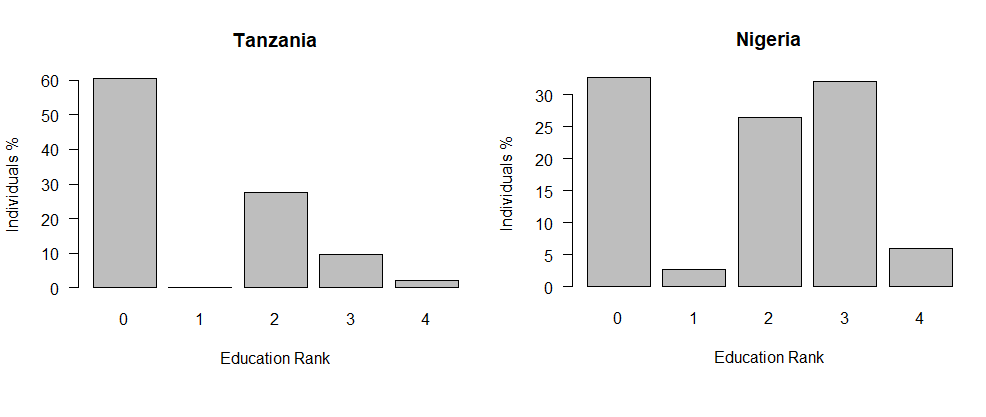
\includegraphics[width=6in]{subchapters/figures/tnz_ngr_educranks2014-2015}
\par\end{centering}
\caption{\label{fig:HistEducationRanks}Education ranks for populations in
Tanzania Nigeria (see Tables \ref{education_rank_tnz} and \ref{education_rank_ngr}
for rank classification)}
\end{figure}

\begin{figure}
\begin{centering}
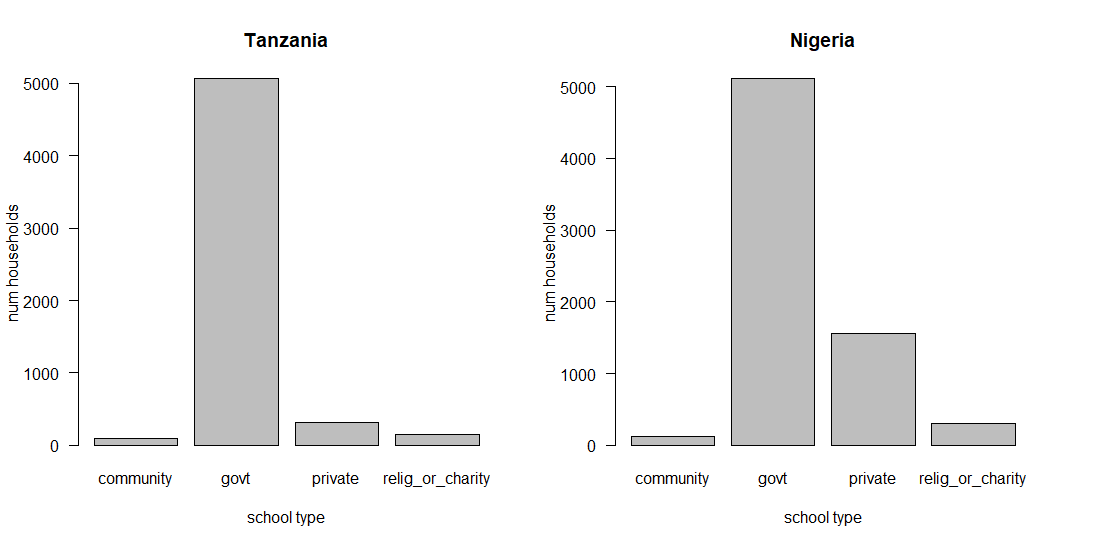
\includegraphics[width=6in]{subchapters/figures/tnz_ngr_schooltype2012}
\par\end{centering}
\caption{\label{fig:BarChartSchoolTypes}School types for non-adult population
in Tanzania and Nigeria}
\end{figure}

\begin{figure}
\begin{centering}
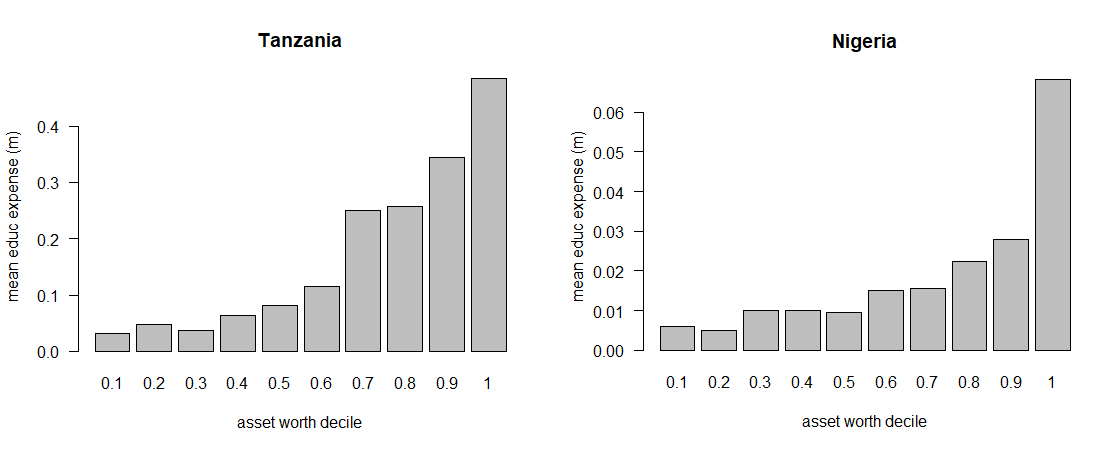
\includegraphics[width=6in]{subchapters/figures/tnz_ngr_toteducexpense2012}
\par\end{centering}
\caption{\label{fig:BarChartEducationbyAssetDeciles}Educational expenses averages
over deciles of asset worth in in Tanzania and Nigeria}
\end{figure}

% Getting rural vs urban average expenditures 
% ddply(tn$df2012 [,c("hhid2012","toteducexpense","isrural")],.(isrural),summarise,toteducexpense=mean(toteducexpense))
% Getting children's education-rank averages
% ced <- merge(unique(subset(o2012,age<18  & !is.na(highest_educ))[c("hhid","education_rank")]),unique(plyr::rename(tn$df2012,c("hhid2012"="hhid"))[,c("hhid","toteducexpense")]))
% ddply(ced,.(education_rank),summarise,toteducexpense2=mean(toteducexpense), n=length(toteducexpense))

\noindent

Considering the overall distribution of education expenses, we see
that the urban residents spend much higher on education than the rural
residents in both the economies. The urban residents spend 2.34 times
more than rural residents in Nigeria whereas they spend 2.8 times
more in Tanzania. The secondary education appears to get much costlier
in Tanzania since the mean education expenditure for tertiary education
(rank 3) is almost double that of the expenditure on secondary education
(rank 2) in Tanzania. In Nigeria, these expenditures rise by about
54\%. The educational expenses do not seem to rise much with asset
disparities in Nigeria - whereas they seem to be more unequally distributed
in Tanzania (see Figure \ref{fig:BarChartEducationbyAssetDeciles})\footnote{Despite the uniformity in LSMS data fields corresponding to education
expenses, the collection methodology may not be the same across all
the countries. This is evident from the much lower educational expenses
in Nigeria than in Tanzania (see Table \ref{tab:Summary-Stats}).
Our comparison of the two economies (Tanzania and Nigeria) therefore
does not rely on the measurement of educational expenses relative
to one another.}. Comparing education levels of the household heads, we see that the
average-education rank of the household heads in Tanzania (1.8) is
lower than that in Nigeria(1.9). We also see that the role of private
education is much higher in Nigeria (see Figure \ref{fig:BarChartSchoolTypes}).

\begin{table}[h] \centering

\resizebox{6in}{!}{
\begin{tabular}{>{\raggedright}p{1.4in}|>{\raggedleft}p{0.6in}|>{\raggedleft}p{.6in}|>{\raggedleft}p{.6in}|>{\raggedleft}p{0.6in}|>{\raggedleft}p{0.6in}|>{\raggedleft}p{0.6in}   } 

\tabularnewline            & \multicolumn{2}{c}{\emph{Tanzania}}  & &   \multicolumn{2}{c}{\emph{Nigeria}} \tabularnewline 
\hline  
Variable & $mean_{tnz}$   & $median_{tnz}$  & $stdev_{tnz}$    & $mean_{ngr}$ & $median_{ngr}$  & $stdev_{ngr}$ \tabularnewline \hline 
\texttt{w\_educ}  & 0.04 & 0.01 & 0.08 & 0.04 & 0 & 0.1 \tabularnewline \hline   
\texttt{log\_educ}   & 7.77 & 10.49 & 5.46 & 3.97 & 0 & 4.94 \tabularnewline \hline   
\texttt{\small{}ln\_tot\_exp} & 14.39 & 14.48 & 0.83 & 12.42 & 12.45 & 0.72\tabularnewline \hline  
\texttt{\small{}ln\_tot\_assets} & 12.96 & 12.76 & 1.93 & 10.93 & 11 & 1.35 \tabularnewline \hline  
\texttt{\small{}assetdensity}     & 14.9 & 14.8 & 1.13 & 11.43 & 11.42 & 0.74 \tabularnewline \hline 
\texttt{\small{}assetdensity\_educ} & 14.71 & 14.62 & 1.4 & 11.42 & 11.49 & 0.83 \tabularnewline \hline  
\texttt{\small{}assetdensity\_agri} & 14.79 & 14.82 & 1.23 & 11.36 & 11.39 & 0.84 \tabularnewline \hline  
\texttt{\small{}log\_mean\_cost\_ne} & 12.9 & 12.97 & 0.53 & 10.85 & 10.86 & 0.53 \tabularnewline \hline   
\texttt{\small{}rural\_wards} & 0.66 & 0.78 & 0.33 & 0.71 & 1 & 0.41 \tabularnewline \hline   
\texttt{secondary\_schools} & 4.56 & 2 & 7.59 & 1.22 & 1 & 0.52 \tabularnewline \hline   
\texttt{educpriv} & 0.06 & 0 & 0.23 & 0.19 & 0 & 0.39 \tabularnewline \hline   
\texttt{is\_primaryage} & 0.63 & 1 & 0.48 & 0.76 & 1 & 0.43 \tabularnewline \hline   
\texttt{is\_secondaryage}  & 0.58 & 1 & 0.49 & 0.61 & 1 & 0.49 \tabularnewline \hline   
\texttt{is\_tertiaryage} & 0.45 & 0 & 0.5 & 0.4 & 0 & 0.49  \tabularnewline \hline   
\texttt{\small{}agri} & 0.66 & 1 & 0.47 & 0.51 & 1 & 0.5 \tabularnewline \hline   
\texttt{\small{}highesteduc } &1.21 & 1 & 1.06 & 1.53 & 2 & 1.47 \tabularnewline \hline   
\texttt{\small{}numchild} &3.05 & 3 & 2.03 & 3.55 & 3 & 2.16 \tabularnewline \hline   
\texttt{religion}  &  &  &  & 1.5 & 1 & 0.52 \tabularnewline \hline   
\texttt{has\_english}  & 0.36 & 0 & 0.48 &  &  &
\end{tabular} }
\caption{\label{tab:Summary-Stats}Summary Statistics for Variables in Tables \ref{tab:Dependent-Variables} and \ref{tab:Control-Variables}}
\end{table}

Using the average, median and standard deviation values variables
listed in Tables \ref{tab:Dependent-Variables} and \ref{tab:Control-Variables})
that are shown in Table \ref{tab:Summary-Stats}, we note that the
measures for average budget shares (\texttt{w\_educ}) as well as educational
expenses (\texttt{ln\_tot\_exp}) are not dissimilar in both the economies.
The average number of children in households that are of an age appropriate
for primary, secondary or tertiary education are not far from each
other either (see values for \texttt{is\_primaryage} , \texttt{is\_secondaryage}
and \texttt{is\_tertiaryage} in Table \ref{tab:Summary-Stats}). A
clear difference between Tanzania and Nigeria - however - is that
of standard-deviation in asset density (\texttt{assetdensity}) - which
is higher for Tanzania. Further, the predominance of agricultural
occupations (see stdev values for \texttt{agri}) is higher for Tanzania
as well.

It is worth pointing that barring such broad observations, the LSMS
data used in our analyses may not permit a cross country comparison
for education expenses in a much finer detail. One reason is simply
that the distribution of savings, income and employment opportunities
is disparate in the two economies. The other reason is that there
is also a difference in sizes or granularity of district classifications
in the two economies. More specifically, the sizes of districts in
Tanzania seem much larger (particularly in the rural parts) than in
Nigeria. This is why the per-district density of secondary education
facilities - which we measure with the variable \texttt{secondary\_schools}
- is reported lower in Nigeria (see values corresponding to \texttt{secondary\_schools}
in Table \ref{tab:Summary-Stats}) - while the education levels of
the consumer populations remains higher in Nigeria (see highest\_educ
in Table \ref{tab:Summary-Stats}). The ruralness of districts - measured
as number of wards declared as rural in a district (i.e. the variable
\texttt{rural\_wards}) - does not seem affected by this disparity
in sizes as much (compare the values for \texttt{rural\_wards} in
Table \ref{tab:Summary-Stats}) - since a rural-urban classification
that declares boundaries of a district based on areas surrounding
an urban (or semi-urban) centre tends to bring a uniformity to the
number of rural wards in a district.

It is worth emphasising that the overall distribution of assets (durable
goods stocks) in the two countries is disparate - as is clear with
a direct comparison of asset values. Contrasting the Lorenz curves
for total non-durable expenditure and total assets in the Figure \ref{fig:LorenzCurves}
for in Nigeria and Tanzania, we note that distribution of assets is
more sparse in Tanzania even though the overall expenditure appears
similarly distributed in the two countries.

A geographical distribution of assets further details that higher-income
occupations are far fewer in the hinterland and the southern regions
of Tanzania (see Figure \ref{fig:occupations_r_tn-1} ) - relative
to the eastern and coastal regions that seem largely urban. The disparities
in occupations are less in Nigeria (see Figure \ref{fig:occupations_r_ngr}
).

\begin{figure}[h]
\begin{centering}
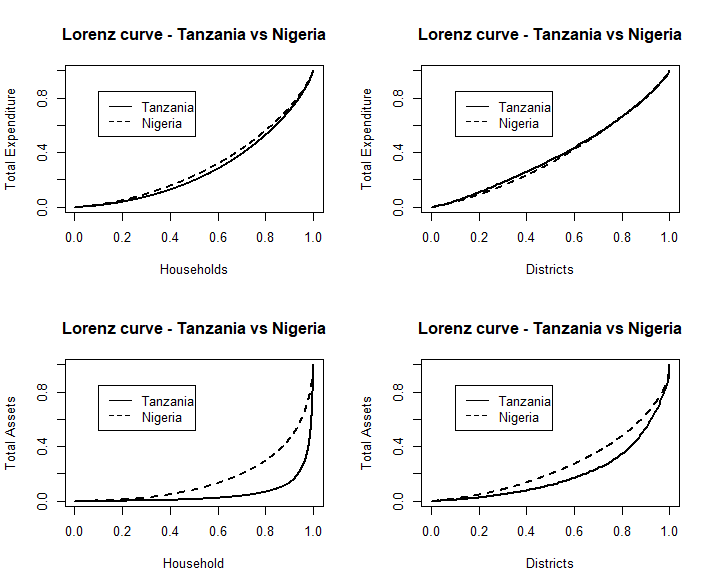
\includegraphics[width=6in]{subchapters/figures/tnz_ngr_lorenz_curves_assets_logx_district_individual}
\par\end{centering}
\caption{\label{fig:LorenzCurves}Inequality in assets and non-durable expenditure
across households and districts}
\end{figure}

\onecolumn

\begin{figure}[h]
\begin{centering}
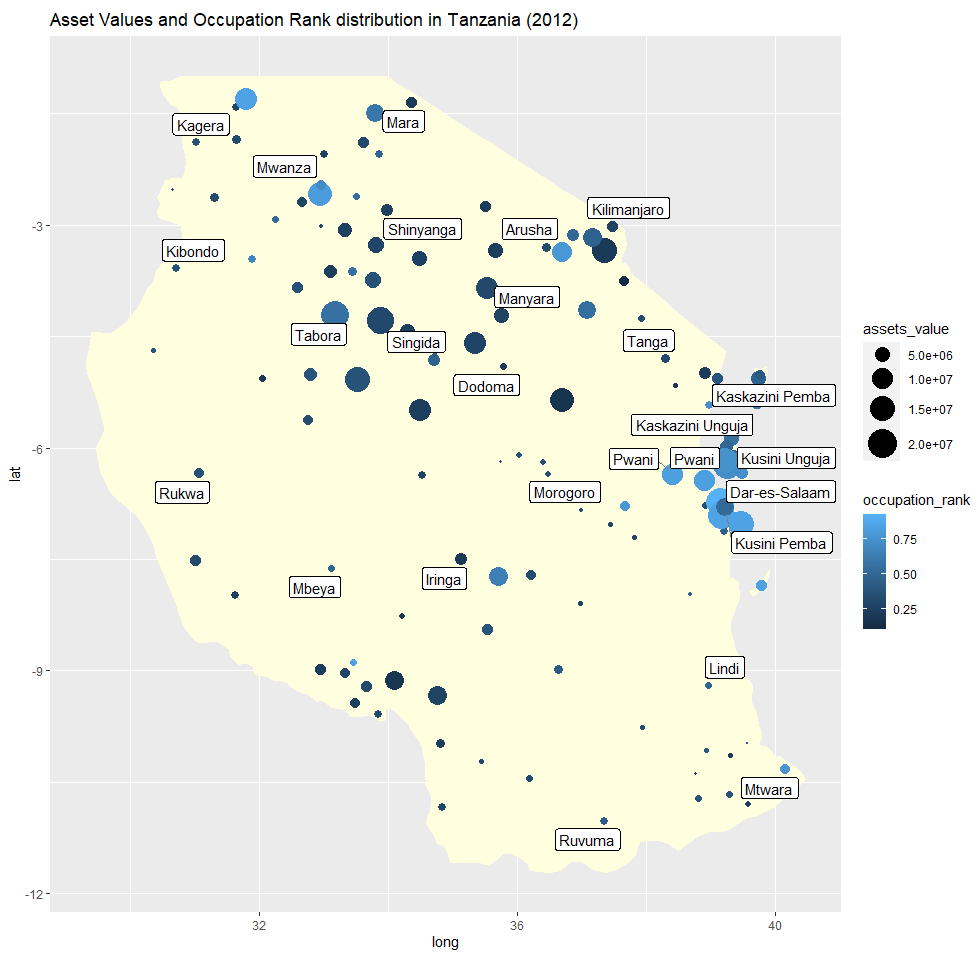
\includegraphics[width=5in]{subchapters/tnz_assets_occuprank_distribution_2012}
\par\end{centering}
\caption{\label{fig:occupations_r_tn-1}Occupations and consumer-owned assets
in Tanzania}
\end{figure}

\begin{figure}[h]
\begin{centering}
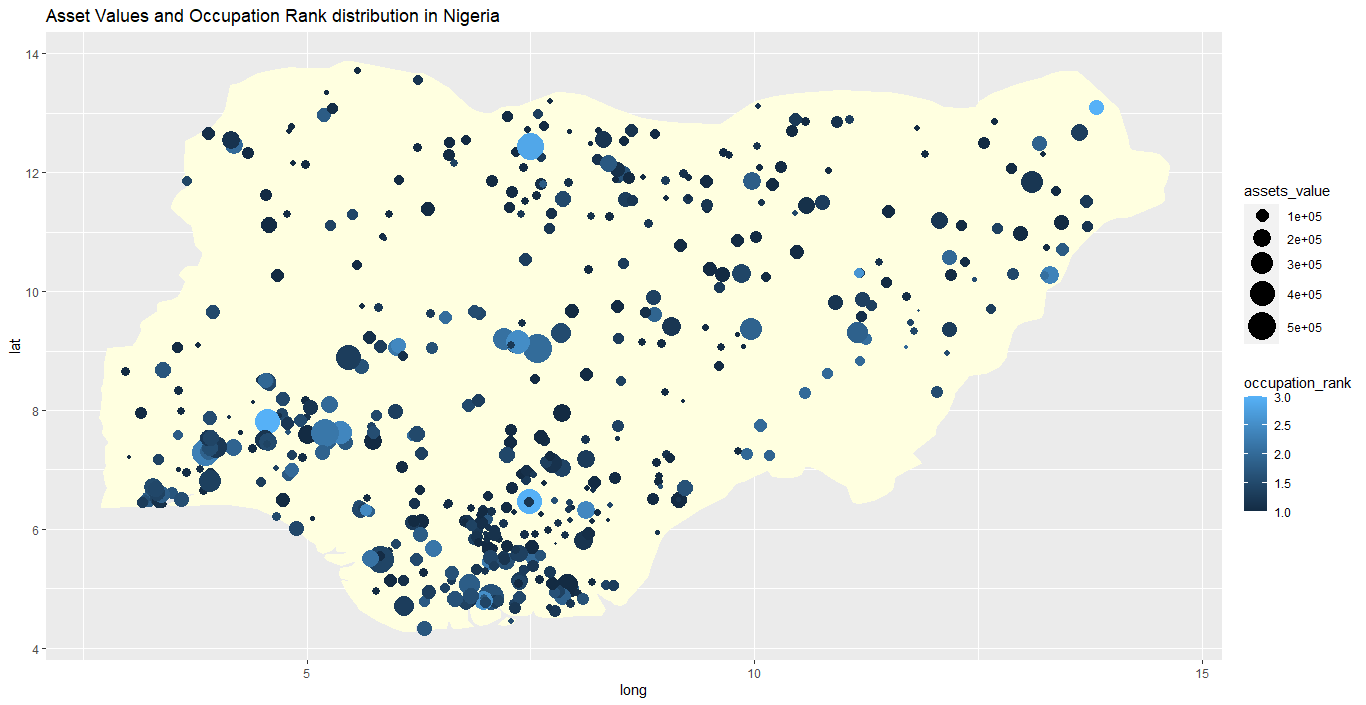
\includegraphics[width=6.5in]{subchapters/ngr_occup_2012}
\par\end{centering}
\caption{\label{fig:occupations_r_ngr}Occupations and consumer-owned assets
in Nigeria}
\end{figure}

Note that the occupation ranks shown in Figures \ref{fig:occupations_r_tn-1}
(Tanzania) and Figure \ref{fig:occupations_r_ngr} (Nigeria) are based
on the standardisation of various occupations in Tanzania and Nigeria.
Since the range of occupations in the surveys from Tanzania and Nigeria
is varied, the different occupations in the survey for Tanzania and
Nigeria have been standardised into occupation ranks (ranging from
0 to 3) based on the data on income derived from the occupations in
the survey so that a higher occupation rank represents an occupation
that provides higher income. The reason why the income itself is not
shown in the plots is that the data on income is far sparser than
the recall of assets and the reporting of occupations in surveys from
both the economies\footnote{It is not uncommon for the empirical studies in SSA to have the data
on occupation or education proxy the income differences (Alesina et
al.\cite{AlesinaMobilityAfrica2019}). The primary reason for this
is the sparsity of income data - a problem that may be further aggravated
because of a large informal sectors in the economies.}. The mapping from specific occupations to the occupation-ranks for
Tanzania and Nigeria is shown in Table \ref{occupation_rank_tn} and
\ref{occupation_rank_ngr} (respectively). A higher occupation rank
represents occupations that bring higher income. As described in Section
\ref{sec:Data-1}, the education levels are also mapped to education
ranks denoting primary, secondary and higher education (see Table
\ref{education_rank_tnz} for Tanzania and Table \ref{education_rank_ngr}
for Nigeria in the Appendix). A higher education rank corresponds
to a higher education level.

While we undertake a more detailed view on education expenses in the
Section \ref{subsec:Results}, the key observation from the data is
that the disparities in income and durable goods are more localised
in Nigeria while they are more extreme across wider geographical regions
in Tanzania. More specifically, despite the southern areas of Nigeria
having more higher-paid occupations and a higher expenditure on non-durable
expenditure overall (see Figure \ref{fig:occupations_r_ngr}), the
disparity in durable-goods ownership across regions is not as extreme
as in Tanzania. The particular interpretation of urbanisation is used
to explain the implications of this non-uniformity on consumption
and educational expenses in Section \ref{subsec:Results}.

% Lorenz curve plots
%plot(Lc(exp(ng$df2015$logx)))
% for individual totexp
%lorenz_curve(dat_a = exp(tn2012$logx),dat_b = exp(ng$df2012$logx),dat_a_name = "Tanzania",dat_b_name = "Nigeria",xlab = "Households",ylab = "Total Expenditure",use_cex = 1.)
% for district level totexp
%lorenz_curve(dat_a = exp(district_means(dat=tn2012,hhid_col = "hhid2012",field_type = "logx")$mean_logx),dat_b = exp(district_means(dat=ng$df2012,hhid_col = "hhid",field_type = "logx")$mean_logx),dat_a_name = "Tanzania",dat_b_name = "Nigeria",xlab = "Districts",ylab = "Total Expenditure",use_cex = 1.)
% for district level assets
%lorenz_curve(dat_a = exp(district_means(dat=tn2012,hhid_col = "hhid2012",field_type = "logA")$mean_logA),dat_b = exp(district_means(dat=ng$df2012,hhid_col = "hhid",field_type = "logA")$mean_logA),dat_a_name = "Tanzania",dat_b_name = "Nigeria",xlab = "Districts",ylab = "Total Assets",use_cex = 1.)
% For individual assets
%lorenz_curve(dat_a = exp(tn2012$logA),dat_b = exp(ng$df2012$logA),dat_a_name = "Tanzania",dat_b_name = "Nigeria",xlab = "Household",ylab = "Total Assets",use_cex = 1.)


\subsection{\label{subsec:Results}Results}

% We don't have panel information for 2012-2014 (for Tanzania). So we won't be using panel data. Pseudo-panel is a possibility but not considered.

\noindent

The two dependent variables we use in the estimation described in
Section \ref{sec:Econometric-Method} (see Equation \ref{eq:budgetshr_estimation})
are the budget shares for educational expenses (\texttt{$w_{educ}$})
and total expenditures (\texttt{$log(x_{educ})$}) . These dependent
variables are listed in Table \ref{tab:Dependent-Variables-1} while
controls used for the estimation are listed in Table \ref{tab:Control-Variables}.

%Variables : {wealth,wealth-conc/ruralwards,secondary_schools,occupation, parental education, language-religion, age, numchild, educpriv}

The two main explanatory variables used in the study are the the logarithm
of total expenditure \texttt{ln\_tot\_exp} and the urbanisation levels
(measured as wealth-concentration \texttt{assetdensity}). As discussed
before, an alternative formulation is also specified for comparison
- where the two explanatory variables are the logarithm of total assets
value (\texttt{ln\_tot\_assets}) and the urban/rural indicators (\texttt{rural\_wards}).
The physical access to education (i.e. \texttt{secondary\_schools})
is an important control in both the formulations. Other controls used
in the comparison are the indicator for an agrarian occupation \texttt{agri}
($\Omega$), the paternal education level \texttt{highesteduc} ($\Gamma^{*}$),
the religion and language indicators ( \texttt{religion} $\chi$ used
only for Nigeria indicated by 1 for Christianity, 2 for Islam, 3 for
Traditional, 4 for other - and English-speaking ability i.e. the variable
\texttt{has\_english $\xi$ }indicating the ability to speak English
used only for Tanzania), the access to private education (\texttt{educpriv}
or $\pi$), the number of children ( \texttt{numchild} or $h$) and
their ages \texttt{is\_primaryage} ($\mu_{1}$),\texttt{ is\_secondaryage}
($\mu_{2}$)\texttt{, is\_tertiaryage} ($\mu_{3})$ indicating if
they are eligible (due to age) for primary, secondary or tertiary
education (respectively) and the non-durable consumption prices \texttt{\small{}(log\_mean\_cost\_ne}
$p_{ne}$). All of the controls remain the same for the main as well
as alternative formulation. Recall that the non-durable consumption
prices $p_{ne}$ (see Section \ref{sec:Data-1}) - interpreted as
the cost of living in the vicinity - is measured as \texttt{\small{}log\_mean\_cost\_ne}
- the logarithm of average consumption excluding the asset-related
costs in the consumer's vicinity. Notice that the factor variables
are prefixed with respective values \texttt{1.} , \texttt{2.} etc.
in the results.

Of the control variables and explanatory variables discussed above,
some are observed at the household level while others are observed
at the level of the consumer's district. The logarithm of total expenditure
\texttt{ln\_tot\_exp} and of the total assets-owned \texttt{ln\_tot\_assets}
are observed at the level of the household. Similarly, the agricultural-occupation
factor variable \texttt{agri} (indicating whether the household head
is employed in agriculture related occupation or not), the number
of children in the household \texttt{numchild}, the childrens' ages
factor variables \texttt{is\_primaryage} ,\texttt{ is\_secondaryage}
and \texttt{is\_tertiaryage} ), the private education factor variable
\texttt{educpriv}, the highest education rank \texttt{highesteduc}
corresponding to the paternal generations (father-relationship) in
a household, the ability to speak English \texttt{has\_english} (used
only for Tanzania) and the household religion \texttt{religion} (used
only for Nigeria) are all observed for a household. The variables
observed at the district (or 6-$km$ vicinity) are the number of wards
with an accessible (within 6-km distance) secondary-schools (\texttt{secondary\_schools}),
the rural wards (\texttt{\small{}rural\_wards}) in a district, the
respective measures of the wealth-concentration \texttt{\small{}assetdensity}
and the logarithm of the per-head cost non-durable consumption \texttt{\small{}log\_mean\_cost\_ne}
.

To reiterate, a significant number of household units in both the
economies are made up of joint families where the reported educational
expenses correspond to the grandchildren of the household head (HH).
The education level of the HH would thus point to the penultimate
generation for households where HH has grandchildren and the previous
generation for younger households where HH has young children. To
resolve this disparity, we avoid using the education rank of the HH
and instead use the highest education rank in the generation of the
students' parents \footnote{Only relations with the household head are reported in the survey.
Thus, there is no direct way of locating the parent of a child except
through the relation with the household-head.} \texttt{\small{}highesteduc} instead. The paternal educational level
\texttt{\small{}highesteduc} suffices for our analysis of expenditure
spent over all the children in the household (rather than how education
budget is distributed among the male/female children). As mentioned
in the Section \ref{sec:Econometric-Method}, the households with
no children are ignored in the analysis. Nearly 22\% of households
in the Nigeria and 15 \% of households in Tanzania are thus excluded
from our comparison.

Notice also that the age-variables \texttt{is\_primaryage}, \texttt{is\_secondaryage},
\texttt{is\_tertiaryage} for attendance of primary, secondary and
tertiary education have been used in the analysis to get around the
unavailability of the current-education level of the household member
in the Nigerian LSMS survey data. Instead, we use a combination of
the indicator variable telling whether a household member is in school
or not (available in the surveys for both Tanzania and Nigeria) and
the mean school attendance ages to define variables \texttt{is\_primaryage},
\texttt{is\_secondaryage} and \texttt{is\_tertiaryage} that indicate
whether there is a household member of an age appropriate for attending
primary, secondary and tertiary education levels (respectively).

% For Nigeria: length(unique(subset(ng$df2015,toteducexpense==0)$hhid))/length(unique(ng$df2015$hhid)) = .67493
% For Tanzania: length(unique(subset(tn$df2014,toteducexpense==0)$hhid))/length(unique(tn$df2014$hhid)) = .4215

The results from the a tobit estimation for educational expenses (\texttt{$w_{educ}$})
and total expenditures (\texttt{$log(x_{educ})$}) with wealth-concentration
\texttt{assetdensity} as one of the controls are shown in Table \ref{tabTNZNGR_r}
for both Tanzania and Nigeria. The tobit uses a lower limit of zero
given a number of houses have no expenditure on education. A zero
expenditure is reported for nearly 65\% households in the survey from
Nigeria (2015) and 43\% households in the survey from Tanzania (2014).
This suggests that either the education expenses are recorded in more
detail in Tanzania or that a certain basic level of expenses is not
considered in the survey for Nigeria. The particular disparity also
limits our ability to compare educational expenses relative to one
another for the two economies. A discussion on the cross-section results
from the latest available years 2014 for Tanzania and 2015 for Nigeria
follows in Section \ref{subsec:Discussion} (see Table \ref{tabTNZNGR_r}).
The results from the alternative formulation - where the main explanatory
variables are the logarithm of total assets value \texttt{\small{}ln\_tot\_assets}
(used in place of household total expenditure) and the ruralness-score
\texttt{\small{}rural\_wards }derived from the survey's classification
of rural and urban areas (used in place of wealth concentration \texttt{\small{}assetdensity})
- are also discussed in \ref{subsec:Discussion} (see Table \ref{tabTNZNGR_urbanrural}).

\newpage

\subsection{\label{subsec:Discussion}Discussion}

%[secondary_schools effect]
%For Nigeria, the secondary-schools were split into community and government schools - whose sum turns out to be less than the schools recorded in the previous year. This seems to the cause of some disparity in the two years - even though the effect of this variable does not appear as significant as wealth.
% NGR:
% a<- merge(ddply(unique(subset(ng$df2012[,c("region","district","secondary_schools")],!is.na(secondary_schools))),.(region),summarise,n=sum(secondary_schools)), ddply(unique(subset(ng$df2015[,c("region","district","secondary_schools")],!is.na(secondary_schools))),.(region),summarise,n=sum(secondary_schools)), by =c("region"))
% b<- merge(ddply(unique(subset(tn$df2012[,c("region","district","secondary_schools")],!is.na(secondary_schools))),.(region),summarise,n=sum(secondary_schools)), ddply(unique(subset(tn$df2014[,c("region","district","secondary_schools")],!is.na(secondary_schools))),.(region),summarise,n=sum(secondary_schools)), by =c("region"))
%[secondary_schools effect]


\noindent

%[ln_tot_exp effect on budget share]

\subsubsection*{Results with \texttt{$w_{educ}$ }as the dependent variable}

\noindent

The coefficient of the total expenditure ( \texttt{ln\_tot\_exp)}
in Table \ref{tabTNZNGR_r} for $w_{educ}$ as the dependent variable
suggest that an increase in the total expenditure ( \texttt{ln\_tot\_exp)}
causes a decrease in the budget share on education \texttt{($w_{educ}$}
) for both Tanzania and Nigeria. This seems largely due to the educational
expenses forming a higher proportion of the total expenditure for
poorer households - since the education expenditures $log(x_{educ})$
do seem to rise with the increase in total expenditure ( \texttt{ln\_tot\_exp)}
in Tanzania (see coefficient of \texttt{ln\_tot\_exp} under columns
for $log(x_{educ})$ in Table \ref{tabTNZNGR_r} ). The effect of
non-durable consumption prices (\texttt{log\_mean\_cost\_ne} ) is
weak on education-budget share \texttt{$w_{educ}$} for both the economies
(see coefficient of \texttt{log\_mean\_cost\_ne} under $w_{educ}$
in Table \ref{tabTNZNGR_r}) . Thus while urbanisation must raise
the prices of non-durable expenditure \texttt{log\_mean\_cost\_ne},
the disparity in budget shares does not appear to be due to higher
cost of living (non-durable consumption) alone. In other words, the
expenditure on education is necessitated despite the lower or higher
cost of living across the regions in both the economies.

%[r - w_educ]

Instead, we see a strong and positive effect of wealth concentration
( \texttt{assetdensity} ) towards educational budget shares (\texttt{$w_{educ}$})
in both the countries in Table \ref{tabTNZNGR_r} (see coefficients
of \texttt{assetdensity} under $w_{educ}$ in Table \ref{tabTNZNGR_r}
). This is an indication of the regional disparities in the economies.
More particularly, the differences in density of assets indicate the
level of urbanisation that have a strong effect on education expenses
- despite controlling for the effect of availability of secondary-school
education. While absence of educational facilities must clearly suppress
education expenses in a region, the positive effect of assets-density
after controlling for availability of education facilities also suggests
relevance of certain environmental factors that contribute to education
- such as a competition towards higher income social positions or
presence of occupations requiring higher levels of education - factors
with an important role after the availability of educational facilities
has been considered.

The effects of household total expenditure are - however - relevant
for private education - which is limited to the wealthier households
in both the economies regardless of wealth-concentration ( \texttt{assetdensity}
). While a higher proportion of young population seems to be in private
schools in Nigeria (see Figure \ref{fig:BarChartSchoolTypes}), private
education is slightly higher in budget share in Tanzania as the privately-educated
households in Nigeria show higher budget shares \texttt{$w_{educ}$
}(see coefficients of \texttt{educpriv} under $w_{educ}$ for the
two countries in Table \ref{tabTNZNGR_r} ). However, since private
education only accounts for a minority of the population in both the
economies (see Figure \ref{fig:BarChartSchoolTypes}), the role of
access to either or private or government secondary school i.e. we
focus on the variable \texttt{secondary\_schools} for our comparison
of education expenses in the two countries.

Viewing the effect of the variable \texttt{secondary\_schools} on
education budget shares \texttt{$w_{educ}$}, we see a far stronger
effect of \texttt{secondary\_schools} for Tanzania (compare the coefficients
for secondary-school $s$ i.e. \texttt{secondary\_schools }in Tables
\ref{tabTNZNGR_r}) . It also seems that the consumers are more likely
to spend on primary education in Tanzania - as the access to secondary
and tertiary-education remains much lower (this is further elaborated
in discussion below of the results using education expenditure \texttt{$log(x_{educ})$}
as dependent variable).

The results from the alternative formulation using urban-rural indicators
suggest a particular limitation of the use of urban-rural indicators
from the survey. More specifically, the coefficients of rural-wards
\texttt{(rural\_wards}) for education budget shares \texttt{$w_{educ}$}
are negative and significant for Tanzania in Table \ref{tabTNZNGR_urbanrural}.
However, the inference of a higher expenditure on education - when
using urban-rural indicators - by the rural residents in Nigeria (see
significance of rural-wards \texttt{rural\_wards }in Table \ref{tabTNZNGR_urbanrural}
) may be improper as it ignores the fact that the wards identified
as rural in Nigeria may not be as rural as those identified as rural
in Tanzania. This is confirmed with the weaker role of wealth i.e.
assets-worth-logarithm ( \texttt{ln\_tot\_assets} in Table \ref{tabTNZNGR_urbanrural})
and a strong role for wealth-concentration (\texttt{assetdensity}
in Table \ref{tabTNZNGR_r}) for Nigeria in the alternative formulation.
Compared with urban-rural indicators, the wealth-concentration \texttt{assetdensity}
seems to provide us a more clear-cut and standardised interpretation
of urbanisation in the two economies.

%[log(x_educ)]

\subsubsection*{Results with \texttt{$log(x_{educ})$ }as the dependent variable}

\noindent

Comparing the results with education-expenditure logarithm \texttt{$log(x_{educ})$
}as the dependent variable, we see that the education expenditures
rise with the increase in total expenditure logarithm (\texttt{ln\_tot\_exp})
for Tanzania but the effect of total expenditure \texttt{\small{}ln\_tot\_exp}
(in Table \ref{tabTNZNGR_r}) is not significant for Nigeria. While
the higher expenditure on education measured through total education
expenditure logarithm \texttt{$log(x_{educ})$} does seem to respond
to the prices of non-durable consumption \texttt{log\_mean\_cost\_ne}
in Tanzania (see coefficient of \texttt{log\_mean\_cost\_ne} under
column $log(x_{educ})$ in Table \ref{tabTNZNGR_r}), the effect of
non-durable consumption prices \texttt{log\_mean\_cost\_ne} remains
weak on education-budget share \texttt{$w_{educ}$} for both the economies
(see above discussion using budget share \texttt{$w_{educ}$} as the
dependent variable). We also see that the educational expenditure
$log(x_{educ})$ rises with the second explanatory variable i.e. the
wealth concentration ( \texttt{assetdensity} ) for Nigeria while the
effect of wealth concentration \texttt{assetdensity} is insignificant
for Tanzania (compare coefficients for \texttt{assetdensity} against
both the countries in Table \ref{tabTNZNGR_r} under columns for $log(x_{educ})$
). In the alternative formulation where urbanisation is measured with
the ruralness score ( \texttt{rural\_wards} ), the ruralness score
corresponds to a rise in educational expenditure \texttt{$log(x_{educ})$}
for Nigeria and a drop in educational expenditure \texttt{$log(x_{educ})$
}for Tanzania (see coefficients for \texttt{rural\_wards} under columns
for \texttt{$log(x_{educ})$} in Table \ref{tabTNZNGR_urbanrural}).
The disparity in the role of \texttt{rural\_wards} is however also
due to differences in the extent to which density of educational institutions
depends on \texttt{rural\_wards} in the respective countries.

Continuing with the comparison of results with education-expenditure
$log(x_{educ})$ as the dependent variable, we see that private-education
indicator variable \texttt{educpriv} is insignificant for Nigeria
(see Table \ref{tabTNZNGR_r} ). The education expenses in Nigeria
therefore depend less often on whether education is provided through
private educational institutions or not. The results also indicate
lower access to secondary and tertiary-education in Tanzania (see
coefficients of secondary-school-age\texttt{ is\_secondaryage} and
tertiary-school-age \texttt{is\_tertiaryage} in regression results
with education expenditure logarithm $log(x_{educ})$ as the dependent
variable in Table \ref{tabTNZNGR_r}). In the alternative formulation,
the results with education expenditure logarithm \texttt{$log(x_{educ})$
}as dependent variable in Tables \ref{tabTNZNGR_urbanrural} show
the role of secondary-school access \texttt{secondary\_schools} to
be stronger for Nigeria when taking wealth i.e. total assets-worth
logarithm \texttt{ln\_tot\_assets }into account. The wealth effect
thus seems stronger than access in both the economies but is weaker
for Nigeria where the enrollment into secondary and tertiary education
is higher - regardless of the differences in long-term intergenerational
wealth (measured with logarithm of assets-worth \texttt{ln\_tot\_assets}).
The decomposed view of expenses on education in terms of secondary
and primary education level further clarifies this observation - reflecting
the far lower access to secondary education in Tanzania.

\subsubsection*{Other controls}

\noindent

The role of the number of children (\texttt{numchild}) also seems
stronger in Tanzania than in Nigeria - but the effect is likely due
the education expenses primarily driven by the primary education levels
in Tanzania (as well as a higher percentage of households reporting
no education expenditure in the survey from Nigeria). Another consequence
of most households spending on primary education alone is that the
agrarian households appear as spending higher on education after considering
the wealth-concentration among households with the same educational-status.
The education expenditure is higher for agrarian households in Tanzania
after taking into account their poor educational status (see coefficients
of agrarian-occupation-indicator \texttt{1.is\_agri} in Table \ref{tabTNZNGR_r}
under column for the education-expenditure-logarithm \texttt{$log(x_{educ})$}
dependent variable).

The wealth effects in Tanzania overall seem stronger, but they ought
to be considered in light of the much lower expenditure on secondary
(and higher) education and higher disparity in asset-ownership (even
after taking into account the lower urbanisation levels) in Tanzania.
The significance of logarithm of assets-worth ( \texttt{ln\_tot\_assets
}in Table \ref{tabTNZNGR_urbanrural}) does indicate a general trend
where those with higher inter-generational wealth and in urban areas
(see significance of \texttt{ln\_tot\_assets }and \texttt{rural\_wards}
in Table \ref{tabTNZNGR_urbanrural} for Tanzania $log(x_{educ})$
as dependent variable) are far more likely to avail the education
facilities, but a higher dependence on industrial output in Nigeria
also seems to have contributed to a higher demand for secondary and
tertiary education in the economy overall ( compare with significance
of \texttt{ln\_tot\_assets }, \texttt{1.is\_secondaryage} and \texttt{rural\_wards}
in Table \ref{tabTNZNGR_urbanrural} for Nigeria with $log(x_{educ})$
as dependent variable). Another observation - the stronger role of
father's education level in Tanzania - also seems related with these
disparities in the two economies as well. A comparison of education
expenditures across the two countries must take into account the different
stages which the two countries appear to be in terms of urbanisation
and economic development.

Finally, the role of social environment is found significant in both
the economies. The role of English language seems significant in Tanzania
- where the English-speakers spend significantly higher on education
(see coefficients of \texttt{has\_english} in Table \ref{tabTNZNGR_r}
under  $log(x_{educ})$ )\textbf{ }. In Nigeria, on the other hand,
the educational expenses are higher among households identifying as
Christian (see coefficients of\texttt{ religion} in Table \ref{tabTNZNGR_r}
under $log(x_{educ})$ ) . In both cases, the role of social characteristics
may be rather inseparable from differences in educational institutions.
In case of Tanzania, the ability to speak English is aligned with
attending educational institutions while in Nigeria, the role played
by Christian missionaries in establishment of educational institutions
may be reflected in the disparity of access to educational facilities.

\begin{table}\centering
\caption{Tanzania -Nigeria - Differences in Wealth Concentration  \label{tabTNZNGR_r}}
\resizebox{4in}{!}{
\def\sym#1{\ifmmode^{#1}\else\(^{#1}\)\fi}     
\begin{tabular} { l c c  c c }
\hline\hline       

          &\multicolumn{2}{c}{$w_{educ}$}       &\multicolumn{2}{c}{$log(x_{educ})$}  \\\cmidrule(lr){2-3}\cmidrule(lr){4-5}           &\multicolumn{1}{c}{}&\multicolumn{1}{c}{}&\multicolumn{1}{c}{}&\multicolumn{1}{c}{}\\           &\multicolumn{1}{c}{\emph{Tanzania}}&\multicolumn{1}{c}{\emph{Nigeria}}&\multicolumn{1}{c}{\emph{Tanzania}}&\multicolumn{1}{c}{\emph{Nigeria}}\\ \midrule ln\_tot\_exp      & -0.00908\sym{**} &  -0.0283\sym{***}&    1.224\sym{***}&    0.133         \\           &  (0.004)         &  (0.000)         &  (0.000)         &  (0.744)         \\ assetdensity     &  0.00488\sym{*}  &   0.0299\sym{***}&  -0.0368         &    1.497\sym{***}\\           &  (0.015)         &  (0.000)         &  (0.758)         &  (0.000)         \\ log\_mean\_cost\_ne&   0.0490         &   0.0479         &    9.165\sym{*}  &   -0.155         \\           &  (0.467)         &  (0.672)         &  (0.023)         &  (0.981)         \\ 1.agri    &  0.00735         &  0.00990         &    0.953\sym{**} &    0.574         \\           &  (0.167)         &  (0.308)         &  (0.003)         &  (0.297)         \\ 1.educpriv&   0.0756\sym{***}&   0.0475\sym{***}&    2.890\sym{***}&    0.815         \\           &  (0.000)         &  (0.000)         &  (0.000)         &  (0.197)         \\ 1.highesteduc&   0.0109\sym{*}  &   0.0829         &    0.694\sym{*}  &    5.899         \\           &  (0.030)         &  (0.301)         &  (0.021)         &  (0.202)         \\ 2.highesteduc&  0.00432         &  0.00679         &    0.366         &    0.363         \\           &  (0.711)         &  (0.585)         &  (0.598)         &  (0.607)         \\ 3.highesteduc&  0.00457         & -0.00520         &    0.473         &   -0.528         \\           &  (0.519)         &  (0.627)         &  (0.263)         &  (0.381)         \\ 4.highesteduc&   0.0250\sym{*}  &   0.0120         &    1.465\sym{*}  &    0.183         \\           &  (0.011)         &  (0.506)         &  (0.013)         &  (0.859)         \\ secondary\_schools& -0.00138\sym{***}&  0.00738         & -0.00569         &    0.384         \\           &  (0.000)         &  (0.373)         &  (0.734)         &  (0.414)         \\ 1.is\_primaryage&   0.0793\sym{***}&   0.0538\sym{***}&    8.842\sym{***}&    3.301\sym{***}\\           &  (0.000)         &  (0.000)         &  (0.000)         &  (0.000)         \\ 1.is\_secondaryage&   0.0123\sym{**} &   0.0605\sym{***}&    0.143         &    2.230\sym{***}\\           &  (0.005)         &  (0.000)         &  (0.580)         &  (0.000)         \\ 1.is\_tertiaryage&  -0.0131\sym{**} &   0.0174         &   -1.281\sym{***}&    0.931         \\           &  (0.001)         &  (0.056)         &  (0.000)         &  (0.071)         \\ 1.has\_english&   0.0584\sym{***}&                  &    2.249\sym{***}&                  \\           &  (0.000)         &                  &  (0.000)         &                  \\ numchild  &  0.00433\sym{***}& -0.00221         &    0.259\sym{***}&  -0.0499         \\           &  (0.000)         &  (0.360)         &  (0.000)         &  (0.714)         \\ 2.religion&                  &  -0.0455\sym{***}&                  &   -2.043\sym{***}\\           &                  &  (0.000)         &                  &  (0.000)         \\ 3.religion&                  &  -0.0632         &                  &   -2.160         \\           &                  &  (0.170)         &                  &  (0.396)         \\ \_cons    &   -0.151         &   -0.231         &   -41.97\sym{***}&   -22.99         \\           &  (0.346)         &  (0.352)         &  (0.000)         &  (0.103)         \\ \midrule sigma     &                  &                  &                  &                  \\ \_cons    &   0.0876\sym{***}&    0.173\sym{***}&    5.361\sym{***}&    9.969\sym{***}\\           &  (0.000)         &  (0.000)         &  (0.000)         &  (0.000)         \\ \midrule \(N\)     &     2410         &     2192         &     2410         &     2192         \\ 

\end{tabular}
}
\end{table}

\begin{table}\centering
\caption{Tanzania-Nigeria - Urban-Rural Differences \label{tabTNZNGR_urbanrural}}
\resizebox{4in}{!}{
\def\sym#1{\ifmmode^{#1}\else\(^{#1}\)\fi}     
\begin{tabular} { l c c  c c }
\hline\hline       

          &\multicolumn{2}{c}{$w_{educ}$}       &\multicolumn{2}{c}{$log(x_{educ})$}  \\\cmidrule(lr){2-3}\cmidrule(lr){4-5}           &\multicolumn{1}{c}{}&\multicolumn{1}{c}{}&\multicolumn{1}{c}{}&\multicolumn{1}{c}{}\\           &\multicolumn{1}{c}{\emph{Tanzania}}&\multicolumn{1}{c}{\emph{Nigeria}}&\multicolumn{1}{c}{\emph{Tanzania}}&\multicolumn{1}{c}{\emph{Nigeria}}\\ \midrule ln\_tot\_assets      & -0.00590\sym{***}& -0.00196         &    0.392\sym{***}&    0.363         \\           &  (0.000)         &  (0.576)         &  (0.000)         &  (0.065)         \\ log\_mean\_cost\_ne&  -0.0548         & -0.00483         &    9.559\sym{*}  &    8.263         \\           &  (0.455)         &  (0.965)         &  (0.031)         &  (0.182)         \\ 1.agri    &   0.0106\sym{*}  &  0.00507         &    0.925\sym{**} &  -0.0768         \\           &  (0.048)         &  (0.617)         &  (0.004)         &  (0.892)         \\ 1.educpriv&   0.0800\sym{***}&   0.0506\sym{***}&    2.730\sym{***}&    1.016         \\           &  (0.000)         &  (0.000)         &  (0.000)         &  (0.113)         \\ 1.highesteduc&   0.0107\sym{*}  &   0.0948         &    0.679\sym{*}  &    7.172         \\           &  (0.032)         &  (0.244)         &  (0.023)         &  (0.121)         \\ 2.highesteduc&  0.00199         &  0.00689         &    0.512         &    0.481         \\           &  (0.864)         &  (0.583)         &  (0.462)         &  (0.495)         \\ 3.highesteduc&  0.00359         & -0.00767         &    0.607         &   -0.551         \\           &  (0.608)         &  (0.478)         &  (0.149)         &  (0.361)         \\ 4.highesteduc&   0.0273\sym{**} &   0.0129         &    1.320\sym{*}  &    0.486         \\           &  (0.005)         &  (0.480)         &  (0.025)         &  (0.636)         \\ secondary\_schools& -0.00111\sym{***}&   0.0147         &  0.00265         &    0.906         \\           &  (0.000)         &  (0.085)         &  (0.875)         &  (0.058)         \\ 1.is\_primaryage&   0.0797\sym{***}&   0.0562\sym{***}&    8.812\sym{***}&    3.408\sym{***}\\           &  (0.000)         &  (0.000)         &  (0.000)         &  (0.000)         \\ 1.is\_secondaryage&   0.0129\sym{**} &   0.0593\sym{***}&    0.145         &    2.259\sym{***}\\           &  (0.003)         &  (0.000)         &  (0.572)         &  (0.000)         \\ 1.is\_tertiaryage&  -0.0121\sym{**} &   0.0139         &   -1.240\sym{***}&    0.878         \\           &  (0.003)         &  (0.132)         &  (0.000)         &  (0.088)         \\ rural\_wards&  -0.0229\sym{**} &   0.0133         &   -1.184\sym{*}  &    1.848\sym{**} \\           &  (0.007)         &  (0.291)         &  (0.021)         &  (0.009)         \\ 1.has\_english&   0.0599\sym{***}&                  &    2.436\sym{***}&                  \\           &  (0.000)         &                  &  (0.000)         &                  \\ numchild  &  0.00426\sym{***}& -0.00354         &    0.304\sym{***}&  -0.0588         \\           &  (0.000)         &  (0.143)         &  (0.000)         &  (0.662)         \\ 2.religion&                  &  -0.0445\sym{***}&                  &   -1.716\sym{**} \\           &                  &  (0.000)         &                  &  (0.003)         \\ 3.religion&                  &  -0.0725         &                  &   -2.411         \\           &                  &  (0.120)         &                  &  (0.343)         \\ \_cons    &    0.143         &   -0.103         &   -30.47\sym{**} &   -29.99\sym{*}  \\           &  (0.452)         &  (0.698)         &  (0.008)         &  (0.044)         \\ \midrule sigma     &                  &                  &                  &                  \\ \_cons    &   0.0870\sym{***}&    0.175\sym{***}&    5.357\sym{***}&    9.994\sym{***}\\           &  (0.000)         &  (0.000)         &  (0.000)         &  (0.000)         \\ \midrule \(N\)     &     2410         &     2192         &     2410         &     2192         \\ 

\end{tabular}
}
\end{table}

\bigskip{}

\begin{landscape}
\begin{table}[!htpb]\centering
\caption{Tanzania-Nigeria - around median assets-value \label{tabTNZNGR_abovebelow_median}}
\resizebox{7.5in}{!}{
\def\sym#1{\ifmmode^{#1}\else\(^{#1}\)\fi}     
\begin{tabular} { l c c  c c c c c c }
\hline\hline       

          &\multicolumn{2}{c}{$w_{educ}$}&\multicolumn{2}{c}{$log(x_{educ})$}&\multicolumn{2}{c}{$w_{educ}$}&\multicolumn{2}{c}{$log(x_{educ})$}\\\cmidrule(lr){2-3}\cmidrule(lr){4-5}\cmidrule(lr){6-7}\cmidrule(lr){8-9}           &\multicolumn{1}{c}{Above Median }&\multicolumn{1}{c}{Above Median }&\multicolumn{1}{c}{Above Median }&\multicolumn{1}{c}{Above Median }&\multicolumn{1}{c}{Below Median }&\multicolumn{1}{c}{Below Median }&\multicolumn{1}{c}{Below Median }&\multicolumn{1}{c}{Below Median }
\\           &\multicolumn{1}{c}{\emph{Tanzania}}&\multicolumn{1}{c}{\emph{Nigeria}}&\multicolumn{1}{c}{\emph{Tanzania}}&\multicolumn{1}{c}{\emph{Nigeria}}&\multicolumn{1}{c}{\emph{Tanzania}}&\multicolumn{1}{c}{\emph{Nigeria}}&\multicolumn{1}{c}{\emph{Tanzania}}&\multicolumn{1}{c}{\emph{Nigeria}}
\\ \midrule ln\_tot\_exp      & -0.00338         &  -0.0168         &    0.783\sym{**} &    0.411         &  -0.0121\sym{**} &  -0.0458\sym{***}&    1.272\sym{***}&   -0.582         \\           &  (0.483)         &  (0.113)         &  (0.005)         &  (0.511)         &  (0.006)         &  (0.000)         &  (0.000)         &  (0.321)         \\ assetdensity     &  0.00512         &   0.0321\sym{***}&   -0.160         &    1.818\sym{***}&  0.00592         &   0.0227\sym{*}  &  -0.0190         &    0.819         \\           &  (0.061)         &  (0.000)         &  (0.311)         &  (0.000)         &  (0.052)         &  (0.024)         &  (0.919)         &  (0.131)         \\ log\_mean\_cost\_ne&  -0.0900         & -0.00476         &    11.02         &   -6.579         &    0.165         &    0.100         &    7.127         &    5.568         \\           &  (0.363)         &  (0.976)         &  (0.056)         &  (0.479)         &  (0.080)         &  (0.539)         &  (0.219)         &  (0.528)         \\ 1.agri    &  0.00286         &  0.00554         &    0.758         &    0.341         &   0.0129         &   0.0157         &    1.151\sym{*}  &    0.809         \\           &  (0.671)         &  (0.665)         &  (0.052)         &  (0.650)         &  (0.139)         &  (0.294)         &  (0.031)         &  (0.314)         \\ 1.educpriv&   0.0850\sym{***}&   0.0348\sym{*}  &    3.219\sym{***}&    0.726         &   0.0527\sym{**} &   0.0711\sym{***}&    2.083         &    0.896         \\           &  (0.000)         &  (0.010)         &  (0.000)         &  (0.364)         &  (0.004)         &  (0.000)         &  (0.074)         &  (0.406)         \\ 1.highesteduc&   0.0102         &   0.0847         &    0.443         &    8.091         &   0.0118         &    0.107         &    0.850\sym{*}  &    5.336         \\           &  (0.156)         &  (0.482)         &  (0.292)         &  (0.263)         &  (0.089)         &  (0.323)         &  (0.047)         &  (0.368)         \\ 2.highesteduc&   0.0208         &  0.00761         &    0.759         &    0.178         &  -0.0235         &  0.00660         &   -0.380         &    0.618         \\           &  (0.170)         &  (0.645)         &  (0.390)         &  (0.855)         &  (0.207)         &  (0.727)         &  (0.735)         &  (0.543)         \\ 3.highesteduc&-0.000380         & -0.00517         &  -0.0789         &   -0.359         &   0.0114         & -0.00197         &    1.171         &   -0.594         \\           &  (0.967)         &  (0.711)         &  (0.882)         &  (0.661)         &  (0.310)         &  (0.906)         &  (0.092)         &  (0.508)         \\ 4.highesteduc&   0.0204         &  0.00328         &    0.796         &   -0.695         &   0.0368         &   0.0426         &    2.572\sym{*}  &    2.785         \\           &  (0.079)         &  (0.877)         &  (0.240)         &  (0.577)         &  (0.062)         &  (0.222)         &  (0.036)         &  (0.139)         \\ secondary\_schools& -0.00128\sym{***}& -0.00325         & -0.00576         &   -0.524         & -0.00161\sym{**} &   0.0230         &  0.00286         &    1.669\sym{*}  \\           &  (0.000)         &  (0.764)         &  (0.770)         &  (0.413)         &  (0.001)         &  (0.077)         &  (0.926)         &  (0.018)         \\ 1.is\_primaryage&   0.0610\sym{***}&   0.0465\sym{**} &    7.280\sym{***}&    2.766\sym{**} &    0.101\sym{***}&   0.0664\sym{***}&    10.53\sym{***}&    3.983\sym{***}\\           &  (0.000)         &  (0.003)         &  (0.000)         &  (0.003)         &  (0.000)         &  (0.000)         &  (0.000)         &  (0.000)         \\ 1.is\_secondaryage&  0.00978         &   0.0692\sym{***}&   0.0488         &    2.637\sym{***}&   0.0161\sym{*}  &   0.0502\sym{***}&    0.243         &    1.706\sym{*}  \\           &  (0.100)         &  (0.000)         &  (0.887)         &  (0.000)         &  (0.011)         &  (0.000)         &  (0.533)         &  (0.020)         \\ 1.is\_tertiaryage&  -0.0109\sym{*}  &   0.0152         &   -1.381\sym{***}&    0.727         &  -0.0151\sym{*}  &   0.0193         &   -1.311\sym{***}&    1.108         \\           &  (0.043)         &  (0.197)         &  (0.000)         &  (0.292)         &  (0.015)         &  (0.181)         &  (0.001)         &  (0.152)         \\ 1.has\_english&   0.0496\sym{***}&                  &    1.789\sym{***}&                  &   0.0704\sym{***}&                  &    2.575\sym{***}&                  \\           &  (0.000)         &                  &  (0.000)         &                  &  (0.000)         &                  &  (0.000)         &                  \\ numchild  &  0.00204         & -0.00315         &    0.267\sym{**} &   -0.115         &  0.00657\sym{***}& -0.00143         &    0.231\sym{*}  &   0.0342         \\           &  (0.167)         &  (0.307)         &  (0.002)         &  (0.523)         &  (0.000)         &  (0.713)         &  (0.027)         &  (0.870)         \\ 2.religion&                  &  -0.0439\sym{***}&                  &   -1.963\sym{*}  &                  &  -0.0466\sym{**} &                  &   -2.037\sym{*}  \\           &                  &  (0.001)         &                  &  (0.011)         &                  &  (0.003)         &                  &  (0.015)         \\ 3.religion&                  &   -0.121         &                  &   -6.104         &                  &  -0.0373         &                  &   -0.447         \\           &                  &  (0.144)         &                  &  (0.192)         &                  &  (0.516)         &                  &  (0.882)         \\ \_cons    &    0.145         &   -0.250         &   -36.11\sym{**} &   -13.01         &   -0.447         &   -0.103         &   -39.80\sym{**} &   -22.74         \\           &  (0.521)         &  (0.475)         &  (0.006)         &  (0.527)         &  (0.061)         &  (0.777)         &  (0.007)         &  (0.246)         \\ \midrule sigma     &                  &                  &                  &                  &                  &                  &                  &                  \\ \_cons    &   0.0861\sym{***}&    0.169\sym{***}&    5.114\sym{***}&    10.13\sym{***}&   0.0877\sym{***}&    0.176\sym{***}&    5.545\sym{***}&    9.644\sym{***}\\           &  (0.000)         &  (0.000)         &  (0.000)         &  (0.000)         &  (0.000)         &  (0.000)         &  (0.000)         &  (0.000)         \\ \midrule \(N\)     &     1233         &     1192         &     1233         &     1192         &     1177         &     1000         &     1177         &     1000         \\ 

\end{tabular}
}
\end{table}
\end{landscape} 

\noindent

\subsection{Robustness Checks}

\subsubsection*{Assets ownership in poorer and richer sub-samples}

\noindent

To confirm that the assets-ownership does influence the access to
education, we inspect the role of assets in lower and higher sub-samples
of the surveyed population. We thus re-estimate the results with wealth
concentration \texttt{assetdensity} as the explanatory variable for
those with less than the local median wealth i.e. assets-worth logarithm
\texttt{ln\_tot\_assets} and for those above it. The results demonstrate
how the education expenditures (coefficients for education budget-shares
\texttt{$w_{educ}$ }and education-expenditure logarithm \texttt{$log(x_{educ})$})
differ between the poorer and richer households in a given locality.
The results for above and below local median-assets possession using
education budget-shares \texttt{$w_{educ}$ }and education-expenditure-logarithm
\texttt{$log(x_{educ})$ }as the dependent variables are shown in
Table \ref{tabTNZNGR_abovebelow_median} for both above and below
median assets-possession levels in the two countries. 

%[Results from first robustness check ] social factors and secondary_schools . educpriv expected. tertiary_school level lower. num_child more nuanced - as is r. highesteduc also different.

While the role that the wealth-concentration \texttt{assetdensity}
plays towards access to education appears similar for the rich and
poor halves in a locality as well, we do see a higher economic significance
of wealth-concentration \texttt{assetdensity} for the below-median-assets
household in Nigeria - possibly because of high education costs in
urban areas where asset-possession may be lower. The access to private
education and to higher education favour the richer households in
both economies - as the economic significance of private-education
factor variable \texttt{educpriv }is consistently higher for richer
households as is the expenditure on tertiary level education in both
the economies (considering the budget shares). The significance of
social factors - on the other hand - remains unaffected by whether
the consumers have above or below the median asset ownership level.
More specifically, the factor variables for English-speaking ability
\texttt{has\_english} and (i.e. \texttt{religion }) are significant
in results from Tanzania and Nigeria (respectively) for both richer
and poorer households. The factor variable for English-speaking ability
\texttt{has\_english} is significant for consumers both above and
below media asset possession level (the coefficient for variable \texttt{religion
}is significant for Nigeria for above and below median asset possession
level in Table \ref{tabTNZNGR_abovebelow_median}). The effect of
secondary-schools \texttt{secondary\_schools} is also the same for
both richer and poorer halves of a given locality. 

% It is worth pointing out that the economic significance for religion ( religion ) in Nigeria is higher with log(x_{educ}) as dependent variable in Table \ref{tabTNZNGR_abovebelow_median}. 


\begin{table}[!htpb] \centering

\resizebox{5in}{!}{

\begin{tabular}{>{\raggedright}p{.5in}|>{\raggedright}p{1.45in}|>{\centering}p{2in}|>{\centering}p{1.2in}} 
\hline  Variable  & Variable Name & Description & Additional Controls\tabularnewline 
\hline  $r$ & \texttt{assetdensity} & Average over geographical vicinity (district) & $\Omega$ , education-rank\tabularnewline 
\hline  $r_{\Gamma}$ & \texttt{assetdensity\_educ} & Separate averages over $\Gamma$ & $\Omega$\tabularnewline 
\hline  $r_{\Omega}$ & \texttt{assetdensity\_agri} & Separate averages over $\Omega$ & education-rank\tabularnewline 
\end{tabular} 

}
\caption{\label{tab:ReferenceDefinitions}Prosperity levels and control variables used} 
\end{table}

\begin{table}[!htbp]\centering
\caption{Tanzania-Nigeria - $assetdensity_{educ}$ \label{tabTNZNGR_reduc}}
\resizebox{4in}{!}{
\def\sym#1{\ifmmode^{#1}\else\(^{#1}\)\fi}     
\begin{tabular} { l c c  c c }
\hline\hline
 

          &\multicolumn{2}{c}{$w_{educ}$}       &\multicolumn{2}{c}{$log(x_{educ})$}  \\\cmidrule(lr){2-3}\cmidrule(lr){4-5}           &\multicolumn{1}{c}{  \emph{Tanzania}}&\multicolumn{1}{c}{\emph{Nigeria}}&\multicolumn{1}{c}{\emph{Tanzania}}&\multicolumn{1}{c}{\emph{Nigeria}}\\
\midrule ln\_tot\_exp      & -0.00927\sym{**} &  -0.0291\sym{***}&    1.229\sym{***}&   0.0988         \\           &  (0.004)         &  (0.000)         &  (0.000)         &  (0.809)         \\ assetdensity\_educ &  0.00262         &   0.0272\sym{***}&  -0.0349         &    1.323\sym{***}\\           &  (0.102)         &  (0.000)         &  (0.714)         &  (0.000)         \\ log\_mean\_cost\_ne&   0.0535         &   0.0570         &    9.210\sym{*}  &    0.361         \\           &  (0.428)         &  (0.614)         &  (0.022)         &  (0.955)         \\ 1.agri    &  0.00598         &  0.00747         &    0.957\sym{**} &    0.449         \\           &  (0.256)         &  (0.440)         &  (0.002)         &  (0.412)         \\ 1.educpriv&   0.0763\sym{***}&   0.0471\sym{***}&    2.887\sym{***}&    0.799         \\           &  (0.000)         &  (0.000)         &  (0.000)         &  (0.207)         \\ 1.highesteduc&   0.0109\sym{*}  &   0.0819         &    0.697\sym{*}  &    5.867         \\           &  (0.031)         &  (0.307)         &  (0.020)         &  (0.204)         \\ 2.highesteduc&  0.00402         &  0.00520         &    0.369         &    0.285         \\           &  (0.731)         &  (0.676)         &  (0.595)         &  (0.687)         \\ 3.highesteduc&  0.00452         & -0.00734         &    0.475         &   -0.635         \\           &  (0.524)         &  (0.492)         &  (0.261)         &  (0.293)         \\ 4.highesteduc&   0.0250\sym{*}  &   0.0105         &    1.469\sym{*}  &    0.111         \\           &  (0.011)         &  (0.563)         &  (0.013)         &  (0.914)         \\ secondary\_schools& -0.00133\sym{***}&  0.00756         & -0.00571         &    0.400         \\           &  (0.000)         &  (0.361)         &  (0.732)         &  (0.395)         \\ 1.is\_primaryage&   0.0791\sym{***}&   0.0529\sym{***}&    8.844\sym{***}&    3.258\sym{***}\\           &  (0.000)         &  (0.000)         &  (0.000)         &  (0.000)         \\ 1.is\_secondaryage&   0.0119\sym{**} &   0.0599\sym{***}&    0.148         &    2.199\sym{***}\\           &  (0.006)         &  (0.000)         &  (0.566)         &  (0.000)         \\ 1.is\_tertiaryage&  -0.0133\sym{**} &   0.0177         &   -1.276\sym{***}&    0.950         \\           &  (0.001)         &  (0.051)         &  (0.000)         &  (0.065)         \\ 1.has\_english&   0.0579\sym{***}&                  &    2.253\sym{***}&                  \\           &  (0.000)         &                  &  (0.000)         &                  \\ numchild  &  0.00432\sym{***}& -0.00231         &    0.260\sym{***}&  -0.0547         \\           &  (0.000)         &  (0.337)         &  (0.000)         &  (0.687)         \\ 2.religion&                  &  -0.0441\sym{***}&                  &   -1.971\sym{***}\\           &                  &  (0.000)         &                  &  (0.001)         \\ 3.religion&                  &  -0.0609         &                  &   -2.074         \\           &                  &  (0.185)         &                  &  (0.414)         \\ \_cons    &   -0.124         &   -0.208         &   -42.21\sym{***}&   -21.67         \\           &  (0.438)         &  (0.401)         &  (0.000)         &  (0.124)         \\ \midrule sigma     &                  &                  &                  &                  \\ \_cons    &   0.0877\sym{***}&    0.173\sym{***}&    5.361\sym{***}&    9.974\sym{***}\\           &  (0.000)         &  (0.000)         &  (0.000)         &  (0.000)         \\ \midrule \(N\)     &     2410         &     2192         &     2410         &     2192         \\ 

\end{tabular}
}
\end{table}

\begin{table}\centering
\caption{Tanzania-Nigeria - $assetdensity_{occup}$ \label{tabTNZNGR_roccup}}
\resizebox{4in}{!}{
\def\sym#1{\ifmmode^{#1}\else\(^{#1}\)\fi}     
\begin{tabular} { l c c  c c }
\hline\hline       

          &\multicolumn{2}{c}{$w_{educ}$}       &\multicolumn{2}{c}{$log(x_{educ})$}  \\\cmidrule(lr){2-3}\cmidrule(lr){4-5}           &\multicolumn{1}{c}{\emph{Tanzania}}&\multicolumn{1}{c}{\emph{Nigeria}}&\multicolumn{1}{c}{\emph{Tanzania}}&\multicolumn{1}{c}{\emph{Nigeria}}\\ \midrule ln\_tot\_exp      & -0.00924\sym{**} &  -0.0308\sym{***}&    1.147\sym{***}&  0.00661         \\           &  (0.003)         &  (0.000)         &  (0.000)         &  (0.987)         \\ assetdensity\_agri&  0.00322         &   0.0276\sym{***}& -0.00759         &    1.352\sym{***}\\           &  (0.066)         &  (0.000)         &  (0.942)         &  (0.000)         \\ log\_mean\_cost\_ne&   0.0225         &   0.0496         &    3.952         &   -0.206         \\           &  (0.718)         &  (0.654)         &  (0.287)         &  (0.974)         \\ 1.educpriv&   0.0761\sym{***}&   0.0449\sym{***}&    2.930\sym{***}&    0.677         \\           &  (0.000)         &  (0.000)         &  (0.000)         &  (0.281)         \\ 1.highesteduc&   0.0109\sym{*}  &   0.0882         &    0.670\sym{*}  &    6.186         \\           &  (0.029)         &  (0.273)         &  (0.025)         &  (0.182)         \\ 2.highesteduc&  0.00401         &  0.00573         &    0.320         &    0.310         \\           &  (0.732)         &  (0.644)         &  (0.646)         &  (0.660)         \\ 3.highesteduc&  0.00444         & -0.00658         &    0.433         &   -0.603         \\           &  (0.531)         &  (0.535)         &  (0.306)         &  (0.314)         \\ 4.highesteduc&   0.0250\sym{*}  &   0.0104         &    1.382\sym{*}  &   0.0953         \\           &  (0.011)         &  (0.563)         &  (0.019)         &  (0.926)         \\ secondary\_schools& -0.00138\sym{***}&  0.00712         &  -0.0110         &    0.374         \\           &  (0.000)         &  (0.389)         &  (0.514)         &  (0.425)         \\ 1.is\_primaryage&   0.0794\sym{***}&   0.0542\sym{***}&    8.922\sym{***}&    3.328\sym{***}\\           &  (0.000)         &  (0.000)         &  (0.000)         &  (0.000)         \\ 1.is\_secondaryage&   0.0124\sym{**} &   0.0621\sym{***}&    0.168         &    2.314\sym{***}\\           &  (0.004)         &  (0.000)         &  (0.516)         &  (0.000)         \\ 1.is\_tertiaryage&  -0.0130\sym{**} &   0.0179\sym{*}  &   -1.287\sym{***}&    0.968         \\           &  (0.001)         &  (0.048)         &  (0.000)         &  (0.059)         \\ 1.has\_english&   0.0585\sym{***}&                  &    2.294\sym{***}&                  \\           &  (0.000)         &                  &  (0.000)         &                  \\ numchild  &  0.00444\sym{***}& -0.00169         &    0.279\sym{***}&  -0.0231         \\           &  (0.000)         &  (0.479)         &  (0.000)         &  (0.864)         \\ 2.religion&                  &  -0.0456\sym{***}&                  &   -2.063\sym{***}\\           &                  &  (0.000)         &                  &  (0.000)         \\ 3.religion&                  &  -0.0641         &                  &   -2.216         \\           &                  &  (0.163)         &                  &  (0.383)         \\ \_cons    &  -0.0517         &   -0.172         &   -27.46\sym{***}&   -19.34         \\           &  (0.711)         &  (0.469)         &  (0.001)         &  (0.153)         \\ \midrule sigma     &                  &                  &                  &                  \\ \_cons    &   0.0877\sym{***}&    0.173\sym{***}&    5.372\sym{***}&    9.965\sym{***}\\           &  (0.000)         &  (0.000)         &  (0.000)         &  (0.000)         \\ \midrule \(N\)     &     2410         &     2192         &     2410         &     2192         \\ 

\end{tabular}
}
\end{table}

\subsubsection*{Asset-density interpretations based on similar neighbours}

\noindent

To ensure that the effect of assets remains strong after accounting
for occupation or education level, we recompute the wealth concentration
by considering only those in the household's vicinity with the same
value of the indicator for primary/higher-than-primary education-level
of the household-head and then again with the same value for the agrarian/non-agrarian
occupation indicator. Three types of vicinities thus implied - are
summarised in Table \ref{tab:ReferenceDefinitions}. The first interpretation
is one that we have already described in Section \ref{subsec:Discussion}
- where a simple average of the total assets owned by the households
in the consumer's district is used. Both education rank and an agrarian-occupation
factor variable $\Omega$ indicating whether the household head's
occupation is agrarian or not are used as controls in this interpretation
of the vicinity. The second interpretation of the vicinity presented
as $r_{educ}$ in Table \ref{tabTNZNGR_reduc} is based on a supra-primary
factor variable $\Gamma$ indicating whether the education level of
the household-head is higher than primary school or not. More specifically,
this second interpretation uses the prosperity within the educational
levels implied by supra-primary factor variable $\Gamma$ (i.e. primary
and higher-than primary educational levels). The agrarian/non-agrarian
factor variable $\Omega$ is also used as the additional control in
this second interpretation. Finally, the third interpretation of vicinity
is based on the average prosperity in the agrarian vs non-agrarian
occupations (i.e. $\Omega$) and uses educational rank as the additional
control variable. The results from this third interpretation of vicinity
are presented in Table \ref{tabTNZNGR_roccup}.

Observing the differences in coefficients for wealth-concentration
calculated over a supra-primary education vicinity ( \texttt{assetdensity\_educ
}) and over agrarian/non-agrarian vicinity ( \texttt{assetdensity\_agri}
) in Tables \ref{tabTNZNGR_reduc} and \ref{tabTNZNGR_roccup} (respectively)
for Tanzania and Nigeria, we see again that while the wealth concentration
corresponds to a rise in educational expenditure logarithm $log(x_{educ})$
for Nigeria, its effect is insignificant (whether one uses the wealth-concentration
in the supra-primary-educated neighbourhood \texttt{assetdensity\_educ
}or wealth-concentration in the agrarian-neighbourhood \texttt{assetdensity\_agri}
) for Tanzania. Further, since the coefficients for secondary-age
indicator \texttt{is\_secondaryage} seem higher for the agrarian/non-agrarian
vicinity (i.e. the coefficient for wealth-concentration in \texttt{assetdensity\_agri})
than for the supra-primary education vicinity ( i.e.\texttt{ }wealth-concentration
in \texttt{assetdensity\_educ}), it can be argued that education expenses
are more often clustered by agrarian or non-agrarian occupations than
by education levels the populations have attained.

\newpage

\section{\label{sec:Conclusions}Conclusions}

\noindent

\hly{ REWRITE - since nothing is about wealth effects any more. Everything
is about role of urbanisation and prediction about education that
may become a need - unlike high quality food} \uline{We had set
ourselves to examine the extent to which educational expenses are
limited by wealth effects} by testing if local wealth effects are
more important than urbanisation levels for education expenses in
two economies of the SSA that are dissimilar in terms of industrial
output. While there are idiosyncratic differences between the two
countries we've used for our comparison, the weakening of wealth effects
with higher urbanisation is a notable implication relevant to both
the concern for aspiration consumption and the education policy in
the region.

Since the agrarian consumers maintain a high budget share on education
expenses in the poorer economy (Tanzania) and since higher education
ranks correspond to higher education expenses in the more developed
economy (Nigeria), one can argue that the educational expenses are
likely to remain high as more of the population attains education
as the regional prosperity rises. This also seems aligned with the
recent finding from a cohort-study by \cite{porzio2021human} that
the labour with skills added through education is less willing to
stay in agricultural activities.

There are two main findings that can be highlighted from our results.
First, the effects of urbanisation levels - whether interpreted as
wealth concentration or as urban-rural indicators from the survey
- are significant on education expenses in both the economies. Second,
the lower wealth continues to prevent access to education and mobility
in both the economies - even though rises in education expenses seem
inevitable when the employment opportunities increase in an economy.
In light of both the findings, the wealth effects seem less extreme
in the higher developed economy (i.e. Nigeria) than in the less developed
economy (i.e. Tanzania). In other words, wealth effects - after accounting
for urbanisation - appear to become weaker with rise in urbanisation.
A rise in urbanisation associated with weaker wealth effects supports
a view of conventional pathways to equity in both income and equality
(\cite{KuznetsEconomicGrowthIneq2019}). Considered as aspirational
consumption, the educational expenses are thus expected to rise in
the region with more urbanisation.

That said, the importance of urbanisation does not discount the need
to improve access to education for the lower and middle-income populations
in the region. Even though the literature often notes a higher significance
of wealth effects, the consideration of urbanisation suggests that
role of physical access may continue to be important in economies
with wide disparities in urbanisation levels. This is of crucial importance
also because the private educational institutions - which are more
common in Nigeria - do not yet play a major role in the provision
of education in the region. Instead, a more significant role continues
to be played by the state-institutions in both the economies. The
role of social differences indicated by the significance of social
characteristics in education expenses for both the economies - further
emphasises the need to improve access to education. These findings
are aligned with the wider observations made by \cite{AlesinaMobilityAfrica2019}
who elaborate on the significant role of religious and colonial institutions
in the educational mobility across sub-Saharan Africa.

%[Different levels]

In summary, the development of the education sectors seems to be at
different stages of development in the Tanzania and Nigeria. The privatisation
of education in Nigeria seems to have coincided with attendance of
higher level education in a way that is yet to be seen for Tanzania
- where education has not expanded as much yet. The wealth effects
do seem strong in both the economies, but the relevance of wealth-concentration
in the population having higher education levels points to a promising
albeit precarious direction where more urbanisation could improve
access to education and employment opportunities in the region while
increasing expenses on education overall.
\begin{center}
\newpage
\begin{longtable}{l l r c} \hline\hline 
\caption{Education levels as ranks in Tanzania \label{education_rank_tnz}}
\\ & \multicolumn{1}{c}{} & \multicolumn{1}{c}{education code} & \multicolumn{1}{c}{education rank}\\ \hline\\ & PP & 1 & 1\\ & ADULT & 2 & 2\\ & D1 & 11 & 2\\ & D2 & 12 & 2\\ & D3 & 13 & 2\\ & D4 & 14 & 2\\ & D5 & 15 & 2\\ & D6 & 16 & 2\\ & D7 & 17 & 2\\ & D8 & 18 & 3\\ & OSC & 19 & 3\\ & MS COURSE & 20 & 3\\ & F1 & 21 & 3\\ & F2 & 22 & 3\\ & F3 & 23 & 3\\ & F4 & 24 & 3\\ & O COURSE & 25 & 4\\ & F5 & 31 & 4\\ & F6 & 32 & 4\\ & A COURSE & 33 & 4\\ & DIPLOMA & 34 & 4\\ & U1 & 41 & 4\\ & U2 & 42 & 4\\ & U3 & 43 & 4\\ & U4 & 44 & 4\\ & U5\& & 45 & 4\\ \hline\hline  \\ \end{longtable} 
\par\end{center}

\newpage
\begin{longtable}{l*{3}{c}} \hline\hline
\caption{Education levels as ranks in Nigeria \label{education_rank_ngr}}
\\ & \multicolumn{1}{c}{} & \multicolumn{1}{c}{education code} & \multicolumn{1}{c}{education rank}\\ \hline\\ & None & 0 & 0\\ & N1 & 1 & 1\\ & N2 & 2 & 1\\ & P1 & 11 & 2\\ & P2 & 12 & 2\\ & P3 & 13 & 2\\ & P4 & 14 & 2\\ & P5 & 15 & 2\\ & P6 & 16 & 2\\ & JS1 & 21 & 3\\ & JS2 & 22 & 3\\ & JS3 & 23 & 3\\ & SS1 & 24 & 3\\ & SS2 & 25 & 3\\ & SS3  & 26 & 3\\ & Lower 6 & 27 & 3\\ & Upper 6 & 28 & 3\\ & Teacher training & 31 & 4\\ & Vocational/Technical & 32 & 4\\ & Modern school & 33 & 3\\ & NCE & 34 & 3\\ & Poly/prof & 41 & 4\\ & 1st degree & 42 & 4\\ & Higher degree & 43 & 4\\ & Quranic & 51 & 3\\ & Integrated Quaranic & 52 & 4\\ & Adult Education & 61 & 3\\ \hline\hline  \\ \end{longtable} 

\newpage
\begin{longtable}[!p]{l r l r}
\hline\hline \caption{Occupations as ranks in Tanzania \label{occupation_rank_tn}}
\\ & \multicolumn{1}{c}{code} & \multicolumn{1}{c}{occupation area} & \multicolumn{1}{c}{occupation rank}\\ \hline\\ & 14 & Student & 0\\ & 13 & Job Seeker & 0\\ & 12 & Paid Family Work & 0\\ & 16 & Unemployed & 0\\ & 11 & Unpaid Family Work & 0\\ & 17 & Unemployed (too young) & 0  \\ & 1 & Livestock/Agriculture & 1\\ & 2 & Fishing & 1\\ & 3 & Mining & 1\\ & 4 & Tourism & 1\\ & 7 & Private Sector & 2\\ & 9 & Non-Agricultural (w Employer) & 2\\ & 10 & Non-Agricultural (w/o Employer) & 2\\ & 8 & Non-Government/Religious Org & 3\\ & 5 & Government & 3\\ & 6 & Parastatal & 3\\ \hline\hline  \\ \end{longtable}

\newpage
\setlength{\tabcolsep}{2pt} 
\begin{longtable}[!p]{r l l r} \hline\hline  \caption{Occupations as ranks in Nigeria \label{occupation_rank_ngr}}  
\\
& \multicolumn{1}{c}{code} & \multicolumn{1}{c}{occupation name} & \multicolumn{1}{c}{occupation rank}\\ \hline
\endhead
\\ & 3461 & decorators and commercial designers & 1\\ & 7321 & potters and related clay and abrasive formers & 1\\ & 8251 & printing machine operators & 1\\ & 2144 & electronic and telecommunications engineers & 1\\ & 3139 & other optical and electronics equipment controllers not elsewh & 1\\ & 6122 & poultry products & 1\\ & 7432 & weavers, knitters and other hand textile products makers & 1\\ & 9111 & street foods vendors & 1\\ & 7424 & basketry weavers, brush markers and related workers & 1\\ & 3114 & mechanical engineering technicians & 1\\ & 3441 & custom and border professionals & 1\\ & 7331 & handicraft workers in wood and related materials & 1\\ & 7313 & jewelry and precious metal trade workers & 1\\ & 7413 & food beverage testers and graders & 1\\ & 8277 & tea coffee cocoa and chocolate preparing and producing machine o & 1\\ & 8152 & cooking, roosting and related heat - treating plant operators & 1\\ & 7224 & metal grinder, polishers and tool sharpeners & 1\\ & 8279 & brewers, wine and other beverage machine operators & 1\\ & 7412 & bakers, pastry cooks and confectionery makers & 1\\ & 8221 & pharmaceutical and toiletry products machine operators & 1\\ & 8263 & sewing and knitting machine operators & 1\\ & 7121 & builders traditional materials & 1\\ & 313 & building construction labourers & 1\\ & 2429 & other legal professionals & 1\\ & 1312 & general managers in manufacturing & 1\\ & 7332 & handicraft workers in textile, leather and related materials & 1\\ & 5149 & other personal services workers not elsewhere classified & 1\\ & 7442 & shoe makers and related good workers & 1\\ & 8151 & crushing mixing and grinding equipment operators & 1\\ & 7211 & metal moulds and core makers & 1\\ & 8284 & metal, rubber and plastic products assemblers & 1\\ & 7129 & other building frames and related workers & 1\\ & 9332 & hand and pedal vehicle drivers & 1\\ & 3340 & other teaching associate professionals & 1\\ & 5141 & hairdressers, barbers, beauticians and related workers & 1\\ & 9162 & sweepers and related labourers & 1\\ & 6114 & mixed crop growers & 1\\ & 5133 & home-based personal care workers & 1\\ & 6151 & aquatic liege cultivation workers & 1\\ & 9321 & assembling labourers & 1\\ & 3116 & chemical engineering technicians & 1\\ & 3421 & trade brokers & 1\\ & 8275 & baked goods producing and cereals processing machine operators & 1\\ & 8113 & well drillers and borers and related workers & 1\\ & 3213 & farming and forestry advisers & 1\\ & 7433 & tailors, dress makers and hatters & 1\\ & 3416 & buyers & 1\\ & 5230 & stall and market salespersons & 1\\ & 2332 & pre-primary education teaching professionals & 1\\ & 3131 & photographers and image and sound-recording equipment controller & 1\\ & 6141 & forestry worker and loggers & 1\\ & 7411 & meat and fish butchers and preparers & 1\\ & 8229 & other chemical products machine operators & 1\\ & 7123 & concrete placers, concrete finishers and terrazzo-workers & 1\\ & 8321 & motorcycle drivers & 1\\ & 1313 & general managers in construction & 1\\ & 7136 & building and related electricians & 1\\ & 3417 & appraisers and values & 1\\ & 5112 & transport conductors & 1\\ & 8123 & metal heat - treating plant operators & 1\\ & 8264 & textile bleaching, dyeing and cleaning machine operators & 1\\ & 2455 & film, stage and related actors and directors & 1\\ & 5121 & house stewards and house keepers & 1\\ & 5220 & shop sales persons and demonstrators & 1\\ & 6111 & field crops and vegetable growers & 1\\ & 6210 & subsistence agricultural and fishery workers & 1\\ & 1228 & research and development managers & 1\\ & 3444 & government licensing officials & 1\\ & 6152 & inland and coastal waters fishery workers & 1\\ & 7131 & roofers & 1\\ & 6121 & dairy and  livestock producers & 1\\ & 6154 & hunters and trappers & 1\\ & 7222 & tool maker, metal patter makers and metal makers & 1\\ & 1130 & traditional chiefs and head of villages & 1\\ & 3229 & other health associate professionals (except nursing) & 1\\ & 1316 & general managers in transportation & 1\\ & 7213 & sheet-metal workers & 1\\ & 7422 & cabinet makers and related workers & 1\\ & 9213 & fishery, hunting and tapping labourers & 1\\ & 1229 & other specialized managers & 1\\ & 7214 & structural metal prepares and erector & 1\\ & 6130 & market oriented crop and animal producers & 1\\ & 8224 & photographic products machine operators & 1\\ & 7135 & plumbers and pipe fitters & 1\\ & 5210 & fashion and other models & 1\\ & 9322 & hand packers and other manufacturing labourers & 1\\ & 7122 & bricklayers, stonemason and tile setters & 1\\ & 2143 & electrical engineers & 1\\ & 9133 & hand launderers and pressers & 1\\ & 9131 & domestice helpers and cleaners & 1\\ & 7124 & carpenter and jointers & 1\\ & 8240 & wood products machine operators & 1\\ & 5139 & other personal care workers & 1\\ & 2359 & other teaching professionals not elsewhere classified & 1\\ & 8285 & wood related materials products assemblers & 1\\ & 9211 & farmland and labourers & 1\\ & 9212 & forestry labourers & 1\\ & 3442 & government tax and excise officials & 1\\ & 4133 & transport clerks & 1\\ & 7423 & wood working machine setter operators & 1\\ & 1315 & general managers in resturants and hotels & 1\\ & 3222 & sanitarian & 1\\ & 7322 & glass formers, cutters grinder and finishers & 1\\ & 9112 & street vendors, other products & 1\\ & 2146 & chemical engineers & 1\\ & 7221 & blacksmiths, hammersmith's, forging-press workers & 1\\ & 3227 & veterinary assistants & 1\\ & 8332 & earth-moving and related machinery operators & 1\\ & 9132 & helpers and cleaners in offices and hotels and related workers & 1\\ & 7435 & textile patternmakers and cutters & 1\\ & 9152 & watchers and doorkeepers & 1\\ & 1210 & directors and chief executives & 1\\ & 8239 & other rubber and plastics machine operators & 1\\ & 2113 & chemists & 1\\ & 5113 & travel guides and ground hosts & 1\\ & 9153 & private security guards & 1\\ & 2460 & religion professionals & 1\\ & 3212 & agronomy and forestry technicians & 1\\ & 6123 & mixed animal producers & 1\\ & 3449 & other government associate professionals & 1\\ & 9333 & drivers and operators of animal-drawn vehicles and machinery & 1\\ & 9141 & building caretakers & 1\\ & 1223 & personel and industrial relations managers & 1\\ & 6113 & gardeners,  horticultural; nursery growers & 1\\ & 7243 & radio and television service & 1\\ & 7231 & motor vehicle mechanics and filters & 1\\ & 7437 & upholsterers and related workers & 1\\ & 7133 & insulators & 1\\ & 7241 & electrical mechanics & 1\\ & 7311 & precision instrument makers & 1\\ & 5122 & waiters & 1\\ & 2453 & musicians & 1\\ & 8269 & textile machine operators & 1\\ & 7312 & musicians (acoustic) & 1\\ & 8223 & metal finishers & 1\\ & 7324 & ceramic painters & 1\\ & 4144 & scribes & 1\\ & 3320 & education specialists(1) & 1\\ & 7341 & type setters & 1\\ & 3418 & auctioneers & 1\\ & 3122 & computer equipment operators & 1\\ & 7216 & under-water workers & 1\\ & 3223 & dieticians and nutritionists & 1\\ & 7345 & textile printers & 1\\ & 3224 & optometrists & 1\\ & 8312 & railway workers & 1\\ & 7436 & embroiderers & 1\\ & 8122 & metal melters & 1\\ & 3141 & ship engineers & 1\\ & 7344 & bookbinders & 1\\ & 3226 & physiotherapists & 1\\ & 7111 & miners & 1\\ & 8132 & ceramic plant operators & 1\\ & 8334 & lift-truck operators & 1\\ & 9120 & shoe-cleaners & 1\\ & 8159 & chemical-plant operators & 1\\ & 3228 & pharma assistants & 1\\ & 8282 & elec and machinery assemblers & 1\\ & 3151 & building and fire inspectors & 1\\ & 812 & cement and materials processing machine operators & 1\\ & 9161 & garbage collectors & 1\\ & 8143 & paper plant operators & 1\\ & 2133 & computer programmers & 2\\ & 6112 & tree shrub crop growers & 2\\ & 3221 & medical assistants & 2\\ & 4143 & coding, proof-reading and related clerks & 2\\ & 1314 & general managers in retail and wholesale trade & 2\\ & 3422 & clearing and fowarding agents & 2\\ & 7113 & stone-splitters, cutters and carvers & 2\\ & 2412 & personnel and careers professionals & 2\\ & 3465 & athletes and related workers & 2\\ & 4122 & statistical and finance clerks & 2\\ & 8262 & weaving  and knitting machine operators & 2\\ & 3310 & primary education teaching associate professionals & 2\\ & 3415 & technical and commercials sales representatives & 2\\ & 2340 & special education teaching professionals & 2\\ & 8141 & sawmill, wood panel and related wood-processing plant operat & 2\\ & 7212 & welders and flame-cutters & 2\\ & 8322 & cart, taxi and light van drivers & 2\\ & 8323 & bus and train drivers & 2\\ & 9151 & messengers package and luggage & 2\\ & 4142 & mail carriers and sorting clerks & 2\\ & 8169 & other power generating and related operators & 2\\ & 1224 & sales and marketing managers & 2\\ & 8290 & other stationery machine operators and assemblers & 2\\ & 9142 & windows cleaners & 2\\ & 3411 & securities, finance dealers and brokers & 2\\ & 4141 & library and filling clerks & 2\\ & 7141 & painters and paperhangers & 2\\ & 8272 & dairy products machine operators & 2\\ & 7421 & wood treaters & 2\\ & 2145 & mechanical engineers & 2\\ & 2331 & primary education teaching professionals & 2\\ & 3118 & other physical science and engineering technicians & 2\\ & 8324 & heavy truck drivers & 2\\ & 2229 & other health professionals (except nursing) & 2\\ & 3429 & other business services agent and trade brokers & 2\\ & 3330 & special education teaching associate professionals & 2\\ & 3113 & electrical engineering technicians & 2\\ & 3439 & other administrative associate professionals & 2\\ & 8231 & type making and vulcanizing machine operators & 2\\ & 2446 & social work professionals & 2\\ & 3121 & computer assistants & 2\\ & 7112 & short fires and blasters & 2\\ & 4132 & production clerks & 2\\ & 8161 & power-generating plant operators & 2\\ & 7242 & electronic fitters and services & 2\\ & 3152 & safety, health and quality inspectors (vehicles, processes & 2\\ & 7434 & fur tailor and related workers & 2\\ & 1222 & finance and administration managers & 2\\ & 2230 & nursing and midwifery professionals & 2\\ & 3423 & labour contractors and equipment agents & 2\\ & 5143 & undertakers and embalmers & 2\\ & 6142 & charcoal burners and related workers & 2\\ & 7223 & machine tool setter operators & 2\\ & 9311 & mining and related labourers & 2\\ & 9312 & construction and maintenance labourers road, dams and similar co & 2\\ & 3414 & travel consultants organisers & 2\\ & 5131 & institution-based personal care workers & 2\\ & 3431 & administrative and related associate professionals & 2\\ & 4131 & stock clerks & 2\\ & 2139 & other computing professionals & 2\\ & 2452 & sculptors, painters and related artists & 2\\ & 3463 & street, nightclub and related musicians, singers and dancers & 2\\ & 2141 & architects, town and traffic planners & 2\\ & 1120 & senior government officials & 2\\ & 1226 & supply and distribution managers & 2\\ & 2211 & biologists & 2\\ & 3470 & religion associate & 2\\ & 2351 & education specialists(2) & 2\\ & 2441 & economists & 2\\ & 3132 & broadcasting equipment controllers & 2\\ & 3412 & insurance representatives & 2\\ & 1317 & business managers & 2\\ & 3145 & air-traffic safety technicians & 2\\ & 2422 & judges & 2\\ & 2147 & mining engineers & 2\\ & 2213 & agronomists and related professionals & 3\\ & 8153 & filtering and separating equipment operators & 3\\ & 3413 & estate agents & 3\\ & 1311 & general managers in agriculture & 3\\ & 2142 & civil engineers & 3\\ & 2320 & secondary education teaching professionals & 3\\ & 6153 & deep-sea fishery workers & 3\\ & 1141 & senior officials of political party organisation & 3\\ & 3445 & commissioned police officers and detectives & 3\\ & 2223 & veterinarians & 3\\ & 2421 & lawyers & 3\\ & 3143 & aircraft pilot and related workers & 3\\ & 1227 & computing services managers & 3\\ & 3419 & other finance and sales associate professionals & 3\\ & 3450 & social work associate professionals & 3\\ & 2149 & other architects, engineers and related professionals & 3\\ & 3443 & government welfare and pension officials & 3\\ & 2352 & school inspectors & 3\\ & 3462 & radio, television and other announcers & 3\\ & 2411 & accountants & 3\\ & 2419 & other business professionals & 3\\ & 2451 & authors, journalist and other writers & 3\\ & 2122 & statisticians & 3\\ & 1318 & general managers in personnel care, cleaning repairs and rel & 3\\ & 2310 & colleges, university and higher education teaching professiona & 3\\ & 8155 & petroleum refining plant operators & 3\\ & 1221 & production and operations managers & 3\\ & 2224 & pharmacists & 3\\ & 2148 & cartographers and surveyors & 3\\ & 2221 & medical doctors & 3\\ & 3112 & civil engineering technicians & 3\\ & 5111 & flight attendants and travel stewards & 3\\ & 1110 & legislators & 3\\ & 1142 & senior business officers & 3\\ & 3432 & legal professionals & 3
\\
\hline\hline  \\ \end{longtable}

%%%%%%%%%%%%%%%%%%% CHAPTER 3 %%%%%%%%%%%%%%%%%%%%%%%

\pagebreak

\partfont{\fontsize{14}{16}\selectfont\centering} 
\part{\centering{Status competitions under  Income Inequality}}
%\subsubsection*{\centering{\textit{Status consumption as investments with status returns}}}

\vspace{1.5in}

\begin{abstract}
Status motivations for consumption have generated an immense interest
at a time when social mobility has been relatively stagnant - but
the consequences of inequality within societies on patterns of development
are still poorly understood. In the proposed chapter, we consider
an economy with a hierarchy of positions that consumers are able to
move between. We then ask how the relative incomes associated with
each position within this setting influence the agents\textquoteright{}
saving, consumption and labour supply decisions. With greater effort
improving one\textquoteright s chances of moving to a higher position,
two competing forces arise. On one hand, the inequality in incomes
associated with different positions motivates striving for a high
position holding the chance of winning that position fixed. But on
the other hand, ensuring that the probabilities of moving up and moving
down are equal across the society reveals that these positional contests
can become uncompetitive. Greater inequality lowers the chances that
striving effort pays off. The resulting non-linear relationship between
inequality and steady state production are anlaysed in the chapter.
\end{abstract}
\bigskip{}

\newpage

% RESEARCH GOAL
% If there are significant income differences across bands in a population differentiated by socio-economic barriers where status competitions result in a positive externality, does a widening of long-term income differences imply an increase in expenditure towards status improvements?
% what has LTE to do with luxury goods and CC view that the talk of SC evokes?
% Inequality -> Class Identification -> Education

\section{\label{sec:intro}Introduction}

\noindent

%[What is a status competition]

The consumer response to relative income has appealed to economists
since at least as far back as \cite{VeblenLeisureClass}. While the
post-war period of relative stability and life-style improvements
have renewed an interest in the positional concerns (\cite{FrankPond,HirschSocialLimits}),
there remains a disconnect between the descriptive theories - which
explain the effects of a consumer's social context on her choices
- and the theories of long-term economic growth (see \cite{KayRadicalUncertainty2020,SanjitDhamiBehavioural2016}).
Status competitions may have been argued to be ubiquitous - but the
empirical explorations of how the microeconomic behaviour of a status-seeking
consumer could relate with the economic inequality are rare (see \cite{KnellInequalityStatusGrowth1999,HopkinsStatusInequalityGrowth2004,CorneoStatusGrowth2001}
for theoretical arguments). To assist such an exploration, we focus
on two questions pertaining to inequality in the context of status
competitions in the current chapter. First, we attempt to answer if
investments towards status that contribute to future probable success
- should increase or decrease with a rise in income inequality or
not. Second, we clarify if income inequality contributes to consumer
accumulations in the long-term through status competitions. In addressing
these questions, we focus on status games that provide direct gains
to the consumer - while treating the uncertainty in intergenerational
or spatial mobility explicitly as probabilistic rewards from investments
towards status. 

The stylised model of a status game where gains are driven by one's
investments follows a contest-theory approach (\cite{TullockEfficientRentSeeking2001})
where the consumer's accumulations are constrained with the long-term
stability of consumer populations. The status goals and economic goals
of the consumer are treated equivalent in this approach - a feature
that bears similarity with model proposed by \cite{ColeMaliathSocialNorms1992}
where status is viewed as a ranking device for non-transactional environments
directly influencing the consumer income. Simply put, our approach
equates the status goals of the consumer with her economic goals -
viewing status as the expected secure wealth maximised by the consumer.
Status consumption then becomes the investments or cost to participate
in a tiered rewards game. The approach may be of a limited value in
cases where status consumption is treated as necessarily futile, but
a view of status consumption as investments towards economic status
is relevant for growing economies that provide new opportunities to
gain wealth amidst an environment of severe income inequalities.

%[Chapter goals]
%DISCUSSION
%1. Does growth result in more status consumption (not our concern) - Answer: only throgh inequality.
%2. Does more inequality result in more status consumption (our only concern) - Answer: not always there is a separation possible.
%3. Does status consumption result in more growth (not clear - only if it reduces total status consumption  xi so that total nu from the consumers is minimum as possible)
%4. Does status consumption result in more inequality (not clear - depends on how parameters change more  xi - different social factors could correspond to different status competitions).

%[First Question- Effect on inequality on status consumption]

As such, the recent debates surrounding the two questions that we
address in the current chapter seem to offer little clarity on the
relationship of status consumption with inequality in an economy.
A contradiction seems to persist for the first question since there
are contrasting views in the literature on whether inequality has
a negative or positive effect on status consumption. The post-war
literature on status competitions argues that a fall in income inequalities
and improvement in life-standards has resulted in a higher focus on
status goods (\cite{HirschSocialLimits,GalbraithAffluent,GalbraithBeyondContentment1994,GalbraithEssential})
while the empirical literature finds more often that status consumption
increases with rising inequality. It is worth emphasising that the
sociological observations of increased status needs in response to
falling inequality in the post-war era are associated with normative
rather than descriptive concerns. Therefore, it need not follow from
such observations that consumers feel a higher need for status as
the inequality rises (or vice versa) - only that the avenues for indicating
status may decline as the life-standards become uniform with decrease
in income inequality (\cite{HarrodGrowth1958,HirschSocialLimits}).
When equipped with subjective welfare data, the recent empirical analyses
on how status competitions could relate to observed income inequality
have instead found a positive effect of income inequality on status
consumption. In other words, it is more often - particularly in the
developing world - that status consumption increases with rising inequality.
In a study focusing on education expenses for status purposes in China,
\cite{JinLiInequalityStatusConsumption2011} find, for example, that
higher inequality increases the consumption towards status. Similarly,
\cite{JaikumarConspConIneq} also report that consumers in India have
increased conspicuous consumption with rise in inequality. An appropriate
line of research has been to examine the environment where inequality
is experienced (often relying on social attitudes surveys). \cite{MijsInequalityMobility2019},
for example, use the data from International Social Survey to detail
how a rise in inequality might have cemented a belief in meritocracy
in the developed economies and coincided with segregation rather than
a healthy competition. A causal relationship between inequality and
status consumption remain elusive since the growth environment as
well as social context of an economy create an evident omitted variable
bias for empirical studies. Thus the demands for status could be different
in a rising economy than in a stagnant economy or vary within the
same country due to significant income-segregation (\cite{ReardonBischoffIneqSeg2011,MinkoffLyonsIncomePerceptionsUnderIneq2019}).
Since status competitions are tied with particular social contexts,
an econometric analysis must also deal with the environment where
inequality is experienced. The effect of income opportunities and
resource-constraints on status competitions is thus an important consideration
for the current chapter.

%[Second Question]

The second question examines if an increase in status consumption
could result in more or less accumulations for the consumers. The
debates on the relationship between inequality and growth in the literature
have been divisive. The conventional wisdom has relied on the early
works from \cite{KuznetsEconomicGrowthIneq2019} who had argued that
inequality rises in a country's early (agrarian) stages of economic
development before declining as its economy matures (industrialises).
However, later empirical works have argued for both positive and negative
effects of inequality on long-term economic growth. Those who argue
for a positive effect of inequality on growth often emphasise how
inequality helps innovation (\cite{FoellmiZweimullerIncomedistribInnovations2006})
and supports high-return projects (\cite{RosenzweigBinswangerWealtRiskProfitability1992}).
The negative effect of inequality on growth has been argued through
unfavourable fiscal policies (\cite{PerottiGrowthIncomeDis1993}),
political instability (\cite{BenabouInequalityGrowth1996}) or decline
in human capital (\cite{GalorZeiraIncomeDistrMacro1993,BergOstryInequalityGrowthPanel2018}).
Unless a particular mechanism of growth is inspected, an omitted variable
bias is likely in such international comparisons as well (\cite{ForbesReassessmentInequalityGrowth2000,BanerjeeDufloInequalityGrowth2003}).
More importantly, one must also consider the time-period over which
growth is measured (\cite{HalterInequalityGrowthTime2014,BanerjeeDufloInequalityGrowth2003}).
As \cite{HalterInequalityGrowthTime2014} elucidate, the positive
effects of inequality tend to be short-term while the negative effects
are often long-term. More recent empirical approaches have highlighted
the role of inequality in opportunity towards growth in the economy
(\cite{AiyarInequalityOpportunity,BradburyTriestInequalityofOpportunityAggEconPerf2016,MarreroRodriguezInequalityOpportunityVsEffort2013}).
Interpreted as non-necessary consumption, status consumption has also
been explored as a mechanism that could affect growth. \cite{KnellInequalityStatusGrowth1999},
for example, delineate how status competitions may lead to a negative
effect on growth in the developed economies. \cite{CorneoStatusGrowth2001}
have also shown a negative effect of status competitions on growth
while \cite{HopkinsStatusInequalityGrowth2004} have highlighted that
the positive effect of inequality on growth hinges on how the society
treats its lowest individuals. The proposed model in the current chapter
focuses only on the accumulations for the consumers rather the the
growth in the economy and finds that the total consumer accumulations
(for the poor as well as the rich) decline in an economy if economic
inequality rises while all consumers participating in status competitions.

%[Brief description of the model]

It is worth emphasising that unlike in the literature on visible consumption,
the status competitions in this stylised model are not wasteful. While
the long-term income inequalities are permanent in the model (as is
often the case - particularly in the developing economies), the consumers
are allowed to transition through income bands through investments
towards status (economic) gain with a certain probability. The probabilistic
transition implies both a promotion and demotion of a consumer to
the higher and lower income-bands in the economy. The basic set up
relies on the observation first made by \cite{HarrodGrowth1958} that
social mobility and status are constrained due to necessarily limited
positions for high status. With the consumer needs fixed for a given
income-band, a consumer obtains a fixed disposable income by merely
belonging to the income band (at a a given time) and the only sense
of status in the economy is derived from the expected accumulated
wealth at a certain risk over the long term. The status competitions
in every income band provide an uncertain transition to a richer income
band (except for the richest band) - a transition whose probability
is increased by higher expenditure towards status. Similarly, the
probability of demotion to a lower income band is reduced with a higher
expenditure towards status. While status competitions are ubiquitous
in the model through participation of all consumers (a representative
consumer in each band), the status competitions are constrained by
the transition functions that limit high status to a small section
of society. With an approach that equates economic goals with goals
of social status, the status is achieved in the process of the consumer's
maximisation of the consumer's projected assets-accumulation using
the incomes received from the variety of income strata she may belong
to in the future (due to transitions through the income bands). The
key feature of this model is that it outlines a particular set of
functions for such mobility across income bands and considers the
constraints that the mobility functions must conform to.

%[Population constraint as the key feature of the model]

The solution of the dynamic equilibrium implied by the above model
that we use to answer the two questions relies on two conditions.
First is a condition of population stability i.e. the long-term stability
of sub-populations within these bands that ensures the number of consumers
leaving a band being balanced with the number entering the band. The
second condition is the ordering of utilities for richer and poorer
consumer in a society. Since the recurrent bands (nodes) in the model
are the poorest and the richest bands, a particular ordering of how
rich and poor consumers benefit from their respective utilities from
accumulated wealth is assumed for two bands in the economy. In the
long-term equilibrium under these conditions, a consumer balances
the accumulation of her wealth at risk with maintenance of a fair
chance to improve (or hold) her socioeconomic position. In this simplified
consideration of two-income bands, we then discuss the implications
from rising income equality on the steady state levels of status consumption
- seen as investments - as well as the long-term asset accumulations.
While the game does permit a zero investment by either of the consumers
(i.e. a withdrawal from the status competition), a non-zero investment
for both the consumers means that the rich consumer must not find
the investment for promotion - that the poorer consumer is offered
a chance to be rich with - to be too little and the poorer consumer
must not find that there is nothing on offer for mobility through
status competitions to the richer position. In other words, the zero-consumption
from either of the consumer does not constitute an equilibrium where
both poor and rich consumers participate in the status competition.

%Notice also that the processes that promote poorer consumer to richer socio-econoomic positions (or demotes the rich consumers to poorer positions) does not depend on whether the investment for status comes from a richer or a poorer consumer.

%[Results for first-question]

One of the implications of the two long-term equilibrium conditions
- i.e. the conditions of band population stability and the ordering
of rich and poor asset utilities - is that the expenditure towards
status for the poorer consumer need not decline with narrowing of
income differences in the long-term. Equivalently, the costs to maintain
the high accumulation for the richer consumer may rise with narrowing
of income differences in the long-term. Given the evidence of myopia
of consumption (\cite{MuellbauerRationalityMyopia1988.}), one is
often concerned with the consumer motivations in the short-term. The
implication of the long-term equilibrium are - on the other hand -
different from the short-term competition where wider income differences
(rise in inequality) always intensify status competitions (i.e. increase
the expenditure towards status). This serves as a key insight towards
the first question we're interested in. While wider income differences
(rise in inequality) tend to intensify status competitions and should
increase the expenditure towards status in the short-term (as is validated
by empirical assessments discussed above), the long-term equilibrium
conditions of population stability imply a different dynamics where
the wider income differences may act to reduce expenditure towards
status by making band-promotion more difficult (for the poor consumers)
and band-security cheaper (for the richer consumers). Similarly, a
narrowing of income-differences in the long-term increases the value
of (utility from) the expenditure towards status for poorer consumers
- so that the poorer consumers spend less on status investments while
the richer consumers raise their expenditure towards status to maintain
their position of wealth in the long-term. Inequality can thus have
a separating effect of pushing status-related investments away from
each other in the long-term so that it discourages investments towards
status in the stylised model.

%[Results for second-question]

Focusing on the net accumulations for the consumers in the steady
state, we also show that asset accumulations can either decline or
rise with inequality depending on the transition functions - so long
as the population stability criterion is maintained. In other words,
a consumer may strive for more mobility in the short-term as income
differences rise, but if the long-equilibrium were to move from a
low-income differences (income inequality) setting to a higher income-differences
setting, it is possible that poor consumer withdraws from the status
competitions (zero status investment). The net effect of inequality
on growth is thus determined by how the combined asset accumulation
for the rich and the poor rise or fall with inequality in the long-term
equilibrium. This also means that inequality could rise while maintaining
the same steady-state growth in the model - so that a decline in poor
consumer's investments towards status are compensated by the rise
in rich consumer's investments towards status. If one may view the
demotion in the model as equivalent of a redistribution mechanism,
the particular results are similar to those arrived at by \cite{BenabouInequalityGrowth1996}
using a prisoner's dilemma formulation with possible expropriation
of a common pool of assets. In other words, the long-term equilibrium
results suggest that inequality may increase redistribution through
rise in investments for status. 

% Snower-Bosworth argue that a long-period of technological progress has meant that a progressively larger proportion of market goods and services has been devoted to status wants.

%[Advantages of our approach]

The contest-theory approach followed in the chapter is more general
and may be better suited for examining the effect of inequality on
expenditures such as education - which are not always wasteful (particularly
in developing economies) and provide a real, albeit uncertain, opportunity
for gain in positional or economic improvement. As social customs
typically lag behind the rapid changes through introduction of newer
occupation-related contests experienced in many such developing economies,
the long-term income inequalities can be assumed to be as stable as
the status competitions that represent institutional structures which
maintain social hierarchies. Under these settings, one can both make
the case for a positive externality from status games (\cite{CONGLETONStatusGames1989175})\footnote{\cite{CONGLETONStatusGames1989175} argue that some status games being
more productive than others could evolve into institutional arrangements
that promote \textquotedblleft benign\textquotedblright{} status games
i.e. games with positive externality.} and argue more generally that consumer welfare is derived from contests
for achieving status (\cite{SnowerBosworthIdentityDrivenCooperationCompetition2016}).
We thus avoid a utility based on wasteful consumption (\cite{ireland_signals,HopkinsKornienkoStatusGames2004}
) in favour of one based on the total asset accumulations (e.g. those
used by \cite{HalterInequalityGrowthTime2014,CorneoStatusGrowth2001})
in the current chapter. Other than the appropriateness of status games
for expenses such as education, there are two further advantages of
the explicit treatment of uncertainty in status gains with the contest-theory
approach. First, fewer assumptions are needed on savings behaviour
of the consumer (such as a constant savings rate) and the steady state
of growth (such as a knowledge spill-over assumption in \cite{BenabouInequalityGrowth1996,KnellInequalityStatusGrowth1999})
- as the constraints of population stability in income bands are directly
factored in. Second, the model may be better suited for empirical
measurement of status consumption where income disparities are more
readily observed than the reference level consumption.

%[TODO: Undersell the implications towards growth - because there is a major GDP - combined utility related assumption. 

%[Chapter's contributions and Implications for Policy]

The results from the model contribute to the literature in a few different
ways. First, the framework with uncertainty in consumer choice proposed
in the chapter may be better suited for incorporating choices that
affect intergenerational or spatial mobility (including social hierarchy)
that in turn correspond to material gain from status competitions.
Second, the model addresses status-related investments in education
or professional club memberships that are often ignored in the discussion
of status consumption due to possible contribution to consumer wealth
from such investments. Third, it establishes that the steady state
conditions for composition of populations in income-bands are enough
to reverse the appeal for investment towards status. The findings
from the chapter have a fundamental implication for policy - that
while income inequality may motivate the consumer in the short-run,
the long-term equilibrium would result in a social ossification.

% Recall that widening of the income differences \Delta y=y_{2}-y_{1}i.e. lower y_{1} or higher y_{2} decreases \underline{\omega} and raises \underline{\lambda} - thereby requiring higher costs for the richer consumer to stay rich).

To sum up, while a certain mobility through status competitions may
provide stability (through perceptions of fairness in competitions)
in an economy where stability of income-differences in the long-term
widens the differences in accumulated wealth (through inheritance
etc.), the conditions for long-term stability may reverse the implications
of the widening of income differences on status competitions that
are implied in the short-term. The conditions and the implications
from the probabilistic model for status gains are detailed in the
subsequent sections. In what follows, Section \ref{sec:LitSurvey}
briefly discusses the literature that the model relates with, Section
\ref{sec:Model-1} details the model and Section \ref{sec:Conclusions-1}
discusses the findings and conclusions.

% Associating the matching process from Cole-Maliath  with a transition in income bands, we also account for the poorer consumer having a propensity to remain within her income band due to the localised notions of status. This is permitted by letting the consumer with lower assets in a poorer band have a higher utility than she would for the same level of assets in a richer band. 

\section{\label{sec:LitSurvey}Literature Survey}

% \let\oldquote\quote \let\endoldquote\endquote
% \RenewDocumentEnvironment{quote}{om}   {\oldquote}   {\par\nobreak\smallskip    \hfill{#1}\endoldquote     \addvspace{\bigskipamount}}
% \begin{quote}[\textit{Efficient Rent-Seeking}, Tullock (2001)]{} The individual lobbyist spends much time cultivating congressmen and government officials and learning the ins and outs of government regulations. There is no way he can simply transfer these contacts, connections, and knowledge to a younger colleague if he wishes to change his line of business. The younger colleague must start at the bottom and work his way up.  \end{quote}

% Income differences are like reward differences in the GE model see Konrad book.

\noindent

The renewed interest in status competitions pertaining to consumption
problems in recent decades (\cite{FrankModel,FrankPond,corneo_snobbism})
follows a much earlier exploration in the first half of 20th century
detailing economic implications of a consumer's pursuit of status.
In particular, the present-day considerations of reference points
in consumer decision problems (\cite{RuncimanRelativeDeprivationSocialJustice1966,MarkowitzUtil1952})
owe much to the studies in psychology in this early literature (\cite{HymanStatuPsych1942,roperclassifyingresp1940}).
The more recent behavioural economics approaches - both theoretical
and empirical - have also drawn upon insights from psychology e.g.
by using ideas of self-esteem and self-identification (\cite{FrankPond,corneo_snobbism})
to explain the influence of status competitions on consumer.

%[Tullock]

Although the recent behavioural approaches emphasise the role of choice
under uncertainty in consumer decisions, only few of the approaches
- such as \cite{HopkinsKornienkoStatusAffluenceInequality2009} -
have used an explicit treatment of uncertainty to explain the consumer
decisions in status competitions. The current chapter focuses on how
the uncertainty in a transition to bands of disparate income - encapsulating
the effects of social structures - could influence the investments
towards status. The notion of uncertainty in the model encompasses
the indeterminate processes of promotion to social positions that
directly influence the income towards accumulations. The status competitions
as a game for long-term asset accumulations under uncertain income
band transitions - motivates our use of a contest theory approach
- based on a problem first formulated as a sequential game by \cite{TullockEfficientRentSeeking2001}
in the context of a competition towards positions under uncertainty
in rent-seeking problems. The stylised model in the chapter is then
used to address the specific question of how the increases in income
inequality could influence the status investments and future asset
accumulations.

%Does LTE correspond to Pareto optimality?

Despite this similarity with the contest-theory approach first proposed
by \cite{TullockEfficientRentSeeking2001}, there are some key differences
between our approach and the Tullock competition. While the status
game - much like a Tullock competition - is a full information game,
the approach in the current chapter is more concerned with the implications
of a long-term equilibrium than the sequential setting that is at
the heart of a Tullock contest. Further, instead of operating as Tullock's
bidding competition, our model uses a logistic probability function
for transition across income bands that is constrained by population
stability of income bands and a particular ordering of asset utilities
for consumers in income bands. The probability function used in the
model is thus different from that in the Tullock contest - which has
a unique probability function necessitated by its setting (\cite{kooremanTullockProbability1997}).
Also, since the number of players is fixed in the long-term equilibrium
due to the population stability condition, the issue of multiple players
does not arise in our simultaneous formulation either. Finally, in
contrast with the discussions of the short-term (symmetric) Nash equilibria
for Tullock rent-seeking games with a discrete strategy(see \cite{BayeKovenockTullockCompetition_r_gt_2_1994,BayeKovenockAllpayAuction1996}),
our focus is on the feasibility of transition probability functions
under a long-term equilibrium.

%[LT and Dissipation]

It is worth highlighting that the conditions on the feasibility of
transition probability also address the issue of dissipation - the
total invested resources in the rent-seeking game being less than
the total rents - an issue that is not considered in the original
Tullock contest. More specifically, the original Tullock competition
does not consider that the total rent would be lower than the total
resources invested in rent-seeking (\cite{TullockEfficientRentSeeking2001,CorcoranLTETullock1984,hillmanrisk1984}).
A useful extension is offered by \cite{michaelsdesignrentseeking1988}
by considering an external agent who profits from selling input to
the rent-seeking contest. \cite{michaelsdesignrentseeking1988} thus
address the issue of dissipation by setting the parameters of the
Tullock contest so that the profit for the external agent in the setup
is maximised - an issue that is addressed indirectly in our model
through the long-term equilibrium conditions for the particular status
promotion probability function. The cooperative solution used in the
current chapter also relies on an external planner - similar to the
external agent setup used by \cite{michaelsdesignrentseeking1988}.

%[Growth]

The view of status as an economic goal that corresponds to a possible
future monetary benefit to the consumer - rather than a non-monetary
utility is unlike the view of status signaling used in many studies
on conspicuous consumption (\cite{heffetz_visibility,ireland_signals,OmoriSmithVisRace,CharlesHurstRace,KausSA,ZahraIndia,FrieheGermany,JaikumarConspConIneq,KnellInequalityStatusGrowth1999,falkchoosingjonesses2004}).
More particularly, the visible consumption studies consider a utility
from status consumption that is both necessarily futile and entirely
separable from a private (non-visible) utility. Our specific consideration
of status - an approach that equates the social goals of the consumer
with her long-term economic goals - bears more similarity with the
approach followed by \cite{ColeMaliathSocialNorms1992,CorneoStatusGrowth2001,HalterInequalityGrowthTime2014}.
As a result, the exposition of the effect of income inequality on
assets accumulations and status investments in the current chapter
differs significantly from \cite{KnellInequalityStatusGrowth1999,falkchoosingjonesses2004}
who explain the effect of inequality on growth using a signaling-utility
from status consumption for upward comparisons (i.e. comparisons with
those with higher or same income as one's own reference income). 

Unlike the utility from consumption in excess of a certain reference
level of consumer needs, the current approach views status consumption
as investments towards material gains that are selected to maximise
the assets accumulated under a scheme of uncertain promotions and
demotions. This view of status consumption as investments towards
future economic goals in an unequal setting also takes into consideration
the recent insights in the inequality and growth problem that have
emphasised the role played by opportunities for the poorer sections
in an economy (\cite{AiyarInequalityOpportunity,CorneoStatusGrowth2001,HopkinsStatusInequalityGrowth2004}).

%[Summary of the argument]

As we detail in the next section, the optimal status consumption in
the model entails a balance between i) the consumers in the higher
income band who are favoured in the game due to higher income and
ii) the poorer consumers who participate in the game only as long
as there is some probability to improve their future wealth. To investigate
the effect of inequality, we focus on how higher income differences
may increase the investment towards status when there are two particular
constraints for the game in the long term - namely the population
constraint and a particular ordering of utilities from assets for
the richer and poorer consumers.

\section{\label{sec:Model-1}Model}

\noindent

The goal of the proposed model is to explain how status consumption
- viewed as investments towards maintaining long-term wealth - could
change in response to income differences across disparate bands. The
consumer's mere belonging to these bands implies a particular disposable
incomes for the consumer i.e. a consumer obtains a certain disposable
by merely being in a band. More formally, the consumers in band $k$
obtain a disposable income $y_{k}$ in any given period. The choice
faced by the consumer faces is to either i) save for a gain the utility
from assets while staying in her current income band or ii) spend
a certain amount $\nu$ out of $y_{k}$ while staying in the band
$k$ to participate in a status competition that may promote her to
a higher income band in a certain probability depending on $\nu$
or demote her to a band $k-1$ with a certain probability $L_{k}(\nu)$.
We assume no credit line towards $\nu$ so that a consumer in band
$k$ with expenditure towards status$\nu_{k}$ always has $\nu_{k}\le y_{k}$.

Assuming that the income bands range from $1$ to $n$ in an economy
so that $y_{k}<y_{k+1}\forall k\in[1,n-1]$, we associate a probability
function $W_{k}(\nu)$ with the promotion of a consumer in band $k$
to the next income band $k+1$ ($W_{k}(\nu)$ is not defined for the
highest band $n$). The consumer could also be demoted to an immediate
lower income band $k-1$ with a probability $L_{k}(\nu)$ (not defined
for the lowest band $1$). The consumer chooses $\nu$ from her disposable
income $y_{k}$ to maximise the expected utility from the future assets
in the respective income bands she may be in the future. The incomes
are distinguished based solely upon rewards of status competitions
i.e. the differences in disposable income $y_{1...n}$ that are provided
in the respective income band (the disposable income excludes the
cost of a consumer's needs and is the same for all consumers in a
particular asset-band). We summarise the assumption as follows.
\begin{assumption}
\label{assu:def_band}The incomes bands are characterised only by
the levels of disposable incomes.
\end{assumption}
Every consumer strives to achieve the highest assets in the economy.
Since the disposable income $y_{k}$ in every band can be used to
accumulate towards assets under risk of loss or participate in tournaments
of unobserved ability, the wealth differences among consumers in this
economy arise only due to their performance in status competitions.
The status competitions are meant to arise due to institutional arrangements
that grant some mobility across income bands while not completely
getting rid of the stratification that prevents more participation.
In other words, the success in status competitions serves both as
an evidence of ability and as a barrier to entry for those with less
proven abilities. The ability pertinent to one's status may thus be
innate, unobserved and responsible for success in the status competitions,
but it is relevant only through probabilistic monetary success in
the long-term and is revealed to the consumer only through status
competitions.

The differences in income across bands makes the the competition biased
in favour of the high spender, so that more expenditure towards status
increases the probability of one's successes in the status competitions
through the function $W_{k}(\nu)$ and decreases that of failure $L_{k}(\nu)$.
The function $W_{k}(\nu)$ (and equivalently $L_{k}(\nu)$ ) is defined
so that a consumer with a higher $\nu$ is rewarded more often and
so that no amount of $\nu$ can ever provide guarantee to be in the
next band ($W_{k}(\nu)\rightarrow1$ for high $\nu$ for all $k$). 

We also assume that the functions $W_{k}(\nu)$ and $L_{k}(\nu)$
have the same structure across income bands i.e. their dependence
on $\nu$ varies only in parameters that vary across bands $k$. 

% In other words, the outlier performers in every band would be dispersed with the same distribution in the long-term equilibrium while the consumers would maintain different levels of status consumption in every band to have a chance to be promoted to the higher band. 

\begin{figure}
\begin{centering}

\includegraphics[width=6in]{C:/local_files/research/consumption/diagrams/chain}
\par\end{centering}
\caption{\label{fig:FullChain}Markov Chain corresponding to $n$ income bands}
\end{figure}

\begin{assumption}
\label{assu:natural_competition}The mechanism for the competitions
are fundamentally the same across all bands.
\end{assumption}
A lower band (e.g. a poorer underlcass in an economy or a poorer country
in the global economy) may thus have a lower base-level expenditure
towards status (e.g. mean) but the outperformers in a poor environment
are expected to improve their fortunes through the same mechanism
that a consumer in a higher-income band would. This is a fundamental
assumption for the status competitions in the model that determines
the structure of $W_{k}(\nu)$ and~$L_{k}(\nu)$.

It is worth emphasising again that the consumers of varying characteristics
(age, skills, talent etc.) observe the same likelihood of promotion
to the next band as long as they are in the band $k$ i.e. $W_{k}(\nu)$
and $L_{k}(\nu)$ for band $k$ offer exactly the same probability
to all the consumers in the band $k$. Further, since the status competitions
in a band $i-1$ to be promoted to band $i$ are not open to any consumers
in a band $j$ that is lower than the band $i-1$, it follows that
for a consumer to be in a band higher than the next she must go through
the next band. A consumer in band $i$ can reach to another band $j$
only by going through bands $i+1,...,j-1$. Consequently, a Markovian
property is implied for the consumer's future utility from assets.
In other words, status is the expected future utility at any point
that the consumers maximise with the income received in their income
band by either staying in the same band $i$ or having moved to any
of the bands different from their own. This scheme of transitions
implied by this property in an economy of $1...n$ bands is shown
in Figure \ref{fig:FullChain}.

As we have highlighted before, the only goal of the consumer is to
maximise her final assets and that the disposable income differences
don't directly influence her choice except through status investments
$\nu$ - which in turn determines the future expected value of assets.

\subsection{\label{subsec:short-term-equilibrium}Finite-horizon equilibrium}

\begin{figure}
\begin{centering}

\includegraphics[width=1.5in]{C:/local_files/research/consumption/diagrams/reduced_chain}
\par\end{centering}
\caption{\label{fig:ReducedChain}Chain implied by two income bands}
\end{figure}

\noindent

The above set up for status competitions implies a short-term equilibrium
as consumers maximise the total accumulated assets in their band-reference
within a given (finite) period of time. While the assets to be maximised
are may be at risk of loss in the long-term, the short-term optimisation
must be unaware of the assets being lost in the short-term finite
horizon. For the discussion of the short-term equilibrium, therefore,
we use an economy of two bands represented in Figure \ref{fig:ReducedChain}.
Without loss of generality, we consider the equilibrium when the consumers
in the economy comprising of a poor band 1 and a rich band 2 maximise
the assets accumulated in a single (finite) period. 

Notice first that the consumer in the two-band economy can either
be demoted or promoted over time and her expected future wealth would
be the expected sum of incomes from the future bands she can be in
over the finite time-horizon. In the Markov chain implied in Figure
\ref{fig:ReducedChain}, the future state of the consumer is thus
based on either of the future bands she could be in with the respective
probabilities associated with the transition i.e. the consumer in
band 1 could expect to have either $y_{1}$ or $y_{2}$ income in
the next period with probabilities $1-W_{1}(\nu)$ and $W_{1}(\nu)$
respectively. In the period after next, she could be in $y_{1}$ or
$y_{2}$ as $y_{1}\rightarrow y_{1}\rightarrow y_{1}$, $y_{1}\rightarrow y_{2}\rightarrow y_{1}$,
$y_{1}\rightarrow y_{1}\rightarrow y_{2}$, $y_{1}\rightarrow y_{2}\rightarrow y_{2}$
and end up as $y_{1}\rightarrow y_{1}\rightarrow y_{2}\rightarrow y_{1}$,
$y_{1}\rightarrow y_{2}\rightarrow y_{1}\rightarrow y_{1}$ and so
on in further periods. Similarly, the consumer in band 2 could be
in band 1 or 2 in the next period with the respective probabilities
$L_{2}(\nu)$ and $1-L_{2}(\nu)$ and so on.

% We might consider that the consumer receives a higher utility from the same value of assets when she is in a poorer band compared to when she is in a richer band

Considering the optimisation of expected utility over a (finite) two-periods,
the representative consumer in the two-bands economy has - as it were
- just one life and the one-shot-investment for her life-time status
as she maximises the utility from assets under no risk. The probability
functions associated with the promotion and demotion $W(\nu)$ and
$L(\nu)$ respectively are shown in Figure \ref{fig:ReducedChain}.
In the short-term finite horizon equilibrium, the representative consumer
must maximise the assets at the end of the first-time horizon. It
being a finite time-horizon, the consumer is not expected to spend
on expenditure towards status at the end of her life. Thus, as is
common in the applications of the life-cycle model (see \cite{DeatonEconConsumer}),
the finite-time horizon optimisation means that the consumer isn't
concerned with the life after the time-horizon. In other words, the
short-term equilibrium requires that the consumer does not worry about
her poorer or richer future state expect for the final assets at the
end of time finite time-horizon. We thus set the expenditure towards
status $\nu$ in the last period as zero for all the consumers regardless
of the value of assets they have amassed.

Let's denote the expenditure towards status competitions in the period
$t$ in band $k$ as $\prescript{t}{}\nu_{k}$. Considering the one-period
horizon, the consumer in band 1 must choose $\prescript{1}{}\nu_{1}$
to maximise her expected utility in bands 2 and 1. As the values $\begin{pmatrix}\prescript{2}{}\nu_{1} & \prescript{2}{}\nu_{2}\end{pmatrix}=\begin{pmatrix}0 & 0\end{pmatrix}$
are known for both the consumers, the consumer in band 1 with a starting
wealth $A$ would select $\prescript{1}{}\nu_{1}$ so that her expected
utility in the next period is the following

\begin{alignat}{1}
W(\prescript{1}{}\nu_{1})\ u(A+y_{1}-\prescript{1}{}\nu_{1}+y_{2}) & +(1-W(\prescript{1}{}\nu_{1}))u(A+y_{1}-\prescript{1}{}\nu_{1}+y_{1})\label{eq:one_period_band_1_optim}
\end{alignat}

The first term in Equation \ref{eq:one_period_band_1_optim} includes
the consumer's expected accumulation if she reaches the band 2 while
the second term considers the accumulation if she remains in the band
1. The first-order conditions for above optimisation would have $\prescript{1}{}\nu_{1}$
as the only unknown so that with a known $W_{1}(0)$ an initial value
linear differential equation would follow. 

To consider the properties of the short-term equilibrium in the above
set up, we use the following concave utility from assets $\Lambda$
for the consumer with $\Gamma$ as a constant

\begin{alignat}{1}
u(\Lambda) & =\Gamma\Lambda^{\alpha},0<\alpha<1\label{eq:utility_function}
\end{alignat}

Notice that the Equation \ref{eq:utility_function} considers the
total assets acquired by the consumer rather than the new income received
in the successive period. Assuming the consumers use a risk-neutral
expected utility (EUT), Equation \ref{eq:utility_function} implies
the following expected utility maximised by the band 1 consumer (see
Equation \ref{eq:one_period_band_1_optim})

\begin{alignat*}{1}
W(\prescript{1}{}\nu_{1})\ \Gamma\cdot(A+y_{1}-\prescript{1}{}\nu_{1}+y_{2})^{\alpha}+(1-W(\prescript{1}{}\nu_{1}))\Gamma\cdot(A+y_{1}-\prescript{1}{}\nu_{1}+y_{1})^{\alpha}
\end{alignat*}

Representing $M_{1}\equiv A+y_{1}+y_{1}$and $M_{2}\equiv A+y_{1}+y_{2}$,
the solution for optimisation of the above expected utility (see Appendix)
is the following

\begin{align}
W(\nu_{1}) & =\frac{W(0)(M_{2}{}^{\alpha}-M_{1}{}^{\alpha})}{(M_{2}-\nu_{1})^{\alpha}-(M_{1}-\nu_{1})^{\alpha}}+\frac{M_{1}{}^{\alpha}-(M_{1}-\nu_{1})^{\alpha}}{(M_{2}-\nu_{1})^{\alpha}-(M_{1}-\nu_{1})^{\alpha}}\label{eq:solution_1}
\end{align}

The singularity is avoided in the above solution as long as the condition
$(M_{2}-\nu)^{\alpha}-(M_{1}-\nu)^{\alpha}\rightarrow0$ is not true.
In other words, the status competition in the short-term falls apart
when $W(\nu)$ is too high for there to be a $\nu$ selected by the
consumer i.e. if a negligible $\nu$ is enough to promote a poorer
consumer to the richer band. As a probability function, $W(\nu)$
is a bounded (i.e. $W(\nu)\in[0,1]$), non-decreasing and a convex
function while the right hand side of Equation \ref{eq:solution_1}
is an increasing function - implying that there would always be a
unique solution to the Equation \ref{eq:solution_1} (for given initial
conditions e.g.$W(0)$,$L(0)$).

An equivalent solution is implied for the consumer in band 2. Considering
the utility corresponding to the Equation \ref{eq:one_period_band_1_optim}
the consumer in band 2 would maximise the following utility.

\begin{alignat}{1}
(1-L_{2}(\prescript{1}{}\nu_{2}))\ u_{2}(A+y_{1}-\prescript{1}{}\nu_{2}+y_{2})+L_{2}(\prescript{1}{}\nu_{2})u_{1}(A+y_{1}-\prescript{1}{}\nu_{2}+y_{1})\label{eq:one_period_band_2_optim}
\end{alignat}

Using the same notation as above, the utility can be rewritten as

\begin{alignat*}{1}
(1-L(\nu))(M_{2}-\nu)^{\alpha}+L(\nu)(M_{1}-\nu)^{\alpha}
\end{alignat*}

The first order conditions for the above function lead to the following
equation

\begin{alignat*}{1}
L'(\nu) & =L(\nu)\alpha\frac{(M_{1}-\nu)^{\alpha-1}-(M_{2}-\nu)^{\alpha-1}}{(M_{1}-\nu)^{\alpha}-(M_{2}-\nu)^{\alpha}}+\frac{\alpha(M_{2}-\nu)^{\alpha-1}}{(M_{1}-\nu)^{\alpha}-(M_{2}-\nu)^{\alpha}}
\end{alignat*}

The solution for the above equation is

\begin{align}
L(\nu_{2}) & =\frac{L(0)(M_{2}{}^{\alpha}-M_{1}{}^{\alpha})}{(M_{2}-\nu_{2})^{\alpha}-(M_{1}-\nu_{2})^{\alpha}}+\frac{M_{2}^{\alpha}-(M_{2}-\nu_{2})^{\alpha}}{(M_{2}-\nu_{2})^{\alpha}-(M_{1}-\nu_{2})^{\alpha}}\label{eq:solution_2}
\end{align}

Looking at the comparative statics of the above solution, increasing
the disposable income $y_{1}$ decreases the required $\nu_{1}$ by
pushing the right-hand-side (RHS) of the solution equation \ref{eq:solution_1}
upwards. The status pressures seem to be relieved as income gap narrows.
Increasing $y_{2}$ moves the RHS of Equation \ref{eq:solution_1}
down and requires a higher amount $\nu$ to have a matching $W(\nu)$.
The status competitions seem to intensify as the income gap grows.
As suppressing $y_{1}$ and increasing $y_{2}$ both increase expenditure
towards status in the model, the argument that lower relative incomes
may give the consumers more incentives to improve their well-being
may still hold but only as long as the status competitions are feasible.
Equivalently for $L_{2}(\nu)$, increasing $y_{1}$ implies less $\nu_{2}$
required in the short-term equilibrium for security of staying in
the band (i.e. consumers in band 2 care less about losing their band)
and increasing $y_{2}$ shifts $L(\nu_{2})$ down and requires more
$\nu_{2}$ to be put up by consumers for them to preserve their band
identity. Once again, the narrowing of income bands decreases expenditure
towards status - as if closer incomes gaps were to cause less ``insecurity''.

%Looking at the role which \Gamma_{1} and \Gamma_{2} play towards consumer choice, we find that increasing \Gamma_{1} decreases the status consumption as it brings more utility from having less assets. Equivalently, increasing \Gamma_{2} requires more \nu_{2} and increases the status consumption - by increasing the perceived benefits from being in a higher income band. 

With the starting wealth $A$, we see that increasing $A$ lowers
the required $\nu$ for $W(\nu)$ while decreasing $A$ would raise
the required $\nu$. With $L(\nu)$, higher starting assets $A$ move
the RHS of the solution in Equation \ref{eq:solution_2} up and lower
the required $\nu$ . Similarly, low $A$ requires higher $\nu$ for
$L(\nu)$. With higher assets to start with, the consumers are expected
to be less worried about asset loss. 

As such the short-term finite horizon equilibrium expects that narrowing
income differences would decrease the expenditure towards status .
However there is a serious limitation to our interpretations from
the short-term equilibrium due the assumption of exogenous $W(\nu),L(\nu)$
in the above model. A change $\Delta\equiv y_{2}-y_{1}$ (across the
section or over time) in the long-term would evidently change the
status competitions themselves, so that a new set of $W_{k}^{T'}(\nu)$
and $L_{k+1}^{T'}(\nu)$ at time $T'$ may replace the old $W_{k}^{T}(\nu)$
and $L_{k+1}^{T}(\nu)$ at time $T$. The above specification of a
short-term equilibrium does not consider how $W(\nu)$ and $L(\nu)$
may themselves also change as $\Delta$ changes. For us to derive
conclusions for the long-term equilibrium, we consider long-term stability
of asset differences so as to infer the dependence of $W(\nu)$ and
$L(\nu)$ on income differences in the next subsection.

\subsection{\label{subsec:Long-term-equilibrium}Long-term equilibrium}

% Talk about short-comings of the short-term equilibrium
% Introduce population constraint and long-term stability of wealth
% Prove theorem that no asset-cost function can satisfy long-term stability with population constraint

\noindent

% The promotion in income bands does not assume an existing distribution of success-determining qualities for the consumer. Unlike with the approach adopted by [#HopkinsKornienkoStatusGames2004], W(\nu) and L(\nu) solely determine the distribution of success or accumulation of assets in the economy. Therefore the past success in status competitions is the only relevant determinant of success and the consumer identity. It can be argued that with institutions as the occupational or marriage markets, the consumers know about their abilities only through participation (through expenditures in education[#KonradStrategyDynamicsContests] or social activities) where their past success as well as starting wealth determine their future decisions of \nu. This is similar to the matching process described in [#ColeMaliathSocialNorms1992]. 

For the purposes of our discussion on long-term conditions, we continue
to use the simplified chain with only two income bands which the consumers
can transition in between. The simplification - shown in Figure \ref{fig:ReducedChain}
- could be extended to higher bands (see Figure \ref{fig:FullChain})
for empirical assessments but does not change the core of our arguments.
The fundamental condition for long-term stability that we impose is
that of the stability of income band populations. More specifically,
the number of consumers who leave an income band in the long-run must
be balanced by those entering the income band in the long-term. The
essential claim that is inherent is that the consumers expectations
are rational and are not detached from the population constraint.
An equilibrium with long-term income inequalities thus cannot exist
if not for such a population preserving status competition. 

The long-term status competitions with a population preserving mechanism
- are equivalent to a scheme where an equal number of consumers are
selected in successive bands and swapped with each other at a certain
cost (see Figure \ref{fig:WinnersandlosersChainExchange}). With such
a swapping mechanism, if $W_{k}(\nu)$ represents the probability
of a consumer moving from band $k$ to $k+1$ (not defined for $k=n$
in an economy of $n$ bands) and $L_{k+1}(\nu)$ represents the consumer
transition from band $k+1$ to $k$ ( not defined for $k=1$ i.e.
the lowest band), then the population constrain means the following

\begin{align}
W_{k}(\nu) & =L_{k+1}(\nu)\label{eq:population_stability}
\end{align}

\begin{figure}
\begin{centering}

\includegraphics[width=3.7in]{C:/local_files/research/consumption/diagrams/exchange_chain}
\par\end{centering}
\caption{\label{fig:WinnersandlosersChainExchange}Winners and losers in a
status competition exchange}
\end{figure}

%[no risk competitions]

It is worth emphasising that the long-term income inequalities without
any redistribution (or a status competition defined as above) cannot
provide a stable long-term equilibrium for asset values. More specifically,
if we rule out any institutions of direct redistribution of income,
the accumulations $A_{i}=\sum_{t}^{T}\prescript{t}{}y_{i}$ - where
$\prescript{t}{}y_{i}$ represents the disposable income for the band
$i$ in period $t$ ($\prescript{t}{}y_{i}=y_{i}\forall t$ ) - would
lead to divergent differences in accumulated wealth - unless there
is a risk of loss associated with the accumulation of wealth so that
accumulations remain bounded. While it may seem plausible that an
equilibrium of assets under no risk but with different disposable
incomes may arrive as long as the consumers can move across bands
often enough through status competitions, it can be shown that no
redistribution or status competition can allow for a long-term equilibrium
of asset values in the above economy with unequal incomes (see Appendix
II). Another way to say this is that status competitions under no
risk of loss to assets can never be ``random enough'' for a long-term
equilibrium - since the redistribution implied through the random
swap (i.e. transition in the long-term where assets are carried over
with the consumer ) cannot lead to a steady state. The only exception
to this rule is when there are no net gains at from expenditure towards
status at all for either of the consumers i.e. status consumption
is completely futile for asset gain purposes. When assets accumulated
are under risk (for both rich and poor consumers), however, a stable
steady state is easily achieved.

%A Pareto equilibrium for the consumers in this simplified chain would consider choices of  and  in bands  and   that result in the optimal accumulations  for the consumers given a certain scheme of picking winners and losers (which are represented with  W and L). On the other hand, the Nash equilibrium for a consumer in a band would have her choose an optimal nu for a given mechanism of selecting winners and losers and the given choice of nu that all other consumers have made.

For details of the long-term equilibrium, we make another assumption
stating that the functions $W(\nu),L(\nu)$ - which the consumer considers
for accumulation - must change exactly at the horizon considered for
loss of accumulated assets.
\begin{assumption}
\label{assu:w_nu_l_nu_change}The $W(\nu)$ and $L(\nu)$ relevant
for consumer decisions change only at the end of the time-period at
which the loss of assets is considered.
\end{assumption}
The above assumption allows us to consider an independent stochastic
variable $N_{t}$ that drives a complete loss of asset accumulations
with a certain probability for both the consumers. In other words,
$N_{t}=1$ resets the $\prescript{t}{}A_{1}$ and $\prescript{t}{}A_{2}$
with a probability known to both the consumers so that $W(\nu),L(\nu)$
remain the same until $t$ due to above assumption

\begin{gather*}
\prescript{t+1}{}A_{1}=\begin{cases}
\prescript{t}{}A_{1} & N_{t}=0\\
0 & N_{t}=1
\end{cases}\\
\prescript{t+1}{}A_{2}=\begin{cases}
\prescript{t}{}A_{2} & N_{t}=0\\
0 & N_{t}=1
\end{cases}
\end{gather*}

Assuming that $N_{t}=1$ occurs infrequently after an expected time
period $T$ and defining $\prescript{t}{}I_{1}$, $\prescript{t}{}I_{2}$
as disposable income from the period $t$ for consumers in the bands
1 and 2 respectively, the long-term asset accumulations for the consumer
would tend to the following finite values

\begin{gather}
A_{1}^{*}\rightarrow\frac{1}{T}\sum_{t=1}^{t=T}\prescript{t}{}I_{1}\nonumber \\
A_{2}^{*}\rightarrow\frac{1}{T}\sum_{t=1}^{t=T}\prescript{t}{}I_{2}\label{eq:assets_reset_accumulation}
\end{gather}
 

$N_{t}$ being observed by both the consumers independently implies
that the above set up also allows us to ignore the role of starting
assets consider $A_{1}=A_{2}=0$ for both the consumers in the long-term.
The consumer accumulations are expected to be reset at a time $t=T$
and the consumer thus minimises her accumulation at the time $T$.
However, given that assets are to be maximised in the longer-term,
the consumer must also strike a balance between i) taking a fair chance
to be in the richer band and ii) accumulating as high assets as possible
towards the expected reset-frequency $T$. In the long-term - over
which the population constraint on $W(\nu)$ and $L(\nu)$ is maintained
(see Assumption \ref{assu:w_nu_l_nu_change}) - the consumers thus
select the same investment values $\bar{\nu}_{1}$ (for the poorer
consumer) and $\bar{\nu}_{2}$ (for the richer consumer) in every
period and maximise their utility from the sum of incomes in Equation
\ref{eq:assets_reset_accumulation} over the period $T$.

Considering a particular instance similar to the one used in Section
\ref{subsec:short-term-equilibrium} (with $T=2$ ), the consumer
has one period to choose how much to accumulate and the last period
to participate in the status game alone and start over with no assets.
Notice also that due to Assumption \ref{assu:w_nu_l_nu_change}, $W(\nu)$
and $L(\nu)$ do not change in this period. Acting as a long-standing
dynasty, the consumers in such a long-term equilibrium consider both
the short-term horizon in which they would become richer through accumulation
and the band transition over the long-term for them to start over
with. The long-term band 1 consumer would thus choose $\bar{\nu}_{1}$
so that her utility from asset accumulation across both $t=1$ and
$t=2$ is maximised. The choice for the consumers in band 1 and 2
in the long-term is shown in Figures \ref{fig:Two-period-choice-consumer1}
and \ref{fig:Two-period-choice-consumer2} respectively. As the consumers
expect their assets to disappear at time $T=2$, the consumer in band
1 has the following expected assets in the period before last as her
assets reset in the last period

\begin{align*}
E_{1}(\bar{\nu}_{1}) & =W(\bar{\nu}_{1})y_{2}+(1-W(\bar{\nu}_{1}))y_{1}
\end{align*}

Similarly, the consumer in band 2 has the following expected assets
at time before the last period as her assets reset in the last period

\begin{align*}
E_{2}(\bar{\nu}_{2}) & =(1-L(\bar{\nu}_{2}))y_{2}+L(\bar{\nu}_{2})y_{1}
\end{align*}

\begin{figure}[t]
\begin{centering}
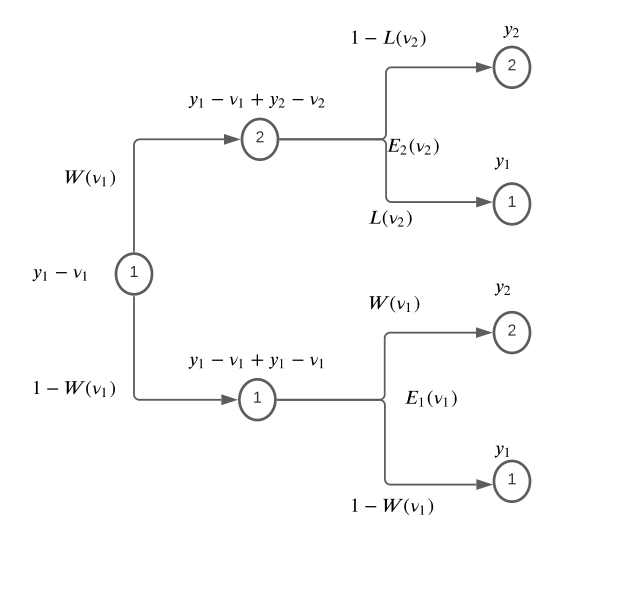
\includegraphics[width=3.5in]{subchapters/two_stage_band1}
\par\end{centering}
\caption{Two period choice for consumer 1\label{fig:Two-period-choice-consumer1}}
\end{figure}

\begin{figure}[t]
\begin{centering}
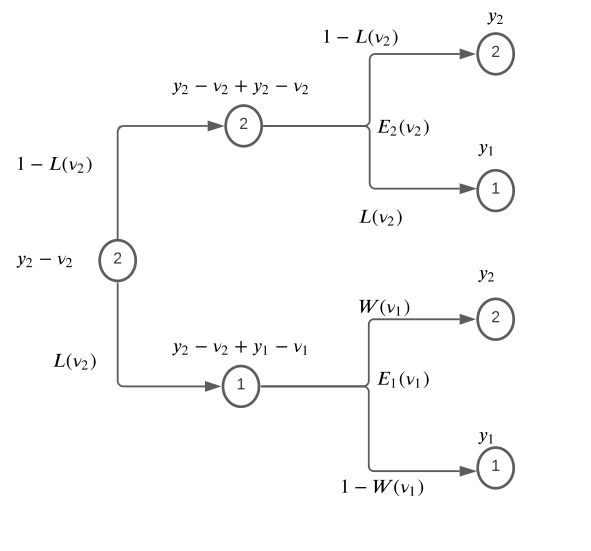
\includegraphics[width=3.5in]{subchapters/two_stage_band2}
\par\end{centering}
\caption{Two period choice for consumer 2 \label{fig:Two-period-choice-consumer2}}
\end{figure}

Assuming that the consumers consider only the assets before removing
$\bar{\nu}_{1}$ or $\bar{\nu}_{2}$ from $y_{1}$ or $y_{2}$ respectively
after the reset, the long-term equilibrium implies that the consumer
1 and 2 have the same expected asset value from being in band 1 or
band 2 after the reset. In other words, the consumer 1 and consumer
2 would replicate each other's behaviour when they swap places with
each other in the status game. Thus at $t=1$, the consumer in band
1 would maximise the utility from the total assets over the two periods

\begin{multline}
u_{1}(\bar{\nu}_{1},\bar{\nu}_{2})\equiv W(\bar{\nu}_{1})u(y_{1}-\bar{\nu}_{1}+y_{2}-\bar{\nu}_{2}+E_{2}(\bar{\nu}_{2}))+(1-W(\bar{\nu}_{1}))u(y_{1}-\bar{\nu}_{1}+y_{1}-\bar{\nu}_{1}+E_{1}(\bar{\nu}_{1}))\label{eq:consumer1_two_stage_util}
\end{multline}

On the other hand, the consumer in band 2 would maximise the following
expected utility from total assets over the two periods

\begin{multline}
u_{2}(\bar{\nu}_{1},\bar{\nu}_{2})=L(\bar{\nu}_{2})u(y_{2}-\bar{\nu}_{2}+y_{1}-\bar{\nu}_{1}+E_{1}(\bar{\nu}_{1}))+(1-L(\bar{\nu}_{2}))u(y_{2}-\bar{\nu}_{2}+y_{2}-\bar{\nu}_{2}+E_{2}(\bar{\nu}_{2}))\label{eq:consumer2_two_stage_util}
\end{multline}

The key difference from the finite-horizon short-term equilibrium
is that the expected utilities depend both on $\bar{\nu}_{1}$, $\bar{\nu}_{2}$
for the consumers. As they choose $\bar{\nu}_{1}$, $\bar{\nu}_{2}$
only once, a high $\bar{\nu}_{1}$ , $\bar{\nu}_{2}$ means hope for
a favourable transition while choosing a low $\bar{\nu}_{1}$ , $\bar{\nu}_{2}$
means relying on accumulation. While the above could be generalised
for a general $T$, we continue to look at the implications for the
optimal choice in the long-term in more detail with the above two-period
set up.

The above long-term conditions imply that a higher $\bar{\nu}_{1}$
makes the loss to a lower band more acceptable for the consumer in
band 2. A peer effect kicks in some sense - due to the fact that the
richer consumer absorbs (replicates) the choice made by poorer consumers
as she is demoted to band 1 and thus the choice of the poorer band
is also factored into her choice in the starting period. Similarly,
a higher $\bar{\nu}_{2}$ might make staying in the poorer band more
appealing for the consumer 1.

If the total assets acquired by the consumer may be considered the
only notion of welfare in the economy, the above model also allows
us to evaluate if the consumers are better off in the long-term with
assets they accumulate with the choice of long-term $\bar{\nu}_{1}$
and $\bar{\nu}_{2}$. More specifically, if $\bar{\nu}_{1}$,$\bar{\nu}_{2}$
are selected by maximising a certain utility, the expected assets
over the two periods for consumer 1 and 2 are simply

\begin{align*}
E(A_{1})= & W(\bar{\nu}_{1})(y_{1}-\bar{\nu}_{1}+y_{2}-\bar{\nu}_{2}+E_{2}(\bar{\nu}_{2}))+(1-W(\bar{\nu}_{1}))(y_{1}-\bar{\nu}_{1}+y_{1}-\bar{\nu}_{1}+E_{1}(\bar{\nu}_{1}))
\end{align*}

\begin{align*}
E(A_{2})= & L(\bar{\nu}_{2})(y_{2}-\bar{\nu}_{2}+y_{1}-\bar{\nu}_{1}+E_{1}(\bar{\nu}_{1}))+(1-L(\bar{\nu}_{2}))(y_{2}-\bar{\nu}_{2}+y_{2}-\bar{\nu}_{2}+E_{2}(\bar{\nu}_{2}))
\end{align*}

To recap, since $A_{T}$ is always bounded for any general $T(\ge2)$,
a maximal $\bar{\nu}_{1}$ or $\bar{\nu}_{2}$ can always be selected
(by consumers 1 and 2 respectively).

\subsubsection{Population stability condition}

\noindent

The condition of population stability (see Equation \ref{eq:population_stability})
constraints the selection of $\bar{\nu}_{1}$ and $\bar{\nu}_{2}$
that is allowed in the short-term. More specifically, the conditions
implies the following in a two-band economy,

\begin{gather*}
W_{1}(\bar{\nu}_{1})=L_{2}(\bar{\nu}_{2})
\end{gather*}

The above relation between the selection $\bar{\nu}_{1}$ and $\bar{\nu}_{2}$
made by the consumer in the long-term (for the two-band economy) helps
us define the functions $\phi(\cdot),\psi(\cdot)$ so that $\bar{\nu}_{1}=\psi(\bar{\nu}_{2})=W^{-1}(L(\bar{\nu}_{2}))$
and $\bar{\nu}_{2}=\phi(\bar{\nu}_{1})=L^{-1}(W(\bar{\nu}_{1}))$.
This also means that the utilities $u_{1}$ and $u_{2}$ maximised
by the consumer can be written in term of either $\bar{\nu}_{1}$
or $\bar{\nu}_{2}$. This is akin to the consumer 1 ( or consumer
2 ) optimising her utility $u_{1}$ (or $u_{2}$) subject to the constraint
$\bar{\nu}_{2}=\phi(\bar{\nu}_{1})$.

\begin{gather*}
u_{1}\equiv u_{1}(\bar{\nu}_{1},\bar{\nu}_{2})=W(\bar{\nu}_{1})u(y_{1}-\bar{\nu}_{1}+y_{2}-\bar{\nu}_{2}+E_{2}(\bar{\nu}_{2}))\\
+(1-W(\bar{\nu}_{1}))u(y_{1}-\bar{\nu}_{1}+y_{1}-\bar{\nu}_{1}+E_{1}(\bar{\nu}_{1}))\\
\Rightarrow u_{1}=W(\bar{\nu}_{1})u(y_{1}-\bar{\nu}_{1}+y_{2}-\phi(\bar{\nu}_{1})+W(\bar{\nu}_{1})y_{1}+(1-W(\bar{\nu}_{1}))y_{2})\\
+(1-W(\bar{\nu}_{1}))u(y_{1}-\bar{\nu}_{1}+y_{1}-\bar{\nu}_{1}+W(\bar{\nu}_{1})y_{2}+(1-W(\bar{\nu}_{1}))y_{1})
\end{gather*}

With $\bar{\nu}_{1}=\psi(\bar{\nu}_{2})$ , the consumer 2 solves
the equivalent problem,

\begin{gather*}
u_{2}\equiv u_{2}(\bar{\nu}_{1},\bar{\nu}_{2})=L(\bar{\nu}_{2})u(y_{2}-\bar{\nu}_{2}+y_{1}-\bar{\nu}_{1}+E_{1}(\bar{\nu}_{1}))\\
+(1-L(\bar{\nu}_{2}))u(y_{2}-\bar{\nu}_{2}+y_{2}-\bar{\nu}_{2}+E_{2}(\bar{\nu}_{2}))\\
\Rightarrow u_{2}=L(\bar{\nu}_{2})u(y_{2}-\bar{\nu}_{2}+y_{1}-\psi(\bar{\nu}_{2})+(1-L(\bar{\nu}_{2}))y_{1}+L(\bar{\nu}_{2})y_{2})\\
+(1-L(\bar{\nu}_{2}))u(y_{2}-\bar{\nu}_{2}+y_{2}-\bar{\nu}_{2}+(1-L(\bar{\nu}_{2}))y_{2}+L(\bar{\nu}_{2})y_{1})
\end{gather*}

Notice that as long as $\phi(\nu)$ and $\psi(\nu)$ are differentiable,
the population condition ensures that $\frac{\partial u_{2}}{\partial\bar{\nu}_{1}}=\frac{\partial u_{2}}{\partial\bar{\nu}_{2}}=0$
($\because\frac{\partial u_{2}}{\partial\bar{\nu}_{2}}=0\Rightarrow\frac{\partial u_{2}}{\partial\bar{\nu}_{1}}=\frac{\partial u_{2}}{\partial\bar{\nu}_{2}}\frac{\partial\phi}{\partial\bar{\nu}_{1}}=0$).
For consumer 1, the first-order condition is 

\begin{gather*}
\frac{\partial u_{1}}{\partial\bar{\nu}_{1}}=\frac{\partial F_{1}}{\partial\bar{\nu}_{1}}+\frac{\text{\ensuremath{\partial F_{2}}}}{\partial\bar{\nu}_{1}}=0
\end{gather*}

where 
\begin{gather*}
F_{1}=W(\bar{\nu}_{1})u(y_{1}-\bar{\nu}_{1}+y_{2}-\phi(\bar{\nu}_{1})+W(\bar{\nu}_{1})y_{1}+(1-W(\bar{\nu}_{1}))y_{2})\\
F_{2}=(1-W(\bar{\nu}_{1}))u(2y_{1}-2\bar{\nu}_{1}+W(\bar{\nu}_{1})y_{2}+(1-W(\bar{\nu}_{1}))y_{1})
\end{gather*}

\begin{multline*}
\frac{\partial F_{1}}{\partial\bar{\nu}_{1}}=W'(\bar{\nu}_{1})u(y_{1}-\bar{\nu}_{1}+y_{2}-\phi(\bar{\nu}_{1})+W(\bar{\nu}_{1})y_{1}+(1-W(\bar{\nu}_{1}))y_{2})-W(\bar{\nu}_{1})(1+\phi'(\bar{\nu}_{1})+W'(\bar{\nu}_{1})y_{2}\\
-W'(\bar{\nu}_{1})y_{1})u'(y_{1}-\bar{\nu}_{1}+y_{2}-\phi(\bar{\nu}_{1})+W(\bar{\nu}_{1})y_{1}+(1-W(\bar{\nu}_{1}))y_{2})
\end{multline*}

\begin{multline*}
\frac{\text{\ensuremath{\partial F_{2}}}}{\partial\bar{\nu}_{1}}=(-W'(\bar{\nu}_{1}))u(2y_{1}-2\bar{\nu}_{1}+W(\bar{\nu}_{1})y_{2}+(1-W(\bar{\nu}_{1}))y_{1})\\
+(1-W(\bar{\nu}_{1}))(-2+y_{2}W'(\bar{\nu}_{1})-y_{1}W'(\bar{\nu}_{1}))u'(2y_{1}-2\bar{\nu}_{1}+W(\bar{\nu}_{1})y_{2}+(1-W(\bar{\nu}_{1}))y_{1})
\end{multline*}

While it is possible to proceed with the techniques used in Section
\ref{subsec:short-term-equilibrium} using a particular form of $\phi(.)$,
we focus on specific forms of $W(\nu),L(\nu)$ for our further discussion.
Instead of suggesting a functional form of $\phi(\nu)$ (or equivalently
$\psi(\nu)$), we explore the characteristics of status competitions
implied by the properties of particular forms of $W(\nu)$ and $L(\nu)$.
These particular forms - along the utility $u(\Lambda)=\Gamma\times\Lambda^{\alpha}$
($\Gamma$, $\alpha$ being constants while $\Lambda$ is the asset
accumulated) that we have used before - are used in essence to examine
the risks shared between the bands as the income difference increases
or decreases in a long-term equilibrium. 

% Discontinuity: Before reset the the consumer accumulates and after the reset her asset disappears. The combined utility is maximised the final expected assets and the consumer cannot maximise at t=1 without considering what happens after (e.g. another consumer comes, L,W change etc.). Further, since the choice at t=1 is different from choice at t=0 if considering the next period alone, a single nu for two time periods can only be forced.  The total assets which we consider are different in the current assets where the decision is being made. The same asset can be enjoyed more in the poorer band and that matters only when utilities are considered i.e. after summing them up over time.
% Discarding intertemporal substitution - The solution with intertemporal utility has the advantage that it provides a control for whether consumers care more about the long-term transition or the the accumulation. Long-term movements are not influenced by savings at all (all savings are meant to go to waste in the long run). This also allows us to "approximate" the case with general  with a discount-factor. The intertemporal methods does however go against the central argument that consumers maximise long-term accumulations. We are left with no options but to rely on the same nu for both periods in order to explain the substitution between later and earlier risk.

\subsection{\label{subsec:Equilibria-particular}Particular mobility functions }

\noindent

The selection of $W(\nu)$ and $L(\nu)$ rests upon two properties
that we have briefly discussed. First, the status competitions can
never guarantee a reward to the next band i.e.$\nexists\nu$ such
that $W(\nu)=1$. Second, that any consumer with a higher $\nu$ should
be rewarded with a higher probability than a consumer with a lower
$\nu$ i.e. $\forall\nu_{1}>\nu_{2}$ we have $W(\nu_{1})>W(\nu_{2})$
and equivalently $L(\nu_{1})<L(\nu_{2})$ with $\forall\nu_{1}>\nu_{2}$.

With these specifications, we assume a logistic form for $W(\nu_{1})$
as a general formulation 

\begin{align}
W(\nu) & =\frac{1}{1+e^{-\omega(\nu-\text{\ensuremath{\underbar{\ensuremath{\omega}}}})}}\label{eq:particular_W_nu_definition}
\end{align}

%lambda = .1 ; bar_lambda = 50; x<-seq(0,100,.1); plot(x,1/(1+exp(-lambda * (x-bar_lambda))),type='l',xlab=latex2exp::TeX("$\\nu$"),ylab=latex2exp::TeX("$W(\\nu)$"),lty=1); lines(x,1/(1+exp(-lambda*2 * (x-bar_lambda))),type='l',lty=2); lines(x,1/(1+exp(-lambda*.5 * (x-bar_lambda))),type='l',lty=3); legend(60, .4, legend=c(latex2exp::TeX("$ \\omega = 0.1$"),latex2exp::TeX("$ \\omega = 0.2$"),latex2exp::TeX("$ \\omega = 0.05$")) , lty=c(1,2,3), cex=0.7)

The above specification only considers $W(\nu)$ where $\frac{\partial W}{\partial\nu}$
is symmetrical around $\underline{\omega}$ i.e. the probability to
rise to the next band rises and drops at the same rate around $\underline{\omega}$.
The same applies to the equivalent definition for $L(\nu)$. When
considering the population stability in band, the above specification
translates into a simple linear relationship between the parameters
that we discuss below. While a $\frac{\partial W}{\partial\nu}$ that
is asymmetrical around $\underline{\omega}$ may provide a more general
specification of $W(\nu)$ and $L(\nu)$, the results that we derive
from the specification are independent of whether $\frac{\partial W}{\partial\nu}$
is symmetrical around $\underline{\omega}$ around or not.

There are certain implications of the parameters for the nature of
status competitions. First, the parameter $\omega$ determines how
sharp the probability of promotion $W(\nu)$ would rise with $\nu$.
The plots of $W(\nu)$ defined in Equation \ref{eq:particular_W_nu_definition}
are shown in Figure \ref{fig:W_nu_parameters}. The parameter $\underbar{\ensuremath{\omega}}$,
on the other hand, represents whether a significant rise in probability
occurs for a high $\nu$ (corresponding to a high $\text{\ensuremath{\underbar{\ensuremath{\omega}}}}$)
or relatively low $\nu$ (corresponding to a low $\text{\ensuremath{\underbar{\ensuremath{\omega}}}}$).
Roughly speaking, with $W(\nu)$ being the upward mobility in the
two-consumer economy, $\omega$ is the degree of separation in bands
imposed by the spending on $\nu$. A high $\omega$ differentiates
the outcome of those having low $\nu$ from those having higher $\nu$
more clearly. The parameter $\text{\ensuremath{\underbar{\ensuremath{\omega}}}}$-
on the other hand - is the minimum $\nu$ for there to be a probability
of transition to the next income band. It thus represents the level
of $\nu$ at which status competitions become significant in the economy.
We focus on the $\underbar{\ensuremath{\omega}}$ implied by long-term
equilibria - since a high $\underbar{\ensuremath{\omega}}$ means
a higher $\nu$ required for mobility and a low $\underbar{\ensuremath{\omega}}$
means low mobility. The plots for varying $\underbar{\ensuremath{\omega}}$
are shown in Figure \ref{fig:W_nu_parameters_means}.

%lambda = .1 ; bar_lambda = 50; x<-seq(0,100,.1); plot(x,1/(1+exp(-lambda * (x-bar_lambda))),type='l',xlab=latex2exp::TeX("$\\nu$"),ylab=latex2exp::TeX("$W(\\nu)$"),lty=1); lines(x,1/(1+exp(-lambda*(x-bar_lambda-20))),type='l',lty=2); lines(x,1/(1+exp(-lambda*(x-bar_lambda+20))),type='l',lty=3) ; legend(60, .4, legend=latex2exp::TeX(paste("$ \\bar{\\omega}=",c(50,70,30),"$")) , lty=c(1,2,3), cex=0.7)

\begin{figure}[H]
\begin{centering}
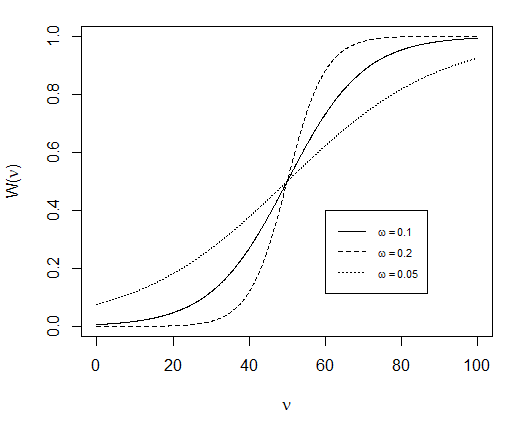
\includegraphics[width=3.5in]{subchapters/plots_logistic_function}
\par\end{centering}
\caption{\label{fig:W_nu_parameters}$W(\nu)$ parameter $\omega$}
\end{figure}

\begin{figure}[H]
\begin{centering}
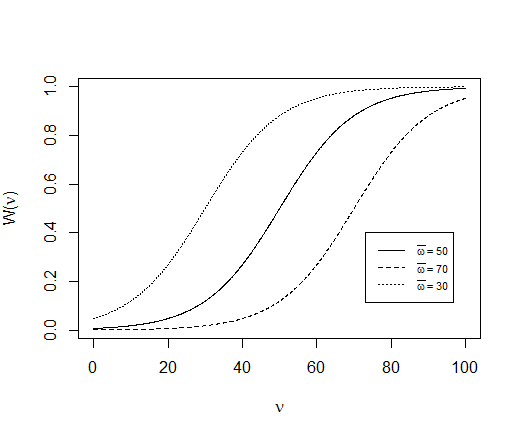
\includegraphics[width=3.5in]{subchapters/plots_logistic_function_means}
\par\end{centering}
\caption{\label{fig:W_nu_parameters_means}$W(\nu)$ parameter $\underline{\omega}$ }
\end{figure}

Just as $W(\nu)$ represents the upward mobility, $1-L(\nu)$ represents
the security associated with the higher income band. The form of $L(\nu_{2})$
with parameters $\lambda$, $\underbar{\ensuremath{\lambda}}$ is
as follows

\begin{align}
L(\nu) & =1-\frac{1}{1+e^{-\lambda(\nu-\underbar{\ensuremath{\lambda}})}}\label{eq:L_nu_definition}
\end{align}

Similar to the parameters $\omega$ and $\underline{\omega}$, the
parameter $\lambda$ separates winners and losers through $L(\nu)$
(see plots in Figure \ref{fig:L_loss_parameters} ) and the level
of $\nu$ where competitions become significant is driven by the parameter
$\underbar{\ensuremath{\lambda}}$ (see Plots in Figure \ref{fig:L_loss_parameters_mean}).
We use the constraints on this parameter to explain how status investments
may rise or fall for a fixed set of $\lambda$ and $\omega$.

\begin{figure}[H]
\begin{centering}
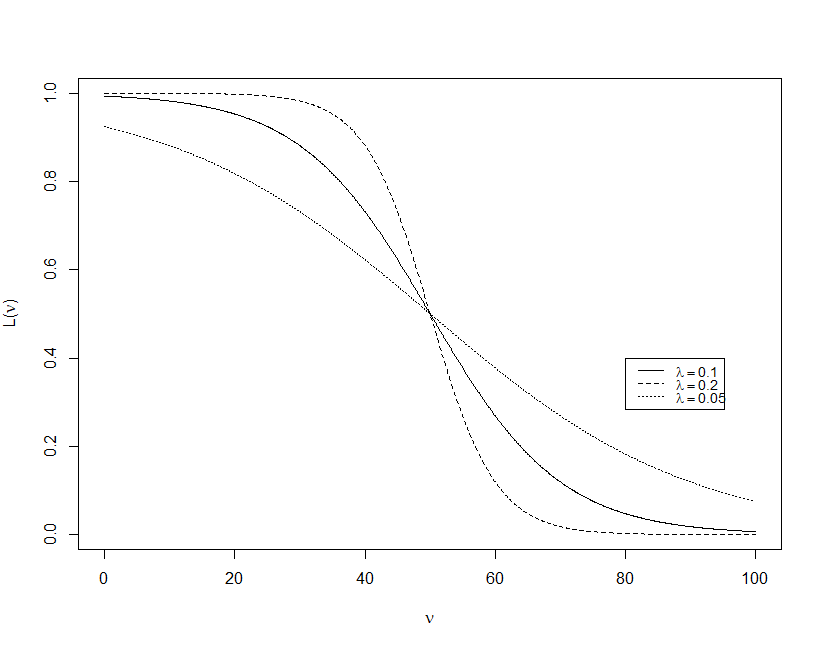
\includegraphics[width=3.5in]{subchapters/plots_logistic_function_l}
\par\end{centering}
\caption{\label{fig:L_loss_parameters}$L(\nu)$ parameter $\lambda$}
\end{figure}

\begin{figure}[H]
\begin{centering}
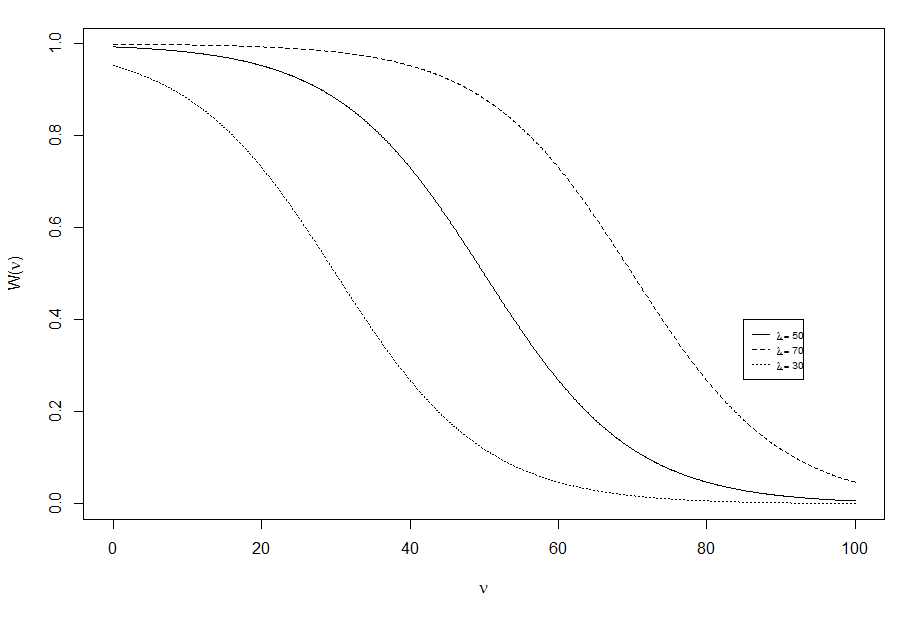
\includegraphics[width=3.5in]{subchapters/plots_logistic_function_l_means}
\par\end{centering}
\caption{\label{fig:L_loss_parameters_mean}$L(\nu)$ parameter $\underline{\lambda}$}
\end{figure}

% LAMBDA_BAR PLOT : lambda = .1 ; bar_lambda = 50; x<-seq(0,100,.1); plot(x,1-1/(1+exp(-lambda * (x-bar_lambda))),type='l',xlab=latex2exp::TeX("$\\nu$"),ylab=latex2exp::TeX("$W(\\nu)$"),lty=1); lines(x,1-1/(1+exp(-lambda*(x-bar_lambda-20))),type='l',lty=2); lines(x,1-1/(1+exp(-lambda*(x-bar_lambda+20))),type='l',lty=3) ; legend(85, .4, legend=latex2exp::TeX(paste("$ \\underline{\\lambda}=",c(50,70,30),"$")) , lty=c(1,2,3), cex=0.6)

% [fixing \omega, \lambda] When income differences are low, the consumers would spend more on status consumption - because there is some difference in asset still. But we expect competition to narrow - that could mean either or both of i) a sharp response to \nu i.e. high \omega or ii) a higher \bar{\omega} so that there are no gains until a certain level is reached. Again magnitude of \omega does not seem to matter in our story - as it only seems to suggest a discreteness in competition i.e. whether the consumer below a certain threshold get no benefit at all. We do however see curvature effect on \omega - so setting \kappa\ne1 seems one way to get a curvature to the poorer consumer - increasing lambda_bar also adds curvature to consumer 1 i.e. requiring a high \nu_{2} for security incentivises the consumer 1 as well

Notice that the optimisation of utility with the other consumer's
choice fixed (i.e. optimisation of utility by choosing$\bar{\nu}_{1}$
for consumer 1 when $\bar{\nu}_{2}'$ is fixed or the optimisation
of utility by choosing$\bar{\nu}_{2}$ by consumer 2 when $\bar{\nu}_{1}'$
is fixed ) is not very different from the the optimisation in short-term.
Given the particular forms of $W(\nu)$ and $L(\nu)$ in Equations
\ref{eq:particular_W_nu_definition} and \ref{eq:L_nu_definition}
and a utility function $u(\Lambda)$ for assets $\Lambda$ (in a particular
time period), the Equations \ref{eq:consumer1_two_stage_util} and
\ref{eq:consumer2_two_stage_util} can be rewritten so that the consumer
1 chooses a $\bar{\nu}_{1}$ to maximise the following utility for
a $\bar{\nu}_{2}'$ chosen by consumer 2

\begin{gather*}
u_{1}(\bar{\nu}_{1},\bar{\nu}_{2}')=W(\bar{\nu}_{1})u(y_{1}-\bar{\nu}_{1}+y_{2}-\bar{\nu}_{2}'+E_{2}(\bar{\nu}_{2}'))+(1-W(\bar{\nu}_{1}))u(y_{1}-\bar{\nu}_{1}+y_{1}-\bar{\nu}_{1}+E_{1}(\bar{\nu}_{1}))
\end{gather*}

Choosing $u(\Lambda)=\Gamma\cdot\Lambda^{\alpha}$(where $\alpha$
is a constant), the above can be written as

\begin{gather*}
u_{1}(\bar{\nu}_{1},\bar{\nu}_{2}')=\frac{\Gamma(y_{1}+y_{2}-\bar{\nu}_{1}+E_{2}(\bar{\nu}_{2}')-\bar{\nu}_{2}')^{\alpha}}{1+e^{-\omega(\bar{\nu}_{1}-\text{\ensuremath{\underbar{\ensuremath{\omega}}}})}}+\frac{\Gamma(2y_{1}-2\bar{\nu}_{1}+E_{1}(\bar{\nu}_{1}))^{\alpha}}{1+e^{\omega(\bar{\nu}_{1}-\text{\ensuremath{\underbar{\ensuremath{\omega}}}})}}
\end{gather*}

Similarly, the consumer 2 chooses $\bar{\nu}_{2}$ to maximise the
following utility for a given $\bar{\nu}_{1}'$ chosen by consumer
1

\begin{gather*}
u_{2}(\bar{\nu}_{1}',\bar{\nu}_{2})=\frac{\Gamma(y_{2}-\bar{\nu}_{2}+y_{1}-\bar{\nu}_{1}'+E_{1}(\bar{\nu}_{1}'))^{\alpha}}{1+e^{\lambda(\bar{\nu}_{2}-\underbar{\ensuremath{\lambda}})}}+\frac{\Gamma(y_{2}-\bar{\nu}_{2}+y_{2}-\bar{\nu}_{2}+E_{2}(\bar{\nu}_{2}))^{\alpha}}{1+e^{-\lambda(\bar{\nu}_{2}-\underbar{\ensuremath{\lambda}})}}
\end{gather*}

Defining $k_{1}\equiv E_{1}(\bar{\nu}_{1}^{*})-\bar{\nu}_{1}^{*}$
and $k_{2}\equiv E_{2}(\bar{\nu}_{2}^{*})-\bar{\nu}_{2}^{*}$ as the
deviation from the expected of income from band-promotion (or demotion),
we can also write 

\begin{gather*}
u_{1}(\bar{\nu}_{1})=\frac{\Gamma(y_{1}+y_{2}-\bar{\nu}_{1}+k_{2})^{\alpha}}{1+e^{-\omega(\bar{\nu}_{1}-\text{\ensuremath{\underbar{\ensuremath{\omega}}}})}}+\frac{\Gamma(2y_{1}-2\bar{\nu}_{1}+E_{1}(\bar{\nu}_{1}))^{\alpha}}{1+e^{\omega(\bar{\nu}_{1}-\text{\ensuremath{\underbar{\ensuremath{\omega}}}})}}
\end{gather*}

\begin{gather*}
u_{2}(\bar{\nu}_{2})=\frac{\Gamma(y_{1}+y_{2}-\bar{\nu}_{2}+k_{1})^{\alpha}}{1+e^{\lambda(\bar{\nu}_{2}-\underbar{\ensuremath{\lambda}})}}+\frac{\Gamma(2y_{2}-2\bar{\nu}_{2}+E_{2}(\bar{\nu}_{2}))^{\alpha}}{1+e^{-\lambda(\bar{\nu}_{2}-\underbar{\ensuremath{\lambda}})}}
\end{gather*}

The functions $E_{1}(\bar{\nu}_{1})$ and $E_{2}(\bar{\nu}_{2})$
used above are set as follows using the specific forms of $u(\Lambda)$,
$W(\nu)$ and $L(\nu)$ . The selection of $\bar{\nu}_{1}$ by the
consumer 1 based on $\omega$, $\text{\ensuremath{\underbar{\ensuremath{\omega}}}}$
is evidently symmetric to the selection of $\bar{\nu}_{2}$ based
on $\lambda$, $\text{\ensuremath{\underbar{\ensuremath{\lambda}}}}$
by the consumer 2.

\begin{gather*}
E_{1}(\bar{\nu}_{1})=W(\bar{\nu}_{1})y_{2}+(1-W(\bar{\nu}_{1}))y_{1}\\
=\frac{y_{2}}{1+e^{-\omega(\bar{\nu}_{1}-\text{\ensuremath{\underbar{\ensuremath{\omega}}}})}}+\frac{y_{1}}{1+e^{\omega(\bar{\nu}_{1}-\text{\ensuremath{\underbar{\ensuremath{\omega}}}})}}
\end{gather*}

\begin{gather*}
E_{2}(\bar{\nu}_{2})=(1-L(\bar{\nu}_{2}))y_{2}+L(\bar{\nu}_{2})y_{1}\\
=\frac{y_{2}}{1+e^{-\lambda(\bar{\nu}_{2}-\underbar{\ensuremath{\lambda}})}}+\frac{y_{1}}{1+e^{\lambda(\bar{\nu}_{2}-\underbar{\ensuremath{\lambda}})}}
\end{gather*}

While an explicit solution of the first-order conditions for the above
may be less trivial, it is easy to show numerically that higher income
differences $y_{2}-y_{1}$ increase both $\bar{\nu}_{1}$ and $\bar{\nu}_{2}$
. Also, an increase in $k_{1}$ ( i.e. less $E_{1}(\bar{\nu}_{1}^{*})-\bar{\nu}_{1}^{*}$)
decreases $\bar{\nu}_{2}$ while increasing $k_{2}$ ( i.e. less $E_{2}(\bar{\nu}_{2}^{*})-\bar{\nu}_{2}^{*}$
) decreases $\bar{\nu}_{1}$. 

As we now show, the increases in $\bar{\nu}_{1}$ and $\bar{\nu}_{2}$
are balanced by long-term consequences of population stability conditions.
Such a long-term solution which accommodates the population stability
can be assumed to imply a planner that directs the various selections
$\{\bar{\nu}_{1},\bar{\nu}_{2}\}$ implied by the above optimisation
of above utilities. In other words, a combined utility $\mathscr{U}$
for both the consumers can be assumed to be maximised while the population
stability conditions are implied. To explore a detailed numerical
solution of the equilibrium, we therefore focus on a cooperative solution
using a combined utility $\mathscr{U}$ for both the consumers.

The cooperative approach that we explain the effect of income differences
$\Delta=y_{2}-y_{1}$ with imposes two constraints on the set of parameters
$\omega$, $\text{\ensuremath{\underbar{\ensuremath{\omega}}}}$,
$\lambda$, $\text{\ensuremath{\underbar{\ensuremath{\lambda}}}}$.
First is the population stability condition with the specific forms
of $W(\nu)$ and $L(\nu)$. More specifically, the population constraint
$W(\nu_{1}^{*})=L(\nu_{2}^{*})$ implies a relationship between $\text{\ensuremath{\bar{\nu}_{1}}}$
and $\bar{\nu}_{2}$ as follows\footnote{$\frac{1}{1+e^{-\omega(\nu-\underbar{\ensuremath{\omega}})}}+\frac{1}{1+e^{-\lambda(\nu-\underbar{\ensuremath{\lambda}})}}=1$
$\Rightarrow$$(1+e^{-\omega(\nu-\underbar{\ensuremath{\omega}})})(1+e^{-\lambda(\nu-\underbar{\ensuremath{\lambda}})})=1+e^{-\omega(\nu-\underbar{\ensuremath{\omega}})}+1+e^{-\lambda(\nu-\underbar{\ensuremath{\lambda}})}$} 

\begin{align}
\omega(\bar{\nu}_{1}-\underbar{\ensuremath{\omega}})+\lambda(\bar{\nu}_{2}-\underbar{\ensuremath{\lambda}}) & =0\label{eq:param_constraint}
\end{align}

The second constraint is through a combined utility for the rich and
poor consumers in the economy that we detail in Section \ref{subsec:CombinedUtilOptimisation}.
Since we have limited our attention to the growing economies where
status competitions determine promotion more sharply than demotion,
we focus only on cases where $\omega>\lambda$ ($\kappa>1$ ) and
assume that $\omega$ as well as $\lambda$ are fixed for the rest
of our discussion. With fixed $\omega$ and $\lambda$, the cooperative
solution with the population stability constraint and the maximal
combined utility is used to eliminate $\text{\ensuremath{\underbar{\ensuremath{\omega}}}}$
and $\text{\ensuremath{\underbar{\ensuremath{\lambda}}}}$. Before
we detail this cooperative equilibrium, consider however the relationship
between $\bar{\nu}_{1}$ and $\bar{\nu}_{2}$ which the population
stability alone indicates.

% \kappa does not mean segregation. Rather, it means how asymmetric rise vs fall is. The magnitude of \lambda and \omega themselves do not mean segregation either - they only mean forcing a certain level of \nu. For our purposes, we might just fix \omega,\lambda. What we need to worry about is the changes in economy do not change \omega, \lambda. The argument might go that as equality approaches consumers would spend more on status consumption as they have less avenues to rise above the others. If so, \omega would get flattened. We don't have a model of how income differences cause this. What we have endogenised is only how differences income respond to intrinsic greed. \omega, \bar{\omega},\lambda,\bar{\lambda} relationship has not been cleared. The segregation is in fact meant by \nu_{1}=0 (\nu_{2}=0 and \nu_{1}>0 does not mean no status consumption).

Setting $\kappa\equiv\frac{\omega}{\lambda}$ , we have $(\bar{\nu}_{1}-\underbar{\ensuremath{\omega}})=-\kappa(\bar{\nu}_{2}-\underbar{\ensuremath{\lambda}})$
so that consumers must balance $\bar{\nu}_{1}$ and $\bar{\nu}_{2}$
on either side of $\text{\ensuremath{\underbar{\ensuremath{\omega}}}}$
and $\underbar{\ensuremath{\lambda}}$. Another way to interpret $\nu_{1}^{*}=\underbar{\ensuremath{\omega}}-\kappa(\nu_{2}^{*}-\underbar{\ensuremath{\lambda}})$
is that the poorer consumer's long-term expenditure towards status
rises with the level at which upward transition becomes significant
and falls with richer consumer's excessive spending. It is worth noting
that the population stability condition is independent of any consumer
utilities that the consumers use to make choices for $\bar{\nu}_{1}$
and $\bar{\nu}_{2}$ or whether one views the cooperative or Nash
equilibrium as solutions. 

The level at which upward transition becomes significant raises poor
consumer's expenditure towards status is less surprising. What's more
interesting is the withdrawal of the poorer consumer from the status
competition due to a higher status investment  by the richer consumer.
The population constraint - under the assumption $\kappa>1$ - readily
provides the condition of withdrawal from status competitions for
either of the consumers in the economy. More particularly, there would
be no benefits to the consumer from expenditure towards status when
either $\overline{\nu}_{1}\rightarrow0$ or $\overline{\nu}_{2}\rightarrow0$
is implied in the long-term. Since $\overline{\nu}_{1}$ and $\overline{\nu}_{2}$
are known in terms of $\text{\ensuremath{\underbar{\ensuremath{\lambda}}}}$,$\text{\ensuremath{\underbar{\ensuremath{\omega}}}}$
($\omega$,$\lambda$ are already known and fixed) for given utilities,
the condition $\frac{\underbar{\ensuremath{\omega}}}{\kappa}+\overline{\lambda}=\overline{\nu}_{2}$
as $\overline{\nu}_{1}\rightarrow0$ sets the $\underline{\omega}$
for a given level of security $\underline{\lambda}$ that must exist
for there to be a status competition with non-zero $\bar{\nu}_{2}$.
In other words, for consumer 1 to participate in the status competition,
the consumer 2 must choose $\overline{\nu}_{2}<\frac{\underbar{\ensuremath{\omega}}}{\kappa}+\text{\ensuremath{\underbar{\ensuremath{\lambda}}}}$
. Similarly, $\bar{\nu}_{2}>0$ implies $\bar{\nu}_{1}$$<$$\kappa\underline{\lambda}+\underline{\omega}$
i.e. if the consumer 1 spends more than $\kappa\underline{\lambda}+\underline{\omega}$,
the likelihood of her getting into the richer band is so high relative
to the security offered to the consumer 2 through status competition
that there would be no reason for any expenditure towards status for
the richer consumer. Notice that these constraints indeed uphold for
any utility maximised by the consumer. To explore the effect of income
differences $\Delta=y_{2}-y_{1}$ on the selection of $\bar{\nu}_{1}$
and $\bar{\nu}_{2}$ by the poor and rich consumers, we now explore
a cooperative solution numerically for a given $\kappa$ where both
the population stability condition and a combined utility for the
two consumers are considered.

\subsubsection{\label{subsec:CombinedUtilOptimisation}Optimal utility for fixed
$\ensuremath{\omega}$ and $\lambda$}

\noindent

With fixed values of $\omega$ and $\lambda$, the condition other
than the population stability (see Equation \ref{eq:param_constraint}.)
that helps determine the remaining parameters $\underline{\omega}$
and $\underline{\lambda}$ is arrived at by viewing the selection
of $\bar{\nu}_{1},\bar{\nu}_{2}$ as a multi-objective optimisation
so that an optimal pair $\{\bar{\nu}_{1},\bar{\nu}_{2}\}$ is selected
for the society comprising of two bands. In other words, the values
for $\underline{\omega}$ and $\underline{\lambda}$ are implied by
the population stability condition and the criterion for maximal consumer
utilities - as the parameters $\underline{\omega}$ and $\underline{\lambda}$
( defined as the level of expenditure towards status at which promotion
or demotion in the bands is of material significance ) are eliminated
after fixing $\omega$ and $\lambda$.

Without a loss of generality, $\underline{\lambda}$ is eliminated
with the population stability condition in order for us to explain
the sensitivity of status investments with respect to income difference
$\Delta=y_{2}-y_{1}$. $\underline{\omega}$ then corresponds to the
maximal combined utility for the two consumers. This combined utility
for the two consumers can be viewed as the Pareto-goal for the society
comprising of rich and the poor consumers. A parameter $\beta$ is
used in this combined utility to controls for whether the Pareto goal
relies more on the richer consumer than the poorer consumer. The parameter
$\beta$ could indicate how labour-intensive an economy may be or
how segregated (in terms of the population) the rich and the poor
are in the economy. For the purposes of our discussion, it suffices
that a given long-term income difference $\Delta=y_{2}-y_{1}$ corresponds
to a particular $\underline{\omega}$ when a particular structure
of the combined utility is known. Defining a general form of the combined
(concave) utility - which is maximised collectively for the two consumer
in the two bands - with parameter $\beta$ that tilts society's combined
utility in favour of the richer or poorer consumer, we have

\begin{align}
\mathscr{U} & =f(\beta,\bar{\nu}_{1}^{*},\bar{\nu}_{2}^{*})\label{eq:combined_utility}
\end{align}

Recall that the population stability condition $W(\bar{\nu}_{1})=L(\bar{\nu}_{2})$
provides the following relationship among $\lambda,\underline{\lambda},\omega$
and $\underline{\omega}$ 

\begin{align*}
\omega(\bar{\nu}_{1}-\underbar{\ensuremath{\omega}})+\lambda(\bar{\nu}_{2}-\underbar{\ensuremath{\lambda}}) & =0
\end{align*}

As we have defined $\bar{\nu}_{2}=\phi(\bar{\nu}_{1})$ and $\bar{\nu}_{1}=\psi(\bar{\nu}_{2})$,
we use above to write,

\begin{gather*}
\psi(\bar{\nu}_{2})=\underbar{\ensuremath{\omega}}-(\lambda/\omega)\bar{\nu}_{2}+(\lambda/\omega)\underbar{\ensuremath{\lambda}}\\
\phi(\bar{\nu}_{1})=\underbar{\ensuremath{\lambda}}-(\omega/\lambda)\bar{\nu}_{1}+(\omega/\lambda)\underbar{\ensuremath{\omega}}
\end{gather*}

The above definitions also imply that the utilities for the consumers
can be written either in terms of $\bar{\nu_{1}}$ or $\bar{\nu_{2}}$.
More particularly, if the selection for consumer 1 is represented
with the function $G(\lambda,\underline{\lambda},\text{\ensuremath{\omega},\ensuremath{\underline{\omega}}},y_{1},\Delta)$,
then

\begin{gather}
\bar{\nu}_{1}^{*}=G(\lambda,\underline{\lambda},\text{\ensuremath{\omega},\ensuremath{\underline{\omega}}},y_{1},\Delta)\label{eq:nu1_function}\\
\bar{\nu}_{2}^{*}=\phi(\bar{\nu}_{1}^{*})\nonumber 
\end{gather}

The utility $\mathscr{U}$ is thus a function of $y_{1},\Delta=y_{2}-y_{1}$
and the parameters $\lambda,\underline{\lambda},\text{\ensuremath{\omega},\ensuremath{\underline{\omega}}}$ 

\begin{gather*}
\mathscr{U}=f(\beta,G(\lambda,\underline{\lambda},\text{\ensuremath{\omega},\ensuremath{\underline{\omega}}},y_{1},\Delta),\phi(G(\lambda,\underline{\lambda},\text{\ensuremath{\omega},\ensuremath{\underline{\omega}}},y_{1},\Delta))
\end{gather*}

With a particular form of $\mathscr{U}$ , a $\underline{\omega}$
can be obtained using numerical methods after eliminating $\underline{\lambda}$.
While we pursue this approach in Section \ref{subsec:Numerical-Optimisation},
we consider a solution with the total expenditure on status $\bar{\nu}_{1}^{*}+\bar{\nu}_{2}^{*}$
in the society - a concern that is of interest in its own right. Setting
an upper bound $\xi$ so that $\bar{\nu}_{1}^{*}+\bar{\nu}_{2}^{*}\le\xi$
(i.e. $\xi-\bar{\nu}_{1}^{*}-\bar{\nu}_{2}^{*}\ge0$), the above definition
of $\bar{\nu}_{2}=\phi(\bar{\nu}_{1})$ leads to the following

\begin{gather*}
\frac{\lambda\xi-\omega\underbar{\ensuremath{\omega}}-\underbar{\ensuremath{\lambda}\ensuremath{\lambda}}}{\lambda-\omega}-G(\lambda,\underline{\lambda},\text{\ensuremath{\omega},\ensuremath{\underline{\omega}}},y_{1},y_{2})\ge0
\end{gather*}

The condition $\bar{\nu}_{1}^{*}+\bar{\nu}_{2}^{*}\le\xi$ translates
into the following upper bound for $\bar{\nu}_{1}$. With $\omega>\lambda$
(in a growing economy), it is thus evident that an increase in $\xi$
decreases this bound on $\bar{\nu}_{1}$

\begin{gather*}
\bar{\nu}_{1}=G(\lambda,\underline{\lambda},\text{\ensuremath{\omega},\ensuremath{\underline{\omega}}},y_{1},y_{2})\le\frac{\omega/\lambda\underbar{\ensuremath{\omega}}-(\xi-\underbar{\ensuremath{\lambda}})}{\omega/\lambda-1}
\end{gather*}

Proceeding with first-order conditions under this constraint, the
Lagrangian $L=\mathscr{U}+\mu(\frac{\lambda\xi-\omega\underbar{\ensuremath{\omega}}-\underbar{\ensuremath{\lambda}\ensuremath{\lambda}}}{\lambda-\omega}-G(\lambda,\underline{\lambda},\text{\ensuremath{\omega},\ensuremath{\underline{\omega}}},y_{1},\Delta))$
leads to the following (Kuhn-Tucker) conditions for an interior solution
(notice that all constraints being linear ensures that the following
first-order-conditions is a necessary condition for local-minima -
see \cite{takayamaanalyticalmethods1993} ) where $\mu$ is the Lagrangian
multiplier for the constraint $\bar{\nu}_{1}^{*}+\bar{\nu}_{2}^{*}\le\xi$
.

\begin{align*}
\frac{\partial L}{\partial\underline{\lambda}} & =\frac{\partial L}{\partial\ensuremath{\underline{\omega}}}=0
\end{align*}

and

\begin{align*}
\mu(\frac{\lambda\xi-\omega\underbar{\ensuremath{\omega}}-\underbar{\ensuremath{\lambda}\ensuremath{\lambda}}}{\lambda-\omega}-G(\lambda,\underline{\lambda},\text{\ensuremath{\omega},\ensuremath{\underline{\omega}}},y_{1},y_{2})) & =0
\end{align*}

Two cases therefore arise
\begin{itemize}
\item Case I: $\frac{\lambda\xi-\omega\underbar{\ensuremath{\omega}}-\underbar{\ensuremath{\lambda}\ensuremath{\lambda}}}{\lambda-\omega}=G(\lambda,\underline{\lambda},\text{\ensuremath{\omega},\ensuremath{\underline{\omega}}},y_{1},y_{2})$
i.e. $\bar{\nu}_{1}^{*}+\bar{\nu}_{2}^{*}=\xi$ and $\mu>0$.
\item Case II: $\bar{\nu}_{1}^{*}+\bar{\nu}_{2}^{*}<\xi$ and $\mu=0$ so
that $\frac{\partial\mathscr{U}}{\partial\underline{\lambda}}=0$
corresponds to the unconstrained maximum for $\mathscr{U}$ after
$\bar{\omega}$ is eliminated using the population stability condition
(see below for details).
\end{itemize}
In Case I, the condition $\bar{\nu}_{1}+\bar{\nu}_{2}=\xi$ (with
$\mu\ne0$ ) directly leads to a solution dependent on $\xi$
\begin{gather*}
\bar{\nu}_{1}=G(\lambda,\underline{\lambda},\text{\ensuremath{\omega},\ensuremath{\underline{\omega}}},y_{1},y_{2})=\frac{\lambda\xi-\omega\underbar{\ensuremath{\omega}}-\underbar{\ensuremath{\lambda}\ensuremath{\lambda}}}{\lambda-\omega}
\end{gather*}

or,

\begin{align*}
\frac{\partial G}{\partial\xi} & =\frac{1}{1-\frac{\omega}{\lambda}}
\end{align*}

As long as $\omega>\lambda$, an increase in $\xi$ would decrease
$\bar{\nu}_{1}$ and a decrease in $\xi$ would increase $\bar{\nu}_{1}$.
Finiteness constraints on $\bar{\nu}_{1}^{*}+\bar{\nu}_{2}^{*}$ therefore
suppress the status investments for the poorer consumer. Further,
as long as $\xi$ is an increasing function of $\Delta$ i.e. increasing
income difference between the two consumers always increases the constraint
$\xi$, then $\omega>\lambda$ would mean that an increase in $\Delta$
would decrease $\bar{\nu}_{1}$ and a decrease in $\Delta$ would
increase $\bar{\nu}_{1}$ since 
\begin{gather*}
\frac{\partial G}{\partial\Delta}=\frac{1}{1-\frac{\omega}{\lambda}}\frac{\partial\xi}{\partial\Delta}
\end{gather*}

The results for Case II i.e. of local-maximisation of $u_{1},u_{2}$
when $\xi$ is high enough are less straightforward since both $u_{1},u_{2}$
depend on $\phi(\nu),\psi(\nu)$ - whose specific forms have not been
yet assumed in the solution. Considering a specific form for $u(A)=\Gamma\cdot A^{\alpha}$
and the population stability condition (see Appendix III), the three
unknowns $\underline{\omega},\underline{\lambda}$ and $\bar{\nu}_{1}$
(with fixed $\lambda,\omega$ ) can be solved using the conditions
$\frac{\partial u_{1}}{\partial\bar{\nu}_{1}}=0$ , $\frac{\partial u_{2}}{\partial\bar{\nu}_{1}}=0$
and the optimisation of the combined utility $\mathscr{U}$ (see Equation
\ref{eq:combined_utility}). So long as the form of $\mathscr{U}$
ensures that the $\underline{\lambda}$ can be expressed as a concave
function of $\underline{\omega}$, we can ascertain that a unique
$\underline{\omega}$ would maximise the combined utility $\mathscr{U}$.
Such a solution depends however on the particular form of combined
utility $\mathscr{U}$. The form of a particular $\mathscr{U}$ i.e.
the Pareto concern of how the asset utilities from poor and richer
consumer are combined in a society thus form an important caveat for
the effect of income differences on consumer selections $\bar{\nu}_{1}$
and $\bar{\nu}_{2}$. A simple setting of $\mathscr{U}(u_{1},u_{2})=\beta u_{1}+(1-\beta)u_{2}$
where both consumers are better off with more assets (higher utilities
from assets) - that we explore numerically in Section \ref{subsec:Numerical-Optimisation}
- does not guarantee that the consumers would decrease status investments
with lowering of income differences.

Notice that there are two factors in the cooperative solution with
population stability that balance the increase in $\bar{\nu}_{1}$
and $\bar{\nu}_{2}$ in the long-run. First is that the poorer consumer
eventually runs out of budget $y_{1}$ if the $y_{2}$ is a lot higher
(i.e. when $\Delta=y_{2}-y_{1}$ is very high) and exercises $\bar{\nu}_{1}\rightarrow0$
instead. Second is that the richer consumer withdraws with $\bar{\nu}_{2}\rightarrow0$
if the poorer consumer gets the promotion to a higher band very easily.
Both of these both factors - are a result of the population stability
condition and are thus independent of the combined utility $\mathscr{U}$.
As these factors would continue to hold for a non-cooperative solution,
we can argue that the above dynamics for the effect of $\Delta=y_{2}-y_{1}$
on $\bar{\nu}_{1}$ and $\bar{\nu}_{2}$ in the long-run remain unchanged
for a non-cooperative solution as well.

In summary, the goal of using the two conditions is to explore the
effects of income difference $y_{2}-y_{1}$ on status competitions
while incorporating the changes in competitions that occur to rise
or fall in income-differences in the long-term. With the parameters
controlling a specific form of $W(\nu),L(\nu)$ endogenised within
the equilibrium conditions, we are able to remedy the earlier issue
with the short-term equilibrium that changes in income also change
the competitions and $W(\nu),L(\nu)$ themselves. Unlike with the
short-term equilibrium, in other words, the changes in $\Delta y=y_{2}-y_{1}$
correspond to a different $W(\nu)$, $L(\nu)$ characterised by $\underline{\omega}$
and $\underline{\lambda}$. As we show with numerical methods, this
relationship does not necessarily result in consumers always increasing
$\bar{\nu}_{1}$, $\bar{\nu}_{2}$ in response to rise in income differences.

\subsubsection{\label{subsec:Numerical-Optimisation}A cooperative solution using
Numerical methods}

\noindent

As we explain in Section \ref{subsec:CombinedUtilOptimisation}, the
investments towards future status $\bar{\nu}_{1}$ and $\bar{\nu}_{2}$
correspond to the maximal utility obtained by each consumer (as defined
in Equation \ref{eq:nu1_function} ). With $\lambda$ , $\omega$
fixed for a given set of incomes, $y_{1},y_{2}$, the values of $\text{\ensuremath{\underbar{\ensuremath{\lambda}}}}$
and $\underbar{\ensuremath{\omega}}$ correspond to unique $\bar{\nu}_{1}$
and $\bar{\nu}_{2}$ - of which we're only interested in those that
satisfy the long-term stability condition in Equation \ref{eq:param_constraint}.
For a given $\underbar{\ensuremath{\omega}}$ that corresponds to
a combined utility $\mathscr{U}$(see Equation \ref{eq:combined_utility}),
we thus seek $\bar{\nu}_{1}$ and $\bar{\nu}_{2}$ numerically where
$|\underbar{\ensuremath{\lambda}}-(\omega/\lambda)\bar{\nu}_{1}+(\omega/\lambda)\underbar{\ensuremath{\omega}}-\bar{\nu}_{2}|\rightarrow0$
. 

% We can see that the solutions don't always satisfy the long-term constraints - we focus our attention on those that do.

Given that the combined utility in Equation \ref{eq:combined_utility}
corresponds to an optimal $\bar{\omega}$, we use $\bar{\omega}$
to explain how higher of lower $\underline{\omega}$ influences the
equilibrium level selections of $\bar{\nu}_{1}$ and $\bar{\nu}_{2}$.
To examine the effect of income differences $\Delta y=y_{2}-y_{1}$
on $\bar{\nu}_{1}$ , $\bar{\nu}_{2}$ as well as the asset accumulations
$E(A_{1}),E(A_{2})$, we rely on the numerical computation of $\underline{\omega}$
using the utility $u(A)=\Gamma\cdot A^{\alpha}$ ; $0<\alpha<1$ and
$\mathscr{U}(u_{1},u_{2})=\beta u_{1}+(1-\beta)u_{2}$ . We observe
that a higher $\bar{\omega}$ does cause the poorer consumer to withdraw
from the competition so that $\bar{\nu}_{1}\rightarrow0$ while $\bar{\nu}_{2}>0$.
Similarly, a lower $\bar{\omega}$ causes the richer consumer to withdraw
from the status competition so that $\bar{\nu}_{1}>0$ and $\bar{\nu}_{2}\rightarrow0$.
More particularly, a lower $\bar{\omega}$ creates the incentive for
the consumer 1 to participate in the status investments and a certain
range of $\underline{\omega}$ makes it worthwhile for both the consumers
to have non-zero status investments ($\bar{\nu}_{1}>0$ and $\bar{\nu}_{2}>0$).
However, both extremely low and high values of $\bar{\omega}$ force
a withdrawal. An extremely low $\bar{\omega}$ makes the promotion
extremely easy and causes the consumer 2 to withdraw i.e. reduce $\bar{\nu}_{2}\rightarrow0$.
This is because the richer consumer would no longer be concerned with
demotion if the opportunities to rise to the richer position are plenty.
Similarly, an extremely high $\underline{\omega}$ causes the (poorer)
consumer 1 to withdraw due to the constraint $\bar{\nu}_{1}<y_{1}$.

It is also evident from the numerical methods that a widening of income
differences would result in a higher expenditure $\bar{\nu}_{1}$
from consumer 1 if the consumer 2 withdraws from the competition.
This is because the benefits from higher investments into status are
higher if the other consumer does not participate. The plots in Figure
\ref{fig:selection_with_omegabar_1} demonstrate the selection of
$\bar{\nu}_{1}$ and $\bar{\nu}_{2}$ maximising the utilities for
a given set of $y_{1},y_{2},\omega,\lambda$. The changed consumer
selections $\bar{\nu}_{1}$ and $\bar{\nu}_{2}$ for a higher income
differences (while maintaining the same $\underline{\omega}$ ) are
shown in Figure \ref{fig:selection_with_omegabar_higher_y2}.

%print_results_for_chosen_omega_bar(beta = .2, y1 = 1, y2 = 4, alpha = .3,lambda = 1,kappa = 3,omega_bar = .2,print_all = T,plot = T)

\begin{figure}
\begin{centering}
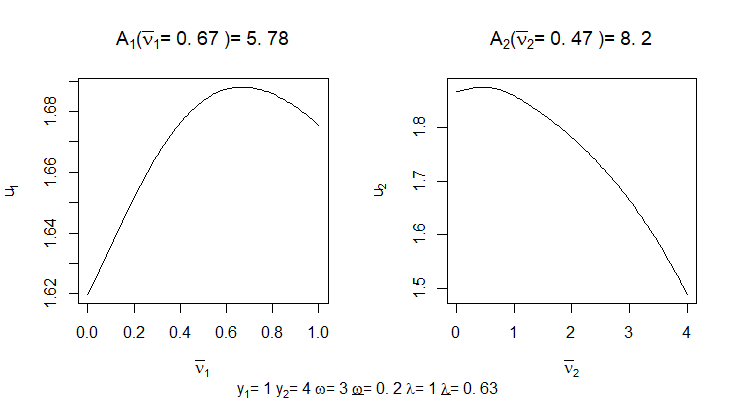
\includegraphics[width=5in]{subchapters/chapter3_images/LTAselection_plots}
\par\end{centering}
\caption{\label{fig:selection_with_omegabar_1}Selection of $\bar{\nu}_{1}$
and $\bar{\nu}_{2}$ for $u(A)=A^{1/3}$ }
\end{figure}

\begin{figure}
\begin{centering}
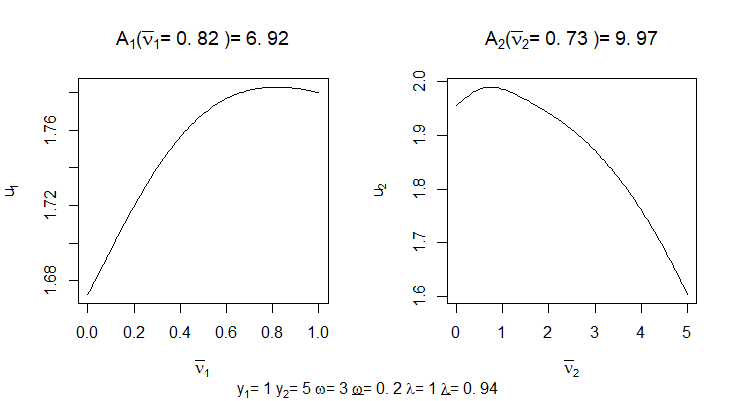
\includegraphics[width=5in]{subchapters/chapter3_images/LTAselection_plots_ychgconstomegabar}
\par\end{centering}
\caption{\label{fig:selection_with_omegabar_higher_y2}Selection of $\bar{\nu}_{1}$
and $\bar{\nu}_{2}$ for $u(A)=A^{1/3}$ with a higher income (same
$\text{\ensuremath{\underbar{\ensuremath{\omega}}}}$)}
\end{figure}

\begin{figure}
\begin{centering}
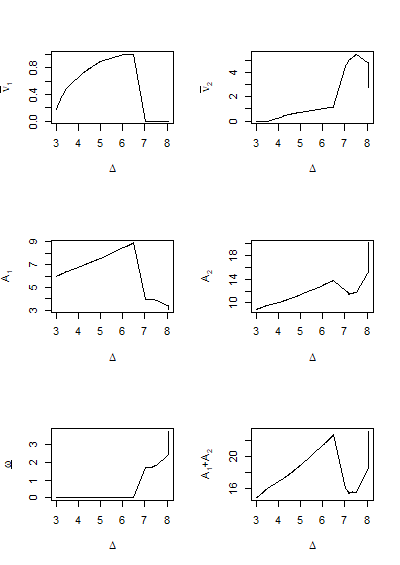
\includegraphics[width=3.2in]{subchapters/chapter3_images/omega_bar_sensitivity}
\par\end{centering}
\caption{\label{fig:nu1nu2_A1A2_exogenous_varsplot}Changes in$\bar{\nu}_{1}$,
$\bar{\nu}_{2}$ , $A_{1}$,$A_{2}$ implied with the utility ordering$\mathscr{U}(u_{1},u_{2})=\beta u_{1}+(1-\beta)u_{2}$}
\end{figure}

% g <- r[seq(586,1010),]; plot(g$nu2-g$nu1, g$omega_bar,type='l')
% par(mfrow=c(2,2));plot(g$y2-g$y1,g$nu1,type='l',xlim=c(0,8),ylim=c(0,5));plot(g$y2-g$y1,g$nu2,type='l',xlim=c(0,8),ylim=c(0,5)); plot(g$y2-g$y1,g$omega_bar,type='l',xlim=c(0,8),ylim=c(0,5))

The changes in $\bar{\nu}_{1}$ and $\bar{\nu}_{2}$ with respect
to changes in $\Delta=y_{2}-y_{1}$ are shown in Figure \ref{fig:nu1nu2_A1A2_exogenous_varsplot}.
As the figure shows, the very low values of $\underline{\omega}$
only make the status competition lucrative for the poorer consumer.
However, there is only a certain level of $\Delta\equiv y_{2}-y_{1}$until
which high income differences encourage only consumer 1 to increase
$\bar{\nu}_{1}$ - a level after which both consumers participate
so that $\bar{\nu}_{1}>0$ and $\bar{\nu}_{2}>0$. When $\underline{\omega}$
rises by as much that the poorer consumer is no longer able to afford
raising $\bar{\nu}_{1}$ , the optimal choice for consumer 1 is to
reduce $\bar{\nu}_{1}\rightarrow0$ - thus letting consumer 2 pay
for the high security implied by high $\bar{\omega}$. In other words,
an extremely large change in income differences reverses the withdrawal
among the consumers - since a shift from low-income differences to
high income-differences (through lowering of $y_{1}$ or increase
in $y_{2}$) causes the poorer consumer to no longer view any benefit
from the status investment - a situation where any further rise in
income differences only increases the investment $\bar{\nu}_{2}$
for consumer 2. Likewise, a shift from high-income differences to
largely-similar income-differences would mean that the richer consumer
no longer sees any benefit from participating in the status competition
- thus setting $\bar{\nu}_{2}$ to zero. Therefore, the lower differences
in income - which is used to accumulate assets in the long-term -
are as undesirable for the richer consumer as higher differences in
income are for the poorer consumer. A widening in income-differences
increases $\bar{\nu}_{1}$ and $\bar{\nu}_{2}$ - only until it becomes
so high $\bar{\nu}_{1}$ is reduced to zero by the consumer 1. Similarly,
a lowering of income differences decreases $\bar{\nu}_{1}$ and $\bar{\nu}_{2}$
until the incomes are so equal that $\bar{\nu}_{2}$ is reduced to
zero.

The equilibrium levels of asset accumulations also correspond to the
choices $\bar{\nu}_{1}$ and $\bar{\nu}_{2}$. An equilibrium with
high $\bar{\nu}_{1}$ and $\bar{\nu}_{2}$ does not necessarily mean
lower asset accumulations - since status investments also contribute
to asset accumulation through social promotion in the model. The total
asset accumulations implied by the selections $\bar{\nu}_{1}$ and
$\bar{\nu}_{2}$ in Figures \ref{fig:selection_with_omegabar_1} and
\ref{fig:selection_with_omegabar_higher_y2} demonstrate that $A_{1},A_{2}$
rise with rise in $\Delta=y_{2}-y_{1}$ if $\underline{\omega}$ remains
the same. With changes in $\underline{\omega}$, the total assets
decline for the poorer consumer on withdrawal (i.e. when $\bar{\nu}_{1}\rightarrow0$)
and they rise for consumer 2 with rise in income difference. As the
plots in Figure \ref{fig:nu1nu2_A1A2_exogenous_varsplot} show, a
high $A_{1}+A_{2}$ is achieved when all of the poorer consumer's
disposable income $y_{1}$ is spent towards status investments. The
withdrawal from status investments lowers the total accumulation $A_{1}+A_{2}$
until the point when changes in income difference $\Delta$ become
so high that all gains through status investments only benefit the
richer consumer. The result that total assets are higher either when
status investments are at highest possible values for the poor consumer
or when they benefit only the richer consumer in the long-term does
confirm the intuition as well.

% What's the QUESTION? -  The relationship between the sharp separation caused by \omega and the degree to which consumers enjoy their own reference group are not interesting enough.
% 1. In the population that could be greedy or content overall, is the consumer worse off for a given omega vs lambda (Do difference in y2-y1 have an effect on nu and A. Are consumers better off with reducing differences in y2-y1 or improving status competitions instead?)
% 2. Within a regime, does rise omega/lambda change A ?
% 3. Does y2-y1 create higher nu than steepness of omega?
% 4. Does more satisfaction with lower income band increase require a higher omega_bar for the equilibirum?

% see solution for the following for peak :
% two_stage_sol(omega_bar = 1,omega = 1,lambda_bar = 1,lambda = 1,G1 = 1.27,G2 = 1, y1= 1,y2 = 10  ,alpha = .3)
% two_stage_sol(omega_bar = 1,omega = 1,lambda_bar = 1,lambda = .2,G1 = 1.27,G2 = 1, y1= 1,y2 = 10  ,alpha = .3)

% two_stage_sol(omega_bar = .5,omega = 2,lambda_bar = 6,lambda = 1,G1 = 2,G2 = 1,y1 = .9,y2 = 10,alpha =.3 )

%For TNZ/NGR, above could give us the values of y_1 y_2 (we don't observe y_1,y_2 - except the small income data which we can associate with occupation).
%We can compare G1/G2 in the NGR/TNZ - but a better analysis of G1/G2 with lambda_bar,omega_bar and omega,lambda is needed.
%For SA/others, income data or occupation levels may be used.

% lambda = .1 ; bar_lambda = 50; x<-seq(0,100,.1); plot(x,1/(1+exp(-lambda * (x-bar_lambda))),type='l',xlab=latex2exp::TeX("$\\nu$"),ylab=latex2exp::TeX("$W(\\nu)$"),lty=1); 

%%%
%% Empirical Test 
%%%
% Notice that asset-costs as a function of assets is only an imagination. The costs imposed by assets are not fully captured in the reported asset-costs in the empirical data. A function that combines the  costs imposed by cars with costs imposed by houses - needs to average over a lot of thing. For the for fitting purposes itself, estimating a function that considers the number cars and houses owned would have be better - but that isn't what we're concerned with. For this reasons, the asset-cost function shape must not be relied on. Instead how a given fitted value of cost-function would impact the net equilibrium is more interesting. We are interested only in the condition in Equation  being satisfied - without estimating the entire function itself. Therefore, the assumption with a known cost-function (whatever its shape as long as the two consumers are on either side of the inflection point) must suffice.
% We use the above framework to test how we can compare how local per-head non-durable consumption could "indicate" status in an economy and if i) asset and income differences are stable, ii) populations are relatively stable of occupation ranks. If consumers can be believed to act as if a certain reward function existed, then do their non-durable consumption trends imply (we take South Africa or Tanzania) a different probability trends. The difference between SA and Tanzania are social. Assuming that asset differences and occupational differences are stable. What are the fundamental differences in the status competitions implied by the non-durable consumption levels.

%quantile(unique(ng$df2010$mean_A0),seq(10)/10)

% So given two bands (made of occupation-rank or otherwise), we need a solution conditions that does not depend on a particular form of cost-function. % But we know that there are many classes operating within an economy. We take interest in the just occupation_rank based populations - looking at the differences between occupation_rank = 1 and occupation_rank \in{2,3}. We can see how asset-costs behave in between these two and assume a smooth structure between the two - instead of attempting estimation of asset based function which is far too noisy. A_{0} for us is therefore a combination of occupation rank, usual assets and regional differences as well (anything that the consumer gains in the competition). The cost-function can therefore be hardly estimated.

% DATA can be analysed for South Africa
%ddply(ddd,.(max_occupation_rank),summarise,n=length(hhid2010))

\noindent

\newpage

\section{\label{sec:Conclusions-1}Conclusions}

% HK: a more affluent society will have lower utility at each income level. Hence, an increase in average income may be consistent with a decrease in social welfare. More plausibly, social welfare may rise only slowly in response to economic growth. 
% HK: poor are made worse off by greater equality. Such an increase in equality will also increase conspicuous  waste by those on middle incomes or low and middle incomes, while conspicuous consumption by the rich may decrease (our finding too). consequently, when we consider corrective taxes on conspicuous consumption, we find that the more equally income is distributed, the higher taxes and subsidies should be for those with low to middle incomes, and the lower they should be  or those with high incomes. Indeed, we are able to show that in some circumstances a corrective policy with higher tax rates (but also higher subsidies) for those with low incomes can lead to a Pareto improvement
% HK: Reducing inequality increases competition.

\noindent

We had set ourselves to find how income inequality could influence
status consumption as investments in an economy. Interpreting status
consumption as investments or efforts spent towards economic status,
we use a two-band economy under the conditions of population stability
and a known ordering of asset utilities for consumers to argue that
a rise in income inequalities need not always raise status consumption
in the long-term.

The conditions that population stability must prevail in a long-term
equilibrium of income bands and that there exists a known ordering
for asset utilities for the rich and poor consumer - together imply
that the expenditure towards status for the poorer (richer) consumer
need not rise (fall) with increase in income differences since withdrawal
of either the rich or the poor consumer. This is because an increase
(decrease) in income inequalities can drive an increase (decrease)
in status investments only as long as the poorer (richer) consumer
does not withdraw from the status game - finding it no longer lucrative
for positional improvement in the game. Thus, while it is tempting
to argue using the short-term equilibrium conditions that wider income
differences make status competitions more stringent and the expenditure
towards status higher (lower) for the poorer (richer) consumer, the
long-term equilibrium - under conditions of population stability and
a known order of asset utilities for the rich and the poor consumer
- imply a different dynamics where wide income differences could reduce
expenditure towards status by making promotion difficult (for the
poor consumers) or security cheaper (for the richer consumers). This
also means that the combined asset accumulations for the rich and
the poor consumer - might either rise or fall with higher income inequality.

%[Risk - TODO: Explain RISK]

There are two important caveats to the above result that we must also
highlight. First is that the cooperative solution rests on a certain
ordering of combined utility for rich and poor consumers. Second is
that a risk with the accumulated wealth is necessary for there to
be a status competition at all - one that promises income opportunities
and securities to the respective positions in a finite-bands setting.
In other words, an inequality in bands cannot maintain a steady state
competition without an inherent risk that sets an upper bound on wealth
accumulation for the richer consumer. 

%[Positive externality consumption falls]

In applications where consumer welfare follows from status investments
such as education, the above model can be used to explain how constraints
on resources in an economy with income segregation may limit the participation
of poorer consumers despite an increase in opportunities for income
mobility. The consideration of positional concerns of the economy
in the model demonstrates how long-term constraints due to finite
resources could lower the participation for investments such as education
simply because the differences in socioeconomic positions must also
be maintained. 

% We believe that the framework of risk used in the chapter could be extended further with the reference-aware risk-aversion or the non-linear response risk reference to further our understanding of the effect of relative income on status consumption.
% By pinning down a probability function for transitions through income bands, the model can also be used to view the redistribution in an economy as the security costs (or losses) implied by the promotion and demotion functions that the richer consumers must pay to maintain the higher income position. The contest-theory approach presented in the chapter thus also presents an opportunity to understand long-term implications of status competitions without choosing a specific redistribution mechanism such as taxation.

% 1. Increasing omega_bar for \lambda=1,\omega=3 from .3 to .9 would force the consumer 1 to become risky and require a higher lambda_bar (from 1.04 to 1.5). This trend remains the same even for a higher \kappa. This means that a higher security threshold is also needed as consumer promotion gets crowded when omega_bar rises (this does not change with rising \kappa). This explains status consumption is symmetrical.
% 2. Changes in required y1,y2   
% (a) required y2: 
% i. With fixed \lambda=1,\omega=2 \underline{\omega}=.3, we find that the income y2 of equilibrium rises with rise in \underline{\lambda} (raising \underline{\lambda} from from 1.2 to 1.9 raises y2 from 5.13 to 7.8). With fixed y1, increasing status consumption security would increases y_{2}.  
% ii. With fix \lambda=1,\omega=2 \underline{\lambda}=1.2, y_{1}=1, increasing \underline{\omega} from .3 to .5 decreases y2 - the poorer consumer is poised to spend all her income in status consumption - so making competition more difficult for the poorer consumer a lesser income difference y_{2}-y_{1}. Decreasing \underline{\omega} similarly increases y_{2} because making competition easier for the poorer consumer would require a higher y_{2}. Easier competition also makes more y_{2} necessary. 
% (b) required y1, we fix y_{2}=5,\kappa=4,   
% i. \underline{\omega}=.2 - decreasing \underline{\lambda} from .85 to .82 decreases y1 and increasing \underline{\lambda} increases y_{1}. More costs for security require higher income for poor consumer.   
% ii. \underline{\lambda}=1.2 , inceasing \underline{\omega} increases y_{1}.   
% 3. Effect of y_{2}-y_{1} under non-segregated consumption - no  

% (a) \underline{\lambda} - Narrowing y_{2}-y_{1}- decreases \underline{\lambda} - thus the security level required falls for the same \underline{\omega}. The security becomes cheaper for less narrower income. When income difference is high the richer consumer are happy to spend on status consumption. Giving more income to the poor reduces the security required!! This is surprising. This seems to happen because giving more assets to the poor makes the rich-position less worthwhile - This is assuming that assets is all what people want. This happens in a mobile environment when \omega\ne\lambda.   
% i. With \kappa=3,\underline{\omega}=.3,y_{2}=7 , Increasing y_{1} (from 2 to 3) from reduces \underline{\lambda} (from 1.2 to 1.0) and decreasing y_{1} (from 1.5 to 2) increases it (from 1.03 to 1.36)
% get_no_greed_missing_var(fixed_varname = "lambda_bar_y1",fixed_varval =3, plot = T). With \kappa<1, increasing y_{1} also decreases \underline{\lambda}. This may be because we are not optimising sharply - but it is still a good approximation.  
% ii. With \kappa=3,\underline{\omega}=.2,y_{1}=1 , increasing y_{2}(from 3 to 4) increases \underline{\lambda}( from .09 to .6) and decreasing y_{2}(from 3 to 2) decreases it (from .09 to .00005 ) %get_no_greed_missing_var(fixed_varname = "lambda_bar_y2",fixed_varval = 5, plot = T)   
% (b) \underline{\omega} - Narrowing y_{2}-y_{1}- increases \underline{\omega}.  Basically, narrowing income seems to make \underline{\omega} higher
% i. With \kappa=10, \lambda=1,\underline{\lambda}=3,y_{2}=12, increasing y_{1} (from 5 to 5.2) increases \underline{\omega} from 2.48 from 2.5 %get_no_greed_missing_var(fixed_varname = "omega_bar_y1",fixed_varval = 5 , plot = T)   
% ii. With \kappa=2, \lambda=1,\underline{\lambda}=.2,y_{1}=2, increasing y_{2} (from 4.75 to 5) decreases \underline{\omega} from .3 to 1e-5 %get_no_greed_missing_var(fixed_varname = "omega_bar_y2",fixed_varval = 4.75 , plot = T)

% [Next: greed and loss-aversion] When consumers have a preference for lower assets in the low band, the introduction of greed or contentment would can shift the equilibrium further. Contentment is just the name of loss-aversion associated. Consumers might be less loss-averse with respect to A_{0} in which case they are more content with lower than A_{0}. On the other hand, they might be in a regime where consumers don't like being less than A_{0} at all. We look at the contentment vs aspiration in the above setup for a given \kappa . The consumer utility uses a reference function defined around long-term A_{0} so that there are two regimes. First, where being poor may not become successively bad. Second, is the regime where contentment is valuable and the consumer below A_{0} don't mind it too much compared to how much consumers with more wealth... . The other regime is when consumer are more greedy and people mind being poor a lot compared to being rich. We see how either of these regimes are influenced by \kappa vs y_{2}-y_{1}(This way we don't need to deal with measurement of g1/g2 but we can argue only what greed and contentment with assets implies). Greed can help us relieve the stringent \overline{\nu}_{2}<\frac{\underbar{\ensuremath{\omega}}}{\kappa}+\overline{\lambda} and \nu_{1}^{*}<\underbar{\ensuremath{\kappa}\ensuremath{\ensuremath{\lambda}}+}\underbar{\ensuremath{\omega}}. Future applications could apply risk-aversion levels.This needs to be explored further. 
% With Greed Observations
% 1. Giving more income to the poor might
% 2. Greed: A consumer can be greedy or contented. She would accept an increase in y1 when she is poor. When she is subjectively greedy she would expect more. But does that really make her better off?

\newpage

\section*{\centering{APPENDIX I}} 

We know that for $y'(t)=a(t)y(t)+b(t)$ and $y(t_{0})=y_{0}$ we have
the solution

\begin{alignat}{1}
y(t) & =y_{0}e^{A(t)}+e^{A(t)}\int_{t_{0}}^{t}e^{-A(s)}b(s)ds\label{eq:general_solution}
\end{alignat}
 

Here, $A(t)=\int_{t_{0}}^{t}a(s)ds$.

Given $u(A)=\Gamma A^{\alpha}$, we have

\begin{gather*}
W(\nu)u_{2}(A+y_{1}-\nu+y_{2})+(1-W(\nu))u_{1}(A+y_{1}-\nu+y_{1})\\
=W(\nu)\Gamma(A+y_{1}-\nu+y_{2})^{\alpha}+(1-W(\nu))\Gamma(A+y_{1}-\nu+y_{1})^{\alpha}
\end{gather*}

We rewrite the function $f(\nu)$ which is to be maximised by choosing
$M_{1}=A+y_{1}+y_{1}$and $M_{2}=A+y_{1}+y_{2}$.

\begin{gather*}
f(\nu)=W(\nu)(\Gamma(A+y_{1}-\nu+y_{2})^{\alpha}-\Gamma(A+y_{1}-\nu+y_{1})^{\alpha})+\Gamma(A+y_{1}-\nu+y_{1})^{\alpha}\\
\Rightarrow f(\nu)=W(\nu)(\Gamma(M_{2}-\nu)^{\alpha}-\Gamma(M_{1}-\nu)^{\alpha})+\Gamma(M_{1}-\nu)^{\alpha}
\end{gather*}
 

The derivative $f'(\nu)$ 

\begin{multline*}
f'(\nu)=(\Gamma(M_{2}-\nu)^{\alpha}-\Gamma(M_{1}-\nu)^{\alpha})W'(\nu)\\
+W(\nu)(\alpha\Gamma(M_{1}-\nu)^{\alpha-1}-\alpha\Gamma(M_{2}-\nu)^{\alpha-1})-\alpha\Gamma(M_{1}-\nu)^{\alpha-1}
\end{multline*}

The first order condition $f'(\nu)$ implies

\begin{multline*}
f'(\nu)=0\Rightarrow(\Gamma(M_{2}-\nu)^{\alpha}-\Gamma(M_{1}-\nu)^{\alpha})W'(\nu)\\
=W(\nu)(\alpha\Gamma(M_{2}-\nu)^{\alpha-1}-\alpha\Gamma(M_{1}-\nu)^{\alpha-1})+\alpha\Gamma(M_{1}-\nu)^{\alpha-1}
\end{multline*}

\begin{alignat*}{1}
W'(\nu) & =\alpha W(\nu)\frac{(M_{2}-\nu)^{\alpha-1}-(M_{1}-\nu)^{\alpha-1}}{(M_{2}-\nu)^{\alpha}-(M_{1}-\nu)^{\alpha}}+\frac{\alpha(M_{1}-\nu)^{\alpha-1}}{(M_{2}-\nu)^{\alpha}-(M_{1}-\nu)^{\alpha}}
\end{alignat*}

The characteristic function $A(t)=\int a(s)ds$ in the Equation \ref{eq:general_solution}
corresponds to the following (notice that this is defined only as
long as $(M_{1}-\nu)^{\alpha}\ne(M_{2}-\nu)^{\alpha}$)

\begin{alignat*}{1}
\int a(s)ds & =-log(\Gamma(M_{1}-\nu)^{\alpha}-\Gamma(M_{2}-\nu)^{\alpha})+C
\end{alignat*}

Writing $D=log(\Gamma_{1}(M_{1})^{\alpha}-\Gamma_{2}(M_{2})^{\alpha})$
we have

\begin{gather*}
A(\nu)=\int_{0}^{\nu}a(s)ds=-log(\Gamma(M_{1}-\nu)^{\alpha}-\Gamma(M_{2}-\nu)^{\alpha})-(-log(\Gamma(M_{1})^{\alpha}-\Gamma(M_{2})^{\alpha}))\\
=log(\Gamma(M_{1})^{\alpha}-\Gamma(M_{2})^{\alpha})-log(\Gamma(M_{1}-\nu)^{\alpha}-\Gamma(M_{2}-\nu)^{\alpha})\\
=D-log(\Gamma(M_{1}-\nu)^{\alpha}-\Gamma(M_{2}-\nu)^{\alpha})
\end{gather*}

Thus,

\begin{alignat*}{1}
A(\nu) & =D-log(\Gamma(M_{1}-\nu)^{\alpha}-\Gamma(M_{2}-\nu)^{\alpha})
\end{alignat*}

and,

\begin{alignat*}{1}
e^{-A(s)} & =e^{log(\Gamma(M_{1}-s)^{\alpha}-\Gamma(M_{2}-s)^{\alpha})-D}=e^{-D}(\Gamma(M_{1}-s)^{\alpha}-\Gamma(M_{2}-s)^{\alpha})
\end{alignat*}

Therefore,

\begin{alignat*}{1}
e^{A(\nu)} & =\frac{e^{D}}{\Gamma(M_{1}-\nu)^{\alpha}-\Gamma(M_{2}-\nu)^{\alpha}}
\end{alignat*}

Now 
\begin{gather*}
\int_{\nu_{0}}^{\nu}e^{-A(s)}b(s)ds=\int_{\nu_{0}}^{\nu}e^{-D}(\Gamma(M_{1}-s)^{\alpha}-\Gamma(M_{2}-s)^{\alpha})\times\frac{\alpha(M_{1}-s)^{\alpha-1}}{(M_{2}-s)^{\alpha}-(M_{1}-s)^{\alpha}}\\
=-\alpha e^{-D}\Gamma\int_{\nu_{0}}^{\nu}(M_{1}-s)^{\alpha-1}
\end{gather*}

The integration of the last term is 

\begin{alignat*}{1}
\int_{\nu_{0}}^{\nu}(M_{1}-s)^{\alpha-1} & =-\frac{1}{\alpha}(M_{1}-s)^{\alpha}|_{\nu_{0}}^{\nu}=-\frac{1}{\alpha}((M_{1}-\nu)^{\alpha}-(M_{1}-\nu_{0})^{\alpha})
\end{alignat*}

Therefore,

\begin{alignat*}{1}
\int_{\nu_{0}}^{\nu}e^{-A(s)}b(s)ds & =-\alpha e^{-D}\Gamma(-\frac{1}{\alpha}((M_{1}-\nu)^{\alpha}-(M_{1}-\nu_{0})^{\alpha}))=\frac{\Gamma((M_{1}-\nu)^{\alpha}-(M_{1}-\nu_{0})^{\alpha})}{e^{D}}
\end{alignat*}

and

\begin{multline}
W(\nu)=W(\nu_{0})e^{A(\nu)}+e^{A(\nu)}\int_{\nu_{0}}^{\nu}e^{-A(s)}b(s)ds\\
=\frac{W(\nu_{0})(M_{2}{}^{\alpha}-M_{1}{}^{\alpha})}{(M_{2}-\nu)^{\alpha}-(M_{1}-\nu)^{\alpha}}+\frac{(M_{1}-\nu_{0})^{\alpha}-(M_{1}-\nu)^{\alpha}}{(M_{2}-\nu)^{\alpha}-(M_{1}-\nu)^{\alpha}}\label{eq:solution_1-1}
\end{multline}

Equivalently for the $L(\nu)$, we have 

\begin{alignat*}{1}
L'(\nu) & =L(\nu)\alpha\frac{(M_{1}-\nu)^{\alpha-1}-(M_{2}-\nu)^{\alpha-1}}{(M_{1}-\nu)^{\alpha}-(M_{2}-\nu)^{\alpha}}+\frac{\alpha(M_{2}-\nu)^{\alpha-1}}{(M_{1}-\nu)^{\alpha}-(M_{2}-\nu)^{\alpha}}
\end{alignat*}

Again, the characteristic function is as follows

\begin{alignat*}{1}
A(\nu) & =D-log(\Gamma(M_{1}-\nu)^{\alpha}-\Gamma(M_{2}-\nu)^{\alpha})
\end{alignat*}

Therefore,

\begin{alignat*}{1}
e^{A(\nu)} & =\frac{e^{D}}{\Gamma(M_{1}-\nu)^{\alpha}-\Gamma(M_{2}-\nu)^{\alpha}}
\end{alignat*}

Further,

\begin{gather*}
\int_{\nu_{0}}^{\nu}e^{-A(s)}b(s)ds=\int_{\nu_{0}}^{\nu}e^{-D}(\Gamma(M_{1}-s)^{\alpha}-\Gamma(M_{2}-s)^{\alpha})\times\frac{\alpha(M_{2}-s)^{\alpha-1}}{(M_{1}-s)^{\alpha}-(M_{2}-s)^{\alpha}}\\
=-\alpha e^{-D}\Gamma\int_{\nu_{0}}^{\nu}(M_{2}-s)^{\alpha-1}
\end{gather*}

The integration of the last term is 

\begin{alignat*}{1}
\int_{\nu_{0}}^{\nu}(M_{2}-s)^{\alpha-1} & =-\frac{1}{\alpha}(M_{2}-s)^{\alpha}|_{\nu_{0}}^{\nu}=-\frac{1}{\alpha}((M_{2}-\nu)^{\alpha}-(M_{2}-\nu_{0})^{\alpha})
\end{alignat*}

Therefore,

\begin{alignat*}{1}
\int_{\nu_{0}}^{\nu}e^{-A(s)}b(s)ds & =\frac{\Gamma((M_{2}-\nu)^{\alpha}-(M_{2}-\nu_{0})^{\alpha})}{e^{D}}
\end{alignat*}

The solution for $L(\nu)$ is therefore

\begin{alignat*}{1}
L(\nu) & =\frac{L(\nu_{0})((M_{1})^{\alpha}-(M_{2})^{\alpha})}{(M_{1}-\nu)^{\alpha}-(M_{2}-\nu)^{\alpha}}+\frac{(M_{2}-\nu)^{\alpha}-(M_{2}-\nu_{0})^{\alpha}}{(M_{1}-\nu)^{\alpha}-(M_{2}-\nu)^{\alpha}}
\end{alignat*}

\pagebreak
\section*{\centering{APPENDIX II}} 

The proof to demonstrate the lack of feasible non-constant $W(\nu)$,
$L(\nu)$ that lead to stable asset-values in an economy with different
income bands uses a general cost-function associated with the level
of assets $A$. This function $c(A)$ is used to explain how consumers
in the long-term equilibrium may balance future expected income with
the costs imposed by the current assets. In empirical terms, this
may correspond to expected expenditure required to maintain a certain
level of wealth - including any maintenance fees, interest on loan,
club memberships etc. that are associated with a certain level of
wealth. We also define a net asset value function based on the general
cost-function $c(A)$ that represents the net value of assets after
adjusting for asset-costs

\begin{align}
\pi(A) & =A-c(A)\label{eq:net_asset_value_def}
\end{align}

Note that even if the consumer were allowed to use leverage (credit)
by choosing costs higher than she can afford, the liquidity concerns
would ensure that $\nu_{1}<y_{1}$ and $y_{2}<\nu_{2}$. We now state
the proof that no $W(\nu),L(\nu)$ would result in stable asset allows
under no-risk and under population stability conditions.
\begin{thm*}
\label{thm:NoLTEWithoutRisk}There exist no $\pi(A)$ and non-constant
$W_{1}(\nu)$,$L_{2}(\nu)$ for the long-term equilibrium satisfying
the population constraint for asset accumulations under no risk.
\end{thm*}
\begin{proof}
The proof is stated for two bands and can be generalised for higher
number of bands. Notice that the population-stability constraint for
the two band-economy means the following condition for $W(\prescript{t}{}\nu_{1})$
and $L(\prescript{t}{}\nu_{2})$ where $\prescript{t}{}\nu_{1}$,
$\prescript{t}{}\nu_{2}$ are the expenditure towards status values
selected by the consumer in band 1 and 2 at period $t$ respectively

\begin{align}
W(\prescript{t}{}\nu_{1}) & =L(\prescript{t}{}\nu_{2})\label{eq:two_band_population_stability}
\end{align}

Next, the long-term equilibrium implies a stability of asset levels
so that no more long-term asset-value is added to the consumer's assets
as she chooses the equilibrium $\prescript{t}{}\nu_{1}$ (consumer
1) or $\prescript{t}{}\nu_{2}$ (consumer 2). Thus, with $\prescript{t}{}A_{1},\prescript{t}{}A_{2}$
as the asset values at time $t$ and the net asset value function
$\pi(A)$ in equilibrium (see Equation \ref{eq:net_asset_value_def}),
the assets would stabilise at $\prescript{t}{}A_{1}$ for consumer
1 and $\prescript{t}{}A_{2}$ for consumer 2 in the long-term equilibrium
only as long as the following quantity tends to zero for the consumer
1 (as non-zero increments prevent stability of asset-values)

\begin{alignat*}{1}
W(\prescript{t}{}\nu_{1})\pi(\prescript{t}{}A_{1}-\prescript{t}{}\nu_{1}+y_{2})+(1-W(\prescript{t}{}\nu_{1}))\pi(\prescript{t}{}A_{1}-\prescript{t}{}\nu_{1}+y_{1}) & \rightarrow0
\end{alignat*}

\begin{align}
W_{1}(\prescript{t}{}\nu_{1}) & =\frac{1}{1-\frac{\pi(\prescript{t}{}A_{1}-\prescript{t}{}\nu_{1}+y_{2})}{\pi(\prescript{t}{}A_{1}-\prescript{t}{}\nu_{1}+y_{1})}}\label{eq:w_lte}
\end{align}

The above condition implies that the consumer balances her expected
future income with the costs on her assets. The net asset value from
being either in band 1 or band 2 would be balanced by the expected
returns the consumer 1 gets from putting up $\nu_{1}$ towards status
competitions. Since the probability $W_{1}(\nu)$ must be positive
and less than unity, the ratio $\frac{\pi(\prescript{t}{}A_{1}-\prescript{t}{}\nu_{1}+y_{2})}{\pi(\prescript{t}{}A_{1}-\prescript{t}{}\nu_{1}+y_{1})}$
must be less than zero. In other words, the consumer in band 1 must
move from a negative net asset-value to a positive asset value in
band 2 (or vice versa). Similarly, for the consumer in band 2, the
following quantity must amount to zero in the long-term equilibrium

\begin{align*}
L_{2}(\prescript{t}{}\nu_{2})\pi(\prescript{t}{}A_{2}-\prescript{t}{}\nu_{2}+y_{1})+(1-L_{2}(\prescript{t}{}\nu_{2}))\pi(\prescript{t}{}A_{2}-\prescript{t}{}\nu_{2}+y_{2}) & \rightarrow0
\end{align*}

\begin{align}
L(\prescript{t}{}\nu_{2}) & =\frac{1}{1-\frac{\pi(\prescript{t}{}A_{2}-\prescript{t}{}\nu_{2}+y_{1})}{\pi(\prescript{t}{}A_{2}-\prescript{t}{}\nu_{2}+y_{2})}}\label{eq:l_lte}
\end{align}

Above ensures that the expected loss from being in band 1 is balanced
by the security provided by $1-L_{2}(\nu_{2})$. For consumer 2, $\frac{\pi(\prescript{t}{}A_{2}-\prescript{t}{}\nu_{2}+y_{1})}{\pi(\prescript{t}{}A_{2}-\prescript{t}{}\nu_{2}+y_{2})}$
must also be less than zero when she moves from a negative net asset
value in band 2 to a positive net asset-value in 1 (or vice versa).

As $\prescript{t}{}A_{1}$ and $\prescript{t}{}A_{2}$ stabilise in
the long-term we drop the subscript $t$ to write $\prescript{t}{}A_{1}\rightarrow A_{1}^{*}$
and $\prescript{t}{}A_{2}\rightarrow A_{2}^{*}$ . Similarly, we write
$\prescript{t}{}\nu_{1}\rightarrow\nu_{1}^{*}$and $\prescript{t}{}\nu_{2}\rightarrow\nu_{2}^{*}$
. Combining the population stability condition in Equation \ref{eq:two_band_population_stability}
with the long-term asset stability conditions in Equations \ref{eq:w_lte}
and \ref{eq:l_lte} we can write

\begin{align}
\frac{\pi(A_{1}^{*}-\nu_{1}^{*}+y_{2})}{\pi(A_{1}^{*}-\nu_{1}^{*}+y_{1})} & =\frac{\pi(A_{2}^{*}-\nu_{2}^{*}+y_{1})}{\pi(A_{2}^{*}-\nu_{2}^{*}+y_{2})}<0\label{eq:cost_function_shape}
\end{align}

As long as status competition is feasible for consumer 1, she should
see an increase in the long-term net asset value by being in band
2. The possibility of moving from band 1 to band 2 only to observe
the net asset value decline is ruled out because higher income bands
are also meant to have a higher asset reference. Any peer effects
associated with the assets would ensure a higher asset (comparative)
reference in the higher asset-band. Thus while the consumer in band
1 cannot afford to have a decline in net asset value if she moves
to the next band, the consumer in the rich band might accept a poorer
band with a net increase in asset value. This implies that the the
net asset-value function must be concave (see Figure \ref{fig:asset_value_function_demo}). 

However, the long-term equilibrium also ensures that the consumer
arriving from the different band gathers no more assets than other
consumers in the same band. Thus, we also have

\begin{gather}
\pi(A_{1}^{*}-\nu_{1}^{*}+y_{2})=\pi(A_{2}^{*}-\nu_{2}^{*}+y_{2})\nonumber \\
\pi(A_{2}^{*}-\nu_{2}^{*}+y_{1})=\pi(A_{1}^{*}-\nu_{1}^{*}+y_{1})\label{eq:stability_2}
\end{gather}

%A concave net asset value function eventually corresponds to convex costs associated with the asset - which is plausible when there costs increase both for extremely high wealth levels and for extremely low wealth levels.

Due to Equation \ref{eq:cost_function_shape} and \ref{eq:stability_2},
an equilibrium is implied only if 

\begin{align*}
\pi(A_{1}^{*}+y_{1}-\nu_{1}^{*}) & +\pi(A_{2}^{*}+y_{2}-\nu_{2}^{*})=0
\end{align*}

\begin{figure}[H]
\begin{centering}
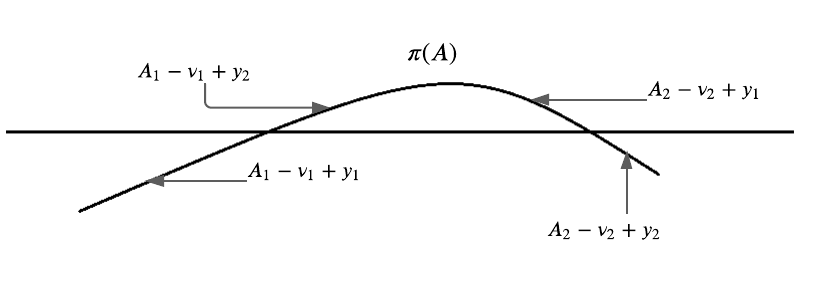
\includegraphics[width=4in]{subchapters/net_asset_function_demo}
\par\end{centering}
\caption{\label{fig:asset_value_function_demo} Asset value function necessitated
by the long-term equilibrium}
\end{figure}
Thus, the consumer must see no net gain on average from participating
in the status competition for$\prescript{t}{}A_{1}$ and $\prescript{t}{}A_{2}$
to have stable $A_{1}^{*},A_{2}^{*}$. The population constraint therefore
implies that $W(\nu_{1}^{*})=L(\nu_{2}^{*})=\frac{1}{2}$ as the only
possible equilibrium when no new asset value is added by participation
in status competitions.
\end{proof}
\newpage
\section*{\centering{APPENDIX III}} 

To express the consumer utilities $u_{1},u_{2}$ in terms of $\bar{\nu}_{1}$(or
equivalently in terms of $\bar{\nu}_{2}$) with the specific forms
of $W(\nu),L(\nu)$ defined in Section \ref{subsec:Equilibria-particular}
and $u(A)=\Gamma A^{\alpha}$, we consider first that

\begin{align*}
E_{1}(\bar{\nu}_{1}) & =W(\bar{\nu}_{1})y_{2}+(1-W(\bar{\nu}_{1}))y_{1}=L(\bar{\nu}_{2})y_{2}+(1-L(\bar{\nu}_{2}))y_{1}
\end{align*}

\begin{align*}
E_{2}(\bar{\nu}_{2}) & =W(\bar{\nu}_{1})y_{1}+(1-W(\bar{\nu}_{1}))y_{2}=(1-L(\bar{\nu}_{2}))y_{2}+L(\bar{\nu}_{2})y_{1}
\end{align*}

$u_{1}$ can now be written in terms of $\bar{\nu}_{1}$ using $\bar{\nu}_{2}=\phi(\bar{\nu}_{1})$
as follows

\begin{gather*}
u_{1}=W(\bar{\nu}_{1})u(y_{1}-\bar{\nu}_{1}+y_{2}-\bar{\nu}_{2}+E_{2}(\bar{\nu}_{2}))+(1-W(\bar{\nu}_{1}))u(y_{1}-\bar{\nu}_{1}+y_{1}-\bar{\nu}_{1}+E_{1}(\bar{\nu}_{1}))\\
\Rightarrow u_{1}=W(\bar{\nu}_{1})u(y_{1}-\bar{\nu}_{1}+y_{2}-\phi(\bar{\nu}_{1})+W(\bar{\nu}_{1})y_{1}+(1-W(\bar{\nu}_{1}))y_{2})\\
+(1-W(\bar{\nu}_{1}))u(2(y_{1}-\bar{\nu}_{1})+W(\bar{\nu}_{1})y_{2}+(1-W(\bar{\nu}_{1}))y_{1})
\end{gather*}

With the utility function $u(A)=\Gamma A^{\alpha}$ and the specific
forms for $W(\nu)$ and $L(\nu)$, $u_{1}$ and $u_{2}$ are thus

\begin{gather*}
u_{1}=\Gamma(3y_{1}-2\bar{\nu}_{1}+\frac{\Delta}{1+e^{-\omega(\bar{\nu}_{1}-\text{\ensuremath{\underbar{\ensuremath{\omega}}}})}})^{\alpha}\\
+\frac{\Gamma(3y_{1}-\bar{\nu}_{1}+2\Delta-\underbar{\ensuremath{\lambda}}+(\omega/\lambda)\bar{\nu}_{1}-(\omega/\lambda)\underbar{\ensuremath{\omega}}-\frac{\Delta}{1+e^{-\omega(\bar{\nu}_{1}-\text{\ensuremath{\underbar{\ensuremath{\omega}}}})}})^{\alpha}}{1+e^{-\omega(\bar{\nu}_{1}-\text{\ensuremath{\underbar{\ensuremath{\omega}}}})}}\\
-\frac{\Gamma(3y_{1}-2\bar{\nu}_{1}+\frac{\Delta}{1+e^{-\omega(\bar{\nu}_{1}-\text{\ensuremath{\underbar{\ensuremath{\omega}}}})}})^{\alpha}}{1+e^{-\omega(\bar{\nu}_{1}-\text{\ensuremath{\underbar{\ensuremath{\omega}}}})}}
\end{gather*}

\begin{gather*}
u_{2}=\frac{\Gamma(3y_{1}+\Delta-\underbar{\ensuremath{\lambda}}+(\omega/\lambda)\bar{\nu}_{1}-(\omega/\lambda)\underbar{\ensuremath{\omega}}-\bar{\nu}_{1}+\frac{\Delta}{1+e^{-\omega(\bar{\nu}_{1}-\text{\ensuremath{\underbar{\ensuremath{\omega}}}})}})^{\alpha}}{1+e^{-\omega(\bar{\nu}_{1}-\text{\ensuremath{\underbar{\ensuremath{\omega}}}})}}\\
-\frac{\Gamma(3y_{1}+3\Delta-2\underbar{\ensuremath{\lambda}}+(2\omega/\lambda)\bar{\nu}_{1}-(2\omega/\lambda)\underbar{\ensuremath{\omega}}-\frac{\Delta}{1+e^{-\omega(\bar{\nu}_{1}-\text{\ensuremath{\underbar{\ensuremath{\omega}}}})}})^{\alpha}}{1+e^{-\omega(\bar{\nu}_{1}-\text{\ensuremath{\underbar{\ensuremath{\omega}}}})}}\\
+\Gamma(3y_{1}+3\Delta-2\underbar{\ensuremath{\lambda}}+(2\omega/\lambda)\bar{\nu}_{1}-(2\omega/\lambda)\underbar{\ensuremath{\omega}}-\frac{\Delta}{1+e^{-\omega(\bar{\nu}_{1}-\text{\ensuremath{\underbar{\ensuremath{\omega}}}})}})^{\alpha}
\end{gather*}

The derivatives to be used for the first-order conditions are (setting
$F\equiv1+e^{-\omega(\bar{\nu}_{1}-\text{\ensuremath{\underbar{\ensuremath{\omega}}}})}$
) 

\begin{multline*}
\frac{\partial u_{1}}{\partial\bar{\nu}_{1}}=\frac{1}{F}\{\alpha\Gamma\times(-\frac{\Delta\omega(F-1)}{F^{2}}+\frac{\omega}{\lambda}-1)(2\Delta-\underline{\lambda}-\frac{\omega\underline{\omega}}{\lambda}-\frac{\Delta}{F}+\frac{\omega\bar{\nu}_{1}}{\lambda}-\bar{\nu}_{1}+3y_{1})^{\alpha-1}\\
-\alpha\Gamma\times(\frac{\Delta\omega(F-1)}{F^{2}}-2)(\frac{\Delta}{F}-2\bar{\nu}_{1}+3y_{1})^{\alpha-1}\}\\
+\frac{\omega(F-1)}{F^{2}}\{\Gamma\times(2\Delta-\underline{\lambda}-\frac{\omega\underline{\omega}}{\lambda}-\frac{\Delta}{F}+\frac{\omega}{\lambda}\bar{\nu}_{1}-\bar{\nu}_{1}+3y_{1})^{\alpha}-\Gamma\times(\frac{\Delta}{F}-2\bar{\nu}_{1}+3y_{1})^{\alpha}\}\\
+\alpha\Gamma\times(\frac{\Delta\omega(F-1)}{F^{2}}-2)(\frac{\Delta}{F}-2\bar{\nu}_{1}+3y_{1})^{\alpha-1}
\end{multline*}

\begin{multline*}
\frac{\partial u_{2}}{\partial\bar{\nu}_{1}}=\frac{1}{F}\{\alpha\Gamma\times(\frac{\Delta\omega(F-1)}{F^{2}}+\frac{\omega}{\lambda}-1)(\Delta-\underline{\lambda}+\frac{\Delta}{F}+\frac{\omega(\bar{\nu}_{1}-\underline{\omega})}{\lambda}-\bar{\nu}_{1}+3y_{1})^{\alpha-1}\\
-\alpha\Gamma\times(\frac{2\omega}{\lambda}-\frac{\Delta\omega(F-1)}{F^{2}})(3\Delta-2\underline{\lambda}-\frac{\Delta}{F}+\frac{2\omega(\bar{\nu}_{1}-\underline{\omega})}{\lambda}+3y_{1})^{\alpha-1}\}\\
+\frac{\omega(F-1)}{F^{2}}\{\Gamma\times(\Delta-\underline{\lambda}+\frac{\Delta}{F}+\frac{\omega(\bar{\nu}_{1}-\underline{\omega})}{\lambda}-\bar{\nu}_{1}+3y_{1})^{\alpha}\\
-\Gamma\times(3\Delta-2\underline{\lambda}-\frac{\Delta}{F}+\frac{2\omega(\bar{\nu}_{1}-\underline{\omega})}{\lambda}+3y_{1})^{\alpha}\}\\
+\alpha\Gamma\times(\frac{2\omega}{\lambda}-\frac{\Delta\omega(F-1)}{F^{2}})(3\Delta-2\underline{\lambda}-\frac{\Delta}{F}+\frac{2\omega(\bar{\nu}_{1}-\underline{\omega})}{\lambda}+3y_{1})^{\alpha-1}
\end{multline*}

Above only have $\underline{\lambda}$ and $\underline{\omega}$ as
unknowns - one of which can be eliminated using the population condition
- leaving the other unknown determined using the combined utility
function.

\newpage

\bibliographystyle{abbrv}
\bibliography{C:/local_files/research/africa_attitudes}

\end{document}
